\chapterimage{Pictures/chap02/dof-dragons-848.png}

\chapter{几何与变换}\label{chap:几何与变换}
\setcounter{sidenote}{1}

几乎所有非平凡\sidenote{译者注:原文nontrivial。}的图形程序都建立在几何类的基础上。
这些类表示数学概念例如点、向量以及射线。
因为这些类贯穿了整个系统,所以良好的抽象和高效的实现至关重要。
本章介绍了pbrt几何基础的接口和实现。
注意这些并不是表示实际场景几何体的类(三角形、球体等);
那些类是第\refchap{形状}的主题。

本章几何类在pbrt发行版的文件
\href{https://github.com/mmp/pbrt-v3/tree/master/src/core/geometry.h}{\ttfamily core/geometry.h}
和\href{https://github.com/mmp/pbrt-v3/tree/master/src/core/geometry.cpp}{\ttfamily core/geometry.cpp}
中定义,变换矩阵(\refsec{变换})在文件
\href{https://github.com/mmp/pbrt-v3/tree/master/src/core/transform.h}{\ttfamily core/transform.h}和
\href{https://github.com/mmp/pbrt-v3/tree/master/src/core/transform.cpp}{\ttfamily core/transform.cpp}
中实现。

\section{坐标系统}\label{sec:坐标系统}

按计算机图形学中的经典做法,
pbrt用三个坐标值$x,y$和$z$表示\keyindex{点}{point}{}、
\keyindex{向量}{vector}{}和\keyindex{法向量}{normal vector}{vector向量}。
这些值须在\keyindex{坐标系统}{coordinate system}{}下才有意义,
即定义了空间的原点并给出三个线性独立的向量定义$x,y$和$z$坐标轴。
总之,这样的原点和三个向量称为\keyindex{坐标系}{frame}{}。
给定3D中的任意一点或方向,其$(x,y,z)$坐标值取决于它和坐标系的关系。
\reffig{2.1}以2D形式给出例子说明了这点。
\begin{figure}[htbp]
    \centering%LaTeX with PSTricks extensions
%%Creator: Inkscape 1.0.1 (3bc2e813f5, 2020-09-07)
%%Please note this file requires PSTricks extensions
\psset{xunit=.5pt,yunit=.5pt,runit=.5pt}
\begin{pspicture}(327.3999939,474.47000122)
{
\newrgbcolor{curcolor}{0 0 0}
\pscustom[linewidth=1,linecolor=curcolor]
{
\newpath
\moveto(5.5,318.58000122)
\lineto(5.5,38.68000122)
\lineto(286.4,38.68000122)
}
}
{
\newrgbcolor{curcolor}{0 0 0}
\pscustom[linestyle=none,fillstyle=solid,fillcolor=curcolor]
{
\newpath
\moveto(0,313.67000122)
\lineto(5.5,317.93000122)
\lineto(11.01,313.67000122)
\lineto(5.5,326.68000122)
\closepath
}
}
{
\newrgbcolor{curcolor}{0.65098041 0.65098041 0.65098041}
\pscustom[linestyle=none,fillstyle=solid,fillcolor=curcolor]
{
\newpath
\moveto(1.2,315.22000122)
\lineto(5.5,325.37000122)
\lineto(5.5,318.56000122)
\closepath
}
}
{
\newrgbcolor{curcolor}{0.40000001 0.40000001 0.40000001}
\pscustom[linestyle=none,fillstyle=solid,fillcolor=curcolor]
{
\newpath
\moveto(9.8,315.22000122)
\lineto(5.5,325.37000122)
\lineto(5.5,318.56000122)
\closepath
}
}
{
\newrgbcolor{curcolor}{0 0 0}
\pscustom[linestyle=none,fillstyle=solid,fillcolor=curcolor]
{
\newpath
\moveto(281.49,33.18000122)
\lineto(285.75,38.68000122)
\lineto(281.49,44.18000122)
\lineto(294.5,38.68000122)
\closepath
}
}
{
\newrgbcolor{curcolor}{0.65098041 0.65098041 0.65098041}
\pscustom[linestyle=none,fillstyle=solid,fillcolor=curcolor]
{
\newpath
\moveto(283.05,34.38000122)
\lineto(293.19,38.68000122)
\lineto(286.38,38.68000122)
\closepath
}
}
{
\newrgbcolor{curcolor}{0.40000001 0.40000001 0.40000001}
\pscustom[linestyle=none,fillstyle=solid,fillcolor=curcolor]
{
\newpath
\moveto(283.05,42.98000122)
\lineto(293.19,38.68000122)
\lineto(286.38,38.68000122)
\closepath
}
}
{
\newrgbcolor{curcolor}{0 0 0}
\pscustom[linestyle=none,fillstyle=solid,fillcolor=curcolor]
{
\newpath
\moveto(219,243.68000793)
\curveto(219,249.91677562)(211.46003012,253.03903011)(207.05050397,248.62950396)
\curveto(202.64097782,244.21997781)(205.76323232,236.68000793)(212,236.68000793)
\curveto(218.23676768,236.68000793)(221.35902218,244.21997781)(216.94949603,248.62950396)
\curveto(212.53996988,253.03903011)(205,249.91677562)(205,243.68000793)
\curveto(205,237.44324025)(212.53996988,234.32098576)(216.94949603,238.73051191)
\curveto(221.35902218,243.14003806)(218.23676768,250.68000793)(212,250.68000793)
\curveto(205.76323232,250.68000793)(202.64097782,243.14003806)(207.05050397,238.73051191)
\curveto(211.46003012,234.32098576)(219,237.44324025)(219,243.68000793)
\closepath
}
}
{
\newrgbcolor{curcolor}{0 0 0}
\pscustom[linewidth=1,linecolor=curcolor]
{
\newpath
\moveto(219,243.68000793)
\curveto(219,249.91677562)(211.46003012,253.03903011)(207.05050397,248.62950396)
\curveto(202.64097782,244.21997781)(205.76323232,236.68000793)(212,236.68000793)
\curveto(218.23676768,236.68000793)(221.35902218,244.21997781)(216.94949603,248.62950396)
\curveto(212.53996988,253.03903011)(205,249.91677562)(205,243.68000793)
\curveto(205,237.44324025)(212.53996988,234.32098576)(216.94949603,238.73051191)
\curveto(221.35902218,243.14003806)(218.23676768,250.68000793)(212,250.68000793)
\curveto(205.76323232,250.68000793)(202.64097782,243.14003806)(207.05050397,238.73051191)
\curveto(211.46003012,234.32098576)(219,237.44324025)(219,243.68000793)
\closepath
}
}
{
\newrgbcolor{curcolor}{0 0 0}
\pscustom[linewidth=0.5,linecolor=curcolor]
{
\newpath
\moveto(212.5,38.29998779)
\lineto(212.5,243.68000793)
}
}
{
\newrgbcolor{curcolor}{0 0 0}
\pscustom[linewidth=0.5,linecolor=curcolor]
{
\newpath
\moveto(212.5,36.30000122)
\lineto(212.5,26.33000122)
\lineto(5.56,26.33000122)
\lineto(5.56,36.30000122)
}
}
{
\newrgbcolor{curcolor}{0 0 0}
\pscustom[linewidth=1,linecolor=curcolor,linestyle=dashed,dash=4 4]
{
\newpath
\moveto(257.15,467.24000122)
\lineto(197.77,349.88000122)
\lineto(193.09,340.62000122)
\lineto(320.17,276.32000122)
}
}
{
\newrgbcolor{curcolor}{0 0 0}
\pscustom[linestyle=none,fillstyle=solid,fillcolor=curcolor]
{
\newpath
\moveto(250.02,465.34000122)
\lineto(256.85,466.66000122)
\lineto(259.84,460.37000122)
\lineto(260.81,474.47000122)
\closepath
}
}
{
\newrgbcolor{curcolor}{0.65098041 0.65098041 0.65098041}
\pscustom[linestyle=none,fillstyle=solid,fillcolor=curcolor]
{
\newpath
\moveto(251.8,466.19000122)
\lineto(260.21,473.30000122)
\lineto(257.14,467.22000122)
\closepath
}
}
{
\newrgbcolor{curcolor}{0.40000001 0.40000001 0.40000001}
\pscustom[linestyle=none,fillstyle=solid,fillcolor=curcolor]
{
\newpath
\moveto(259.47,462.31000122)
\lineto(260.21,473.30000122)
\lineto(257.14,467.22000122)
\closepath
}
}
{
\newrgbcolor{curcolor}{0 0 0}
\pscustom[linestyle=none,fillstyle=solid,fillcolor=curcolor]
{
\newpath
\moveto(313.31,273.63000122)
\lineto(319.59,276.61000122)
\lineto(318.27,283.45000122)
\lineto(327.4,272.66000122)
\closepath
}
}
{
\newrgbcolor{curcolor}{0.65098041 0.65098041 0.65098041}
\pscustom[linestyle=none,fillstyle=solid,fillcolor=curcolor]
{
\newpath
\moveto(315.24,274.00000122)
\lineto(326.23,273.25000122)
\lineto(320.15,276.33000122)
\closepath
}
}
{
\newrgbcolor{curcolor}{0.40000001 0.40000001 0.40000001}
\pscustom[linestyle=none,fillstyle=solid,fillcolor=curcolor]
{
\newpath
\moveto(319.12,281.67000122)
\lineto(326.23,273.25000122)
\lineto(320.15,276.33000122)
\closepath
}
}
{
\newrgbcolor{curcolor}{0 0 0}
\pscustom[linewidth=1,linecolor=curcolor]
{
\newpath
\moveto(215.15,249.80000122)
\lineto(251.83,322.30000122)
\lineto(197.77,349.88000122)
}
}
{
\newrgbcolor{curcolor}{0 0 0}
\pscustom[linestyle=none,fillstyle=solid,fillcolor=curcolor]
{
\newpath
\moveto(183.85300767,237.52316943)
\curveto(183.78504651,237.21734418)(183.75106592,237.1833636)(183.71708534,237.14938301)
\curveto(183.61514359,237.11540243)(183.37727951,237.11540243)(183.17339602,237.11540243)
\curveto(182.7996096,237.11540243)(182.39184261,237.11540243)(182.39184261,236.50375194)
\curveto(182.39184261,236.26588786)(182.59572611,236.09598495)(182.83359019,236.09598495)
\curveto(183.44524068,236.09598495)(184.15883292,236.16394611)(184.80446399,236.16394611)
\curveto(185.5860174,236.16394611)(186.40155138,236.09598495)(187.1491242,236.09598495)
\curveto(187.28504654,236.09598495)(187.69281353,236.09598495)(187.69281353,236.74161602)
\curveto(187.69281353,237.11540243)(187.3530077,237.11540243)(187.1491242,237.11540243)
\curveto(186.84329896,237.11540243)(186.46951255,237.11540243)(186.19766789,237.14938301)
\lineto(187.1491242,240.92122771)
\curveto(187.45494945,240.61540246)(188.16854169,240.1396743)(189.3238815,240.1396743)
\curveto(193.0957262,240.1396743)(195.44038641,243.57171317)(195.44038641,246.52802387)
\curveto(195.44038641,249.21248991)(193.43553203,250.09598507)(191.63456114,250.09598507)
\curveto(190.10543491,250.09598507)(188.98407568,249.2464705)(188.64426985,248.94064525)
\curveto(187.79475528,250.09598507)(186.3675708,250.09598507)(186.12970672,250.09598507)
\curveto(185.34815332,250.09598507)(184.70252224,249.65423749)(184.26077467,248.87268408)
\curveto(183.71708534,247.98918893)(183.4112601,246.83384912)(183.4112601,246.73190737)
\curveto(183.4112601,246.42608212)(183.75106592,246.42608212)(183.95494942,246.42608212)
\curveto(184.1928135,246.42608212)(184.26077467,246.42608212)(184.36271641,246.52802387)
\curveto(184.43067758,246.56200445)(184.43067758,246.62996562)(184.56659991,247.17365494)
\curveto(184.9743669,248.90666467)(185.48407565,249.31443166)(186.02776497,249.31443166)
\curveto(186.26562905,249.31443166)(186.53747371,249.2464705)(186.53747371,248.53287826)
\curveto(186.53747371,248.19307243)(186.46951255,247.88724718)(186.40155138,247.58142194)
\closepath
\moveto(188.84815335,247.92122777)
\curveto(189.45980384,248.66880059)(190.47922132,249.31443166)(191.53261939,249.31443166)
\curveto(192.8918427,249.31443166)(192.99378445,248.15909185)(192.99378445,247.68336369)
\curveto(192.99378445,246.56200445)(192.24621163,243.87753841)(191.9064058,243.02802384)
\curveto(191.22679414,241.46491703)(190.17339608,240.92122771)(189.28990092,240.92122771)
\curveto(187.99863878,240.92122771)(187.48893003,241.94064519)(187.48893003,242.17850927)
\lineto(187.52291062,242.48433452)
\closepath
\moveto(188.84815335,247.92122777)
}
}
{
\newrgbcolor{curcolor}{0 0 0}
\pscustom[linestyle=none,fillstyle=solid,fillcolor=curcolor]
{
\newpath
\moveto(230.24069439,340.48560115)
\lineto(228.11913079,338.5184158)
\lineto(220.70478482,342.32258442)
\lineto(220.88072762,342.66549792)
\curveto(224.08256631,343.53595448)(226.45170074,344.37315206)(227.98813092,345.17709064)
\curveto(229.5245611,345.98102922)(230.56065307,346.90509204)(231.09640682,347.9492791)
\curveto(231.50535494,348.74632129)(231.59733428,349.52647573)(231.37234484,350.28974243)
\curveto(231.14735539,351.05300913)(230.69503647,351.6090002)(230.01538809,351.95771566)
\curveto(229.39752593,352.27472971)(228.74793084,352.37777302)(228.06660281,352.26684559)
\curveto(227.39462356,352.15892663)(226.76212717,351.8161077)(226.16911367,351.23838879)
\lineto(225.82620017,351.41433159)
\curveto(226.56714171,352.47812308)(227.41273345,353.15259836)(228.36297539,353.43775743)
\curveto(229.31939595,353.71974636)(230.27644941,353.61505494)(231.23413576,353.12368316)
\curveto(232.25360833,352.60060997)(232.93515136,351.8372487)(233.27876485,350.83359935)
\curveto(233.62855696,349.82677986)(233.57520289,348.87850936)(233.11870266,347.98878784)
\curveto(232.79217819,347.35238981)(232.31736679,346.79207515)(231.69426848,346.30784387)
\curveto(230.72348772,345.54149756)(229.43837402,344.86228081)(227.83892739,344.27019362)
\curveto(225.43817238,343.37897352)(223.95749367,342.85863642)(223.39689126,342.70918232)
\lineto(226.67773936,341.02583771)
\curveto(227.34503049,340.68346253)(227.82419699,340.46883141)(228.11523884,340.38194434)
\curveto(228.41245932,340.29188713)(228.70723712,340.26552453)(228.99957225,340.30285653)
\curveto(229.29507752,340.34636715)(229.5944804,340.46592962)(229.89778089,340.66154395)
\closepath
}
}
{
\newrgbcolor{curcolor}{0 0 0}
\pscustom[linestyle=none,fillstyle=solid,fillcolor=curcolor]
{
\newpath
\moveto(224.76749728,138.20995139)
\curveto(223.64944349,139.12661661)(222.92722241,139.86272656)(222.60083404,140.41828124)
\curveto(222.2813901,140.97383592)(222.12166813,141.5502239)(222.12166813,142.14744518)
\curveto(222.12166813,143.06411039)(222.47583424,143.85230359)(223.18416645,144.51202477)
\curveto(223.89249867,145.17869039)(224.8334694,145.51202319)(226.00707866,145.51202319)
\curveto(227.14596575,145.51202319)(228.06263097,145.2029959)(228.75707432,144.58494133)
\curveto(229.45151766,143.96688675)(229.79873934,143.26202675)(229.79873934,142.47036133)
\curveto(229.79873934,141.94258439)(229.61123963,141.40439079)(229.23624023,140.85578055)
\curveto(228.86124082,140.3071703)(228.07999205,139.66133799)(226.89249393,138.91828361)
\curveto(228.11471422,137.97384066)(228.92374072,137.23078627)(229.31957343,136.68912046)
\curveto(229.84735037,135.98078825)(230.11123884,135.23426165)(230.11123884,134.44954067)
\curveto(230.11123884,133.45648668)(229.73276722,132.60579358)(228.97582397,131.89746137)
\curveto(228.21888072,131.19607358)(227.22582673,130.84537969)(225.99666201,130.84537969)
\curveto(224.65638635,130.84537969)(223.61124911,131.26551792)(222.86125029,132.10579437)
\curveto(222.26402902,132.77940442)(221.96541838,133.51551437)(221.96541838,134.31412421)
\curveto(221.96541838,134.93912323)(222.17375138,135.55717781)(222.59041739,136.16828795)
\curveto(223.01402783,136.78634253)(223.73972113,137.46689701)(224.76749728,138.20995139)
\closepath
\moveto(226.40291137,139.32453297)
\curveto(227.23624338,140.07453178)(227.76402033,140.66480863)(227.9862422,141.0953635)
\curveto(228.20846407,141.53286281)(228.31957501,142.02591759)(228.31957501,142.57452783)
\curveto(228.31957501,143.30369335)(228.11471422,143.87313689)(227.70499264,144.28285847)
\curveto(227.29527107,144.69952448)(226.73624417,144.90785748)(226.02791196,144.90785748)
\curveto(225.31957975,144.90785748)(224.74319177,144.70299669)(224.29874802,144.29327512)
\curveto(223.85430428,143.88355354)(223.63208241,143.40438763)(223.63208241,142.85577739)
\curveto(223.63208241,142.49466685)(223.72236005,142.13355631)(223.90291532,141.77244577)
\curveto(224.09041502,141.41133523)(224.35430349,141.06758577)(224.69458073,140.7411974)
\closepath
\moveto(225.25707984,137.81411869)
\curveto(224.68069187,137.32800834)(224.25360921,136.79675918)(223.97583187,136.2203712)
\curveto(223.69805453,135.65092766)(223.55916586,135.03287308)(223.55916586,134.36620747)
\curveto(223.55916586,133.47037555)(223.80222103,132.75162668)(224.28833137,132.20996087)
\curveto(224.78138615,131.67523949)(225.40638516,131.40787881)(226.16332841,131.40787881)
\curveto(226.91332723,131.40787881)(227.51402072,131.61968403)(227.9654089,132.04329447)
\curveto(228.41679708,132.46690491)(228.64249116,132.98079299)(228.64249116,133.5849587)
\curveto(228.64249116,134.08495791)(228.51054693,134.53287387)(228.24665846,134.92870658)
\curveto(227.75360368,135.66481653)(226.75707747,136.62662056)(225.25707984,137.81411869)
\closepath
}
}
{
\newrgbcolor{curcolor}{0 0 0}
\pscustom[linestyle=none,fillstyle=solid,fillcolor=curcolor]
{
\newpath
\moveto(106.21592934,14.52114139)
\curveto(105.09787555,15.43780661)(104.37565447,16.17391656)(104.0492661,16.72947124)
\curveto(103.72982216,17.28502592)(103.57010019,17.8614139)(103.57010019,18.45863518)
\curveto(103.57010019,19.37530039)(103.9242663,20.16349359)(104.63259851,20.82321477)
\curveto(105.34093073,21.48988039)(106.28190146,21.82321319)(107.45551072,21.82321319)
\curveto(108.59439781,21.82321319)(109.51106303,21.5141859)(110.20550638,20.89613133)
\curveto(110.89994972,20.27807675)(111.2471714,19.57321675)(111.2471714,18.78155133)
\curveto(111.2471714,18.25377439)(111.05967169,17.71558079)(110.68467229,17.16697055)
\curveto(110.30967288,16.6183603)(109.52842411,15.97252799)(108.34092599,15.22947361)
\curveto(109.56314628,14.28503066)(110.37217278,13.54197627)(110.76800549,13.00031046)
\curveto(111.29578243,12.29197825)(111.5596709,11.54545165)(111.5596709,10.76073067)
\curveto(111.5596709,9.76767668)(111.18119928,8.91698358)(110.42425603,8.20865137)
\curveto(109.66731278,7.50726358)(108.67425879,7.15656969)(107.44509407,7.15656969)
\curveto(106.10481841,7.15656969)(105.05968117,7.57670792)(104.30968235,8.41698437)
\curveto(103.71246108,9.09059442)(103.41385044,9.82670437)(103.41385044,10.62531421)
\curveto(103.41385044,11.25031323)(103.62218344,11.86836781)(104.03884945,12.47947795)
\curveto(104.46245989,13.09753253)(105.18815319,13.77808701)(106.21592934,14.52114139)
\closepath
\moveto(107.85134343,15.63572297)
\curveto(108.68467544,16.38572178)(109.21245239,16.97599863)(109.43467426,17.4065535)
\curveto(109.65689613,17.84405281)(109.76800707,18.33710759)(109.76800707,18.88571783)
\curveto(109.76800707,19.61488335)(109.56314628,20.18432689)(109.1534247,20.59404847)
\curveto(108.74370313,21.01071448)(108.18467623,21.21904748)(107.47634402,21.21904748)
\curveto(106.76801181,21.21904748)(106.19162383,21.01418669)(105.74718008,20.60446512)
\curveto(105.30273634,20.19474354)(105.08051447,19.71557763)(105.08051447,19.16696739)
\curveto(105.08051447,18.80585685)(105.17079211,18.44474631)(105.35134738,18.08363577)
\curveto(105.53884708,17.72252523)(105.80273555,17.37877577)(106.14301279,17.0523874)
\closepath
\moveto(106.7055119,14.12530869)
\curveto(106.12912393,13.63919834)(105.70204127,13.10794918)(105.42426393,12.5315612)
\curveto(105.14648659,11.96211766)(105.00759792,11.34406308)(105.00759792,10.67739747)
\curveto(105.00759792,9.78156555)(105.25065309,9.06281668)(105.73676343,8.52115087)
\curveto(106.22981821,7.98642949)(106.85481722,7.71906881)(107.61176047,7.71906881)
\curveto(108.36175929,7.71906881)(108.96245278,7.93087403)(109.41384096,8.35448447)
\curveto(109.86522914,8.77809491)(110.09092322,9.29198299)(110.09092322,9.8961487)
\curveto(110.09092322,10.39614791)(109.95897899,10.84406387)(109.69509052,11.23989658)
\curveto(109.20203574,11.97600653)(108.20550953,12.93781056)(106.7055119,14.12530869)
\closepath
}
}
{
\newrgbcolor{curcolor}{0 0 0}
\pscustom[linestyle=none,fillstyle=solid,fillcolor=curcolor]
{
\newpath
\moveto(235.10634431,277.72855707)
\lineto(239.29893945,275.57741132)
\lineto(238.6706551,274.3528816)
\lineto(234.47805996,276.50402735)
\closepath
}
}
{
\newrgbcolor{curcolor}{0 0 0}
\pscustom[linestyle=none,fillstyle=solid,fillcolor=curcolor]
{
\newpath
\moveto(247.54661029,270.98712763)
\lineto(246.95577335,269.83558313)
\lineto(245.47985011,270.59285301)
\lineto(243.99027529,267.68966334)
\lineto(242.65221302,268.37619922)
\lineto(244.14178783,271.27938889)
\lineto(239.486953,273.66770158)
\lineto(240.01953841,274.70571353)
\lineto(248.85681351,279.37085812)
\lineto(249.74885503,278.91316754)
\lineto(246.07068705,271.74439751)
\closepath
\moveto(244.73262477,272.43093339)
\lineto(247.53285899,277.88860559)
\lineto(240.87251783,274.41148538)
\closepath
}
}
\end{pspicture}

    \caption{2D中,点$\bm p$的坐标$(x,y)$由该点与特定2D坐标系统的关系定义。
        这里展示了两个坐标系统;
        该点关于实线坐标系统的坐标为$(8,8)$,但关于虚线坐标系统的坐标为$(2,-4)$。
        两种情况下,2D点$\bm p$都处于空间中的同一绝对位置。}
    \label{fig:2.1}
\end{figure}

在一般的$n$维情形下,坐标系原点$\bm p_\mathrm{o}$及其
$n$个线性独立的\keyindex{基向量}{basis vector}{vector向量}定义了一个$n$维\keyindex{仿射空间}{affine space}{}。
该空间内所有向量$\bm v$都能表示为基向量的线性组合。
给定向量$\bm v$和基向量$\bm v_i$,存在唯一一组标量值$s_i$使得
\begin{align*}
    \bm v=s_1\bm v_1+\cdots+s_n\bm v_n\, .
\end{align*}
标量$s_i$是$\bm v$相对于基$\{\bm v_1,\bm v_2,\ldots \bm v_n\}$的\keyindex{表示}{representation}{},
即我们用向量保存的坐标值。
同样,对于所有点$\bm p$,存在唯一的标量$s_i$使得该点
可以用原点$\bm p_\mathrm{o}$和基向量表示:
\begin{align*}
    \bm p=\bm p_\mathrm{o}+s_1\bm v_1+\cdots+s_n\bm v_n\, .
\end{align*}

因此,尽管3D中的点和向量都用$x,y$和$z$表示,
它们却是不同的数学对象,不能随便互换。

以坐标系统形式定义点和向量造成了一个悖论:
我们需要一个点和一组向量定义坐标系,
但我们只能在特定坐标系下才能有意义地谈论点和向量。
因此,在三维中我们需要一个原点为$(0,0,0)$、
基向量为$(1,0,0)$、$(0,1,0)$以及$(0,0,1)$
的\keyindex{标准坐标系}{standard frame}{frame坐标系}。
其他所有坐标系都参照这个规范坐标系统定义,
该坐标系称为\keyindex{世界空间}{world space}{}。

\subsection{坐标系统惯用手}\label{sub:坐标系统惯用手}
如\reffig{2.2}所示,三个坐标轴有两种排布方式。
给定垂直的$x$和$y$坐标轴,$z$轴可以指向两个方向中的一个。
这两种选择分别称为\keyindex{左手}{left-handed}{}和\keyindex{右手}{right-handed}{}。
任选一种都行但暗含了整个系统中的一些几何操作要如何实现。
pbrt使用左手坐标系统。
\begin{figure}
    \centering%LaTeX with PSTricks extensions
%%Creator: Inkscape 1.0.1 (3bc2e813f5, 2020-09-07)
%%Please note this file requires PSTricks extensions
\psset{xunit=.5pt,yunit=.5pt,runit=.5pt}
\begin{pspicture}(492.61999512,311.95001221)
{
\newrgbcolor{curcolor}{0 0 0}
\pscustom[linewidth=1,linecolor=curcolor]
{
\newpath
\moveto(317.31,282.98001221)
\lineto(317.31,128.95001221)
\lineto(471.91,128.95001221)
}
}
{
\newrgbcolor{curcolor}{0 0 0}
\pscustom[linestyle=none,fillstyle=solid,fillcolor=curcolor]
{
\newpath
\moveto(311.81,278.07001221)
\lineto(317.31,282.33001221)
\lineto(322.81,278.07001221)
\lineto(317.31,291.09001221)
\closepath
}
}
{
\newrgbcolor{curcolor}{0.65098041 0.65098041 0.65098041}
\pscustom[linestyle=none,fillstyle=solid,fillcolor=curcolor]
{
\newpath
\moveto(313.01,279.63001221)
\lineto(317.31,289.77001221)
\lineto(317.31,282.96001221)
\closepath
}
}
{
\newrgbcolor{curcolor}{0.40000001 0.40000001 0.40000001}
\pscustom[linestyle=none,fillstyle=solid,fillcolor=curcolor]
{
\newpath
\moveto(321.61,279.63001221)
\lineto(317.31,289.77001221)
\lineto(317.31,282.96001221)
\closepath
}
}
{
\newrgbcolor{curcolor}{0 0 0}
\pscustom[linestyle=none,fillstyle=solid,fillcolor=curcolor]
{
\newpath
\moveto(467,123.44001221)
\lineto(471.26,128.95001221)
\lineto(467,134.45001221)
\lineto(480.01,128.95001221)
\closepath
}
}
{
\newrgbcolor{curcolor}{0.65098041 0.65098041 0.65098041}
\pscustom[linestyle=none,fillstyle=solid,fillcolor=curcolor]
{
\newpath
\moveto(468.56,124.65001221)
\lineto(478.7,128.95001221)
\lineto(471.89,128.95001221)
\closepath
}
}
{
\newrgbcolor{curcolor}{0.40000001 0.40000001 0.40000001}
\pscustom[linestyle=none,fillstyle=solid,fillcolor=curcolor]
{
\newpath
\moveto(468.56,133.24001221)
\lineto(478.7,128.95001221)
\lineto(471.89,128.95001221)
\closepath
}
}
{
\newrgbcolor{curcolor}{0 0 0}
\pscustom[linewidth=1,linecolor=curcolor]
{
\newpath
\moveto(5.5,277.76001221)
\lineto(5.5,123.73001221)
\lineto(160.1,123.73001221)
}
}
{
\newrgbcolor{curcolor}{0 0 0}
\pscustom[linestyle=none,fillstyle=solid,fillcolor=curcolor]
{
\newpath
\moveto(0,272.86001221)
\lineto(5.5,277.11001221)
\lineto(11.01,272.86001221)
\lineto(5.5,285.87001221)
\closepath
}
}
{
\newrgbcolor{curcolor}{0.65098041 0.65098041 0.65098041}
\pscustom[linestyle=none,fillstyle=solid,fillcolor=curcolor]
{
\newpath
\moveto(1.2,274.41001221)
\lineto(5.5,284.56001221)
\lineto(5.5,277.75001221)
\closepath
}
}
{
\newrgbcolor{curcolor}{0.40000001 0.40000001 0.40000001}
\pscustom[linestyle=none,fillstyle=solid,fillcolor=curcolor]
{
\newpath
\moveto(9.8,274.41001221)
\lineto(5.5,284.56001221)
\lineto(5.5,277.75001221)
\closepath
}
}
{
\newrgbcolor{curcolor}{0 0 0}
\pscustom[linestyle=none,fillstyle=solid,fillcolor=curcolor]
{
\newpath
\moveto(155.19,118.23001221)
\lineto(159.45,123.73001221)
\lineto(155.19,129.23001221)
\lineto(168.21,123.73001221)
\closepath
}
}
{
\newrgbcolor{curcolor}{0.65098041 0.65098041 0.65098041}
\pscustom[linestyle=none,fillstyle=solid,fillcolor=curcolor]
{
\newpath
\moveto(156.75,119.43001221)
\lineto(166.89,123.73001221)
\lineto(160.08,123.73001221)
\closepath
}
}
{
\newrgbcolor{curcolor}{0.40000001 0.40000001 0.40000001}
\pscustom[linestyle=none,fillstyle=solid,fillcolor=curcolor]
{
\newpath
\moveto(156.75,128.03001221)
\lineto(166.89,123.73001221)
\lineto(160.08,123.73001221)
\closepath
}
}
{
\newrgbcolor{curcolor}{0 0 0}
\pscustom[linewidth=1,linecolor=curcolor]
{
\newpath
\moveto(114.43000031,232.70001221)
\lineto(5.51999998,123.78001404)
}
}
{
\newrgbcolor{curcolor}{0 0 0}
\pscustom[linestyle=none,fillstyle=solid,fillcolor=curcolor]
{
\newpath
\moveto(107.07,233.12001221)
\lineto(113.97,232.23001221)
\lineto(114.86,225.33001221)
\lineto(120.17,238.42001221)
\closepath
}
}
{
\newrgbcolor{curcolor}{0.65098041 0.65098041 0.65098041}
\pscustom[linestyle=none,fillstyle=solid,fillcolor=curcolor]
{
\newpath
\moveto(109.02,233.37001221)
\lineto(119.24,237.50001221)
\lineto(114.42,232.68001221)
\closepath
}
}
{
\newrgbcolor{curcolor}{0.40000001 0.40000001 0.40000001}
\pscustom[linestyle=none,fillstyle=solid,fillcolor=curcolor]
{
\newpath
\moveto(115.1,227.29001221)
\lineto(119.24,237.50001221)
\lineto(114.42,232.68001221)
\closepath
}
}
{
\newrgbcolor{curcolor}{0 0 0}
\pscustom[linewidth=1,linecolor=curcolor]
{
\newpath
\moveto(317.42999268,129.31001282)
\lineto(208.50999451,20.39001465)
}
}
{
\newrgbcolor{curcolor}{0 0 0}
\pscustom[linestyle=none,fillstyle=solid,fillcolor=curcolor]
{
\newpath
\moveto(208.09,27.75001221)
\lineto(208.97,20.85001221)
\lineto(215.88,19.97001221)
\lineto(202.78,14.66001221)
\closepath
}
}
{
\newrgbcolor{curcolor}{0.65098041 0.65098041 0.65098041}
\pscustom[linestyle=none,fillstyle=solid,fillcolor=curcolor]
{
\newpath
\moveto(207.84,25.80001221)
\lineto(203.71,15.59001221)
\lineto(208.53,20.40001221)
\closepath
}
}
{
\newrgbcolor{curcolor}{0.40000001 0.40000001 0.40000001}
\pscustom[linestyle=none,fillstyle=solid,fillcolor=curcolor]
{
\newpath
\moveto(213.92,19.72001221)
\lineto(203.71,15.59001221)
\lineto(208.53,20.40001221)
\closepath
}
}
{
\newrgbcolor{curcolor}{0 0 0}
\pscustom[linestyle=none,fillstyle=solid,fillcolor=curcolor]
{
\newpath
\moveto(487.1955217,130.8487217)
\curveto(487.3321743,131.3953321)(487.84462155,133.41095795)(489.34780015,133.41095795)
\curveto(489.4502896,133.41095795)(489.9969,133.41095795)(490.44102095,133.13765275)
\curveto(489.82608425,133.00100015)(489.41612645,132.4885529)(489.41612645,131.9419425)
\curveto(489.41612645,131.600311)(489.6552685,131.1903532)(490.23604205,131.1903532)
\curveto(490.71432615,131.1903532)(491.39758915,131.56614785)(491.39758915,132.45438975)
\curveto(491.39758915,133.5817737)(490.1335526,133.88924205)(489.3819633,133.88924205)
\curveto(488.11792675,133.88924205)(487.36633745,132.72769495)(487.09303225,132.24941085)
\curveto(486.54642185,133.68426315)(485.38487475,133.88924205)(484.7357749,133.88924205)
\curveto(482.481007,133.88924205)(481.21697045,131.08786375)(481.21697045,130.54125335)
\curveto(481.21697045,130.3021113)(481.4561125,130.3021113)(481.49027565,130.3021113)
\curveto(481.6610914,130.3021113)(481.7294177,130.3704376)(481.76358085,130.54125335)
\curveto(482.51517015,132.86434755)(483.95002245,133.41095795)(484.70161175,133.41095795)
\curveto(485.11156955,133.41095795)(485.86315885,133.20597905)(485.86315885,131.9419425)
\curveto(485.86315885,131.2586795)(485.4873642,129.8238272)(484.70161175,126.7491437)
\curveto(484.35998025,125.41678085)(483.5742278,124.4943758)(482.6176596,124.4943758)
\curveto(482.481007,124.4943758)(482.0027229,124.4943758)(481.5244388,124.767681)
\curveto(482.0710492,124.9043336)(482.5493333,125.34845455)(482.5493333,125.96339125)
\curveto(482.5493333,126.5441648)(482.0710492,126.71498055)(481.76358085,126.71498055)
\curveto(481.08031785,126.71498055)(480.5678706,126.16837015)(480.5678706,125.450944)
\curveto(480.5678706,124.46021265)(481.62692825,124.0160917)(482.58349645,124.0160917)
\curveto(484.0525119,124.0160917)(484.83826435,125.55343345)(484.8724275,125.6559229)
\curveto(485.1457327,124.87017045)(485.93148515,124.0160917)(487.22968485,124.0160917)
\curveto(489.48445275,124.0160917)(490.71432615,126.81747)(490.71432615,127.3640804)
\curveto(490.71432615,127.60322245)(490.5435104,127.60322245)(490.4751841,127.60322245)
\curveto(490.2702052,127.60322245)(490.23604205,127.500733)(490.16771575,127.3640804)
\curveto(489.4502896,125.00682305)(487.98127415,124.4943758)(487.29801115,124.4943758)
\curveto(486.4439324,124.4943758)(486.1023009,125.1776388)(486.1023009,125.9292281)
\curveto(486.1023009,126.4075122)(486.20479035,126.8857963)(486.4439324,127.8423645)
\closepath
\moveto(487.1955217,130.8487217)
}
}
{
\newrgbcolor{curcolor}{0 0 0}
\pscustom[linestyle=none,fillstyle=solid,fillcolor=curcolor]
{
\newpath
\moveto(321.81166725,305.2585204)
\curveto(321.9141567,305.56598875)(321.9141567,305.6001519)(321.9141567,305.77096765)
\curveto(321.9141567,306.1467623)(321.60668835,306.3517412)(321.26505685,306.3517412)
\curveto(321.06007795,306.3517412)(320.71844645,306.2150886)(320.51346755,305.90762025)
\curveto(320.4793044,305.77096765)(320.2743255,305.1218678)(320.2059992,304.71191)
\curveto(320.03518345,304.1652996)(319.89853085,303.5503629)(319.76187825,302.96958935)
\lineto(318.7711469,299.0408271)
\curveto(318.7028206,298.73335875)(317.7462524,297.196017)(316.3114001,297.196017)
\curveto(315.2181793,297.196017)(314.97903725,298.1525852)(314.97903725,298.9725008)
\curveto(314.97903725,299.96323215)(315.3548319,301.32975815)(316.07225805,303.24289455)
\curveto(316.41388955,304.13113645)(316.516379,304.3702785)(316.516379,304.81439945)
\curveto(316.516379,305.77096765)(315.833116,306.59088325)(314.7398952,306.59088325)
\curveto(312.65594305,306.59088325)(311.8701906,303.4137103)(311.8701906,303.24289455)
\curveto(311.8701906,303.0037525)(312.0751695,303.0037525)(312.10933265,303.0037525)
\curveto(312.3484747,303.0037525)(312.3484747,303.0720788)(312.45096415,303.4137103)
\curveto(313.06590085,305.4634993)(313.9199796,306.11259915)(314.6715689,306.11259915)
\curveto(314.84238465,306.11259915)(315.2181793,306.11259915)(315.2181793,305.42933615)
\curveto(315.2181793,304.88272575)(314.97903725,304.3019522)(314.84238465,303.8919944)
\curveto(313.95414275,301.5689002)(313.5783481,300.3390268)(313.5783481,299.3141323)
\curveto(313.5783481,297.36683275)(314.9448741,296.7177329)(316.2430738,296.7177329)
\curveto(317.09715255,296.7177329)(317.8145787,297.09352755)(318.4295154,297.70846425)
\curveto(318.1562102,296.5810803)(317.882905,295.4878595)(317.02882625,294.3263124)
\curveto(316.4480527,293.60888625)(315.6281371,292.9597864)(314.63740575,292.9597864)
\curveto(314.3299374,292.9597864)(313.33920605,293.0281127)(312.9634114,293.88219145)
\curveto(313.3050429,293.88219145)(313.61251125,293.88219145)(313.88581645,294.15549665)
\curveto(314.1249585,294.3263124)(314.3299374,294.63378075)(314.3299374,295.04373855)
\curveto(314.3299374,295.72700155)(313.74916385,295.79532785)(313.54418495,295.79532785)
\curveto(313.0317377,295.79532785)(312.31431155,295.45369635)(312.31431155,294.3946387)
\curveto(312.31431155,293.3014179)(313.27087975,292.4815023)(314.63740575,292.4815023)
\curveto(316.8580105,292.4815023)(319.1127784,294.462965)(319.7277151,296.9227118)
\closepath
\moveto(321.81166725,305.2585204)
}
}
{
\newrgbcolor{curcolor}{0 0 0}
\pscustom[linestyle=none,fillstyle=solid,fillcolor=curcolor]
{
\newpath
\moveto(127.0204015,239.3646719)
\curveto(128.1819486,240.62870845)(128.83104845,241.17531885)(129.6168009,241.85858185)
\curveto(129.6168009,241.85858185)(130.94916375,243.02012895)(131.7349162,243.8058814)
\curveto(133.81886835,245.82150725)(134.29715245,246.8805649)(134.29715245,246.98305435)
\curveto(134.29715245,247.18803325)(134.09217355,247.18803325)(134.0580104,247.18803325)
\curveto(133.88719465,247.18803325)(133.8530315,247.1538701)(133.7163789,246.9488912)
\curveto(133.06727905,245.88983355)(132.6231581,245.54820205)(132.11071085,245.54820205)
\curveto(131.56410045,245.54820205)(131.3249584,245.88983355)(130.9833269,246.2656282)
\curveto(130.5733691,246.7439123)(130.19757445,247.18803325)(129.4801483,247.18803325)
\curveto(127.8403171,247.18803325)(126.84958575,245.1724074)(126.84958575,244.6941233)
\curveto(126.84958575,244.59163385)(126.91791205,244.45498125)(127.0887278,244.45498125)
\curveto(127.2937067,244.45498125)(127.32786985,244.5574707)(127.39619615,244.6941233)
\curveto(127.80615395,245.7190178)(129.0701905,245.7190178)(129.24100625,245.7190178)
\curveto(129.6851272,245.7190178)(130.095085,245.5823652)(130.60753225,245.41154945)
\curveto(131.49577415,245.06991795)(131.7349162,245.06991795)(132.2815266,245.06991795)
\curveto(131.49577415,244.1475129)(129.6851272,242.576008)(129.2751694,242.2343765)
\lineto(127.2937067,240.3895664)
\curveto(125.82469125,238.92055095)(125.0389388,237.69067755)(125.0389388,237.5198618)
\curveto(125.0389388,237.3148829)(125.27808085,237.3148829)(125.312244,237.3148829)
\curveto(125.48305975,237.3148829)(125.5172229,237.34904605)(125.6538755,237.5881881)
\curveto(126.16632275,238.37394055)(126.8154226,238.9547141)(127.53284875,238.9547141)
\curveto(128.01113285,238.9547141)(128.2502749,238.7497352)(128.7968853,238.1347985)
\curveto(129.1385168,237.6565144)(129.5484746,237.3148829)(130.1634113,237.3148829)
\curveto(132.3498529,237.3148829)(133.61388945,240.08209805)(133.61388945,240.6628716)
\curveto(133.61388945,240.76536105)(133.5114,240.90201365)(133.34058425,240.90201365)
\curveto(133.13560535,240.90201365)(133.1014422,240.76536105)(133.0331159,240.5945453)
\curveto(132.52066865,239.19385615)(131.1199795,238.78389835)(130.40255335,238.78389835)
\curveto(129.99259555,238.78389835)(129.58263775,238.92055095)(129.1385168,239.05720355)
\curveto(128.3869275,239.33050875)(128.045296,239.4329982)(127.60117505,239.4329982)
\curveto(127.5670119,239.4329982)(127.2253804,239.4329982)(127.0204015,239.3646719)
\closepath
\moveto(127.0204015,239.3646719)
}
}
{
\newrgbcolor{curcolor}{0 0 0}
\pscustom[linestyle=none,fillstyle=solid,fillcolor=curcolor]
{
\newpath
\moveto(180.7951717,125.3069599)
\curveto(180.9318243,125.8535703)(181.44427155,127.86919615)(182.94745015,127.86919615)
\curveto(183.0499396,127.86919615)(183.59655,127.86919615)(184.04067095,127.59589095)
\curveto(183.42573425,127.45923835)(183.01577645,126.9467911)(183.01577645,126.4001807)
\curveto(183.01577645,126.0585492)(183.2549185,125.6485914)(183.83569205,125.6485914)
\curveto(184.31397615,125.6485914)(184.99723915,126.02438605)(184.99723915,126.91262795)
\curveto(184.99723915,128.0400119)(183.7332026,128.34748025)(182.9816133,128.34748025)
\curveto(181.71757675,128.34748025)(180.96598745,127.18593315)(180.69268225,126.70764905)
\curveto(180.14607185,128.14250135)(178.98452475,128.34748025)(178.3354249,128.34748025)
\curveto(176.080657,128.34748025)(174.81662045,125.54610195)(174.81662045,124.99949155)
\curveto(174.81662045,124.7603495)(175.0557625,124.7603495)(175.08992565,124.7603495)
\curveto(175.2607414,124.7603495)(175.3290677,124.8286758)(175.36323085,124.99949155)
\curveto(176.11482015,127.32258575)(177.54967245,127.86919615)(178.30126175,127.86919615)
\curveto(178.71121955,127.86919615)(179.46280885,127.66421725)(179.46280885,126.4001807)
\curveto(179.46280885,125.7169177)(179.0870142,124.2820654)(178.30126175,121.2073819)
\curveto(177.95963025,119.87501905)(177.1738778,118.952614)(176.2173096,118.952614)
\curveto(176.080657,118.952614)(175.6023729,118.952614)(175.1240888,119.2259192)
\curveto(175.6706992,119.3625718)(176.1489833,119.80669275)(176.1489833,120.42162945)
\curveto(176.1489833,121.002403)(175.6706992,121.17321875)(175.36323085,121.17321875)
\curveto(174.67996785,121.17321875)(174.1675206,120.62660835)(174.1675206,119.9091822)
\curveto(174.1675206,118.91845085)(175.22657825,118.4743299)(176.18314645,118.4743299)
\curveto(177.6521619,118.4743299)(178.43791435,120.01167165)(178.4720775,120.1141611)
\curveto(178.7453827,119.32840865)(179.53113515,118.4743299)(180.82933485,118.4743299)
\curveto(183.08410275,118.4743299)(184.31397615,121.2757082)(184.31397615,121.8223186)
\curveto(184.31397615,122.06146065)(184.1431604,122.06146065)(184.0748341,122.06146065)
\curveto(183.8698552,122.06146065)(183.83569205,121.9589712)(183.76736575,121.8223186)
\curveto(183.0499396,119.46506125)(181.58092415,118.952614)(180.89766115,118.952614)
\curveto(180.0435824,118.952614)(179.7019509,119.635877)(179.7019509,120.3874663)
\curveto(179.7019509,120.8657504)(179.80444035,121.3440345)(180.0435824,122.3006027)
\closepath
\moveto(180.7951717,125.3069599)
}
}
{
\newrgbcolor{curcolor}{0 0 0}
\pscustom[linestyle=none,fillstyle=solid,fillcolor=curcolor]
{
\newpath
\moveto(193.5046815,6.3258519)
\curveto(194.6662286,7.58988845)(195.31532845,8.13649885)(196.1010809,8.81976185)
\curveto(196.1010809,8.81976185)(197.43344375,9.98130895)(198.2191962,10.7670614)
\curveto(200.30314835,12.78268725)(200.78143245,13.8417449)(200.78143245,13.94423435)
\curveto(200.78143245,14.14921325)(200.57645355,14.14921325)(200.5422904,14.14921325)
\curveto(200.37147465,14.14921325)(200.3373115,14.1150501)(200.2006589,13.9100712)
\curveto(199.55155905,12.85101355)(199.1074381,12.50938205)(198.59499085,12.50938205)
\curveto(198.04838045,12.50938205)(197.8092384,12.85101355)(197.4676069,13.2268082)
\curveto(197.0576491,13.7050923)(196.68185445,14.14921325)(195.9644283,14.14921325)
\curveto(194.3245971,14.14921325)(193.33386575,12.1335874)(193.33386575,11.6553033)
\curveto(193.33386575,11.55281385)(193.40219205,11.41616125)(193.5730078,11.41616125)
\curveto(193.7779867,11.41616125)(193.81214985,11.5186507)(193.88047615,11.6553033)
\curveto(194.29043395,12.6801978)(195.5544705,12.6801978)(195.72528625,12.6801978)
\curveto(196.1694072,12.6801978)(196.579365,12.5435452)(197.09181225,12.37272945)
\curveto(197.98005415,12.03109795)(198.2191962,12.03109795)(198.7658066,12.03109795)
\curveto(197.98005415,11.1086929)(196.1694072,9.537188)(195.7594494,9.1955565)
\lineto(193.7779867,7.3507464)
\curveto(192.30897125,5.88173095)(191.5232188,4.65185755)(191.5232188,4.4810418)
\curveto(191.5232188,4.2760629)(191.76236085,4.2760629)(191.796524,4.2760629)
\curveto(191.96733975,4.2760629)(192.0015029,4.31022605)(192.1381555,4.5493681)
\curveto(192.65060275,5.33512055)(193.2997026,5.9158941)(194.01712875,5.9158941)
\curveto(194.49541285,5.9158941)(194.7345549,5.7109152)(195.2811653,5.0959785)
\curveto(195.6227968,4.6176944)(196.0327546,4.2760629)(196.6476913,4.2760629)
\curveto(198.8341329,4.2760629)(200.09816945,7.04327805)(200.09816945,7.6240516)
\curveto(200.09816945,7.72654105)(199.99568,7.86319365)(199.82486425,7.86319365)
\curveto(199.61988535,7.86319365)(199.5857222,7.72654105)(199.5173959,7.5557253)
\curveto(199.00494865,6.15503615)(197.6042595,5.74507835)(196.88683335,5.74507835)
\curveto(196.47687555,5.74507835)(196.06691775,5.88173095)(195.6227968,6.01838355)
\curveto(194.8712075,6.29168875)(194.529576,6.3941782)(194.08545505,6.3941782)
\curveto(194.0512919,6.3941782)(193.7096604,6.3941782)(193.5046815,6.3258519)
\closepath
\moveto(193.5046815,6.3258519)
}
}
{
\newrgbcolor{curcolor}{0 0 0}
\pscustom[linestyle=none,fillstyle=solid,fillcolor=curcolor]
{
\newpath
\moveto(12.98054725,301.5502304)
\curveto(13.0830367,301.85769875)(13.0830367,301.8918619)(13.0830367,302.06267765)
\curveto(13.0830367,302.4384723)(12.77556835,302.6434512)(12.43393685,302.6434512)
\curveto(12.22895795,302.6434512)(11.88732645,302.5067986)(11.68234755,302.19933025)
\curveto(11.6481844,302.06267765)(11.4432055,301.4135778)(11.3748792,301.00362)
\curveto(11.20406345,300.4570096)(11.06741085,299.8420729)(10.93075825,299.26129935)
\lineto(9.9400269,295.3325371)
\curveto(9.8717006,295.02506875)(8.9151324,293.487727)(7.4802801,293.487727)
\curveto(6.3870593,293.487727)(6.14791725,294.4442952)(6.14791725,295.2642108)
\curveto(6.14791725,296.25494215)(6.5237119,297.62146815)(7.24113805,299.53460455)
\curveto(7.58276955,300.42284645)(7.685259,300.6619885)(7.685259,301.10610945)
\curveto(7.685259,302.06267765)(7.001996,302.88259325)(5.9087752,302.88259325)
\curveto(3.82482305,302.88259325)(3.0390706,299.7054203)(3.0390706,299.53460455)
\curveto(3.0390706,299.2954625)(3.2440495,299.2954625)(3.27821265,299.2954625)
\curveto(3.5173547,299.2954625)(3.5173547,299.3637888)(3.61984415,299.7054203)
\curveto(4.23478085,301.7552093)(5.0888596,302.40430915)(5.8404489,302.40430915)
\curveto(6.01126465,302.40430915)(6.3870593,302.40430915)(6.3870593,301.72104615)
\curveto(6.3870593,301.17443575)(6.14791725,300.5936622)(6.01126465,300.1837044)
\curveto(5.12302275,297.8606102)(4.7472281,296.6307368)(4.7472281,295.6058423)
\curveto(4.7472281,293.65854275)(6.1137541,293.0094429)(7.4119538,293.0094429)
\curveto(8.26603255,293.0094429)(8.9834587,293.38523755)(9.5983954,294.00017425)
\curveto(9.3250902,292.8727903)(9.051785,291.7795695)(8.19770625,290.6180224)
\curveto(7.6169327,289.90059625)(6.7970171,289.2514964)(5.80628575,289.2514964)
\curveto(5.4988174,289.2514964)(4.50808605,289.3198227)(4.1322914,290.17390145)
\curveto(4.4739229,290.17390145)(4.78139125,290.17390145)(5.05469645,290.44720665)
\curveto(5.2938385,290.6180224)(5.4988174,290.92549075)(5.4988174,291.33544855)
\curveto(5.4988174,292.01871155)(4.91804385,292.08703785)(4.71306495,292.08703785)
\curveto(4.2006177,292.08703785)(3.48319155,291.74540635)(3.48319155,290.6863487)
\curveto(3.48319155,289.5931279)(4.43975975,288.7732123)(5.80628575,288.7732123)
\curveto(8.0268905,288.7732123)(10.2816584,290.754675)(10.8965951,293.2144218)
\closepath
\moveto(12.98054725,301.5502304)
}
}
\end{pspicture}

    \caption{(左图)在左手坐标系统中,当$x$轴朝右且$y$轴朝上时,$z$轴指入页面。
        (右图)在右手坐标系统中,$z$轴指出页面。}
    \label{fig:2.2}
\end{figure}

\section{向量}\label{sec:向量}

pbrt提供了2D和3D向量类。
两者都由基本向量元素参数化,
因此易于实例化整数和浮点类型的向量。

\begin{lstlisting}
`\initcode{Vector Declarations}{=}\initnext{VectorDeclarations}`
template <typename T> class `\initvar{Vector2}{}` {
public:
    `\refcode{Vector2 Public Methods}{}`
    `\refcode{Vector2 Public Data}{}`
};

`\refcode{Vector Declarations}{+=}\lastnext{VectorDeclarations}`
template <typename T> class `\initvar{Vector3}{}` {
public:
    `\refcode{Vector3 Public Methods}{}`
    `\refcode{Vector3 Public Data}{}`
};
\end{lstlisting}

接下来,我们一般只介绍\refvar{Vector3}{}方法的实现;
它们都有\refvar{Vector2}{}的相应版本,实现的区别也很简单。

一个向量表示为分量的元组,以所在定义空间$x,y,z$(3D)轴的形式给出其表达。
一个3D向量$\bm v$的各个分量写作$v_x,v_y$和$v_z$。

\begin{lstlisting}
`\initcode{Vector2 Public Data}{=}`
T `\initvar[Vector2::x]{x}{}`, `\initvar[Vector2::y]{y}{}`;

`\initcode{Vector3 Public Data}{=}`
T `\initvar[Vector3::x]{x}{}`, `\initvar[Vector3::y]{y}{}`, `\initvar[Vector3::z]{z}{}`;
\end{lstlisting}

另一实现方式是单个模板类再用一个维度整数参数化,
并以若干{\ttfamily T}值构成的数组表示坐标。
尽管这种方法能减少代码总量,
但向量的单个分量不能以{\ttfamily v.x}等形式访问。
我们认为这种情况下,为了更透明地访问元素,
向量实现中多一点代码是值得的。

然而,一些例程发现能简单地遍历向量的分量是很有用的;
向量类也提供了C++操作符以索引分量,
这样给定向量{\ttfamily v},有{\ttfamily v[0]==v.x}等。
\begin{lstlisting}
`\initcode{Vector3 Public Methods}{=}\initnext{Vector3PublicMethods}`
T operator[](int i) const { 
    Assert(i >= 0 && i <= 2);
    if (i == 0) return x;
    if (i == 1) return y;
    return z;
}
T &operator[](int i) { 
    Assert(i >= 0 && i <= 2);
    if (i == 0) return x;
    if (i == 1) return y;
    return z;
}
\end{lstlisting}

为了方便起见,{\ttfamily typedef}指定了许多向量常用的类型,
这样在别处代码中它们会有更简洁的名字。
\begin{lstlisting}
`\refcode{Vector Declarations}{+=}\lastcode{VectorDeclarations}`
typedef `\refvar{Vector2}{}`<`\refvar{Float}{}`> `\initvar{Vector2f}{}`;
typedef `\refvar{Vector2}{}`<int>   `\initvar{Vector2i}{}`;
typedef `\refvar{Vector3}{}`<`\refvar{Float}{}`> `\initvar{Vector3f}{}`;
typedef `\refvar{Vector3}{}`<int>   `\initvar{Vector3i}{}`;
\end{lstlisting}

接触过面向对象设计的读者可能质疑我们让向量元素数据可公开访问的决定。
通常,数据成员只在其类内是可访问的,
外部代码想要访问或修改类的内容必须通过良好定义的选择器\sidenote{译者注:原文selector。}
和修改器\sidenote{译者注:原文mutator。}函数API。
尽管我们通常统一这条设计原则
(但也有第\refchap{绪论}中“扩展阅读”一节关于面向数据的设计的讨论),
可是这里它并不合适。
选择器和修改器函数的目的是隐藏类内实现细节。
对于向量,隐藏其设计的基本部分没有好处且会增加使用代码的体积。

默认情况下,值$(x,y,z)$设为零,
但类的用户也可以为每个分类提供值。
如果用户确实提供了值,
我们就用宏\refvar{Assert}{()}检查确认其中没有
“not a number”(NaN)值。
当以优化模式编译时,该宏从编译代码中消失,
节约验证这种情况的开销。
NaN几乎一定表明系统存在bug;
如果NaN是某些计算生成的,
我们就要尽快排查以便隔离其来源
(更多关于NaN值的讨论详见\refsub{浮点算术})。
\begin{lstlisting}
`\refcode{Vector3 Public Methods}{+=}\lastnext{Vector3PublicMethods}`
`\refvar{Vector3}{}`() { x = y = z = 0; }
`\refvar{Vector3}{}`(T x, T y, T z)
    : x(x), y(y), z(z) {
    `\refvar{Assert}{}`(!`\refvar{HasNaNs}{}`());
}
\end{lstlisting}

检查NaN的代码只是为$x,y$和$z$分量中的每一个调用函数{\ttfamily std::isnan()}。
\begin{lstlisting}
`\refcode{Vector3 Public Methods}{+=}\lastnext{Vector3PublicMethods}`
bool `\initvar{HasNaNs}{}`() const {
    return std::isnan(x) || std::isnan(y) || std::isnan(z);
}
\end{lstlisting}

向量的加法和减法逐分量进行。
向量加减法的一般几何解释如\reffig{2.3}和\reffig{2.4}所示。
\begin{figure}[htbp]
    \centering%LaTeX with PSTricks extensions
%%Creator: Inkscape 1.0.1 (3bc2e813f5, 2020-09-07)
%%Please note this file requires PSTricks extensions
\psset{xunit=.5pt,yunit=.5pt,runit=.5pt}
\begin{pspicture}(357.38000488,201.63999939)
{
\newrgbcolor{curcolor}{0 0 0}
\pscustom[linewidth=1,linecolor=curcolor]
{
\newpath
\moveto(0.38999999,0.47999573)
\lineto(92.40000153,28.56999207)
}
}
{
\newrgbcolor{curcolor}{0 0 0}
\pscustom[linestyle=none,fillstyle=solid,fillcolor=curcolor]
{
\newpath
\moveto(89.32,21.86999939)
\lineto(91.78,28.37999939)
\lineto(86.1,32.39999939)
\lineto(100.16,30.92999939)
\closepath
}
}
{
\newrgbcolor{curcolor}{0.65098041 0.65098041 0.65098041}
\pscustom[linestyle=none,fillstyle=solid,fillcolor=curcolor]
{
\newpath
\moveto(90.45,23.47999939)
\lineto(98.9,30.54999939)
\lineto(92.39,28.55999939)
\closepath
}
}
{
\newrgbcolor{curcolor}{0.40000001 0.40000001 0.40000001}
\pscustom[linestyle=none,fillstyle=solid,fillcolor=curcolor]
{
\newpath
\moveto(87.94,31.69999939)
\lineto(98.9,30.54999939)
\lineto(92.39,28.55999939)
\closepath
}
}
{
\newrgbcolor{curcolor}{0 0 0}
\pscustom[linewidth=1,linecolor=curcolor,linestyle=dashed,dash=4]
{
\newpath
\moveto(141.63999939,182.25)
\lineto(0.38999999,0.47999573)
}
}
{
\newrgbcolor{curcolor}{0 0 0}
\pscustom[linewidth=1,linecolor=curcolor]
{
\newpath
\moveto(100.16000366,30.92999268)
\lineto(139.5,174.43999863)
}
}
{
\newrgbcolor{curcolor}{0 0 0}
\pscustom[linestyle=none,fillstyle=solid,fillcolor=curcolor]
{
\newpath
\moveto(143.51,168.24999939)
\lineto(139.33,173.80999939)
\lineto(132.89,171.15999939)
\lineto(141.64,182.24999939)
\closepath
}
}
{
\newrgbcolor{curcolor}{0.65098041 0.65098041 0.65098041}
\pscustom[linestyle=none,fillstyle=solid,fillcolor=curcolor]
{
\newpath
\moveto(142.76,170.06999939)
\lineto(141.29,180.98999939)
\lineto(139.49,174.41999939)
\closepath
}
}
{
\newrgbcolor{curcolor}{0.40000001 0.40000001 0.40000001}
\pscustom[linestyle=none,fillstyle=solid,fillcolor=curcolor]
{
\newpath
\moveto(134.47,172.33999939)
\lineto(141.29,180.98999939)
\lineto(139.49,174.41999939)
\closepath
}
}
{
\newrgbcolor{curcolor}{0 0 0}
\pscustom[linewidth=1,linecolor=curcolor]
{
\newpath
\moveto(196.33999634,0.47999573)
\lineto(288.3500061,28.56999207)
}
}
{
\newrgbcolor{curcolor}{0 0 0}
\pscustom[linestyle=none,fillstyle=solid,fillcolor=curcolor]
{
\newpath
\moveto(285.26,21.86999939)
\lineto(287.73,28.37999939)
\lineto(282.05,32.39999939)
\lineto(296.1,30.92999939)
\closepath
}
}
{
\newrgbcolor{curcolor}{0.65098041 0.65098041 0.65098041}
\pscustom[linestyle=none,fillstyle=solid,fillcolor=curcolor]
{
\newpath
\moveto(286.4,23.47999939)
\lineto(294.85,30.54999939)
\lineto(288.33,28.55999939)
\closepath
}
}
{
\newrgbcolor{curcolor}{0.40000001 0.40000001 0.40000001}
\pscustom[linestyle=none,fillstyle=solid,fillcolor=curcolor]
{
\newpath
\moveto(283.89,31.69999939)
\lineto(294.85,30.54999939)
\lineto(288.33,28.55999939)
\closepath
}
}
{
\newrgbcolor{curcolor}{0 0 0}
\pscustom[linewidth=1,linecolor=curcolor,linestyle=dashed,dash=4]
{
\newpath
\moveto(337.58999634,182.25)
\lineto(196.33999634,0.47999573)
}
}
{
\newrgbcolor{curcolor}{0 0 0}
\pscustom[linewidth=1,linecolor=curcolor]
{
\newpath
\moveto(296.1000061,30.92999268)
\lineto(335.44000244,174.43999863)
}
}
{
\newrgbcolor{curcolor}{0 0 0}
\pscustom[linestyle=none,fillstyle=solid,fillcolor=curcolor]
{
\newpath
\moveto(339.45,168.24999939)
\lineto(335.27,173.80999939)
\lineto(328.84,171.15999939)
\lineto(337.59,182.24999939)
\closepath
}
}
{
\newrgbcolor{curcolor}{0.65098041 0.65098041 0.65098041}
\pscustom[linestyle=none,fillstyle=solid,fillcolor=curcolor]
{
\newpath
\moveto(338.71,170.06999939)
\lineto(337.24,180.98999939)
\lineto(335.44,174.41999939)
\closepath
}
}
{
\newrgbcolor{curcolor}{0.40000001 0.40000001 0.40000001}
\pscustom[linestyle=none,fillstyle=solid,fillcolor=curcolor]
{
\newpath
\moveto(330.42,172.33999939)
\lineto(337.24,180.98999939)
\lineto(335.44,174.41999939)
\closepath
}
}
{
\newrgbcolor{curcolor}{0 0 0}
\pscustom[linewidth=1,linecolor=curcolor]
{
\newpath
\moveto(237.69999695,151.65999985)
\lineto(329.70999146,179.75)
}
}
{
\newrgbcolor{curcolor}{0 0 0}
\pscustom[linestyle=none,fillstyle=solid,fillcolor=curcolor]
{
\newpath
\moveto(326.62,173.04999939)
\lineto(329.08,179.54999939)
\lineto(323.4,183.57999939)
\lineto(337.46,182.10999939)
\closepath
}
}
{
\newrgbcolor{curcolor}{0.65098041 0.65098041 0.65098041}
\pscustom[linestyle=none,fillstyle=solid,fillcolor=curcolor]
{
\newpath
\moveto(327.76,174.64999939)
\lineto(336.2,181.72999939)
\lineto(329.69,179.73999939)
\closepath
}
}
{
\newrgbcolor{curcolor}{0.40000001 0.40000001 0.40000001}
\pscustom[linestyle=none,fillstyle=solid,fillcolor=curcolor]
{
\newpath
\moveto(325.25,182.87999939)
\lineto(336.2,181.72999939)
\lineto(329.69,179.73999939)
\closepath
}
}
{
\newrgbcolor{curcolor}{0 0 0}
\pscustom[linewidth=1,linecolor=curcolor]
{
\newpath
\moveto(196.13000488,0.16000366)
\lineto(235.47000122,143.65999985)
}
}
{
\newrgbcolor{curcolor}{0 0 0}
\pscustom[linestyle=none,fillstyle=solid,fillcolor=curcolor]
{
\newpath
\moveto(239.48,137.46999939)
\lineto(235.3,143.03999939)
\lineto(228.87,140.37999939)
\lineto(237.62,151.47999939)
\closepath
}
}
{
\newrgbcolor{curcolor}{0.65098041 0.65098041 0.65098041}
\pscustom[linestyle=none,fillstyle=solid,fillcolor=curcolor]
{
\newpath
\moveto(238.74,139.28999939)
\lineto(237.27,150.20999939)
\lineto(235.47,143.63999939)
\closepath
}
}
{
\newrgbcolor{curcolor}{0.40000001 0.40000001 0.40000001}
\pscustom[linestyle=none,fillstyle=solid,fillcolor=curcolor]
{
\newpath
\moveto(230.44,141.56999939)
\lineto(237.27,150.20999939)
\lineto(235.47,143.63999939)
\closepath
}
}
{
\newrgbcolor{curcolor}{0 0 0}
\pscustom[linestyle=none,fillstyle=solid,fillcolor=curcolor]
{
\newpath
\moveto(78.88808297,13.53043718)
\curveto(78.88808297,15.51807615)(77.41448856,15.51807615)(77.41448856,15.51807615)
\curveto(76.52347798,15.51807615)(75.73527632,14.59279594)(75.73527632,13.87313355)
\curveto(75.73527632,13.25628008)(76.21505125,12.98212298)(76.38639943,12.87931406)
\curveto(77.31167965,12.33099986)(77.48302783,11.91976421)(77.48302783,11.50852856)
\curveto(77.48302783,11.02875364)(76.21505125,6.23100439)(73.67909807,6.23100439)
\curveto(72.10269475,6.23100439)(72.10269475,7.53325061)(72.10269475,7.94448626)
\curveto(72.10269475,9.21246285)(72.71954822,10.78886618)(73.40494097,12.53661769)
\curveto(73.57628916,12.98212298)(73.64482843,13.1877408)(73.64482843,13.53043718)
\curveto(73.64482843,14.79841376)(72.37685185,15.48380651)(71.17741453,15.48380651)
\curveto(68.84707918,15.48380651)(67.75045078,12.53661769)(67.75045078,12.0911124)
\curveto(67.75045078,11.78268566)(68.09314716,11.78268566)(68.29876498,11.78268566)
\curveto(68.53865245,11.78268566)(68.71000063,11.78268566)(68.77853991,12.05684276)
\curveto(69.4982023,14.42144775)(70.66336997,14.69560485)(71.04033598,14.69560485)
\curveto(71.21168417,14.69560485)(71.417302,14.69560485)(71.417302,14.25009956)
\curveto(71.417302,13.736055)(71.1431449,13.11920153)(71.07460562,12.94785334)
\curveto(70.08078613,10.41190016)(69.73808976,9.41808068)(69.73808976,8.35572191)
\curveto(69.73808976,6.0596562)(71.62291982,5.44280273)(73.54201952,5.44280273)
\curveto(77.31167965,5.44280273)(78.88808297,11.64560711)(78.88808297,13.53043718)
\closepath
\moveto(78.88808297,13.53043718)
}
}
{
\newrgbcolor{curcolor}{0 0 0}
\pscustom[linestyle=none,fillstyle=solid,fillcolor=curcolor]
{
\newpath
\moveto(149.03592335,151.55031599)
\curveto(149.10446262,151.89301236)(149.24154117,152.44132656)(149.24154117,152.54413548)
\curveto(149.24154117,153.0239104)(148.8988448,153.50368533)(148.21345205,153.50368533)
\curveto(147.87075567,153.50368533)(147.04828437,153.33233714)(146.77412727,152.33851765)
\curveto(146.39716126,150.96773215)(146.02019525,149.39132883)(145.64322923,147.88346478)
\curveto(145.47188105,147.12953275)(145.47188105,146.85537565)(145.47188105,146.54694891)
\curveto(145.47188105,145.96436508)(145.54042032,145.99863471)(145.54042032,145.86155616)
\curveto(145.54042032,145.75874725)(144.95783648,144.42223139)(143.6898599,144.42223139)
\curveto(141.90783875,144.42223139)(141.90783875,145.75874725)(141.90783875,146.20425254)
\curveto(141.90783875,147.12953275)(142.18199585,148.15762188)(143.07300642,150.38514831)
\curveto(143.24435461,150.8306536)(143.44997243,151.34469816)(143.44997243,151.72166418)
\curveto(143.44997243,152.98964076)(142.18199585,153.67503351)(140.98255853,153.67503351)
\curveto(138.65222318,153.67503351)(137.55559478,150.72784469)(137.55559478,150.2823394)
\curveto(137.55559478,149.97391266)(137.89829116,149.97391266)(138.10390898,149.97391266)
\curveto(138.34379645,149.97391266)(138.51514463,149.97391266)(138.58368391,150.24806976)
\curveto(139.3033463,152.68121403)(140.50278361,152.88683185)(140.84547998,152.88683185)
\curveto(140.98255853,152.88683185)(141.222446,152.88683185)(141.222446,152.44132656)
\curveto(141.222446,151.927282)(141.01682817,151.3789678)(140.74267107,150.72784469)
\curveto(139.88593013,148.60312716)(139.54323376,147.50649876)(139.54323376,146.61548819)
\curveto(139.54323376,144.18234393)(141.66795128,143.63402973)(143.55278135,143.63402973)
\curveto(143.964017,143.63402973)(144.99210612,143.63402973)(145.98592561,144.86773668)
\curveto(146.56850945,144.11380465)(147.56232893,143.63402973)(149.27581081,143.63402973)
\curveto(150.57805703,143.63402973)(151.74322471,144.2508832)(152.7370442,146.20425254)
\curveto(153.62805477,147.8149255)(154.27917788,150.59076614)(154.27917788,151.72166418)
\curveto(154.27917788,153.70930315)(152.83985311,153.70930315)(152.80558347,153.70930315)
\curveto(151.98311217,153.70930315)(151.16064087,152.81829258)(151.16064087,152.06436055)
\curveto(151.16064087,151.44750708)(151.60614616,151.17334998)(151.81176398,151.07054106)
\curveto(152.66850492,150.5564965)(152.90839238,150.17953049)(152.90839238,149.69975556)
\curveto(152.90839238,149.35705919)(152.36007818,147.2666113)(151.67468543,146.06717399)
\curveto(151.05783196,144.97054559)(150.37243921,144.42223139)(149.41288936,144.42223139)
\curveto(147.83648603,144.42223139)(147.83648603,145.72447761)(147.83648603,146.13571326)
\curveto(147.83648603,146.7182971)(147.90502531,147.02672384)(148.17918241,148.12335224)
\curveto(148.31626096,148.77447535)(148.59041806,149.83683411)(148.72749661,150.35087868)
\closepath
\moveto(149.03592335,151.55031599)
}
}
{
\newrgbcolor{curcolor}{0 0 0}
\pscustom[linestyle=none,fillstyle=solid,fillcolor=curcolor]
{
\newpath
\moveto(28.61004297,120.73253718)
\curveto(28.61004297,122.72017615)(27.13644856,122.72017615)(27.13644856,122.72017615)
\curveto(26.24543798,122.72017615)(25.45723632,121.79489594)(25.45723632,121.07523355)
\curveto(25.45723632,120.45838008)(25.93701125,120.18422298)(26.10835943,120.08141406)
\curveto(27.03363965,119.53309986)(27.20498783,119.12186421)(27.20498783,118.71062856)
\curveto(27.20498783,118.23085364)(25.93701125,113.43310439)(23.40105807,113.43310439)
\curveto(21.82465475,113.43310439)(21.82465475,114.73535061)(21.82465475,115.14658626)
\curveto(21.82465475,116.41456285)(22.44150822,117.99096618)(23.12690097,119.73871769)
\curveto(23.29824916,120.18422298)(23.36678843,120.3898408)(23.36678843,120.73253718)
\curveto(23.36678843,122.00051376)(22.09881185,122.68590651)(20.89937453,122.68590651)
\curveto(18.56903918,122.68590651)(17.47241078,119.73871769)(17.47241078,119.2932124)
\curveto(17.47241078,118.98478566)(17.81510716,118.98478566)(18.02072498,118.98478566)
\curveto(18.26061245,118.98478566)(18.43196063,118.98478566)(18.50049991,119.25894276)
\curveto(19.2201623,121.62354775)(20.38532997,121.89770485)(20.76229598,121.89770485)
\curveto(20.93364417,121.89770485)(21.139262,121.89770485)(21.139262,121.45219956)
\curveto(21.139262,120.938155)(20.8651049,120.32130153)(20.79656562,120.14995334)
\curveto(19.80274613,117.61400016)(19.46004976,116.62018068)(19.46004976,115.55782191)
\curveto(19.46004976,113.2617562)(21.34487982,112.64490273)(23.26397952,112.64490273)
\curveto(27.03363965,112.64490273)(28.61004297,118.84770711)(28.61004297,120.73253718)
\closepath
\moveto(28.61004297,120.73253718)
}
}
{
\newrgbcolor{curcolor}{0 0 0}
\pscustom[linestyle=none,fillstyle=solid,fillcolor=curcolor]
{
\newpath
\moveto(45.25328987,117.61400016)
\lineto(52.00440846,117.61400016)
\curveto(52.3128352,117.61400016)(52.96395831,117.61400016)(52.96395831,118.29939291)
\curveto(52.96395831,118.95051603)(52.3128352,118.95051603)(52.00440846,118.95051603)
\lineto(45.25328987,118.95051603)
\lineto(45.25328987,125.73590425)
\curveto(45.25328987,126.01006135)(45.25328987,126.66118446)(44.60216676,126.66118446)
\curveto(43.91677401,126.66118446)(43.91677401,126.01006135)(43.91677401,125.73590425)
\lineto(43.91677401,118.95051603)
\lineto(37.16565542,118.95051603)
\curveto(36.85722869,118.95051603)(36.24037521,118.95051603)(36.24037521,118.29939291)
\curveto(36.24037521,117.61400016)(36.89149832,117.61400016)(37.16565542,117.61400016)
\lineto(43.91677401,117.61400016)
\lineto(43.91677401,110.86288158)
\curveto(43.91677401,110.58872448)(43.91677401,109.93760136)(44.60216676,109.93760136)
\curveto(45.25328987,109.93760136)(45.25328987,110.55445484)(45.25328987,110.86288158)
\closepath
\moveto(45.25328987,117.61400016)
}
}
{
\newrgbcolor{curcolor}{0 0 0}
\pscustom[linestyle=none,fillstyle=solid,fillcolor=curcolor]
{
\newpath
\moveto(71.39883124,120.56118899)
\curveto(71.46737051,120.90388536)(71.60444906,121.45219956)(71.60444906,121.55500848)
\curveto(71.60444906,122.0347834)(71.26175269,122.51455833)(70.57635994,122.51455833)
\curveto(70.23366356,122.51455833)(69.41119226,122.34321014)(69.13703516,121.34939065)
\curveto(68.76006915,119.97860515)(68.38310314,118.40220183)(68.00613712,116.89433778)
\curveto(67.83478894,116.14040575)(67.83478894,115.86624865)(67.83478894,115.55782191)
\curveto(67.83478894,114.97523808)(67.90332821,115.00950771)(67.90332821,114.87242916)
\curveto(67.90332821,114.76962025)(67.32074437,113.43310439)(66.05276779,113.43310439)
\curveto(64.27074664,113.43310439)(64.27074664,114.76962025)(64.27074664,115.21512554)
\curveto(64.27074664,116.14040575)(64.54490374,117.16849488)(65.43591431,119.39602131)
\curveto(65.6072625,119.8415266)(65.81288032,120.35557116)(65.81288032,120.73253718)
\curveto(65.81288032,122.00051376)(64.54490374,122.68590651)(63.34546642,122.68590651)
\curveto(61.01513107,122.68590651)(59.91850267,119.73871769)(59.91850267,119.2932124)
\curveto(59.91850267,118.98478566)(60.26119905,118.98478566)(60.46681687,118.98478566)
\curveto(60.70670434,118.98478566)(60.87805252,118.98478566)(60.9465918,119.25894276)
\curveto(61.66625419,121.69208703)(62.8656915,121.89770485)(63.20838787,121.89770485)
\curveto(63.34546642,121.89770485)(63.58535389,121.89770485)(63.58535389,121.45219956)
\curveto(63.58535389,120.938155)(63.37973606,120.3898408)(63.10557896,119.73871769)
\curveto(62.24883802,117.61400016)(61.90614165,116.51737176)(61.90614165,115.62636119)
\curveto(61.90614165,113.19321693)(64.03085917,112.64490273)(65.91568924,112.64490273)
\curveto(66.32692489,112.64490273)(67.35501401,112.64490273)(68.3488335,113.87860968)
\curveto(68.93141734,113.12467765)(69.92523682,112.64490273)(71.6387187,112.64490273)
\curveto(72.94096492,112.64490273)(74.1061326,113.2617562)(75.09995209,115.21512554)
\curveto(75.99096266,116.8257985)(76.64208577,119.60163914)(76.64208577,120.73253718)
\curveto(76.64208577,122.72017615)(75.202761,122.72017615)(75.16849136,122.72017615)
\curveto(74.34602006,122.72017615)(73.52354876,121.82916558)(73.52354876,121.07523355)
\curveto(73.52354876,120.45838008)(73.96905405,120.18422298)(74.17467187,120.08141406)
\curveto(75.03141281,119.5673695)(75.27130027,119.19040349)(75.27130027,118.71062856)
\curveto(75.27130027,118.36793219)(74.72298607,116.2774843)(74.03759332,115.07804699)
\curveto(73.42073985,113.98141859)(72.7353471,113.43310439)(71.77579725,113.43310439)
\curveto(70.19939392,113.43310439)(70.19939392,114.73535061)(70.19939392,115.14658626)
\curveto(70.19939392,115.7291701)(70.2679332,116.03759684)(70.5420903,117.13422524)
\curveto(70.67916885,117.78534835)(70.95332595,118.84770711)(71.0904045,119.36175168)
\closepath
\moveto(71.39883124,120.56118899)
}
}
{
\newrgbcolor{curcolor}{0 0 0}
\pscustom[linestyle=none,fillstyle=solid,fillcolor=curcolor]
{
\newpath
\moveto(284.96123197,14.64258118)
\curveto(284.96123197,16.63022015)(283.48763756,16.63022015)(283.48763756,16.63022015)
\curveto(282.59662698,16.63022015)(281.80842532,15.70493994)(281.80842532,14.98527755)
\curveto(281.80842532,14.36842408)(282.28820025,14.09426698)(282.45954843,13.99145806)
\curveto(283.38482865,13.44314386)(283.55617683,13.03190821)(283.55617683,12.62067256)
\curveto(283.55617683,12.14089764)(282.28820025,7.34314839)(279.75224707,7.34314839)
\curveto(278.17584375,7.34314839)(278.17584375,8.64539461)(278.17584375,9.05663026)
\curveto(278.17584375,10.32460685)(278.79269722,11.90101018)(279.47808997,13.64876169)
\curveto(279.64943816,14.09426698)(279.71797743,14.2998848)(279.71797743,14.64258118)
\curveto(279.71797743,15.91055776)(278.45000085,16.59595051)(277.25056353,16.59595051)
\curveto(274.92022818,16.59595051)(273.82359978,13.64876169)(273.82359978,13.2032564)
\curveto(273.82359978,12.89482966)(274.16629616,12.89482966)(274.37191398,12.89482966)
\curveto(274.61180145,12.89482966)(274.78314963,12.89482966)(274.85168891,13.16898676)
\curveto(275.5713513,15.53359175)(276.73651897,15.80774885)(277.11348498,15.80774885)
\curveto(277.28483317,15.80774885)(277.490451,15.80774885)(277.490451,15.36224356)
\curveto(277.490451,14.848199)(277.2162939,14.23134553)(277.14775462,14.05999734)
\curveto(276.15393513,11.52404416)(275.81123876,10.53022468)(275.81123876,9.46786591)
\curveto(275.81123876,7.1718002)(277.69606882,6.55494673)(279.61516852,6.55494673)
\curveto(283.38482865,6.55494673)(284.96123197,12.75775111)(284.96123197,14.64258118)
\closepath
\moveto(284.96123197,14.64258118)
}
}
{
\newrgbcolor{curcolor}{0 0 0}
\pscustom[linestyle=none,fillstyle=solid,fillcolor=curcolor]
{
\newpath
\moveto(318.65489297,188.78961418)
\curveto(318.65489297,190.77725315)(317.18129856,190.77725315)(317.18129856,190.77725315)
\curveto(316.29028798,190.77725315)(315.50208632,189.85197294)(315.50208632,189.13231055)
\curveto(315.50208632,188.51545708)(315.98186125,188.24129998)(316.15320943,188.13849106)
\curveto(317.07848965,187.59017686)(317.24983783,187.17894121)(317.24983783,186.76770556)
\curveto(317.24983783,186.28793064)(315.98186125,181.49018139)(313.44590807,181.49018139)
\curveto(311.86950475,181.49018139)(311.86950475,182.79242761)(311.86950475,183.20366326)
\curveto(311.86950475,184.47163985)(312.48635822,186.04804318)(313.17175097,187.79579469)
\curveto(313.34309916,188.24129998)(313.41163843,188.4469178)(313.41163843,188.78961418)
\curveto(313.41163843,190.05759076)(312.14366185,190.74298351)(310.94422453,190.74298351)
\curveto(308.61388918,190.74298351)(307.51726078,187.79579469)(307.51726078,187.3502894)
\curveto(307.51726078,187.04186266)(307.85995716,187.04186266)(308.06557498,187.04186266)
\curveto(308.30546245,187.04186266)(308.47681063,187.04186266)(308.54534991,187.31601976)
\curveto(309.2650123,189.68062475)(310.43017997,189.95478185)(310.80714598,189.95478185)
\curveto(310.97849417,189.95478185)(311.184112,189.95478185)(311.184112,189.50927656)
\curveto(311.184112,188.995232)(310.9099549,188.37837853)(310.84141562,188.20703034)
\curveto(309.84759613,185.67107716)(309.50489976,184.67725768)(309.50489976,183.61489891)
\curveto(309.50489976,181.3188332)(311.38972982,180.70197973)(313.30882952,180.70197973)
\curveto(317.07848965,180.70197973)(318.65489297,186.90478411)(318.65489297,188.78961418)
\closepath
\moveto(318.65489297,188.78961418)
}
}
{
\newrgbcolor{curcolor}{0 0 0}
\pscustom[linestyle=none,fillstyle=solid,fillcolor=curcolor]
{
\newpath
\moveto(349.89827935,159.46756599)
\curveto(349.96681862,159.81026236)(350.10389717,160.35857656)(350.10389717,160.46138548)
\curveto(350.10389717,160.9411604)(349.7612008,161.42093533)(349.07580805,161.42093533)
\curveto(348.73311167,161.42093533)(347.91064037,161.24958714)(347.63648327,160.25576765)
\curveto(347.25951726,158.88498215)(346.88255125,157.30857883)(346.50558523,155.80071478)
\curveto(346.33423705,155.04678275)(346.33423705,154.77262565)(346.33423705,154.46419891)
\curveto(346.33423705,153.88161508)(346.40277632,153.91588471)(346.40277632,153.77880616)
\curveto(346.40277632,153.67599725)(345.82019248,152.33948139)(344.5522159,152.33948139)
\curveto(342.77019475,152.33948139)(342.77019475,153.67599725)(342.77019475,154.12150254)
\curveto(342.77019475,155.04678275)(343.04435185,156.07487188)(343.93536242,158.30239831)
\curveto(344.10671061,158.7479036)(344.31232843,159.26194816)(344.31232843,159.63891418)
\curveto(344.31232843,160.90689076)(343.04435185,161.59228351)(341.84491453,161.59228351)
\curveto(339.51457918,161.59228351)(338.41795078,158.64509469)(338.41795078,158.1995894)
\curveto(338.41795078,157.89116266)(338.76064716,157.89116266)(338.96626498,157.89116266)
\curveto(339.20615245,157.89116266)(339.37750063,157.89116266)(339.44603991,158.16531976)
\curveto(340.1657023,160.59846403)(341.36513961,160.80408185)(341.70783598,160.80408185)
\curveto(341.84491453,160.80408185)(342.084802,160.80408185)(342.084802,160.35857656)
\curveto(342.084802,159.844532)(341.87918417,159.2962178)(341.60502707,158.64509469)
\curveto(340.74828613,156.52037716)(340.40558976,155.42374876)(340.40558976,154.53273819)
\curveto(340.40558976,152.09959393)(342.53030728,151.55127973)(344.41513735,151.55127973)
\curveto(344.826373,151.55127973)(345.85446212,151.55127973)(346.84828161,152.78498668)
\curveto(347.43086545,152.03105465)(348.42468493,151.55127973)(350.13816681,151.55127973)
\curveto(351.44041303,151.55127973)(352.60558071,152.1681332)(353.5994002,154.12150254)
\curveto(354.49041077,155.7321755)(355.14153388,158.50801614)(355.14153388,159.63891418)
\curveto(355.14153388,161.62655315)(353.70220911,161.62655315)(353.66793947,161.62655315)
\curveto(352.84546817,161.62655315)(352.02299687,160.73554258)(352.02299687,159.98161055)
\curveto(352.02299687,159.36475708)(352.46850216,159.09059998)(352.67411998,158.98779106)
\curveto(353.53086092,158.4737465)(353.77074838,158.09678049)(353.77074838,157.61700556)
\curveto(353.77074838,157.27430919)(353.22243418,155.1838613)(352.53704143,153.98442399)
\curveto(351.92018796,152.88779559)(351.23479521,152.33948139)(350.27524536,152.33948139)
\curveto(348.69884203,152.33948139)(348.69884203,153.64172761)(348.69884203,154.05296326)
\curveto(348.69884203,154.6355471)(348.76738131,154.94397384)(349.04153841,156.04060224)
\curveto(349.17861696,156.69172535)(349.45277406,157.75408411)(349.58985261,158.26812868)
\closepath
\moveto(349.89827935,159.46756599)
}
}
{
\newrgbcolor{curcolor}{0 0 0}
\pscustom[linestyle=none,fillstyle=solid,fillcolor=curcolor]
{
\newpath
\moveto(218.15226645,131.07402599)
\curveto(218.22080572,131.41672236)(218.35788427,131.96503656)(218.35788427,132.06784548)
\curveto(218.35788427,132.5476204)(218.0151879,133.02739533)(217.32979515,133.02739533)
\curveto(216.98709877,133.02739533)(216.16462747,132.85604714)(215.89047037,131.86222765)
\curveto(215.51350436,130.49144215)(215.13653835,128.91503883)(214.75957233,127.40717478)
\curveto(214.58822415,126.65324275)(214.58822415,126.37908565)(214.58822415,126.07065891)
\curveto(214.58822415,125.48807508)(214.65676342,125.52234471)(214.65676342,125.38526616)
\curveto(214.65676342,125.28245725)(214.07417958,123.94594139)(212.806203,123.94594139)
\curveto(211.02418185,123.94594139)(211.02418185,125.28245725)(211.02418185,125.72796254)
\curveto(211.02418185,126.65324275)(211.29833895,127.68133188)(212.18934952,129.90885831)
\curveto(212.36069771,130.3543636)(212.56631553,130.86840816)(212.56631553,131.24537418)
\curveto(212.56631553,132.51335076)(211.29833895,133.19874351)(210.09890163,133.19874351)
\curveto(207.76856628,133.19874351)(206.67193788,130.25155469)(206.67193788,129.8060494)
\curveto(206.67193788,129.49762266)(207.01463426,129.49762266)(207.22025208,129.49762266)
\curveto(207.46013955,129.49762266)(207.63148773,129.49762266)(207.70002701,129.77177976)
\curveto(208.4196894,132.20492403)(209.61912671,132.41054185)(209.96182308,132.41054185)
\curveto(210.09890163,132.41054185)(210.3387891,132.41054185)(210.3387891,131.96503656)
\curveto(210.3387891,131.450992)(210.13317127,130.9026778)(209.85901417,130.25155469)
\curveto(209.00227323,128.12683716)(208.65957686,127.03020876)(208.65957686,126.13919819)
\curveto(208.65957686,123.70605393)(210.78429438,123.15773973)(212.66912445,123.15773973)
\curveto(213.0803601,123.15773973)(214.10844922,123.15773973)(215.10226871,124.39144668)
\curveto(215.68485255,123.63751465)(216.67867203,123.15773973)(218.39215391,123.15773973)
\curveto(219.69440013,123.15773973)(220.85956781,123.7745932)(221.8533873,125.72796254)
\curveto(222.74439787,127.3386355)(223.39552098,130.11447614)(223.39552098,131.24537418)
\curveto(223.39552098,133.23301315)(221.95619621,133.23301315)(221.92192657,133.23301315)
\curveto(221.09945527,133.23301315)(220.27698397,132.34200258)(220.27698397,131.58807055)
\curveto(220.27698397,130.97121708)(220.72248926,130.69705998)(220.92810708,130.59425106)
\curveto(221.78484802,130.0802065)(222.02473548,129.70324049)(222.02473548,129.22346556)
\curveto(222.02473548,128.88076919)(221.47642128,126.7903213)(220.79102853,125.59088399)
\curveto(220.17417506,124.49425559)(219.48878231,123.94594139)(218.52923246,123.94594139)
\curveto(216.95282913,123.94594139)(216.95282913,125.24818761)(216.95282913,125.65942326)
\curveto(216.95282913,126.2420071)(217.02136841,126.55043384)(217.29552551,127.64706224)
\curveto(217.43260406,128.29818535)(217.70676116,129.36054411)(217.84383971,129.87458868)
\closepath
\moveto(218.15226645,131.07402599)
}
}
{
\newrgbcolor{curcolor}{0 0 0}
\pscustom[linestyle=none,fillstyle=solid,fillcolor=curcolor]
{
\newpath
\moveto(257.53798597,148.04322418)
\curveto(257.53798597,150.03086315)(256.06439156,150.03086315)(256.06439156,150.03086315)
\curveto(255.17338098,150.03086315)(254.38517932,149.10558294)(254.38517932,148.38592055)
\curveto(254.38517932,147.76906708)(254.86495425,147.49490998)(255.03630243,147.39210106)
\curveto(255.96158265,146.84378686)(256.13293083,146.43255121)(256.13293083,146.02131556)
\curveto(256.13293083,145.54154064)(254.86495425,140.74379139)(252.32900107,140.74379139)
\curveto(250.75259775,140.74379139)(250.75259775,142.04603761)(250.75259775,142.45727326)
\curveto(250.75259775,143.72524985)(251.36945122,145.30165318)(252.05484397,147.04940469)
\curveto(252.22619216,147.49490998)(252.29473143,147.7005278)(252.29473143,148.04322418)
\curveto(252.29473143,149.31120076)(251.02675485,149.99659351)(249.82731753,149.99659351)
\curveto(247.49698218,149.99659351)(246.40035378,147.04940469)(246.40035378,146.6038994)
\curveto(246.40035378,146.29547266)(246.74305016,146.29547266)(246.94866798,146.29547266)
\curveto(247.18855545,146.29547266)(247.35990363,146.29547266)(247.42844291,146.56962976)
\curveto(248.1481053,148.93423475)(249.31327297,149.20839185)(249.69023898,149.20839185)
\curveto(249.86158717,149.20839185)(250.067205,149.20839185)(250.067205,148.76288656)
\curveto(250.067205,148.248842)(249.7930479,147.63198853)(249.72450862,147.46064034)
\curveto(248.73068913,144.92468716)(248.38799276,143.93086768)(248.38799276,142.86850891)
\curveto(248.38799276,140.5724432)(250.27282282,139.95558973)(252.19192252,139.95558973)
\curveto(255.96158265,139.95558973)(257.53798597,146.15839411)(257.53798597,148.04322418)
\closepath
\moveto(257.53798597,148.04322418)
}
}
{
\newrgbcolor{curcolor}{0 0 0}
\pscustom[linestyle=none,fillstyle=solid,fillcolor=curcolor]
{
\newpath
\moveto(274.18123287,144.92468716)
\lineto(280.93235146,144.92468716)
\curveto(281.2407782,144.92468716)(281.89190131,144.92468716)(281.89190131,145.61007991)
\curveto(281.89190131,146.26120303)(281.2407782,146.26120303)(280.93235146,146.26120303)
\lineto(274.18123287,146.26120303)
\lineto(274.18123287,153.04659125)
\curveto(274.18123287,153.32074835)(274.18123287,153.97187146)(273.53010976,153.97187146)
\curveto(272.84471701,153.97187146)(272.84471701,153.32074835)(272.84471701,153.04659125)
\lineto(272.84471701,146.26120303)
\lineto(266.09359842,146.26120303)
\curveto(265.78517169,146.26120303)(265.16831821,146.26120303)(265.16831821,145.61007991)
\curveto(265.16831821,144.92468716)(265.81944132,144.92468716)(266.09359842,144.92468716)
\lineto(272.84471701,144.92468716)
\lineto(272.84471701,138.17356858)
\curveto(272.84471701,137.89941148)(272.84471701,137.24828836)(273.53010976,137.24828836)
\curveto(274.18123287,137.24828836)(274.18123287,137.86514184)(274.18123287,138.17356858)
\closepath
\moveto(274.18123287,144.92468716)
}
}
{
\newrgbcolor{curcolor}{0 0 0}
\pscustom[linestyle=none,fillstyle=solid,fillcolor=curcolor]
{
\newpath
\moveto(300.32677424,147.87187599)
\curveto(300.39531351,148.21457236)(300.53239206,148.76288656)(300.53239206,148.86569548)
\curveto(300.53239206,149.3454704)(300.18969569,149.82524533)(299.50430294,149.82524533)
\curveto(299.16160656,149.82524533)(298.33913526,149.65389714)(298.06497816,148.66007765)
\curveto(297.68801215,147.28929215)(297.31104614,145.71288883)(296.93408012,144.20502478)
\curveto(296.76273194,143.45109275)(296.76273194,143.17693565)(296.76273194,142.86850891)
\curveto(296.76273194,142.28592508)(296.83127121,142.32019471)(296.83127121,142.18311616)
\curveto(296.83127121,142.08030725)(296.24868737,140.74379139)(294.98071079,140.74379139)
\curveto(293.19868964,140.74379139)(293.19868964,142.08030725)(293.19868964,142.52581254)
\curveto(293.19868964,143.45109275)(293.47284674,144.47918188)(294.36385731,146.70670831)
\curveto(294.5352055,147.1522136)(294.74082332,147.66625816)(294.74082332,148.04322418)
\curveto(294.74082332,149.31120076)(293.47284674,149.99659351)(292.27340942,149.99659351)
\curveto(289.94307407,149.99659351)(288.84644567,147.04940469)(288.84644567,146.6038994)
\curveto(288.84644567,146.29547266)(289.18914205,146.29547266)(289.39475987,146.29547266)
\curveto(289.63464734,146.29547266)(289.80599552,146.29547266)(289.8745348,146.56962976)
\curveto(290.59419719,149.00277403)(291.7936345,149.20839185)(292.13633087,149.20839185)
\curveto(292.27340942,149.20839185)(292.51329689,149.20839185)(292.51329689,148.76288656)
\curveto(292.51329689,148.248842)(292.30767906,147.7005278)(292.03352196,147.04940469)
\curveto(291.17678102,144.92468716)(290.83408465,143.82805876)(290.83408465,142.93704819)
\curveto(290.83408465,140.50390393)(292.95880217,139.95558973)(294.84363224,139.95558973)
\curveto(295.25486789,139.95558973)(296.28295701,139.95558973)(297.2767765,141.18929668)
\curveto(297.85936034,140.43536465)(298.85317982,139.95558973)(300.5666617,139.95558973)
\curveto(301.86890792,139.95558973)(303.0340756,140.5724432)(304.02789509,142.52581254)
\curveto(304.91890566,144.1364855)(305.57002877,146.91232614)(305.57002877,148.04322418)
\curveto(305.57002877,150.03086315)(304.130704,150.03086315)(304.09643436,150.03086315)
\curveto(303.27396306,150.03086315)(302.45149176,149.13985258)(302.45149176,148.38592055)
\curveto(302.45149176,147.76906708)(302.89699705,147.49490998)(303.10261487,147.39210106)
\curveto(303.95935581,146.8780565)(304.19924327,146.50109049)(304.19924327,146.02131556)
\curveto(304.19924327,145.67861919)(303.65092907,143.5881713)(302.96553632,142.38873399)
\curveto(302.34868285,141.29210559)(301.6632901,140.74379139)(300.70374025,140.74379139)
\curveto(299.12733692,140.74379139)(299.12733692,142.04603761)(299.12733692,142.45727326)
\curveto(299.12733692,143.0398571)(299.1958762,143.34828384)(299.4700333,144.44491224)
\curveto(299.60711185,145.09603535)(299.88126895,146.15839411)(300.0183475,146.67243868)
\closepath
\moveto(300.32677424,147.87187599)
}
}
\end{pspicture}

    \caption{(左图)向量加法:$\bm v+\bm w$。
        (右图)注意和$\bm v+\bm w$表示由$\bm v$与$\bm w$构成的平行四边形的对角线,
        表明向量加法满足交换律:$\bm v+\bm w=\bm w+\bm v$。}
    \label{fig:2.3}
\end{figure}
\begin{figure}[htbp]
    \centering%LaTeX with PSTricks extensions
%%Creator: Inkscape 1.0.1 (3bc2e813f5, 2020-09-07)
%%Please note this file requires PSTricks extensions
\psset{xunit=.5pt,yunit=.5pt,runit=.5pt}
\begin{pspicture}(323.75,200.27999878)
{
\newrgbcolor{curcolor}{0 0 0}
\pscustom[linewidth=1,linecolor=curcolor]
{
\newpath
\moveto(0.95999998,0.61999512)
\lineto(92.97000122,28.69999695)
}
}
{
\newrgbcolor{curcolor}{0 0 0}
\pscustom[linestyle=none,fillstyle=solid,fillcolor=curcolor]
{
\newpath
\moveto(89.88,22.00999878)
\lineto(92.35,28.51999878)
\lineto(86.67,32.52999878)
\lineto(100.72,31.06999878)
\closepath
}
}
{
\newrgbcolor{curcolor}{0.65098041 0.65098041 0.65098041}
\pscustom[linestyle=none,fillstyle=solid,fillcolor=curcolor]
{
\newpath
\moveto(91.02,23.60999878)
\lineto(99.47,30.68999878)
\lineto(92.95,28.69999878)
\closepath
}
}
{
\newrgbcolor{curcolor}{0.40000001 0.40000001 0.40000001}
\pscustom[linestyle=none,fillstyle=solid,fillcolor=curcolor]
{
\newpath
\moveto(88.51,31.83999878)
\lineto(99.47,30.68999878)
\lineto(92.95,28.69999878)
\closepath
}
}
{
\newrgbcolor{curcolor}{0 0 0}
\pscustom[linewidth=1,linecolor=curcolor,linestyle=dashed,dash=4]
{
\newpath
\moveto(99.80999756,31.53999329)
\lineto(41.06000137,151.68000031)
}
}
{
\newrgbcolor{curcolor}{0 0 0}
\pscustom[linewidth=1,linecolor=curcolor]
{
\newpath
\moveto(0.47999999,0.13999939)
\lineto(39.83000183,143.63999939)
}
}
{
\newrgbcolor{curcolor}{0 0 0}
\pscustom[linestyle=none,fillstyle=solid,fillcolor=curcolor]
{
\newpath
\moveto(43.84,137.44999878)
\lineto(39.65,143.00999878)
\lineto(33.22,140.35999878)
\lineto(41.97,151.44999878)
\closepath
}
}
{
\newrgbcolor{curcolor}{0.65098041 0.65098041 0.65098041}
\pscustom[linestyle=none,fillstyle=solid,fillcolor=curcolor]
{
\newpath
\moveto(43.09,139.26999878)
\lineto(41.62,150.18999878)
\lineto(39.82,143.61999878)
\closepath
}
}
{
\newrgbcolor{curcolor}{0.40000001 0.40000001 0.40000001}
\pscustom[linestyle=none,fillstyle=solid,fillcolor=curcolor]
{
\newpath
\moveto(34.8,141.53999878)
\lineto(41.62,150.18999878)
\lineto(39.82,143.61999878)
\closepath
}
}
{
\newrgbcolor{curcolor}{0 0 0}
\pscustom[linewidth=1,linecolor=curcolor]
{
\newpath
\moveto(165.36999512,0.61999512)
\lineto(257.38000488,28.69999695)
}
}
{
\newrgbcolor{curcolor}{0 0 0}
\pscustom[linestyle=none,fillstyle=solid,fillcolor=curcolor]
{
\newpath
\moveto(254.29,22.00999878)
\lineto(256.75,28.51999878)
\lineto(251.07,32.52999878)
\lineto(265.13,31.06999878)
\closepath
}
}
{
\newrgbcolor{curcolor}{0.65098041 0.65098041 0.65098041}
\pscustom[linestyle=none,fillstyle=solid,fillcolor=curcolor]
{
\newpath
\moveto(255.43,23.60999878)
\lineto(263.87,30.68999878)
\lineto(257.36,28.69999878)
\closepath
}
}
{
\newrgbcolor{curcolor}{0.40000001 0.40000001 0.40000001}
\pscustom[linestyle=none,fillstyle=solid,fillcolor=curcolor]
{
\newpath
\moveto(252.92,31.83999878)
\lineto(263.87,30.68999878)
\lineto(257.36,28.69999878)
\closepath
}
}
{
\newrgbcolor{curcolor}{0 0 0}
\pscustom[linewidth=1,linecolor=curcolor,linestyle=dashed,dash=4]
{
\newpath
\moveto(264.22000122,31.53999329)
\lineto(205.46000671,151.68000031)
}
}
{
\newrgbcolor{curcolor}{0 0 0}
\pscustom[linewidth=1,linecolor=curcolor]
{
\newpath
\moveto(164.88999939,0.13999939)
\lineto(204.22999573,143.63999939)
}
}
{
\newrgbcolor{curcolor}{0 0 0}
\pscustom[linestyle=none,fillstyle=solid,fillcolor=curcolor]
{
\newpath
\moveto(208.24,137.44999878)
\lineto(204.06,143.00999878)
\lineto(197.63,140.35999878)
\lineto(206.37,151.44999878)
\closepath
}
}
{
\newrgbcolor{curcolor}{0.65098041 0.65098041 0.65098041}
\pscustom[linestyle=none,fillstyle=solid,fillcolor=curcolor]
{
\newpath
\moveto(207.49,139.26999878)
\lineto(206.03,150.18999878)
\lineto(204.23,143.61999878)
\closepath
}
}
{
\newrgbcolor{curcolor}{0.40000001 0.40000001 0.40000001}
\pscustom[linestyle=none,fillstyle=solid,fillcolor=curcolor]
{
\newpath
\moveto(199.2,141.53999878)
\lineto(206.03,150.18999878)
\lineto(204.23,143.61999878)
\closepath
}
}
{
\newrgbcolor{curcolor}{0 0 0}
\pscustom[linewidth=1,linecolor=curcolor]
{
\newpath
\moveto(206.49000549,150.94999695)
\lineto(298.5,179.03999901)
}
}
{
\newrgbcolor{curcolor}{0 0 0}
\pscustom[linestyle=none,fillstyle=solid,fillcolor=curcolor]
{
\newpath
\moveto(295.41,172.33999878)
\lineto(297.88,178.84999878)
\lineto(292.19,182.86999878)
\lineto(306.25,181.39999878)
\closepath
}
}
{
\newrgbcolor{curcolor}{0.65098041 0.65098041 0.65098041}
\pscustom[linestyle=none,fillstyle=solid,fillcolor=curcolor]
{
\newpath
\moveto(296.55,173.93999878)
\lineto(304.99,181.01999878)
\lineto(298.48,179.02999878)
\closepath
}
}
{
\newrgbcolor{curcolor}{0.40000001 0.40000001 0.40000001}
\pscustom[linestyle=none,fillstyle=solid,fillcolor=curcolor]
{
\newpath
\moveto(294.04,182.16999878)
\lineto(304.99,181.01999878)
\lineto(298.48,179.02999878)
\closepath
}
}
{
\newrgbcolor{curcolor}{0 0 0}
\pscustom[linewidth=1,linecolor=curcolor]
{
\newpath
\moveto(264.3999939,30.5)
\lineto(303.73999023,174.00999832)
}
}
{
\newrgbcolor{curcolor}{0 0 0}
\pscustom[linestyle=none,fillstyle=solid,fillcolor=curcolor]
{
\newpath
\moveto(307.75,167.81999878)
\lineto(303.57,173.37999878)
\lineto(297.13,170.72999878)
\lineto(305.88,181.81999878)
\closepath
}
}
{
\newrgbcolor{curcolor}{0.65098041 0.65098041 0.65098041}
\pscustom[linestyle=none,fillstyle=solid,fillcolor=curcolor]
{
\newpath
\moveto(307,169.63999878)
\lineto(305.54,180.55999878)
\lineto(303.74,173.98999878)
\closepath
}
}
{
\newrgbcolor{curcolor}{0.40000001 0.40000001 0.40000001}
\pscustom[linestyle=none,fillstyle=solid,fillcolor=curcolor]
{
\newpath
\moveto(298.71,171.90999878)
\lineto(305.54,180.55999878)
\lineto(303.74,173.98999878)
\closepath
}
}
{
\newrgbcolor{curcolor}{0 0 0}
\pscustom[linestyle=none,fillstyle=solid,fillcolor=curcolor]
{
\newpath
\moveto(85.74187628,97.84176128)
\curveto(85.81137962,98.189278)(85.95038631,98.74530475)(85.95038631,98.84955977)
\curveto(85.95038631,99.33608317)(85.60286959,99.82260658)(84.90783615,99.82260658)
\curveto(84.56031943,99.82260658)(83.72627931,99.64884822)(83.44826593,98.64104974)
\curveto(83.06599754,97.25098286)(82.68372915,95.65240596)(82.30146076,94.12333239)
\curveto(82.1277024,93.35879561)(82.1277024,93.08078224)(82.1277024,92.76801719)
\curveto(82.1277024,92.17723877)(82.19720575,92.21199044)(82.19720575,92.07298375)
\curveto(82.19720575,91.96872874)(81.60642732,90.61341353)(80.32061547,90.61341353)
\curveto(78.51352853,90.61341353)(78.51352853,91.96872874)(78.51352853,92.42050047)
\curveto(78.51352853,93.35879561)(78.7915419,94.40134577)(79.69508537,96.66020444)
\curveto(79.86884373,97.11197617)(80.07735376,97.63325125)(80.07735376,98.01551964)
\curveto(80.07735376,99.3013315)(78.7915419,99.99636494)(77.57523339,99.99636494)
\curveto(75.2121197,99.99636494)(74.1000662,97.00772116)(74.1000662,96.55594942)
\curveto(74.1000662,96.24318438)(74.44758292,96.24318438)(74.65609295,96.24318438)
\curveto(74.89935465,96.24318438)(75.07311301,96.24318438)(75.14261636,96.52119775)
\curveto(75.87240147,98.98856646)(77.08870998,99.19707649)(77.4362267,99.19707649)
\curveto(77.57523339,99.19707649)(77.81849509,99.19707649)(77.81849509,98.74530475)
\curveto(77.81849509,98.22402967)(77.60998506,97.66800292)(77.33197168,97.00772116)
\curveto(76.46317989,94.8531175)(76.11566317,93.741064)(76.11566317,92.83752053)
\curveto(76.11566317,90.37015183)(78.27026682,89.81412508)(80.18160878,89.81412508)
\curveto(80.59862884,89.81412508)(81.641179,89.81412508)(82.64897748,91.06518527)
\curveto(83.2397559,90.30064849)(84.24755439,89.81412508)(85.98513798,89.81412508)
\curveto(87.30570151,89.81412508)(88.48725836,90.43965517)(89.49505684,92.42050047)
\curveto(90.39860031,94.05382905)(91.05888207,96.86871447)(91.05888207,98.01551964)
\curveto(91.05888207,100.03111661)(89.59931186,100.03111661)(89.56456018,100.03111661)
\curveto(88.73052006,100.03111661)(87.89647993,99.12757314)(87.89647993,98.36303636)
\curveto(87.89647993,97.73750627)(88.34825167,97.45949289)(88.5567617,97.35523788)
\curveto(89.4255535,96.8339628)(89.6688152,96.45169441)(89.6688152,95.965171)
\curveto(89.6688152,95.61765428)(89.11278845,93.4978023)(88.41775501,92.28149378)
\curveto(87.79222492,91.16944028)(87.09719148,90.61341353)(86.12414467,90.61341353)
\curveto(84.52556776,90.61341353)(84.52556776,91.93397706)(84.52556776,92.35099713)
\curveto(84.52556776,92.94177555)(84.59507111,93.2545406)(84.87308448,94.3665941)
\curveto(85.01209117,95.02687586)(85.29010454,96.10417769)(85.42911123,96.62545277)
\closepath
\moveto(85.74187628,97.84176128)
}
}
{
\newrgbcolor{curcolor}{0 0 0}
\pscustom[linestyle=none,fillstyle=solid,fillcolor=curcolor]
{
\newpath
\moveto(114.05057461,94.8531175)
\curveto(114.36333966,94.8531175)(115.02362143,94.8531175)(115.02362143,95.54815094)
\curveto(115.02362143,96.20843271)(114.39809133,96.20843271)(114.05057461,96.20843271)
\lineto(100.49742258,96.20843271)
\curveto(100.14990586,96.20843271)(99.4896241,96.20843271)(99.4896241,95.54815094)
\curveto(99.4896241,94.8531175)(100.14990586,94.8531175)(100.49742258,94.8531175)
\closepath
\moveto(114.05057461,94.8531175)
}
}
{
\newrgbcolor{curcolor}{0 0 0}
\pscustom[linestyle=none,fillstyle=solid,fillcolor=curcolor]
{
\newpath
\moveto(134.1000664,98.01551964)
\curveto(134.1000664,100.03111661)(132.60574451,100.03111661)(132.60574451,100.03111661)
\curveto(131.70220104,100.03111661)(130.90291259,99.09282147)(130.90291259,98.36303636)
\curveto(130.90291259,97.73750627)(131.38943599,97.45949289)(131.56319435,97.35523788)
\curveto(132.50148949,96.79921113)(132.67524785,96.38219106)(132.67524785,95.965171)
\curveto(132.67524785,95.4786476)(131.38943599,90.61341353)(128.81781227,90.61341353)
\curveto(127.21923537,90.61341353)(127.21923537,91.93397706)(127.21923537,92.35099713)
\curveto(127.21923537,93.63680899)(127.84476546,95.23538589)(128.5397989,97.00772116)
\curveto(128.71355726,97.45949289)(128.7830606,97.66800292)(128.7830606,98.01551964)
\curveto(128.7830606,99.3013315)(127.49724874,99.99636494)(126.28094023,99.99636494)
\curveto(123.91782654,99.99636494)(122.80577304,97.00772116)(122.80577304,96.55594942)
\curveto(122.80577304,96.24318438)(123.15328976,96.24318438)(123.36179979,96.24318438)
\curveto(123.60506149,96.24318438)(123.77881985,96.24318438)(123.8483232,96.52119775)
\curveto(124.57810831,98.91906311)(125.75966515,99.19707649)(126.14193354,99.19707649)
\curveto(126.3156919,99.19707649)(126.52420193,99.19707649)(126.52420193,98.74530475)
\curveto(126.52420193,98.22402967)(126.24618856,97.59849958)(126.17668521,97.42474122)
\curveto(125.16888673,94.8531175)(124.82137001,93.84531902)(124.82137001,92.76801719)
\curveto(124.82137001,90.43965517)(126.73271196,89.81412508)(128.67880559,89.81412508)
\curveto(132.50148949,89.81412508)(134.1000664,96.10417769)(134.1000664,98.01551964)
\closepath
\moveto(134.1000664,98.01551964)
}
}
{
\newrgbcolor{curcolor}{0 0 0}
\pscustom[linestyle=none,fillstyle=solid,fillcolor=curcolor]
{
\newpath
\moveto(25.63875628,134.93762028)
\curveto(25.70825962,135.285137)(25.84726631,135.84116375)(25.84726631,135.94541877)
\curveto(25.84726631,136.43194217)(25.49974959,136.91846558)(24.80471615,136.91846558)
\curveto(24.45719943,136.91846558)(23.62315931,136.74470722)(23.34514593,135.73690874)
\curveto(22.96287754,134.34684186)(22.58060915,132.74826496)(22.19834076,131.21919139)
\curveto(22.0245824,130.45465461)(22.0245824,130.17664124)(22.0245824,129.86387619)
\curveto(22.0245824,129.27309777)(22.09408575,129.30784944)(22.09408575,129.16884275)
\curveto(22.09408575,129.06458774)(21.50330732,127.70927253)(20.21749547,127.70927253)
\curveto(18.41040853,127.70927253)(18.41040853,129.06458774)(18.41040853,129.51635947)
\curveto(18.41040853,130.45465461)(18.6884219,131.49720477)(19.59196537,133.75606344)
\curveto(19.76572373,134.20783517)(19.97423376,134.72911025)(19.97423376,135.11137864)
\curveto(19.97423376,136.3971905)(18.6884219,137.09222394)(17.47211339,137.09222394)
\curveto(15.1089997,137.09222394)(13.9969462,134.10358016)(13.9969462,133.65180842)
\curveto(13.9969462,133.33904338)(14.34446292,133.33904338)(14.55297295,133.33904338)
\curveto(14.79623465,133.33904338)(14.96999301,133.33904338)(15.03949636,133.61705675)
\curveto(15.76928147,136.08442546)(16.98558998,136.29293549)(17.3331067,136.29293549)
\curveto(17.47211339,136.29293549)(17.71537509,136.29293549)(17.71537509,135.84116375)
\curveto(17.71537509,135.31988867)(17.50686506,134.76386192)(17.22885168,134.10358016)
\curveto(16.36005989,131.9489765)(16.01254317,130.836923)(16.01254317,129.93337953)
\curveto(16.01254317,127.46601083)(18.16714682,126.90998408)(20.07848878,126.90998408)
\curveto(20.49550884,126.90998408)(21.538059,126.90998408)(22.54585748,128.16104427)
\curveto(23.1366359,127.39650749)(24.14443439,126.90998408)(25.88201798,126.90998408)
\curveto(27.20258151,126.90998408)(28.38413836,127.53551417)(29.39193684,129.51635947)
\curveto(30.29548031,131.14968805)(30.95576207,133.96457347)(30.95576207,135.11137864)
\curveto(30.95576207,137.12697561)(29.49619186,137.12697561)(29.46144018,137.12697561)
\curveto(28.62740006,137.12697561)(27.79335993,136.22343214)(27.79335993,135.45889536)
\curveto(27.79335993,134.83336527)(28.24513167,134.55535189)(28.4536417,134.45109688)
\curveto(29.3224335,133.9298218)(29.5656952,133.54755341)(29.5656952,133.06103)
\curveto(29.5656952,132.71351328)(29.00966845,130.5936613)(28.31463501,129.37735278)
\curveto(27.68910492,128.26529928)(26.99407148,127.70927253)(26.02102467,127.70927253)
\curveto(24.42244776,127.70927253)(24.42244776,129.02983606)(24.42244776,129.44685613)
\curveto(24.42244776,130.03763455)(24.49195111,130.3503996)(24.76996448,131.4624531)
\curveto(24.90897117,132.12273486)(25.18698454,133.20003669)(25.32599123,133.72131177)
\closepath
\moveto(25.63875628,134.93762028)
}
}
{
\newrgbcolor{curcolor}{0 0 0}
\pscustom[linestyle=none,fillstyle=solid,fillcolor=curcolor]
{
\newpath
\moveto(186.71928728,136.18631028)
\curveto(186.78879062,136.533827)(186.92779731,137.08985375)(186.92779731,137.19410877)
\curveto(186.92779731,137.68063217)(186.58028059,138.16715558)(185.88524715,138.16715558)
\curveto(185.53773043,138.16715558)(184.70369031,137.99339722)(184.42567693,136.98559874)
\curveto(184.04340854,135.59553186)(183.66114015,133.99695496)(183.27887176,132.46788139)
\curveto(183.1051134,131.70334461)(183.1051134,131.42533124)(183.1051134,131.11256619)
\curveto(183.1051134,130.52178777)(183.17461675,130.55653944)(183.17461675,130.41753275)
\curveto(183.17461675,130.31327774)(182.58383832,128.95796253)(181.29802647,128.95796253)
\curveto(179.49093953,128.95796253)(179.49093953,130.31327774)(179.49093953,130.76504947)
\curveto(179.49093953,131.70334461)(179.7689529,132.74589477)(180.67249637,135.00475344)
\curveto(180.84625473,135.45652517)(181.05476476,135.97780025)(181.05476476,136.36006864)
\curveto(181.05476476,137.6458805)(179.7689529,138.34091394)(178.55264439,138.34091394)
\curveto(176.1895307,138.34091394)(175.0774772,135.35227016)(175.0774772,134.90049842)
\curveto(175.0774772,134.58773338)(175.42499392,134.58773338)(175.63350395,134.58773338)
\curveto(175.87676565,134.58773338)(176.05052401,134.58773338)(176.12002736,134.86574675)
\curveto(176.84981247,137.33311546)(178.06612098,137.54162549)(178.4136377,137.54162549)
\curveto(178.55264439,137.54162549)(178.79590609,137.54162549)(178.79590609,137.08985375)
\curveto(178.79590609,136.56857867)(178.58739606,136.01255192)(178.30938268,135.35227016)
\curveto(177.44059089,133.1976665)(177.09307417,132.085613)(177.09307417,131.18206953)
\curveto(177.09307417,128.71470083)(179.24767782,128.15867408)(181.15901978,128.15867408)
\curveto(181.57603984,128.15867408)(182.61859,128.15867408)(183.62638848,129.40973427)
\curveto(184.2171669,128.64519749)(185.22496539,128.15867408)(186.96254898,128.15867408)
\curveto(188.28311251,128.15867408)(189.46466936,128.78420417)(190.47246784,130.76504947)
\curveto(191.37601131,132.39837805)(192.03629307,135.21326347)(192.03629307,136.36006864)
\curveto(192.03629307,138.37566561)(190.57672286,138.37566561)(190.54197118,138.37566561)
\curveto(189.70793106,138.37566561)(188.87389093,137.47212214)(188.87389093,136.70758536)
\curveto(188.87389093,136.08205527)(189.32566267,135.80404189)(189.5341727,135.69978688)
\curveto(190.4029645,135.1785118)(190.6462262,134.79624341)(190.6462262,134.30972)
\curveto(190.6462262,133.96220328)(190.09019945,131.8423513)(189.39516601,130.62604278)
\curveto(188.76963592,129.51398928)(188.07460248,128.95796253)(187.10155567,128.95796253)
\curveto(185.50297876,128.95796253)(185.50297876,130.27852606)(185.50297876,130.69554613)
\curveto(185.50297876,131.28632455)(185.57248211,131.5990896)(185.85049548,132.7111431)
\curveto(185.98950217,133.37142486)(186.26751554,134.44872669)(186.40652223,134.97000177)
\closepath
\moveto(186.71928728,136.18631028)
}
}
{
\newrgbcolor{curcolor}{0 0 0}
\pscustom[linestyle=none,fillstyle=solid,fillcolor=curcolor]
{
\newpath
\moveto(314.91774728,161.99249028)
\curveto(314.98725062,162.340007)(315.12625731,162.89603375)(315.12625731,163.00028877)
\curveto(315.12625731,163.48681217)(314.77874059,163.97333558)(314.08370715,163.97333558)
\curveto(313.73619043,163.97333558)(312.90215031,163.79957722)(312.62413693,162.79177874)
\curveto(312.24186854,161.40171186)(311.85960015,159.80313496)(311.47733176,158.27406139)
\curveto(311.3035734,157.50952461)(311.3035734,157.23151124)(311.3035734,156.91874619)
\curveto(311.3035734,156.32796777)(311.37307675,156.36271944)(311.37307675,156.22371275)
\curveto(311.37307675,156.11945774)(310.78229832,154.76414253)(309.49648647,154.76414253)
\curveto(307.68939953,154.76414253)(307.68939953,156.11945774)(307.68939953,156.57122947)
\curveto(307.68939953,157.50952461)(307.9674129,158.55207477)(308.87095637,160.81093344)
\curveto(309.04471473,161.26270517)(309.25322476,161.78398025)(309.25322476,162.16624864)
\curveto(309.25322476,163.4520605)(307.9674129,164.14709394)(306.75110439,164.14709394)
\curveto(304.3879907,164.14709394)(303.2759372,161.15845016)(303.2759372,160.70667842)
\curveto(303.2759372,160.39391338)(303.62345392,160.39391338)(303.83196395,160.39391338)
\curveto(304.07522565,160.39391338)(304.24898401,160.39391338)(304.31848736,160.67192675)
\curveto(305.04827247,163.13929546)(306.26458098,163.34780549)(306.6120977,163.34780549)
\curveto(306.75110439,163.34780549)(306.99436609,163.34780549)(306.99436609,162.89603375)
\curveto(306.99436609,162.37475867)(306.78585606,161.81873192)(306.50784268,161.15845016)
\curveto(305.63905089,159.0038465)(305.29153417,157.891793)(305.29153417,156.98824953)
\curveto(305.29153417,154.52088083)(307.44613782,153.96485408)(309.35747978,153.96485408)
\curveto(309.77449984,153.96485408)(310.81705,153.96485408)(311.82484848,155.21591427)
\curveto(312.4156269,154.45137749)(313.42342539,153.96485408)(315.16100898,153.96485408)
\curveto(316.48157251,153.96485408)(317.66312936,154.59038417)(318.67092784,156.57122947)
\curveto(319.57447131,158.20455805)(320.23475307,161.01944347)(320.23475307,162.16624864)
\curveto(320.23475307,164.18184561)(318.77518286,164.18184561)(318.74043118,164.18184561)
\curveto(317.90639106,164.18184561)(317.07235093,163.27830214)(317.07235093,162.51376536)
\curveto(317.07235093,161.88823527)(317.52412267,161.61022189)(317.7326327,161.50596688)
\curveto(318.6014245,160.9846918)(318.8446862,160.60242341)(318.8446862,160.1159)
\curveto(318.8446862,159.76838328)(318.28865945,157.6485313)(317.59362601,156.43222278)
\curveto(316.96809592,155.32016928)(316.27306248,154.76414253)(315.30001567,154.76414253)
\curveto(313.70143876,154.76414253)(313.70143876,156.08470606)(313.70143876,156.50172613)
\curveto(313.70143876,157.09250455)(313.77094211,157.4052696)(314.04895548,158.5173231)
\curveto(314.18796217,159.17760486)(314.46597554,160.25490669)(314.60498223,160.77618177)
\closepath
\moveto(314.91774728,161.99249028)
}
}
{
\newrgbcolor{curcolor}{0 0 0}
\pscustom[linestyle=none,fillstyle=solid,fillcolor=curcolor]
{
\newpath
\moveto(88.89289956,17.31863994)
\curveto(88.89289956,19.33423691)(87.39857767,19.33423691)(87.39857767,19.33423691)
\curveto(86.4950342,19.33423691)(85.69574575,18.39594177)(85.69574575,17.66615666)
\curveto(85.69574575,17.04062657)(86.18226915,16.76261319)(86.35602751,16.65835818)
\curveto(87.29432265,16.10233143)(87.46808101,15.68531136)(87.46808101,15.2682913)
\curveto(87.46808101,14.7817679)(86.18226915,9.91653383)(83.61064543,9.91653383)
\curveto(82.01206853,9.91653383)(82.01206853,11.23709736)(82.01206853,11.65411743)
\curveto(82.01206853,12.93992929)(82.63759862,14.53850619)(83.33263206,16.31084146)
\curveto(83.50639042,16.76261319)(83.57589376,16.97112322)(83.57589376,17.31863994)
\curveto(83.57589376,18.6044518)(82.2900819,19.29948524)(81.07377339,19.29948524)
\curveto(78.7106597,19.29948524)(77.5986062,16.31084146)(77.5986062,15.85906972)
\curveto(77.5986062,15.54630468)(77.94612292,15.54630468)(78.15463295,15.54630468)
\curveto(78.39789465,15.54630468)(78.57165301,15.54630468)(78.64115636,15.82431805)
\curveto(79.37094147,18.22218341)(80.55249831,18.50019679)(80.9347667,18.50019679)
\curveto(81.10852506,18.50019679)(81.31703509,18.50019679)(81.31703509,18.04842505)
\curveto(81.31703509,17.52714997)(81.03902172,16.90161988)(80.96951837,16.72786152)
\curveto(79.96171989,14.1562378)(79.61420317,13.14843932)(79.61420317,12.07113749)
\curveto(79.61420317,9.74277547)(81.52554512,9.11724538)(83.47163875,9.11724538)
\curveto(87.29432265,9.11724538)(88.89289956,15.40729799)(88.89289956,17.31863994)
\closepath
\moveto(88.89289956,17.31863994)
}
}
{
\newrgbcolor{curcolor}{0 0 0}
\pscustom[linestyle=none,fillstyle=solid,fillcolor=curcolor]
{
\newpath
\moveto(251.63834656,18.98355504)
\curveto(251.63834656,20.99915201)(250.14402467,20.99915201)(250.14402467,20.99915201)
\curveto(249.2404812,20.99915201)(248.44119275,20.06085687)(248.44119275,19.33107176)
\curveto(248.44119275,18.70554167)(248.92771615,18.42752829)(249.10147451,18.32327328)
\curveto(250.03976965,17.76724653)(250.21352801,17.35022646)(250.21352801,16.9332064)
\curveto(250.21352801,16.446683)(248.92771615,11.58144893)(246.35609243,11.58144893)
\curveto(244.75751553,11.58144893)(244.75751553,12.90201246)(244.75751553,13.31903253)
\curveto(244.75751553,14.60484439)(245.38304562,16.20342129)(246.07807906,17.97575656)
\curveto(246.25183742,18.42752829)(246.32134076,18.63603832)(246.32134076,18.98355504)
\curveto(246.32134076,20.2693669)(245.0355289,20.96440034)(243.81922039,20.96440034)
\curveto(241.4561067,20.96440034)(240.3440532,17.97575656)(240.3440532,17.52398482)
\curveto(240.3440532,17.21121978)(240.69156992,17.21121978)(240.90007995,17.21121978)
\curveto(241.14334165,17.21121978)(241.31710001,17.21121978)(241.38660336,17.48923315)
\curveto(242.11638847,19.88709851)(243.29794531,20.16511189)(243.6802137,20.16511189)
\curveto(243.85397206,20.16511189)(244.06248209,20.16511189)(244.06248209,19.71334015)
\curveto(244.06248209,19.19206507)(243.78446872,18.56653498)(243.71496537,18.39277662)
\curveto(242.70716689,15.8211529)(242.35965017,14.81335442)(242.35965017,13.73605259)
\curveto(242.35965017,11.40769057)(244.27099212,10.78216048)(246.21708575,10.78216048)
\curveto(250.03976965,10.78216048)(251.63834656,17.07221309)(251.63834656,18.98355504)
\closepath
\moveto(251.63834656,18.98355504)
}
}
{
\newrgbcolor{curcolor}{0 0 0}
\pscustom[linestyle=none,fillstyle=solid,fillcolor=curcolor]
{
\newpath
\moveto(291.18007856,190.88602864)
\curveto(291.18007856,192.90162561)(289.68575667,192.90162561)(289.68575667,192.90162561)
\curveto(288.7822132,192.90162561)(287.98292475,191.96333047)(287.98292475,191.23354536)
\curveto(287.98292475,190.60801527)(288.46944815,190.33000189)(288.64320651,190.22574688)
\curveto(289.58150165,189.66972013)(289.75526001,189.25270006)(289.75526001,188.83568)
\curveto(289.75526001,188.3491566)(288.46944815,183.48392253)(285.89782443,183.48392253)
\curveto(284.29924753,183.48392253)(284.29924753,184.80448606)(284.29924753,185.22150613)
\curveto(284.29924753,186.50731799)(284.92477762,188.10589489)(285.61981106,189.87823016)
\curveto(285.79356942,190.33000189)(285.86307276,190.53851192)(285.86307276,190.88602864)
\curveto(285.86307276,192.1718405)(284.5772609,192.86687394)(283.36095239,192.86687394)
\curveto(280.9978387,192.86687394)(279.8857852,189.87823016)(279.8857852,189.42645842)
\curveto(279.8857852,189.11369338)(280.23330192,189.11369338)(280.44181195,189.11369338)
\curveto(280.68507365,189.11369338)(280.85883201,189.11369338)(280.92833536,189.39170675)
\curveto(281.65812047,191.78957211)(282.83967731,192.06758549)(283.2219457,192.06758549)
\curveto(283.39570406,192.06758549)(283.60421409,192.06758549)(283.60421409,191.61581375)
\curveto(283.60421409,191.09453867)(283.32620072,190.46900858)(283.25669737,190.29525022)
\curveto(282.24889889,187.7236265)(281.90138217,186.71582802)(281.90138217,185.63852619)
\curveto(281.90138217,183.31016417)(283.81272412,182.68463408)(285.75881775,182.68463408)
\curveto(289.58150165,182.68463408)(291.18007856,188.97468669)(291.18007856,190.88602864)
\closepath
\moveto(291.18007856,190.88602864)
}
}
{
\newrgbcolor{curcolor}{0 0 0}
\pscustom[linestyle=none,fillstyle=solid,fillcolor=curcolor]
{
\newpath
\moveto(234.29267028,124.53190328)
\curveto(234.36217362,124.87942)(234.50118031,125.43544675)(234.50118031,125.53970177)
\curveto(234.50118031,126.02622517)(234.15366359,126.51274858)(233.45863015,126.51274858)
\curveto(233.11111343,126.51274858)(232.27707331,126.33899022)(231.99905993,125.33119174)
\curveto(231.61679154,123.94112486)(231.23452315,122.34254796)(230.85225476,120.81347439)
\curveto(230.6784964,120.04893761)(230.6784964,119.77092424)(230.6784964,119.45815919)
\curveto(230.6784964,118.86738077)(230.74799975,118.90213244)(230.74799975,118.76312575)
\curveto(230.74799975,118.65887074)(230.15722132,117.30355553)(228.87140947,117.30355553)
\curveto(227.06432253,117.30355553)(227.06432253,118.65887074)(227.06432253,119.11064247)
\curveto(227.06432253,120.04893761)(227.3423359,121.09148777)(228.24587937,123.35034644)
\curveto(228.41963773,123.80211817)(228.62814776,124.32339325)(228.62814776,124.70566164)
\curveto(228.62814776,125.9914735)(227.3423359,126.68650694)(226.12602739,126.68650694)
\curveto(223.7629137,126.68650694)(222.6508602,123.69786316)(222.6508602,123.24609142)
\curveto(222.6508602,122.93332638)(222.99837692,122.93332638)(223.20688695,122.93332638)
\curveto(223.45014865,122.93332638)(223.62390701,122.93332638)(223.69341036,123.21133975)
\curveto(224.42319547,125.67870846)(225.63950398,125.88721849)(225.9870207,125.88721849)
\curveto(226.12602739,125.88721849)(226.36928909,125.88721849)(226.36928909,125.43544675)
\curveto(226.36928909,124.91417167)(226.16077906,124.35814492)(225.88276568,123.69786316)
\curveto(225.01397389,121.5432595)(224.66645717,120.431206)(224.66645717,119.52766253)
\curveto(224.66645717,117.06029383)(226.82106082,116.50426708)(228.73240278,116.50426708)
\curveto(229.14942284,116.50426708)(230.191973,116.50426708)(231.19977148,117.75532727)
\curveto(231.7905499,116.99079049)(232.79834839,116.50426708)(234.53593198,116.50426708)
\curveto(235.85649551,116.50426708)(237.03805236,117.12979717)(238.04585084,119.11064247)
\curveto(238.94939431,120.74397105)(239.60967607,123.55885647)(239.60967607,124.70566164)
\curveto(239.60967607,126.72125861)(238.15010586,126.72125861)(238.11535418,126.72125861)
\curveto(237.28131406,126.72125861)(236.44727393,125.81771514)(236.44727393,125.05317836)
\curveto(236.44727393,124.42764827)(236.89904567,124.14963489)(237.1075557,124.04537988)
\curveto(237.9763475,123.5241048)(238.2196092,123.14183641)(238.2196092,122.655313)
\curveto(238.2196092,122.30779628)(237.66358245,120.1879443)(236.96854901,118.97163578)
\curveto(236.34301892,117.85958228)(235.64798548,117.30355553)(234.67493867,117.30355553)
\curveto(233.07636176,117.30355553)(233.07636176,118.62411906)(233.07636176,119.04113913)
\curveto(233.07636176,119.63191755)(233.14586511,119.9446826)(233.42387848,121.0567361)
\curveto(233.56288517,121.71701786)(233.84089854,122.79431969)(233.97990523,123.31559477)
\closepath
\moveto(234.29267028,124.53190328)
}
}
{
\newrgbcolor{curcolor}{0 0 0}
\pscustom[linestyle=none,fillstyle=solid,fillcolor=curcolor]
{
\newpath
\moveto(262.60136861,121.5432595)
\curveto(262.91413366,121.5432595)(263.57441543,121.5432595)(263.57441543,122.23829294)
\curveto(263.57441543,122.89857471)(262.94888533,122.89857471)(262.60136861,122.89857471)
\lineto(249.04821658,122.89857471)
\curveto(248.70069986,122.89857471)(248.0404181,122.89857471)(248.0404181,122.23829294)
\curveto(248.0404181,121.5432595)(248.70069986,121.5432595)(249.04821658,121.5432595)
\closepath
\moveto(262.60136861,121.5432595)
}
}
{
\newrgbcolor{curcolor}{0 0 0}
\pscustom[linestyle=none,fillstyle=solid,fillcolor=curcolor]
{
\newpath
\moveto(282.6508604,124.70566164)
\curveto(282.6508604,126.72125861)(281.15653851,126.72125861)(281.15653851,126.72125861)
\curveto(280.25299504,126.72125861)(279.45370659,125.78296347)(279.45370659,125.05317836)
\curveto(279.45370659,124.42764827)(279.94022999,124.14963489)(280.11398835,124.04537988)
\curveto(281.05228349,123.48935313)(281.22604185,123.07233306)(281.22604185,122.655313)
\curveto(281.22604185,122.1687896)(279.94022999,117.30355553)(277.36860627,117.30355553)
\curveto(275.77002937,117.30355553)(275.77002937,118.62411906)(275.77002937,119.04113913)
\curveto(275.77002937,120.32695099)(276.39555946,121.92552789)(277.0905929,123.69786316)
\curveto(277.26435126,124.14963489)(277.3338546,124.35814492)(277.3338546,124.70566164)
\curveto(277.3338546,125.9914735)(276.04804274,126.68650694)(274.83173423,126.68650694)
\curveto(272.46862054,126.68650694)(271.35656704,123.69786316)(271.35656704,123.24609142)
\curveto(271.35656704,122.93332638)(271.70408376,122.93332638)(271.91259379,122.93332638)
\curveto(272.15585549,122.93332638)(272.32961385,122.93332638)(272.3991172,123.21133975)
\curveto(273.12890231,125.60920511)(274.31045915,125.88721849)(274.69272754,125.88721849)
\curveto(274.8664859,125.88721849)(275.07499593,125.88721849)(275.07499593,125.43544675)
\curveto(275.07499593,124.91417167)(274.79698256,124.28864158)(274.72747921,124.11488322)
\curveto(273.71968073,121.5432595)(273.37216401,120.53546102)(273.37216401,119.45815919)
\curveto(273.37216401,117.12979717)(275.28350596,116.50426708)(277.22959959,116.50426708)
\curveto(281.05228349,116.50426708)(282.6508604,122.79431969)(282.6508604,124.70566164)
\closepath
\moveto(282.6508604,124.70566164)
}
}
\end{pspicture}

    \caption{(左图)向量减法。
        (右图)如果我们考虑由两个向量构成的平行四边形,
        则$\bm w-\bm v$(虚线)与$-\bm v-\bm w$(未画出)表示对角线。}
    \label{fig:2.4}
\end{figure}

\begin{lstlisting}
`\refcode{Vector3 Public Methods}{+=}\lastnext{Vector3PublicMethods}`
`\refvar{Vector3}{}`<T> operator+(const `\refvar{Vector3}{}`<T> &v) const {
    return `\refvar{Vector3}{}`(x + v.x, y + v.y, z + v.z);
}
`\refvar{Vector3}{}`<T>& operator+=(const `\refvar{Vector3}{}`<T> &v) {
    x += v.x; y += v.y; z += v.z;
    return *this;
}
\end{lstlisting}

两个向量的减法类似,此处不再说明。

向量可以逐分量与标量相乘,从而改变其长度。
为了涵盖源码中可能用到的这一运算的所有不同形式
(即{\ttfamily v*s}、{\ttfamily s*v}以及{\ttfamily v*=s}),需要三个函数:
\begin{lstlisting}
`\refcode{Vector3 Public Methods}{+=}\lastnext{Vector3PublicMethods}`
`\refvar{Vector3}{}`<T> operator*(T s) const { return `\refvar{Vector3}{}`<T>(s*x, s*y, s*z); }
`\refvar{Vector3}{}`<T> &operator*=(T s) {
    x *= s; y *= s; z *= s;
    return *this;
}
\end{lstlisting}
\begin{lstlisting}
`\initcode{Geometry Inline Functions}{=}\initnext{GeometryInlineFunctions}`
template <typename T> inline `\refvar{Vector3}{}`<T>
operator*(T s, const `\refvar{Vector3}{}`<T> &v) { return v * s; }
\end{lstlisting}

类似地,向量也可以逐分量除以一个标量。
标量除法的代码和标量乘法相似,
但一个标量除以向量是没有定义的所以是不允许的。

这些方法的实现中,我们用单次除法计算标量的倒数再执行三次逐分量乘法。
这是一个避免除法运算的技巧,
因为在现代CPU上除法比乘法慢得多
\footnote{一个常见误解认为因为编译器会执行必要分析所以这类优化是不必要的。
    编译器一般会被限制执行许多这种转换。
    对于除法,IEEE浮点标准要求对所有\protect{\ttfamily x}都有\protect{\ttfamily x/x=1},
    但如果我们计算\protect{\ttfamily 1/x}将其存储到变量中再和\protect{\ttfamily x}相乘,
    并不能保证结果是1。
    在这种情况下,我们愿意失去这种保证以换取更高的性能。
    关于这个问题的更多讨论详见\protect\refsec{控制舍入误差}。}。

我们用宏\refvar{Assert}{()}保证提供的除数不为零;
这永远不应发生,否则说明系统中有bug。
\begin{lstlisting}
`\refcode{Vector3 Public Methods}{+=}\lastnext{Vector3PublicMethods}`
`\refvar{Vector3}{}`<T> operator/(T f) const {
    `\refvar{Assert}{}`(f != 0);
    Float inv = (Float)1 / f;
    return `\refvar{Vector3}{}`<T>(x * inv, y * inv, z * inv);
}

`\refvar{Vector3}{}`<T> &operator/=(T f) {
    `\refvar{Assert}{}`(f != 0);
    Float inv = (Float)1 / f;
    x *= inv; y *= inv; z *= inv;
    return *this;
}
\end{lstlisting}

\refvar{Vector3}{}类也提供一元负运算,返回与原始向量指向相反方向的新向量。
\begin{lstlisting}
`\refcode{Vector3 Public Methods}{+=}\lastnext{Vector3PublicMethods}`
`\refvar{Vector3}{}`<T> operator-() const { return `\refvar{Vector3}{}`<T>(-x, -y, -z); }
\end{lstlisting}

最后,\refvar{Abs}{()}返回各分量取绝对值的向量。
\begin{lstlisting}
`\refcode{Geometry Inline Functions}{+=}\lastnext{GeometryInlineFunctions}`
template <typename T> `\refvar{Vector3}{}`<T> `\initvar{Abs}{}`(const `\refvar{Vector3}{}`<T> &v) {
    return `\refvar{Vector3}{}`<T>(std::abs(v.x), std::abs(v.y), std::abs(v.z));
}
\end{lstlisting}

\subsection{点积与叉积}\label{sub:点积与叉积}
向量两个很有用的运算是\keyindex{点积}{dot product}{}(也
称\keyindex{数量积}{scalar product}{}或\keyindex{内积}{inner product}{})
与\keyindex{叉积}{cross product}{}。
对于两个向量$\bm v$和$\bm w$,它们的点积$(\bm v \cdot \bm w)$定义为
\begin{align*}
    v_x w_x+ v_y w_y+ v_z w_z\, .
\end{align*}
\begin{lstlisting}
`\refcode{Geometry Inline Functions}{+=}\lastnext{GeometryInlineFunctions}`
template <typename T> inline T
`\initvar{Dot}{}`(const `\refvar{Vector3}{}`<T> &v1, const `\refvar{Vector3}{}`<T> &v2) {
    return v1.x * v2.x + v1.y * v2.y + v1.z * v2.z;
}
\end{lstlisting}

两向量的点积与其夹角有简单关系:
\begin{align}\label{eq:2.1}
    (\bm v \cdot \bm w)=\|\bm v\|\|\bm w\|\cos\theta\, ,
\end{align}
其中$\theta$是$\bm v$和$\bm w$的夹角,
$\|\bm v\|$是向量$\bm v$的长度。
由此可得,
若$\bm v$和$\bm w$都不是\keyindex{退化}{degenerate}{}的——等于$(0,0,0)$,
则$(\bm v \cdot \bm w)$等于零当且仅当$\bm v$和$\bm w$垂直。
称两两垂直的一组向量是\keyindex{正交}{orthogonal}{}的。
称一组正交的单位向量是\keyindex{标准正交}{orthonormal}{}的。

由\refeq{2.1}可以立即得到,如果$\bm v$和$\bm w$是单位向量,
则它们的点积是其夹角的余弦。
由于渲染中经常需要计算两向量夹角的余弦,
所以我们常常利用这个性质。
一些基本属性可直接从定义推导得到。
例如,如果$\bm u,\bm v$和$\bm w$是向量且$s$是标量值,则:
\begin{align*}
    (\bm u\cdot\bm v)         & =(\bm v\cdot\bm u)\, ,                   \\
    (s\bm u\cdot\bm v)        & =s(\bm u\cdot\bm v)\, ,                  \\
    (\bm u\cdot(\bm v+\bm w)) & =(\bm u\cdot\bm v)+(\bm u\cdot\bm w)\, .
\end{align*}

我们还经常需要计算点积的绝对值。
函数\refvar{AbsDot}{()}完成这项工作,
所以不用单独调用{\ttfamily std::abs()}了。
\begin{lstlisting}
`\refcode{Geometry Inline Functions}{+=}\lastnext{GeometryInlineFunctions}`
template <typename T>
inline T `\initvar{AbsDot}{}`(const `\refvar{Vector3}{}`<T> &v1, const `\refvar{Vector3}{}`<T> &v2) {
    return std::abs(`\refvar{Dot}{}`(v1, v2));
}
\end{lstlisting}

叉积是3D向量另一个很有用的运算。
给定两个3D向量,叉积$\bm v\times\bm w$是同时垂直于它们的向量。
给定正交向量$\bm v$和$\bm w$,
则$\bm v\times\bm w$定义为
令$(\bm v,\bm w,\bm v\times\bm w)$构成正交坐标系统的向量。

叉积定义为:
\begin{align*}
    (\bm v\times\bm w)_x & = v_y w_z- v_z w_y\, , \\
    (\bm v\times\bm w)_y & = v_z w_x- v_x w_z\, , \\
    (\bm v\times\bm w)_z & = v_x w_y- v_y w_x\, .
\end{align*}

记住上式的一个方法是计算矩阵的行列式:
\begin{align*}
    \bm v\times\bm w=\left|
    \begin{array}{ccc}
        \mathbf{i} & \mathbf{j} & \mathbf{k} \\
        v_x        & v_y        & v_z        \\
        w_x        & w_y        & w_z
    \end{array}\right|\, ,
\end{align*}
其中$\mathbf{i},\mathbf{j}$和$\mathbf{k}$分别表示
轴$(1,0,0)$、$(0,1,0)$和$(0,0,1)$。
注意该式只是辅助记忆的,并没有严格的数学定义,
因为该矩阵的元素混有标量和向量。

此处的实现中,函数\refvar{Cross}{()}在减法前将
向量元素转化为双精度(不论\refvar{Float}{}的类型)。
这里使用32位浮点数值的额外精度能防止巨量消失
\sidenote{译者注:原文catastrophic cancellation。}
造成的误差,即两个值非常接近的浮点数相减造成的误差。
这不是理论问题:这种改变对于修复以前由此造成的bug是必要的。
浮点舍入误差的更多信息详见\refsec{控制舍入误差}。
\begin{lstlisting}
`\refcode{Geometry Inline Functions}{+=}\lastnext{GeometryInlineFunctions}`
template <typename T> inline `\refvar{Vector3}{}`<T>
`\initvar{Cross}{}`(const `\refvar{Vector3}{}`<T> &v1, const `\refvar{Vector3}{}`<T> &v2) {
    double v1x = v1.x, v1y = v1.y, v1z = v1.z;
    double v2x = v2.x, v2y = v2.y, v2z = v2.z;
    return `\refvar{Vector3}{}`<T>((v1y * v2z) - (v1z * v2y),
                      (v1z * v2x) - (v1x * v2z),
                      (v1x * v2y) - (v1y * v2x));
} 
\end{lstlisting}

由点积的定义可得
\begin{align}\label{eq:2.2}
    \|\bm v\times\bm w\|=\|\bm v\|\|\bm w\||\sin\theta|\, ,
\end{align}
其中$\theta$是$\bm v$和$\bm w$之间的夹角。
一个重要推论是,两垂直的单位向量的叉积本身也是单位向量。
注意如果$\bm v$和$\bm w$平行则叉积结果是退化的。

该定义还给出了计算平行四边形面积的简便方法(\reffig{2.5})。
如果平行四边形两邻边由向量$\bm v_1$和$\bm v_2$给定,
其高为$h$,面积则为$\|\bm v_1\|h$。
因为$h=\sin\theta\|\bm v_2\|$,
我们可以用\refeq{2.2}得到面积为$\|\bm v_1\times\bm v_2\|$。
\begin{figure}[htbp]
    \centering%LaTeX with PSTricks extensions
%%Creator: Inkscape 1.0.1 (3bc2e813f5, 2020-09-07)
%%Please note this file requires PSTricks extensions
\psset{xunit=.5pt,yunit=.5pt,runit=.5pt}
\begin{pspicture}(377.16000366,249.58000183)
{
\newrgbcolor{curcolor}{0 0 0}
\pscustom[linewidth=1,linecolor=curcolor]
{
\newpath
\moveto(251.99000549,24.02000427)
\lineto(356.48001099,214.28000259)
}
}
{
\newrgbcolor{curcolor}{0 0 0}
\pscustom[linestyle=none,fillstyle=solid,fillcolor=curcolor]
{
\newpath
\moveto(358.94,207.33000183)
\lineto(356.16,213.71000183)
\lineto(349.29,212.63000183)
\lineto(360.38,221.38000183)
\closepath
}
}
{
\newrgbcolor{curcolor}{0.65098041 0.65098041 0.65098041}
\pscustom[linestyle=none,fillstyle=solid,fillcolor=curcolor]
{
\newpath
\moveto(358.63,209.27000183)
\lineto(359.75,220.23000183)
\lineto(356.47,214.27000183)
\closepath
}
}
{
\newrgbcolor{curcolor}{0.40000001 0.40000001 0.40000001}
\pscustom[linestyle=none,fillstyle=solid,fillcolor=curcolor]
{
\newpath
\moveto(351.1,213.41000183)
\lineto(359.75,220.23000183)
\lineto(356.47,214.27000183)
\closepath
}
}
{
\newrgbcolor{curcolor}{0 0 0}
\pscustom[linewidth=1,linecolor=curcolor]
{
\newpath
\moveto(0.43000001,24.5)
\lineto(243.88000488,24.04000854)
}
}
{
\newrgbcolor{curcolor}{0 0 0}
\pscustom[linestyle=none,fillstyle=solid,fillcolor=curcolor]
{
\newpath
\moveto(238.96,18.54000183)
\lineto(243.23,24.04000183)
\lineto(238.98,29.55000183)
\lineto(251.99,24.02000183)
\closepath
}
}
{
\newrgbcolor{curcolor}{0.65098041 0.65098041 0.65098041}
\pscustom[linestyle=none,fillstyle=solid,fillcolor=curcolor]
{
\newpath
\moveto(240.52,19.74000183)
\lineto(250.67,24.02000183)
\lineto(243.86,24.04000183)
\closepath
}
}
{
\newrgbcolor{curcolor}{0.40000001 0.40000001 0.40000001}
\pscustom[linestyle=none,fillstyle=solid,fillcolor=curcolor]
{
\newpath
\moveto(240.54,28.34000183)
\lineto(250.67,24.02000183)
\lineto(243.86,24.04000183)
\closepath
}
}
{
\newrgbcolor{curcolor}{0 0 0}
\pscustom[linewidth=1,linecolor=curcolor]
{
\newpath
\moveto(0.44,24.08999634)
\lineto(104.93000031,214.35000229)
}
}
{
\newrgbcolor{curcolor}{0 0 0}
\pscustom[linestyle=none,fillstyle=solid,fillcolor=curcolor]
{
\newpath
\moveto(107.39,207.40000183)
\lineto(104.62,213.78000183)
\lineto(97.74,212.70000183)
\lineto(108.83,221.45000183)
\closepath
}
}
{
\newrgbcolor{curcolor}{0.65098041 0.65098041 0.65098041}
\pscustom[linestyle=none,fillstyle=solid,fillcolor=curcolor]
{
\newpath
\moveto(107.09,209.34000183)
\lineto(108.2,220.30000183)
\lineto(104.92,214.33000183)
\closepath
}
}
{
\newrgbcolor{curcolor}{0.40000001 0.40000001 0.40000001}
\pscustom[linestyle=none,fillstyle=solid,fillcolor=curcolor]
{
\newpath
\moveto(99.55,213.48000183)
\lineto(108.2,220.30000183)
\lineto(104.92,214.33000183)
\closepath
}
}
{
\newrgbcolor{curcolor}{0 0 0}
\pscustom[linewidth=1,linecolor=curcolor]
{
\newpath
\moveto(108.98000336,221.65000153)
\lineto(352.42999268,221.19000244)
}
}
{
\newrgbcolor{curcolor}{0 0 0}
\pscustom[linestyle=none,fillstyle=solid,fillcolor=curcolor]
{
\newpath
\moveto(347.51,215.69000183)
\lineto(351.78,221.19000183)
\lineto(347.53,226.70000183)
\lineto(360.53,221.17000183)
\closepath
}
}
{
\newrgbcolor{curcolor}{0.65098041 0.65098041 0.65098041}
\pscustom[linestyle=none,fillstyle=solid,fillcolor=curcolor]
{
\newpath
\moveto(349.07,216.89000183)
\lineto(359.22,221.17000183)
\lineto(352.41,221.19000183)
\closepath
}
}
{
\newrgbcolor{curcolor}{0.40000001 0.40000001 0.40000001}
\pscustom[linestyle=none,fillstyle=solid,fillcolor=curcolor]
{
\newpath
\moveto(349.09,225.49000183)
\lineto(359.22,221.17000183)
\lineto(352.41,221.19000183)
\closepath
}
}
{
\newrgbcolor{curcolor}{0 0 0}
\pscustom[linewidth=1,linecolor=curcolor,linestyle=dashed,dash=4]
{
\newpath
\moveto(108.81999969,222.10000229)
\lineto(108.81999969,24.74000549)
}
}
{
\newrgbcolor{curcolor}{0 0 0}
\pscustom[linestyle=none,fillstyle=solid,fillcolor=curcolor]
{
\newpath
\moveto(125.97587083,140.78313345)
\curveto(125.97587083,140.78313345)(125.97587083,141.00561317)(125.72160829,141.00561317)
\curveto(125.24486604,141.00561317)(123.78285644,140.84669908)(123.24254855,140.78313345)
\curveto(123.08363447,140.78313345)(122.86115475,140.75135063)(122.86115475,140.40173964)
\curveto(122.86115475,140.14747711)(123.05185165,140.14747711)(123.337897,140.14747711)
\curveto(124.32316434,140.14747711)(124.35494715,140.02034584)(124.35494715,139.79786612)
\lineto(124.29138152,139.38468949)
\lineto(121.36736234,127.72039559)
\curveto(121.27201389,127.43435023)(121.27201389,127.40256741)(121.27201389,127.27543615)
\curveto(121.27201389,126.79869389)(121.68519051,126.70334544)(121.87588741,126.70334544)
\curveto(122.19371559,126.70334544)(122.51154376,126.95760797)(122.60689221,127.24365333)
\lineto(122.98828601,128.76922855)
\lineto(123.43324546,130.58084913)
\curveto(123.56037672,131.05759139)(123.68750799,131.50255083)(123.78285644,131.94751027)
\curveto(123.81463926,132.07464154)(124.00533616,132.7420807)(124.00533616,132.86921197)
\curveto(124.0689018,133.05990887)(124.70455814,134.17230748)(125.40378012,134.74439818)
\curveto(125.84873956,135.06222636)(126.45261309,135.44362016)(127.34253197,135.44362016)
\curveto(128.20066803,135.44362016)(128.42314775,134.74439818)(128.42314775,134.01339339)
\curveto(128.42314775,132.9327776)(127.66036014,130.7079804)(127.18361788,129.46845053)
\curveto(127.0247038,129.02349109)(126.89757253,128.76922855)(126.89757253,128.35605193)
\curveto(126.89757253,127.40256741)(127.62857732,126.70334544)(128.58206184,126.70334544)
\curveto(130.48903087,126.70334544)(131.22003567,129.65914743)(131.22003567,129.81806152)
\curveto(131.22003567,130.04054124)(131.06112158,130.04054124)(130.99755595,130.04054124)
\curveto(130.77507623,130.04054124)(130.77507623,129.97697561)(130.67972777,129.65914743)
\curveto(130.39368242,128.57853165)(129.72624326,127.14830488)(128.61384466,127.14830488)
\curveto(128.26423367,127.14830488)(128.1371024,127.33900178)(128.1371024,127.81574404)
\curveto(128.1371024,128.32426911)(128.29601649,128.80101137)(128.48671339,129.24597081)
\curveto(128.80454156,130.13588969)(129.72624326,132.5513838)(129.72624326,133.72734803)
\curveto(129.72624326,135.03044354)(128.93167283,135.8885796)(127.4060976,135.8885796)
\curveto(126.13478492,135.8885796)(125.14951758,135.25292326)(124.38672997,134.33122156)
\closepath
\moveto(125.97587083,140.78313345)
}
}
{
\newrgbcolor{curcolor}{0 0 0}
\pscustom[linestyle=none,fillstyle=solid,fillcolor=curcolor]
{
\newpath
\moveto(232.47691621,16.61136893)
\curveto(232.47691621,18.45477232)(231.11025508,18.45477232)(231.11025508,18.45477232)
\curveto(230.28390183,18.45477232)(229.55289703,17.59663626)(229.55289703,16.9291971)
\curveto(229.55289703,16.35710639)(229.99785647,16.10284385)(230.15677056,16.0074954)
\curveto(231.01490662,15.49897033)(231.17382071,15.11757652)(231.17382071,14.73618271)
\curveto(231.17382071,14.29122327)(229.99785647,9.84162887)(227.645928,9.84162887)
\curveto(226.18391841,9.84162887)(226.18391841,11.04937592)(226.18391841,11.43076973)
\curveto(226.18391841,12.60673396)(226.75600912,14.06874355)(227.39166546,15.68966723)
\curveto(227.55057955,16.10284385)(227.61414519,16.29354075)(227.61414519,16.61136893)
\curveto(227.61414519,17.78733316)(226.43818095,18.42298951)(225.32578235,18.42298951)
\curveto(223.16455078,18.42298951)(222.14750063,15.68966723)(222.14750063,15.2764906)
\curveto(222.14750063,14.99044525)(222.4653288,14.99044525)(222.6560257,14.99044525)
\curveto(222.87850542,14.99044525)(223.03741951,14.99044525)(223.10098514,15.24470779)
\curveto(223.76842431,17.43772217)(224.84904009,17.69198471)(225.19865108,17.69198471)
\curveto(225.35756516,17.69198471)(225.54826207,17.69198471)(225.54826207,17.27880809)
\curveto(225.54826207,16.80206583)(225.29399953,16.22997512)(225.2304339,16.07106103)
\curveto(224.3087322,13.71913256)(223.99090403,12.79743086)(223.99090403,11.81216353)
\curveto(223.99090403,9.68271478)(225.73895897,9.11062407)(227.51879673,9.11062407)
\curveto(231.01490662,9.11062407)(232.47691621,14.86331398)(232.47691621,16.61136893)
\closepath
\moveto(232.47691621,16.61136893)
}
}
{
\newrgbcolor{curcolor}{0 0 0}
\pscustom[linestyle=none,fillstyle=solid,fillcolor=curcolor]
{
\newpath
\moveto(237.73200639,15.25690569)
\curveto(237.73200639,15.63829949)(237.73200639,15.63829949)(237.31882977,15.63829949)
\curveto(236.39712807,14.74838061)(235.12581538,14.74838061)(234.55372468,14.74838061)
\lineto(234.55372468,14.23985554)
\curveto(234.87155285,14.23985554)(235.82503736,14.23985554)(236.58782498,14.62124934)
\lineto(236.58782498,7.40654984)
\curveto(236.58782498,6.92980758)(236.58782498,6.73911068)(235.18938102,6.73911068)
\lineto(234.64907313,6.73911068)
\lineto(234.64907313,6.2305856)
\curveto(234.90333566,6.2305856)(236.65139061,6.29415124)(237.15991568,6.29415124)
\curveto(237.60487513,6.29415124)(239.38471289,6.2305856)(239.70254106,6.2305856)
\lineto(239.70254106,6.73911068)
\lineto(239.16223317,6.73911068)
\curveto(237.73200639,6.73911068)(237.73200639,6.92980758)(237.73200639,7.40654984)
\closepath
\moveto(237.73200639,15.25690569)
}
}
{
\newrgbcolor{curcolor}{0 0 0}
\pscustom[linestyle=none,fillstyle=solid,fillcolor=curcolor]
{
\newpath
\moveto(332.42167821,239.64600493)
\curveto(332.42167821,241.48940832)(331.05501708,241.48940832)(331.05501708,241.48940832)
\curveto(330.22866383,241.48940832)(329.49765903,240.63127226)(329.49765903,239.9638331)
\curveto(329.49765903,239.39174239)(329.94261847,239.13747985)(330.10153256,239.0421314)
\curveto(330.95966862,238.53360633)(331.11858271,238.15221252)(331.11858271,237.77081871)
\curveto(331.11858271,237.32585927)(329.94261847,232.87626487)(327.59069,232.87626487)
\curveto(326.12868041,232.87626487)(326.12868041,234.08401192)(326.12868041,234.46540573)
\curveto(326.12868041,235.64136996)(326.70077112,237.10337955)(327.33642746,238.72430323)
\curveto(327.49534155,239.13747985)(327.55890719,239.32817675)(327.55890719,239.64600493)
\curveto(327.55890719,240.82196916)(326.38294295,241.45762551)(325.27054435,241.45762551)
\curveto(323.10931278,241.45762551)(322.09226263,238.72430323)(322.09226263,238.3111266)
\curveto(322.09226263,238.02508125)(322.4100908,238.02508125)(322.6007877,238.02508125)
\curveto(322.82326742,238.02508125)(322.98218151,238.02508125)(323.04574714,238.27934379)
\curveto(323.71318631,240.47235817)(324.79380209,240.72662071)(325.14341308,240.72662071)
\curveto(325.30232716,240.72662071)(325.49302407,240.72662071)(325.49302407,240.31344409)
\curveto(325.49302407,239.83670183)(325.23876153,239.26461112)(325.1751959,239.10569703)
\curveto(324.2534942,236.75376856)(323.93566603,235.83206686)(323.93566603,234.84679953)
\curveto(323.93566603,232.71735078)(325.68372097,232.14526007)(327.46355873,232.14526007)
\curveto(330.95966862,232.14526007)(332.42167821,237.89794998)(332.42167821,239.64600493)
\closepath
\moveto(332.42167821,239.64600493)
}
}
{
\newrgbcolor{curcolor}{0 0 0}
\pscustom[linestyle=none,fillstyle=solid,fillcolor=curcolor]
{
\newpath
\moveto(337.67676839,238.29154169)
\curveto(337.67676839,238.67293549)(337.67676839,238.67293549)(337.26359177,238.67293549)
\curveto(336.34189007,237.78301661)(335.07057738,237.78301661)(334.49848668,237.78301661)
\lineto(334.49848668,237.27449154)
\curveto(334.81631485,237.27449154)(335.76979936,237.27449154)(336.53258698,237.65588534)
\lineto(336.53258698,230.44118584)
\curveto(336.53258698,229.96444358)(336.53258698,229.77374668)(335.13414302,229.77374668)
\lineto(334.59383513,229.77374668)
\lineto(334.59383513,229.2652216)
\curveto(334.84809766,229.2652216)(336.59615261,229.32878724)(337.10467768,229.32878724)
\curveto(337.54963713,229.32878724)(339.32947489,229.2652216)(339.64730306,229.2652216)
\lineto(339.64730306,229.77374668)
\lineto(339.10699517,229.77374668)
\curveto(337.67676839,229.77374668)(337.67676839,229.96444358)(337.67676839,230.44118584)
\closepath
\moveto(337.67676839,238.29154169)
}
}
{
\newrgbcolor{curcolor}{0 0 0}
\pscustom[linestyle=none,fillstyle=solid,fillcolor=curcolor]
{
\newpath
\moveto(361.13058821,197.56400493)
\curveto(361.13058821,199.40740832)(359.76392708,199.40740832)(359.76392708,199.40740832)
\curveto(358.93757383,199.40740832)(358.20656903,198.54927226)(358.20656903,197.8818331)
\curveto(358.20656903,197.30974239)(358.65152847,197.05547985)(358.81044256,196.9601314)
\curveto(359.66857862,196.45160633)(359.82749271,196.07021252)(359.82749271,195.68881871)
\curveto(359.82749271,195.24385927)(358.65152847,190.79426487)(356.2996,190.79426487)
\curveto(354.83759041,190.79426487)(354.83759041,192.00201192)(354.83759041,192.38340573)
\curveto(354.83759041,193.55936996)(355.40968112,195.02137955)(356.04533746,196.64230323)
\curveto(356.20425155,197.05547985)(356.26781719,197.24617675)(356.26781719,197.56400493)
\curveto(356.26781719,198.73996916)(355.09185295,199.37562551)(353.97945435,199.37562551)
\curveto(351.81822278,199.37562551)(350.80117263,196.64230323)(350.80117263,196.2291266)
\curveto(350.80117263,195.94308125)(351.1190008,195.94308125)(351.3096977,195.94308125)
\curveto(351.53217742,195.94308125)(351.69109151,195.94308125)(351.75465714,196.19734379)
\curveto(352.42209631,198.39035817)(353.50271209,198.64462071)(353.85232308,198.64462071)
\curveto(354.01123716,198.64462071)(354.20193407,198.64462071)(354.20193407,198.23144409)
\curveto(354.20193407,197.75470183)(353.94767153,197.18261112)(353.8841059,197.02369703)
\curveto(352.9624042,194.67176856)(352.64457603,193.75006686)(352.64457603,192.76479953)
\curveto(352.64457603,190.63535078)(354.39263097,190.06326007)(356.17246873,190.06326007)
\curveto(359.66857862,190.06326007)(361.13058821,195.81594998)(361.13058821,197.56400493)
\closepath
\moveto(361.13058821,197.56400493)
}
}
{
\newrgbcolor{curcolor}{0 0 0}
\pscustom[linestyle=none,fillstyle=solid,fillcolor=curcolor]
{
\newpath
\moveto(368.8011725,189.7576298)
\lineto(368.32443024,189.7576298)
\curveto(368.29264743,189.43980162)(368.13373334,188.61344838)(367.94303644,188.48631711)
\curveto(367.84768798,188.39096866)(366.7670722,188.39096866)(366.54459248,188.39096866)
\lineto(363.93840147,188.39096866)
\curveto(365.43219388,189.69406416)(365.94071895,190.10724079)(366.7670722,190.77467995)
\curveto(367.81590517,191.60103319)(368.8011725,192.49095207)(368.8011725,193.8258304)
\curveto(368.8011725,195.54210252)(367.30738009,196.59093549)(365.49575951,196.59093549)
\curveto(363.74770457,196.59093549)(362.53995751,195.35140562)(362.53995751,194.04831012)
\curveto(362.53995751,193.34908814)(363.14383104,193.25373969)(363.30274513,193.25373969)
\curveto(363.6205733,193.25373969)(364.03374992,193.50800222)(364.03374992,194.0165273)
\curveto(364.03374992,194.27078984)(363.93840147,194.77931491)(363.20739668,194.77931491)
\curveto(363.65235612,195.76458224)(364.60584063,196.08241042)(365.27327979,196.08241042)
\curveto(366.70350657,196.08241042)(367.43451136,194.97001182)(367.43451136,193.8258304)
\curveto(367.43451136,192.58630053)(366.54459248,191.63281601)(366.09963304,191.12429094)
\lineto(362.6988716,187.7235295)
\curveto(362.53995751,187.59639823)(362.53995751,187.56461541)(362.53995751,187.1832216)
\lineto(368.38799588,187.1832216)
\closepath
\moveto(368.8011725,189.7576298)
}
}
{
\newrgbcolor{curcolor}{0 0 0}
\pscustom[linestyle=none,fillstyle=solid,fillcolor=curcolor]
{
\newpath
\moveto(78.12907821,208.08450493)
\curveto(78.12907821,209.92790832)(76.76241708,209.92790832)(76.76241708,209.92790832)
\curveto(75.93606383,209.92790832)(75.20505903,209.06977226)(75.20505903,208.4023331)
\curveto(75.20505903,207.83024239)(75.65001847,207.57597985)(75.80893256,207.4806314)
\curveto(76.66706862,206.97210633)(76.82598271,206.59071252)(76.82598271,206.20931871)
\curveto(76.82598271,205.76435927)(75.65001847,201.31476487)(73.29809,201.31476487)
\curveto(71.83608041,201.31476487)(71.83608041,202.52251192)(71.83608041,202.90390573)
\curveto(71.83608041,204.07986996)(72.40817112,205.54187955)(73.04382746,207.16280323)
\curveto(73.20274155,207.57597985)(73.26630719,207.76667675)(73.26630719,208.08450493)
\curveto(73.26630719,209.26046916)(72.09034295,209.89612551)(70.97794435,209.89612551)
\curveto(68.81671278,209.89612551)(67.79966263,207.16280323)(67.79966263,206.7496266)
\curveto(67.79966263,206.46358125)(68.1174908,206.46358125)(68.3081877,206.46358125)
\curveto(68.53066742,206.46358125)(68.68958151,206.46358125)(68.75314714,206.71784379)
\curveto(69.42058631,208.91085817)(70.50120209,209.16512071)(70.85081308,209.16512071)
\curveto(71.00972716,209.16512071)(71.20042407,209.16512071)(71.20042407,208.75194409)
\curveto(71.20042407,208.27520183)(70.94616153,207.70311112)(70.8825959,207.54419703)
\curveto(69.9608942,205.19226856)(69.64306603,204.27056686)(69.64306603,203.28529953)
\curveto(69.64306603,201.15585078)(71.39112097,200.58376007)(73.17095873,200.58376007)
\curveto(76.66706862,200.58376007)(78.12907821,206.33644998)(78.12907821,208.08450493)
\closepath
\moveto(78.12907821,208.08450493)
}
}
{
\newrgbcolor{curcolor}{0 0 0}
\pscustom[linestyle=none,fillstyle=solid,fillcolor=curcolor]
{
\newpath
\moveto(85.7996625,200.2781298)
\lineto(85.32292024,200.2781298)
\curveto(85.29113743,199.96030162)(85.13222334,199.13394838)(84.94152644,199.00681711)
\curveto(84.84617798,198.91146866)(83.7655622,198.91146866)(83.54308248,198.91146866)
\lineto(80.93689147,198.91146866)
\curveto(82.43068388,200.21456416)(82.93920895,200.62774079)(83.7655622,201.29517995)
\curveto(84.81439517,202.12153319)(85.7996625,203.01145207)(85.7996625,204.3463304)
\curveto(85.7996625,206.06260252)(84.30587009,207.11143549)(82.49424951,207.11143549)
\curveto(80.74619457,207.11143549)(79.53844751,205.87190562)(79.53844751,204.56881012)
\curveto(79.53844751,203.86958814)(80.14232104,203.77423969)(80.30123513,203.77423969)
\curveto(80.6190633,203.77423969)(81.03223992,204.02850222)(81.03223992,204.5370273)
\curveto(81.03223992,204.79128984)(80.93689147,205.29981491)(80.20588668,205.29981491)
\curveto(80.65084612,206.28508224)(81.60433063,206.60291042)(82.27176979,206.60291042)
\curveto(83.70199657,206.60291042)(84.43300136,205.49051182)(84.43300136,204.3463304)
\curveto(84.43300136,203.10680053)(83.54308248,202.15331601)(83.09812304,201.64479094)
\lineto(79.6973616,198.2440295)
\curveto(79.53844751,198.11689823)(79.53844751,198.08511541)(79.53844751,197.7037216)
\lineto(85.38648588,197.7037216)
\closepath
\moveto(85.7996625,200.2781298)
}
}
\end{pspicture}

    \caption{由向量$\bm v_1$和$\bm v_2$给定邻边的平行四边形面积等于$\|\bm v_1\|h$。
        由\protect\refeq{2.2},$\bm v_1$和$\bm v_2$点积的长度等于
        两向量长度之积乘以它们夹角的正弦——平行四边形面积。}
    \label{fig:2.5}
\end{figure}

\subsection{规范化}\label{sub:规范化}
通常有必要对向量\keyindex{规范化}{normalize}{}
\sidenote{译者注:也称为归一化、标准化。},
即计算一个单位长度的新向量指向相同方向。
规范化的向量常称为\keyindex{单位向量}{unit vector}{vector向量}。
本书中用记号$\hat{\bm v}$表示向量$\bm v$的规范化版本。
为了规范化向量,首先要能计算其长度。
\begin{lstlisting}
`\refcode{Vector3 Public Methods}{+=}\lastcode{Vector3PublicMethods}`
Float `\initvar{LengthSquared}{}`() const { return x * x + y * y + z * z; }
Float `\initvar{Length}{}`() const { return std::sqrt(`\refvar{LengthSquared}{}`()); }
\end{lstlisting}

\refvar{Normalize}{()}规范化一个向量。
它用向量的长度$\|\bm v\|$去除每个分量,返回一个新向量;
它\emph{不会}原位规范化向量:
\begin{lstlisting}
`\refcode{Geometry Inline Functions}{+=}\lastnext{GeometryInlineFunctions}`
template <typename T> inline `\refvar{Vector3}{}`<T>
`\initvar{Normalize}{}`(const `\refvar{Vector3}{}`<T> &v) { return v / v.`\refvar{Length}{}`(); }
\end{lstlisting}

\subsection{其他操作}\label{sub:其他操作}
还有一些其他操作在使用向量时很有用。
方法\refvar{MinComponent}{()}和
\refvar{MaxComponent}{()}
分别返回最小和最大的坐标值。
\begin{lstlisting}
`\refcode{Geometry Inline Functions}{+=}\lastnext{GeometryInlineFunctions}`
template <typename T> T
`\initvar{MinComponent}{}`(const `\refvar{Vector3}{}`<T> &v) {
    return std::min(v.x, std::min(v.y, v.z));
}
template <typename T> T
`\initvar{MaxComponent}{}`(const `\refvar{Vector3}{}`<T> &v) {
    return std::max(v.x, std::max(v.y, v.z));
}
\end{lstlisting}

相应地,\refvar{MaxDimension}{()}返回最大值分量的索引。
\begin{lstlisting}
`\refcode{Geometry Inline Functions}{+=}\lastnext{GeometryInlineFunctions}`
template <typename T> int
`\initvar{MaxDimension}{}`(const `\refvar{Vector3}{}`<T> &v) {
    return (v.x > v.y) ? ((v.x > v.z) ? 0 : 2) : 
           ((v.y > v.z) ? 1 : 2);
}
\end{lstlisting}

还有逐元素的最小和最大操作。
\begin{lstlisting}
`\refcode{Geometry Inline Functions}{+=}\lastnext{GeometryInlineFunctions}`
template <typename T> `\refvar{Vector3}{}`<T>
`\initvar{Min}{}`(const `\refvar{Vector3}{}`<T> &p1, const `\refvar{Vector3}{}`<T> &p2) {
    return `\refvar{Vector3}{}`<T>(std::min(p1.x, p2.x), std::min(p1.y, p2.y), 
                      std::min(p1.z, p2.z));
}
template <typename T> `\refvar{Vector3}{}`<T>
`\initvar{Max}{}`(const `\refvar{Vector3}{}`<T> &p1, const `\refvar{Vector3}{}`<T> &p2) {
    return `\refvar{Vector3}{}`<T>(std::max(p1.x, p2.x), std::max(p1.y, p2.y), 
                      std::max(p1.z, p2.z));
}
\end{lstlisting}

最后,\refvar{Permute}{()}根据提供的索引值排列坐标值。
\begin{lstlisting}
`\refcode{Geometry Inline Functions}{+=}\lastnext{GeometryInlineFunctions}`
template <typename T> `\refvar{Vector3}{}`<T>
`\initvar{Permute}{}`(const `\refvar{Vector3}{}`<T> &v, int x, int y, int z) {
    return `\refvar{Vector3}{}`<T>(v[x], v[y], v[z]);
}
\end{lstlisting}

\subsection{来自向量的坐标系统}\label{sub:来自向量的坐标系统}
我们经常需要在给定单个3D向量时构造一个局部坐标系统。
因为两个向量的叉积与它们正交,
所以我们可以运用两次叉积为坐标系统得到三个正交向量。
注意该技术生成的两个向量在不考虑绕给定向量旋转的情况下是唯一的。

该函数的实现假设传入的向量{\ttfamily v1}已经规范化了。
它首先通过置零原始向量的一个分量、交换剩下两个分量、再令其中一个取相反数来构造一个垂直向量。
对两种情况的讨论要澄清的是{\ttfamily v2}将被规范化并且点积$(\bm v_1\cdot\bm v_2)$必定为零。
给定这两个垂直向量,单次叉积就能得到第三个,根据定义它与前两个垂直。
\begin{lstlisting}
`\refcode{Geometry Inline Functions}{+=}\lastnext{GeometryInlineFunctions}`
template <typename T> inline void
`\initvar{CoordinateSystem}{}`(const `\refvar{Vector3}{}`<T> &v1, `\refvar{Vector3}{}`<T> *v2, `\refvar{Vector3}{}`<T> *v3) {
    if (std::abs(v1.x) > std::abs(v1.y))
        *v2 = `\refvar{Vector3}{}`<T>(-v1.z, 0, v1.x) /
              std::sqrt(v1.x * v1.x + v1.z * v1.z);
    else
        *v2 = `\refvar{Vector3}{}`<T>(0, v1.z, -v1.y) /
              std::sqrt(v1.y * v1.y + v1.z * v1.z);
    *v3 = `\refvar{Cross}{}`(v1, *v2);
}
\end{lstlisting}
\begin{remark}
    译者提示:对于非零向量$\bm v_1=(x,y,z)$,当$\bm v_2$分别取
    $(-z,0,x)$和$(0,z,-y)$时,计算一下$(\bm v_1\cdot\bm v_2)$,你有什么发现?
\end{remark}

\section{点}\label{sec:点}

点是2D或3D空间中的零维位置。
pbrt中的类\refvar{Point2}{}和\refvar{Point3}{}以
明确的方式表示点:使用关于坐标系统的$x,y,z$(3D)坐标。
尽管向量也使用同样的表示,
但事实上点表示一个位置而向量表示一个方向,
由此它们的处理方式有很多重要的差异。
文中点记为$\bm p$。

本节中,我们这里仍只涵盖类\refvar{Point3}{}中3D点方法的实现。
\begin{lstlisting}
`\initcode{Point Declarations}{=}\initnext{PointDeclarations}`
template <typename T> class `\initvar{Point2}{}` {
public:
    `\refcode{Point2 Public Methods}{}`
    `\refcode{Point2 Public Data}{}`
};
\end{lstlisting}

\begin{lstlisting}
`\refcode{Point Declarations}{+=}\lastnext{PointDeclarations}`
template <typename T> class `\initvar{Point3}{}` {
public:
    `\refcode{Point3 Public Methods}{}`
    `\refcode{Point3 Public Data}{}`
};
\end{lstlisting}

像向量那样,常用点类型有更短的类型名称会很有用。
\begin{lstlisting}
`\refcode{Point Declarations}{+=}\lastcode{PointDeclarations}`
typedef `\refvar{Point2}{}`<`\refvar{Float}{}`> `\initvar{Point2f}{}`;
typedef `\refvar{Point2}{}`<int>   `\initvar{Point2i}{}`;
typedef `\refvar{Point3}{}`<`\refvar{Float}{}`> `\initvar{Point3f}{}`;
typedef `\refvar{Point3}{}`<int>   `\initvar{Point3i}{}`;

`\initcode{Point2 Public Data}{=}`
T x, y;

`\initcode{Point3 Public Data}{=}`
T x, y, z;
\end{lstlisting}

还像向量那样,\refvar{Point3}{}的构造函数接收参数
设置{\ttfamily x},{\ttfamily y}和{\ttfamily z}坐标值。
\begin{lstlisting}
`\initcode{Point3 Public Methods}{=}\initnext{Point3PublicMethods}`
`\refvar{Point3}{}`() { x = y = z = 0; }
`\refvar{Point3}{}`(T x, T y, T z) : x(x), y(y), z(z) {
    `\refvar{Assert}{}`(!HasNaNs());
}
\end{lstlisting}

通过丢弃$z$坐标将\refvar{Point3}{}转换为\refvar{Point2}{}很有用。
完成这个转换的构造函数有修饰符{\ttfamily explicit}
所以该转换不会在缺乏显式类型转换时发生,以免意外。
\begin{lstlisting}
`\initcode{Point2 Public Methods}{=}`
explicit `\refvar{Point2}{}`(const `\refvar{Point3}{}`<T> &p) : x(p.x), y(p.y) {
    `\refvar{Assert}{}`(!HasNaNs());
}
\end{lstlisting}

将一种元素类型的点(例如\refvar{Point3f}{})转换为另一种点(例如\refvar{Point3i}{})
和将点转换为不同元素类型的向量都很有用。
下列构造函数和转换操作提供了这些转换形式。
它们也都要求有显式类型转换,使得在使用它们时源码更加清楚。
\begin{lstlisting}
`\refcode{Point3 Public Methods}{+=}\lastnext{Point3PublicMethods}`
template <typename U> explicit `\refvar{Point3}{}`(const `\refvar{Point3}{}`<U> &p)
    : x((T)p.x), y((T)p.y), z((T)p.z) { 
        `\refvar{Assert}{}`(!HasNaNs());
}
template <typename U> explicit operator `\refvar{Vector3}{}`<U>() const {
    return `\refvar{Vector3}{}`<U>(x, y, z);
}
\end{lstlisting}

某些\refvar{Point3}{}方法返回或接收\refvar{Vector3}{}。
例如,可以把向量加到点上,使之朝给定方向偏移得到一个新点。
\begin{lstlisting}
`\refcode{Point3 Public Methods}{+=}\lastnext{Point3PublicMethods}`
`\refvar{Point3}{}`<T> operator+(const `\refvar{Vector3}{}`<T> &v) const {
    return `\refvar{Point3}{}`<T>(x + v.x, y + v.y, z + v.z);
}
`\refvar{Point3}{}`<T> &operator+=(const `\refvar{Vector3}{}`<T> &v) {
    x += v.x; y += v.y; z += v.z;
    return *this;
}
\end{lstlisting}

或者,从一个点减去另一个点,得到两者间的向量,如\reffig{2.6}所示。
\begin{figure}
    \centering%LaTeX with PSTricks extensions
%%Creator: Inkscape 1.0.1 (3bc2e813f5, 2020-09-07)
%%Please note this file requires PSTricks extensions
\psset{xunit=.5pt,yunit=.5pt,runit=.5pt}
\begin{pspicture}(340.70999146,77.08999634)
{
\newrgbcolor{curcolor}{0 0 0}
\pscustom[linestyle=none,fillstyle=solid,fillcolor=curcolor]
{
\newpath
\moveto(36.07000017,17.15999603)
\curveto(36.07000017,22.70180941)(29.37019859,25.47615546)(25.45201977,21.55797664)
\curveto(21.53384095,17.63979782)(24.308187,10.93999624)(29.85000038,10.93999624)
\curveto(35.39181376,10.93999624)(38.16615981,17.63979782)(34.24798099,21.55797664)
\curveto(30.32980217,25.47615546)(23.63000059,22.70180941)(23.63000059,17.15999603)
\curveto(23.63000059,11.61818265)(30.32980217,8.84383661)(34.24798099,12.76201542)
\curveto(38.16615981,16.68019424)(35.39181376,23.37999582)(29.85000038,23.37999582)
\curveto(24.308187,23.37999582)(21.53384095,16.68019424)(25.45201977,12.76201542)
\curveto(29.37019859,8.84383661)(36.07000017,11.61818265)(36.07000017,17.15999603)
\closepath
}
}
{
\newrgbcolor{curcolor}{0 0 0}
\pscustom[linestyle=none,fillstyle=solid,fillcolor=curcolor]
{
\newpath
\moveto(313.01000834,52.3999958)
\curveto(313.01000834,57.94180919)(306.31020676,60.71615523)(302.39202794,56.79797641)
\curveto(298.47384912,52.87979759)(301.24819516,46.17999601)(306.79000854,46.17999601)
\curveto(312.33182193,46.17999601)(315.10616797,52.87979759)(311.18798915,56.79797641)
\curveto(307.26981033,60.71615523)(300.57000875,57.94180919)(300.57000875,52.3999958)
\curveto(300.57000875,46.85818242)(307.26981033,44.08383638)(311.18798915,48.0020152)
\curveto(315.10616797,51.92019401)(312.33182193,58.61999559)(306.79000854,58.61999559)
\curveto(301.24819516,58.61999559)(298.47384912,51.92019401)(302.39202794,48.0020152)
\curveto(306.31020676,44.08383638)(313.01000834,46.85818242)(313.01000834,52.3999958)
\closepath
}
}
{
\newrgbcolor{curcolor}{0 0 0}
\pscustom[linewidth=1,linecolor=curcolor]
{
\newpath
\moveto(29.22999954,17.56999588)
\lineto(292.79000854,50.56999588)
}
}
{
\newrgbcolor{curcolor}{0 0 0}
\pscustom[linestyle=none,fillstyle=solid,fillcolor=curcolor]
{
\newpath
\moveto(288.6,44.49999634)
\lineto(292.14,50.48999634)
\lineto(287.24,55.41999634)
\lineto(300.83,51.56999634)
\closepath
}
}
{
\newrgbcolor{curcolor}{0.65098041 0.65098041 0.65098041}
\pscustom[linestyle=none,fillstyle=solid,fillcolor=curcolor]
{
\newpath
\moveto(290,45.87999634)
\lineto(299.53,51.40999634)
\lineto(292.77,50.56999634)
\closepath
}
}
{
\newrgbcolor{curcolor}{0.40000001 0.40000001 0.40000001}
\pscustom[linestyle=none,fillstyle=solid,fillcolor=curcolor]
{
\newpath
\moveto(288.93,54.40999634)
\lineto(299.53,51.40999634)
\lineto(292.77,50.56999634)
\closepath
}
}
{
\newrgbcolor{curcolor}{0 0 0}
\pscustom[linestyle=none,fillstyle=solid,fillcolor=curcolor]
{
\newpath
\moveto(8.70998398,8.48346722)
\curveto(8.6491669,8.20979035)(8.61875836,8.17938181)(8.58834982,8.14897327)
\curveto(8.4971242,8.11856473)(8.28426442,8.11856473)(8.10181317,8.11856473)
\curveto(7.76731923,8.11856473)(7.40241674,8.11856473)(7.40241674,7.571211)
\curveto(7.40241674,7.35835122)(7.58486798,7.20630851)(7.79772777,7.20630851)
\curveto(8.3450815,7.20630851)(8.98366085,7.26712559)(9.56142312,7.26712559)
\curveto(10.26081956,7.26712559)(10.99062453,7.20630851)(11.65961243,7.20630851)
\curveto(11.78124659,7.20630851)(12.14614908,7.20630851)(12.14614908,7.78407079)
\curveto(12.14614908,8.11856473)(11.84206367,8.11856473)(11.65961243,8.11856473)
\curveto(11.38593556,8.11856473)(11.05144161,8.11856473)(10.80817329,8.14897327)
\lineto(11.65961243,11.52432128)
\curveto(11.93328929,11.25064442)(12.57186864,10.82492485)(13.60575903,10.82492485)
\curveto(16.98110703,10.82492485)(19.07929634,13.89618745)(19.07929634,16.54173049)
\curveto(19.07929634,18.94400519)(17.28519244,19.73462725)(15.67353979,19.73462725)
\curveto(14.30515546,19.73462725)(13.30167362,18.97441374)(12.99758821,18.70073687)
\curveto(12.2373747,19.73462725)(10.96021599,19.73462725)(10.74735621,19.73462725)
\curveto(10.04795977,19.73462725)(9.4701975,19.33931622)(9.07488647,18.63991979)
\curveto(8.58834982,17.84929773)(8.31467296,16.81540735)(8.31467296,16.72418173)
\curveto(8.31467296,16.45050486)(8.61875836,16.45050486)(8.80120961,16.45050486)
\curveto(9.01406939,16.45050486)(9.07488647,16.45050486)(9.16611209,16.54173049)
\curveto(9.22692918,16.57213903)(9.22692918,16.63295611)(9.34856334,17.11949276)
\curveto(9.71346583,18.67032833)(10.16959393,19.03523082)(10.65613058,19.03523082)
\curveto(10.86899037,19.03523082)(11.11225869,18.97441374)(11.11225869,18.33583438)
\curveto(11.11225869,18.03174898)(11.05144161,17.75807211)(10.99062453,17.48439524)
\closepath
\moveto(13.18003946,17.78848065)
\curveto(13.72739319,18.45746854)(14.63964941,19.03523082)(15.58231417,19.03523082)
\curveto(16.79865579,19.03523082)(16.88988141,18.00134044)(16.88988141,17.57562087)
\curveto(16.88988141,16.57213903)(16.22089352,14.16986432)(15.91680811,13.4096508)
\curveto(15.3086373,12.01085793)(14.36597254,11.52432128)(13.57535048,11.52432128)
\curveto(12.41982594,11.52432128)(11.96369783,12.4365775)(11.96369783,12.64943729)
\lineto(11.99410637,12.92311415)
\closepath
\moveto(13.18003946,17.78848065)
}
}
{
\newrgbcolor{curcolor}{0 0 0}
\pscustom[linestyle=none,fillstyle=solid,fillcolor=curcolor]
{
\newpath
\moveto(319.18217398,49.14054722)
\curveto(319.1213569,48.86687035)(319.09094836,48.83646181)(319.06053982,48.80605327)
\curveto(318.9693142,48.77564473)(318.75645442,48.77564473)(318.57400317,48.77564473)
\curveto(318.23950923,48.77564473)(317.87460674,48.77564473)(317.87460674,48.228291)
\curveto(317.87460674,48.01543122)(318.05705798,47.86338851)(318.26991777,47.86338851)
\curveto(318.8172715,47.86338851)(319.45585085,47.92420559)(320.03361312,47.92420559)
\curveto(320.73300956,47.92420559)(321.46281453,47.86338851)(322.13180243,47.86338851)
\curveto(322.25343659,47.86338851)(322.61833908,47.86338851)(322.61833908,48.44115079)
\curveto(322.61833908,48.77564473)(322.31425367,48.77564473)(322.13180243,48.77564473)
\curveto(321.85812556,48.77564473)(321.52363161,48.77564473)(321.28036329,48.80605327)
\lineto(322.13180243,52.18140128)
\curveto(322.40547929,51.90772442)(323.04405864,51.48200485)(324.07794903,51.48200485)
\curveto(327.45329703,51.48200485)(329.55148634,54.55326745)(329.55148634,57.19881049)
\curveto(329.55148634,59.60108519)(327.75738244,60.39170725)(326.14572979,60.39170725)
\curveto(324.77734546,60.39170725)(323.77386362,59.63149374)(323.46977821,59.35781687)
\curveto(322.7095647,60.39170725)(321.43240599,60.39170725)(321.21954621,60.39170725)
\curveto(320.52014977,60.39170725)(319.9423875,59.99639622)(319.54707647,59.29699979)
\curveto(319.06053982,58.50637773)(318.78686296,57.47248735)(318.78686296,57.38126173)
\curveto(318.78686296,57.10758486)(319.09094836,57.10758486)(319.27339961,57.10758486)
\curveto(319.48625939,57.10758486)(319.54707647,57.10758486)(319.63830209,57.19881049)
\curveto(319.69911918,57.22921903)(319.69911918,57.29003611)(319.82075334,57.77657276)
\curveto(320.18565583,59.32740833)(320.64178393,59.69231082)(321.12832058,59.69231082)
\curveto(321.34118037,59.69231082)(321.58444869,59.63149374)(321.58444869,58.99291438)
\curveto(321.58444869,58.68882898)(321.52363161,58.41515211)(321.46281453,58.14147524)
\closepath
\moveto(323.65222946,58.44556065)
\curveto(324.19958319,59.11454854)(325.11183941,59.69231082)(326.05450417,59.69231082)
\curveto(327.27084579,59.69231082)(327.36207141,58.65842044)(327.36207141,58.23270087)
\curveto(327.36207141,57.22921903)(326.69308352,54.82694432)(326.38899811,54.0667308)
\curveto(325.7808273,52.66793793)(324.83816254,52.18140128)(324.04754048,52.18140128)
\curveto(322.89201594,52.18140128)(322.43588783,53.0936575)(322.43588783,53.30651729)
\lineto(322.46629637,53.58019415)
\closepath
\moveto(323.65222946,58.44556065)
}
}
{
\newrgbcolor{curcolor}{0 0 0}
\pscustom[linestyle=none,fillstyle=solid,fillcolor=curcolor]
{
\newpath
\moveto(333.75297263,66.05669365)
\curveto(333.87460679,66.26955343)(333.87460679,66.39118759)(333.87460679,66.48241322)
\curveto(333.87460679,66.90813278)(333.5097043,67.21221819)(333.08398473,67.21221819)
\curveto(332.56703954,67.21221819)(332.41499684,66.78649862)(332.35417976,66.57363884)
\lineto(330.56007586,60.7047905)
\curveto(330.52966732,60.67438196)(330.46885024,60.52233925)(330.46885024,60.49193071)
\curveto(330.46885024,60.33988801)(330.89456981,60.18784531)(331.01620397,60.18784531)
\curveto(331.10742959,60.18784531)(331.10742959,60.21825385)(331.19865522,60.43111363)
\closepath
\moveto(333.75297263,66.05669365)
}
}
{
\newrgbcolor{curcolor}{0 0 0}
\pscustom[linestyle=none,fillstyle=solid,fillcolor=curcolor]
{
\newpath
\moveto(174.10556466,49.58617044)
\curveto(174.10556466,51.34986579)(172.79799741,51.34986579)(172.79799741,51.34986579)
\curveto(172.00737536,51.34986579)(171.30797892,50.52883519)(171.30797892,49.89025584)
\curveto(171.30797892,49.34290211)(171.73369849,49.09963379)(171.88574119,49.00840816)
\curveto(172.70677179,48.52187151)(172.85881449,48.15696903)(172.85881449,47.79206654)
\curveto(172.85881449,47.36634697)(171.73369849,43.10915128)(169.48346648,43.10915128)
\curveto(168.08467362,43.10915128)(168.08467362,44.26467583)(168.08467362,44.62957831)
\curveto(168.08467362,45.75469432)(168.63202735,47.15348719)(169.24019816,48.70432276)
\curveto(169.39224086,49.09963379)(169.45305794,49.28208503)(169.45305794,49.58617044)
\curveto(169.45305794,50.71128644)(168.32794194,51.31945725)(167.26364302,51.31945725)
\curveto(165.19586226,51.31945725)(164.22278896,48.70432276)(164.22278896,48.30901173)
\curveto(164.22278896,48.03533486)(164.52687436,48.03533486)(164.70932561,48.03533486)
\curveto(164.92218539,48.03533486)(165.07422809,48.03533486)(165.13504518,48.27860319)
\curveto(165.77362453,50.37679249)(166.80751491,50.62006082)(167.14200886,50.62006082)
\curveto(167.29405156,50.62006082)(167.4765028,50.62006082)(167.4765028,50.22474979)
\curveto(167.4765028,49.76862168)(167.23323448,49.22126795)(167.1724174,49.06922524)
\curveto(166.29056972,46.81899324)(165.98648431,45.93714556)(165.98648431,44.9944808)
\curveto(165.98648431,42.95710858)(167.65895405,42.40975485)(169.36183232,42.40975485)
\curveto(172.70677179,42.40975485)(174.10556466,47.9137007)(174.10556466,49.58617044)
\closepath
\moveto(174.10556466,49.58617044)
}
}
\end{pspicture}

    \caption{求两点间的向量。向量$\bm v=\bm p'-\bm p$由点$\bm p'$和$\bm p$的逐元素减法得到。}
    \label{fig:2.6}
\end{figure}

\begin{lstlisting}
`\refcode{Point3 Public Methods}{+=}\lastnext{Point3PublicMethods}`
`\refvar{Vector3}{}`<T> operator-(const `\refvar{Point3}{}`<T> &p) const {
    return `\refvar{Vector3}{}`<T>(x - p.x, y - p.y, z - p.z);
}
\end{lstlisting}

从一个点减去向量得到另一个点。
\begin{lstlisting}
`\refcode{Point3 Public Methods}{+=}\lastcode{Point3PublicMethods}`
`\refvar{Point3}{}`<T> operator-(const `\refvar{Vector3}{}`<T> &v) const {
    return `\refvar{Point3}{}`<T>(x - v.x, y - v.y, z - v.z);
}
`\refvar{Point3}{}`<T> &operator-=(const `\refvar{Vector3}{}`<T> &v) {
    x -= v.x; y -= v.y; z -= v.z;
    return *this;
}
\end{lstlisting}

两点间的距离可以由它们相减所得向量的长度算得:
\begin{lstlisting}
`\refcode{Geometry Inline Functions}{+=}\lastnext{GeometryInlineFunctions}`
template <typename T> inline Float
`\initvar{Distance}{}`(const `\refvar{Point3}{}`<T> &p1, const `\refvar{Point3}{}`<T> &p2) {
    return (p1 - p2).`\refvar{Length}{}`();
}
template <typename T> inline Float
`\initvar{DistanceSquared}{}`(const `\refvar{Point3}{}`<T> &p1, const `\refvar{Point3}{}`<T> &p2) {
    return (p1 - p2).`\refvar{LengthSquared}{}`();
}
\end{lstlisting}

尽管通常用标量对点赋权或把两点相加没有数学意义,
但为了能计算点的加权和,点类仍允许这类操作,
只要所用权重和为一就有数学意义。
数乘代码以及与点求和的代码和向量的相应代码一样,
所以这里不再赘述。

值得一提的是,两点间的线性\keyindex{插值}{interpolate}{}很有用。
\refvar{Lerp}{()}在{\ttfamily t==0}时返回{\ttfamily p0},
{\ttfamily t==1}时返回{\ttfamily p1},
{\ttfamily t}取其余值时则在两点间插值。
对于{\ttfamily t<0}或{\ttfamily t>1},
\refvar{Lerp}{()}进行\keyindex{外推}{extrapolate}{}。
\begin{lstlisting}
`\refcode{Geometry Inline Functions}{+=}\lastnext{GeometryInlineFunctions}`
template <typename T> `\refvar{Point3}{}`<T>
`\initvar{Lerp}{}`(Float t, const `\refvar{Point3}{}`<T> &p0, const `\refvar{Point3}{}`<T> &p1) {
    return (1 - t) * p0 + t * p1;
}
\end{lstlisting}

函数\refvar[Point3::Min]{Min}{()}和\refvar[Point3::Max]{Max}{()}返回
给定两点逐元素取最小和最大值后表示的点。
\begin{lstlisting}
`\refcode{Geometry Inline Functions}{+=}\lastnext{GeometryInlineFunctions}`
template <typename T> `\refvar{Point3}{}`<T>
`\initvar[Point3::Min]{Min}{}`(const `\refvar{Point3}{}`<T> &p1, const `\refvar{Point3}{}`<T> &p2) {
    return `\refvar{Point3}{}`<T>(std::min(p1.x, p2.x), std::min(p1.y, p2.y), 
                     std::min(p1.z, p2.z));
}
template <typename T> `\refvar{Point3}{}`<T>
`\initvar[Point3::Max]{Max}{}`(const `\refvar{Point3}{}`<T> &p1, const `\refvar{Point3}{}`<T> &p2) {
    return `\refvar{Point3}{}`<T>(std::max(p1.x, p2.x), std::max(p1.y, p2.y), 
                     std::max(p1.z, p2.z));
}
\end{lstlisting}

\refvar{Floor}{()}、\refvar{Ceil}{()}和\refvar[Point3::Abs]{Abs}{()}对
给定点逐元素应用相应操作。
\begin{lstlisting}
`\refcode{Geometry Inline Functions}{+=}\lastnext{GeometryInlineFunctions}`
template <typename T> `\refvar{Point3}{}`<T> `\initvar{Floor}{}`(const `\refvar{Point3}{}`<T> &p) {
    return `\refvar{Point3}{}`<T>(std::floor(p.x), std::floor(p.y), std::floor(p.z));
}
template <typename T> `\refvar{Point3}{}`<T> `\initvar{Ceil}{}`(const `\refvar{Point3}{}`<T> &p) {
    return `\refvar{Point3}{}`<T>(std::ceil(p.x), std::ceil(p.y), std::ceil(p.z));
}
template <typename T> `\refvar{Point3}{}`<T> `\initvar[Point3::Abs]{Abs}{}`(const `\refvar{Point3}{}`<T> &p) {
    return `\refvar{Point3}{}`<T>(std::abs(p.x), std::abs(p.y), std::abs(p.z));
}
\end{lstlisting}

最后,\refvar[Point3::Permute]{Permute}{()}根据提供的顺序对坐标值排序。
\begin{lstlisting}
`\refcode{Geometry Inline Functions}{+=}\lastnext{GeometryInlineFunctions}`
template <typename T> `\refvar{Point3}{}`<T>
`\initvar[Point3::Permute]{Permute}{}`(const `\refvar{Point3}{}`<T> &p, int x, int y, int z) {
    return `\refvar{Point3}{}`<T>(p[x], p[y], p[z]);
}
\end{lstlisting}

\section{法线}\label{sec:法线}

\keyindex{曲面法线}{surface normal}{}(或简称\keyindex{法线}{normal}{})
是在某一位置垂直于曲面的向量。
它可定义为与曲面上某点相切的任意两个非平行向量的叉积。
尽管法线看似和向量相似,但两者有重要区别:
因为法线是根据其与特定曲面的关系定义的,
它们在某些情形下和向量截然不同,
尤其是在进行变换的时候。
\refsec{施加变换}会讨论这些区别。
\begin{lstlisting}
`\initcode{Normal Declarations}{=}\initnext{NormalDeclarations}`
template <typename T> class `\initvar{Normal3}{}` {
public:
    `\refcode{Normal3 Public Methods}{}`
    `\refcode{Normal3 Public Data}{}`
};
\end{lstlisting}
\begin{lstlisting}
`\refcode{Normal Declarations}{+=}\lastcode{NormalDeclarations}`
typedef `\refvar{Normal3}{}`<`\refvar{Float}{}`> `\initvar{Normal3f}{}`;
\end{lstlisting}
其中
\begin{lstlisting}
`\initcode{Normal3 Public Data}{=}`
T `\initvar[Normal3::x]{x}{}`, `\initvar[Normal3::y]{y}{}`, `\initvar[Normal3::z]{z}{}`;
\end{lstlisting}

\refvar{Normal3}{}和\refvar{Vector3}{}的实现非常相似。
如同向量那样,法线用{\ttfamily x}、{\ttfamily y}和{\ttfamily z}三个分量表示;
它们可以相加减计算新的法线;它们也可以被缩放和规范化。
然而,法线不能与点相加,不能取两法线的叉积。
要注意不幸的是,从术语层面讲,法线\emph{没有}必要是规范化的。

\refvar{Normal3}{}提供了额外的构造函数来从\refvar{Vector3}{}初始化\refvar{Normal3}{}。
因为\refvar{Normal3}{}
和\refvar{Vector3}{}有一些微妙不同,
我们想保证这种转换不会在我们不希望时发生,
所以这里再次用到C++的关键字{\ttfamily explicit}。
\refvar{Vector3}{}也提供了其他转换方式的构造函数。
因此,给定声明\refvar{Vector3f}{\ v;}和\refvar{Normal3f}{\ n;},
则赋值{\ttfamily n = v}是非法的,
所以需要显式地转换向量,即{\ttfamily n = \refvar{Normal3f}{}(v)}。
\begin{lstlisting}
`\initcode{Normal3 Public Methods}{=}`
explicit `\refvar{Normal3}{}`<T>(const `\refvar{Vector3}{}`<T> &v) : x(v.x), y(v.y), z(v.z) {
    `\refvar{Assert}{}`(!v.HasNaNs());
}
\end{lstlisting}
\begin{lstlisting}
`\refcode{Geometry Inline Functions}{+=}\lastnext{GeometryInlineFunctions}`
template <typename T> inline
`\refvar{Vector3}{}`<T>::`\refvar{Vector3}{}`(const `\refvar{Normal3}{}`<T> &n) : x(n.x), y(n.y), z(n.z) {
    `\refvar{Assert}{}`(!n.HasNaNs());
}
\end{lstlisting}

函数\refvar{Dot}{()}和\refvar{AbsDot}{()}也重载为
计算法线与向量各种可能的组合的点积。
这里本文不再介绍这些代码。
我们也不再介绍\refvar{Normal3}{}其他各种方法的实现,
因为它们和向量的一样。

一个要实现的新方法源自经常需要翻转曲面法线
使其和给定向量位于同一半球的事实——
例如常常需要曲面法线和出射光线位于同一半球。实用函数
\refvar{Faceforward}{()}封装了这步小型计算。
(pbrt也为\refvar{Vector3}{}和\refvar{Normal3}{}作为参数的
其他三种组合提供了该函数的变种。)
但是在使用其他实例时要谨慎:
例如当使用接收两个\refvar{Vector3}{}的版本时,
确保第一个参数是要被返回的那个(可能被翻转了)
而第二个是被测试的那个。
弄反这两个参数会给出意外结果。
\begin{lstlisting}
`\refcode{Geometry Inline Functions}{+=}\lastnext{GeometryInlineFunctions}`
template <typename T> inline `\refvar{Normal3}{}`<T>
`\initvar{Faceforward}{}`(const `\refvar{Normal3}{}`<T> &n, const `\refvar{Vector3}{}`<T> &v) {
    return (`\refvar{Dot}{}`(n, v) < 0.f) ? -n : n;
}
\end{lstlisting}

\section{射线}\label{sec:射线}

\keyindex{射线}{ray}{}是由\keyindex{端点}{origin}{}和方向指定的半无限直线。
pbrt用\refvar{Point3f}{}作为端点、
\refvar{Vector3f}{}作为方向表示\refvar{Ray}{}。
我们只需要端点和方向是浮点的射线,
所以\refvar{Ray}{}没有像点、向量和法线那样被任意类型的模板类参数化。
射线记为$\bm r$;它有端点$\bm o$和方向$\bm d$,如\reffig{2.7}所示。
\begin{figure}[htbp]
    \centering%LaTeX with PSTricks extensions
%%Creator: Inkscape 1.0.1 (3bc2e813f5, 2020-09-07)
%%Please note this file requires PSTricks extensions
\psset{xunit=.5pt,yunit=.5pt,runit=.5pt}
\begin{pspicture}(300.82998657,62.58000183)
{
\newrgbcolor{curcolor}{0 0 0}
\pscustom[linestyle=none,fillstyle=solid,fillcolor=curcolor]
{
\newpath
\moveto(30.01000071,16.07000351)
\curveto(30.01000071,21.61181689)(23.31019913,24.38616294)(19.39202031,20.46798412)
\curveto(15.47384149,16.5498053)(18.24818753,9.85000372)(23.79000092,9.85000372)
\curveto(29.3318143,9.85000372)(32.10616034,16.5498053)(28.18798152,20.46798412)
\curveto(24.26980271,24.38616294)(17.57000113,21.61181689)(17.57000113,16.07000351)
\curveto(17.57000113,10.52819013)(24.26980271,7.75384408)(28.18798152,11.6720229)
\curveto(32.10616034,15.59020172)(29.3318143,22.2900033)(23.79000092,22.2900033)
\curveto(18.24818753,22.2900033)(15.47384149,15.59020172)(19.39202031,11.6720229)
\curveto(23.31019913,7.75384408)(30.01000071,10.52819013)(30.01000071,16.07000351)
\closepath
}
}
{
\newrgbcolor{curcolor}{0 0 0}
\pscustom[linewidth=1,linecolor=curcolor]
{
\newpath
\moveto(29.22999954,17.58000183)
\lineto(292.79000854,50.5700016)
}
}
{
\newrgbcolor{curcolor}{0 0 0}
\pscustom[linestyle=none,fillstyle=solid,fillcolor=curcolor]
{
\newpath
\moveto(288.6,44.50000183)
\lineto(292.14,50.49000183)
\lineto(287.24,55.42000183)
\lineto(300.83,51.58000183)
\closepath
}
}
{
\newrgbcolor{curcolor}{0.65098041 0.65098041 0.65098041}
\pscustom[linestyle=none,fillstyle=solid,fillcolor=curcolor]
{
\newpath
\moveto(290,45.89000183)
\lineto(299.53,51.42000183)
\lineto(292.77,50.57000183)
\closepath
}
}
{
\newrgbcolor{curcolor}{0.40000001 0.40000001 0.40000001}
\pscustom[linestyle=none,fillstyle=solid,fillcolor=curcolor]
{
\newpath
\moveto(288.93,54.42000183)
\lineto(299.53,51.42000183)
\lineto(292.77,50.57000183)
\closepath
}
}
{
\newrgbcolor{curcolor}{0 0 0}
\pscustom[linestyle=none,fillstyle=solid,fillcolor=curcolor]
{
\newpath
\moveto(16.97253921,9.37175719)
\curveto(16.97253921,12.42793697)(14.77029202,14.31557742)(10.99501111,14.31557742)
\curveto(5.06242683,14.31557742)(1.96130323,9.73130775)(1.96130323,6.0908583)
\curveto(1.96130323,3.03467852)(4.16355042,1.14703807)(7.93883133,1.14703807)
\curveto(13.91635943,1.14703807)(16.97253921,5.77625156)(16.97253921,9.37175719)
\closepath
\moveto(7.98377515,2.18074594)
\curveto(6.81523582,2.18074594)(5.28714593,2.67512796)(5.28714593,4.83243134)
\curveto(5.28714593,5.8661392)(6.00624706,9.28186955)(6.86017964,10.80995944)
\curveto(7.93883133,12.65265607)(9.6466965,13.28186955)(10.95006729,13.28186955)
\curveto(12.16355044,13.28186955)(13.69164033,12.83243135)(13.69164033,10.63018416)
\curveto(13.69164033,9.64142011)(12.92759539,6.18074594)(12.0736628,4.65265605)
\curveto(10.99501111,2.80995942)(9.28714594,2.18074594)(7.98377515,2.18074594)
\closepath
\moveto(7.98377515,2.18074594)
}
}
{
\newrgbcolor{curcolor}{0 0 0}
\pscustom[linestyle=none,fillstyle=solid,fillcolor=curcolor]
{
\newpath
\moveto(158.00700562,56.7505417)
\curveto(158.09689326,57.15503609)(158.09689326,57.24492373)(158.09689326,57.24492373)
\curveto(158.09689326,57.64941811)(157.78228652,57.78424957)(157.46767978,57.78424957)
\curveto(157.37779214,57.78424957)(157.33284832,57.78424957)(157.2879045,57.73930575)
\lineto(153.60251123,57.55953047)
\curveto(153.19801685,57.55953047)(152.658691,57.51458665)(152.658691,56.70559788)
\curveto(152.658691,56.21121586)(153.19801685,56.21121586)(153.42273595,56.21121586)
\curveto(153.73734269,56.21121586)(154.23172471,56.21121586)(154.6362191,56.12132822)
\lineto(153.06318539,49.78424955)
\curveto(152.61374718,50.18874394)(151.66992696,50.81795742)(150.18678089,50.81795742)
\curveto(145.19801683,50.81795742)(142.09689323,46.32357539)(142.09689323,42.3685192)
\curveto(142.09689323,38.86290122)(144.70363481,37.64941807)(147.08565728,37.64941807)
\curveto(149.15307302,37.64941807)(150.63621909,38.77301358)(151.08565729,39.17750796)
\curveto(152.16430898,37.64941807)(154.05194943,37.64941807)(154.36655617,37.64941807)
\curveto(155.44520786,37.64941807)(156.29914045,38.23368773)(156.88341011,39.2673956)
\curveto(157.60251124,40.43593493)(157.9620618,41.96402482)(157.9620618,42.09885628)
\curveto(157.9620618,42.50335066)(157.55756742,42.50335066)(157.2879045,42.50335066)
\curveto(156.97329775,42.50335066)(156.83846629,42.50335066)(156.70363483,42.3685192)
\curveto(156.65869101,42.32357538)(156.65869101,42.27863156)(156.47891573,41.55953044)
\curveto(155.89464607,39.2673956)(155.26543258,38.68312594)(154.54633146,38.68312594)
\curveto(154.23172471,38.68312594)(153.87217415,38.77301358)(153.87217415,39.7168338)
\curveto(153.87217415,40.16627201)(153.91711797,40.57076639)(154.05194943,40.97526077)
\closepath
\moveto(150.81599437,40.52582257)
\curveto(149.96206178,39.58200234)(148.61374717,38.68312594)(147.26543257,38.68312594)
\curveto(145.46767975,38.68312594)(145.33284829,40.21121583)(145.33284829,40.84042931)
\curveto(145.33284829,42.3685192)(146.27666852,45.87413719)(146.77105054,46.99773269)
\curveto(147.62498313,49.06514843)(149.06318538,49.78424955)(150.23172471,49.78424955)
\curveto(151.93958988,49.78424955)(152.61374718,48.43593494)(152.61374718,48.1213282)
\lineto(152.56880336,47.71683382)
\closepath
\moveto(150.81599437,40.52582257)
}
}
\end{pspicture}

    \caption{射线是由端点$\bm o$和方向向量$\bm d$定义的半无限直线。}
    \label{fig:2.7}
\end{figure}

\begin{lstlisting}
`\initcode{Ray Declarations}{=}\initnext{RayDeclarations}`
class `\initvar{Ray}{}` {
public:
    `\refcode{Ray Public Methods}{}`
    `\refcode{Ray Public Data}{}`
};
\end{lstlisting}

因为我们在整个代码中经常引用这些变量,
所以\refvar{Ray}{}的端点和方向成员简洁地命名为{\ttfamily o}和{\ttfamily d}。
注意我们为了方便再次令数据可以公开访问。
\begin{lstlisting}
`\initcode{Ray Public Data}{=}\initnext{RayPublicData}`
`\refvar{Point3f}{}` `\initvar[Ray::o]{o}{}`;
`\refvar{Vector3f}{}` `\initvar[Ray::d]{d}{}`;
\end{lstlisting}

射线的\keyindex{参数形式}{parametric form}{}将其表达为标量值$t$的函数,
给出射线通过的点集:
\begin{align}\label{eq:2.3}
    \bm r(t)=\bm o+t\bm d,\quad 0\le t<\infty\, .
\end{align}

\refvar{Ray}{}还有一个成员变量沿其无限端把射线限制为线段。
该域\refvar{tMax}{}允许我们把射线限制到线段点集$[\bm o,\bm r(t_{\max}))$。

注意到该域声明为{\ttfamily mutable},
意味着即使含有它的\refvar{Ray}{}是{\ttfamily const}它也可以改变——
因此当射线被传入一个接收{\ttfamily const Ray \&}的方法时,
该方法不允许修改其端点或方向但能修改它的范围。
这个约定符合系统中射线最常见的用法,
即作为光线-物体交点测试例程的参数,
用\refvar{tMax}{}记录最近交点的偏移量。
\begin{lstlisting}
`\refcode{Ray Public Data}{+=}\lastnext{RayPublicData}`
mutable `\refvar{Float}{}` `\initvar{tMax}{}`;
\end{lstlisting}

每条射线有一个关联的时间值。
在有动画物体的场景中,
渲染系统为每条射线构造处于合适时间的场景表示。
\begin{lstlisting}
`\refcode{Ray Public Data}{+=}\lastnext{RayPublicData}`
`\refvar{Float}{}` `\initvar[Ray::time]{time}{}`;
\end{lstlisting}

最后,每条射线记录包含其端点的介质。
\refsec{介质}介绍的类\refvar{Medium}{}封装了
介质(可能在空间上变化)的属性,例如起雾大气、烟,
或者散射液体如牛奶或洗发液。
将这些信息与射线关联让系统的其他部分能够
正确考虑光线从一种介质传播到另一种中的影响。
\begin{lstlisting}
`\refcode{Ray Public Data}{+=}\lastcode{RayPublicData}`
const `\refvar{Medium}{}` *`\initvar[Ray::medium]{medium}{}`;
\end{lstlisting}

构造\refvar{Ray}{}是很简单的。
默认构造函数依赖\refvar{Point3f}{}和\refvar{Vector3f}{}的
构造函数把端点和方向设为$(0,0,0)$。
也可以提供特定点和方向。
如果提供了端点和方向,
则构造函数允许为\refvar{tMax}{}、射线的时间和介质给定一个值。
\begin{lstlisting}
`\initcode{Ray Public Methods}{=}\initnext{RayPublicMethods}`
`\refvar{Ray}{}`() : `\refvar{tMax}{}`(`\refvar{Infinity}{}`), `\refvar[Ray::time]{time}{}`(0.f), `\refvar[Ray::medium]{medium}{}`(nullptr) { }
`\refvar{Ray}{}`(const `\refvar{Point3f}{}` &o, const `\refvar{Vector3f}{}` &d, `\refvar{Float}{}` tMax = `\refvar{Infinity}{}`,
    `\refvar{Float}{}` time = 0.f, const `\refvar{Medium}{}` *medium = nullptr)
    : `\refvar[Ray::o]{o}{}`(o), `\refvar[Ray::d]{d}{}`(d), `\refvar{tMax}{}`(tMax), `\refvar[Ray::time]{time}{}`(time), `\refvar[Ray::medium]{medium}{}`(medium) { }
\end{lstlisting}

因为沿射线的位置可以视作关于单个参数$t$的函数,
所以类\refvar{Ray}{}为射线重载了应用运算符函数。
这样,当我们需要寻找射线上特定位置的点时,
我们可以这样编写代码:

{\ttfamily\indent\indent\refvar{Ray}{} r(\refvar{Point3f}{}(0, 0, 0), \refvar{Vector3f}{}(1, 2, 3));}

{\ttfamily\indent\indent\refvar{Point3f}{} p = r(1.7);}

\begin{lstlisting}
`\refcode{Ray Public Methods}{+=}\lastcode{RayPublicMethods}`
`\refvar{Point3f}{}` operator()(`\refvar{Float}{}` t) const { return `\refvar[Ray::o]{o}{}` + `\refvar[Ray::d]{d}{}` * t; }
\end{lstlisting}

\subsection{射线差分}\label{sub:射线差分}
为了用第\refchap{纹理}定义的纹理函数获得更好的抗锯齿效果,

\section{边界框}\label{sec:边界框}

系统的许多部分都在与坐标轴对齐的空间区域上操作。
例如,pbrt的多线程是通过把图像划分为可以独立处理的矩形图块实现的,
\refsec{层次包围盒}中的包围盒层次使用3D框来限定场景中的几何图元。
模板类\refvar{Bounds2}{}和\refvar{Bounds3}{}用于表示这类区域范围。
两者都由表示其坐标范围类型的{\ttfamily T}来参数化。
\begin{lstlisting}
`\initcode{Bounds Declarations}{=}\initnext{BoundsDeclarations}`
template <typename T> class `\initvar{Bounds2}{}` {
public:
    `\refcode{Bounds2 Public Methods}{}`
    `\refcode{Bounds2 Public Data}{}`
};
\end{lstlisting}
\begin{lstlisting}
`\refcode{Bounds Declarations}{+=}\lastnext{BoundsDeclarations}`
template <typename T> class `\initvar{Bounds3}{}` {
public:
    `\refcode{Bounds3 Public Methods}{}`
    `\refcode{Bounds3 Public Data}{}`
};
\end{lstlisting}
\begin{lstlisting}
`\refcode{Bounds Declarations}{+=}\lastcode{BoundsDeclarations}`
typedef `\refvar{Bounds2}{}`<`\refvar{Float}{}`> `\initvar{Bounds2f}{}`;
typedef `\refvar{Bounds2}{}`<int>   `\initvar{Bounds2i}{}`;
typedef `\refvar{Bounds3}{}`<`\refvar{Float}{}`> `\initvar{Bounds3f}{}`;
typedef `\refvar{Bounds3}{}`<int>   `\initvar{Bounds3i}{}`;
\end{lstlisting}

这类\keyindex{边界框}{bounding box}{}有若干种可能的表示;
pbrt使用\keyindex{轴对齐的边界框}{axis-aligned bounding box}{bounding box边界框}(AABB),
框边相互垂直且与坐标系统的轴对齐。
另一种可能的选择是\keyindex{定向边界框}{oriented bounding box}{bounding box边界框}(OBB),
不同侧的框边依然互相垂直但不一定对齐坐标系统。
3D的AABB可以用其一个顶点和三个长度表示,
每一个表示沿$x,y$和$z$坐标轴张开的距离。
也可以用框的两个对角顶点描述它。
我们为pbrt的类\refvar{Bounds2}{}和\refvar{Bounds3}{}选择了两点表示法;
它们存储了具有最小坐标值和最大坐标值的两个顶点的位置。
边界框的2D图示及其表示如\reffig{2.8}所示。
\begin{figure}[htbp]
    \centering%LaTeX with PSTricks extensions
%%Creator: Inkscape 1.0.1 (3bc2e813f5, 2020-09-07)
%%Please note this file requires PSTricks extensions
\psset{xunit=.5pt,yunit=.5pt,runit=.5pt}
\begin{pspicture}(664.88000488,292.75)
{
\newrgbcolor{curcolor}{0 0 0}
\pscustom[linewidth=1,linecolor=curcolor]
{
\newpath
\moveto(166.28999329,201.25)
\lineto(355.73999023,201.25)
\lineto(355.73999023,11.80000305)
\lineto(166.28999329,11.80000305)
\closepath
}
}
{
\newrgbcolor{curcolor}{0 0 0}
\pscustom[linewidth=1,linecolor=curcolor]
{
\newpath
\moveto(308.98999023,281.17000008)
\lineto(498.43998718,281.17000008)
\lineto(498.43998718,91.72000313)
\lineto(308.98999023,91.72000313)
\closepath
}
}
{
\newrgbcolor{curcolor}{0 0 0}
\pscustom[linewidth=1,linecolor=curcolor]
{
\newpath
\moveto(166.29,201.25)
\curveto(166.05,201.25)(308.99,281.17)(308.99,281.17)
}
}
{
\newrgbcolor{curcolor}{0 0 0}
\pscustom[linewidth=1,linecolor=curcolor]
{
\newpath
\moveto(355.73001099,201.25)
\lineto(498.44000244,281.17000008)
}
}
{
\newrgbcolor{curcolor}{0 0 0}
\pscustom[linewidth=1,linecolor=curcolor]
{
\newpath
\moveto(355.73001099,11.79998779)
\lineto(498.44000244,91.72000122)
}
}
{
\newrgbcolor{curcolor}{0 0 0}
\pscustom[linewidth=1,linecolor=curcolor]
{
\newpath
\moveto(166.28999329,11.79998779)
\lineto(308.98999023,91.72000122)
}
}
{
\newrgbcolor{curcolor}{0 0 0}
\pscustom[linestyle=none,fillstyle=solid,fillcolor=curcolor]
{
\newpath
\moveto(504.89001322,280)
\curveto(504.89001322,285.54181338)(498.19021164,288.31615943)(494.27203282,284.39798061)
\curveto(490.353854,280.47980179)(493.12820005,273.78000021)(498.67001343,273.78000021)
\curveto(504.21182681,273.78000021)(506.98617285,280.47980179)(503.06799404,284.39798061)
\curveto(499.14981522,288.31615943)(492.45001364,285.54181338)(492.45001364,280)
\curveto(492.45001364,274.45818662)(499.14981522,271.68384057)(503.06799404,275.60201939)
\curveto(506.98617285,279.52019821)(504.21182681,286.21999979)(498.67001343,286.21999979)
\curveto(493.12820005,286.21999979)(490.353854,279.52019821)(494.27203282,275.60201939)
\curveto(498.19021164,271.68384057)(504.89001322,274.45818662)(504.89001322,280)
\closepath
}
}
{
\newrgbcolor{curcolor}{0 0 0}
\pscustom[linestyle=none,fillstyle=solid,fillcolor=curcolor]
{
\newpath
\moveto(172.39999247,11.72000122)
\curveto(172.39999247,17.2618146)(165.70019089,20.03616065)(161.78201207,16.11798183)
\curveto(157.86383325,12.19980301)(160.63817929,5.50000143)(166.17999268,5.50000143)
\curveto(171.72180606,5.50000143)(174.4961521,12.19980301)(170.57797328,16.11798183)
\curveto(166.65979447,20.03616065)(159.95999289,17.2618146)(159.95999289,11.72000122)
\curveto(159.95999289,6.17818784)(166.65979447,3.40384179)(170.57797328,7.32202061)
\curveto(174.4961521,11.24019943)(171.72180606,17.94000101)(166.17999268,17.94000101)
\curveto(160.63817929,17.94000101)(157.86383325,11.24019943)(161.78201207,7.32202061)
\curveto(165.70019089,3.40384179)(172.39999247,6.17818784)(172.39999247,11.72000122)
\closepath
}
}
{
\newrgbcolor{curcolor}{0 0 0}
\pscustom[linestyle=none,fillstyle=solid,fillcolor=curcolor]
{
\newpath
\moveto(522.20314677,276.26744742)
\curveto(522.20314677,275.59296704)(522.07554237,274.99747985)(521.82033358,274.48098586)
\curveto(521.56512478,273.96449188)(521.22180819,273.53914389)(520.7903838,273.20494189)
\curveto(520.27996621,272.8038995)(519.71789923,272.51830871)(519.10418284,272.34816951)
\curveto(518.49654285,272.17803032)(517.72180187,272.09296072)(516.77995989,272.09296072)
\lineto(511.96745121,272.09296072)
\lineto(511.96745121,285.6645998)
\lineto(515.98698971,285.6645998)
\curveto(516.97744289,285.6645998)(517.71876367,285.6281414)(518.21095206,285.55522461)
\curveto(518.70314045,285.48230781)(519.17406144,285.33039781)(519.62371503,285.09949462)
\curveto(520.12197982,284.83820942)(520.48352561,284.50096923)(520.7083524,284.08777404)
\curveto(520.9331792,283.68065525)(521.04559259,283.19150506)(521.04559259,282.62032347)
\curveto(521.04559259,281.97622509)(520.8815298,281.4263109)(520.55340421,280.97058091)
\curveto(520.22527861,280.52092732)(519.78777782,280.15938153)(519.24090184,279.88594354)
\lineto(519.24090184,279.81302674)
\curveto(520.15843822,279.62465834)(520.8815298,279.22057775)(521.41017659,278.60078497)
\curveto(521.93882337,277.98706858)(522.20314677,277.2092894)(522.20314677,276.26744742)
\closepath
\moveto(519.16798504,282.38334388)
\curveto(519.16798504,282.71146947)(519.11329744,282.98794567)(519.00392224,283.21277246)
\curveto(518.89454705,283.43759925)(518.71833145,283.61989125)(518.47527546,283.75964845)
\curveto(518.18968466,283.92371124)(517.84332987,284.02397184)(517.43621108,284.06043024)
\curveto(517.02909229,284.10296504)(516.5247511,284.12423244)(515.92318751,284.12423244)
\lineto(513.77214197,284.12423244)
\lineto(513.77214197,280.20495453)
\lineto(516.10547951,280.20495453)
\curveto(516.6705847,280.20495453)(517.12023829,280.23229833)(517.45444028,280.28698593)
\curveto(517.78864227,280.34774993)(518.09853866,280.46927792)(518.38412946,280.65156992)
\curveto(518.66972025,280.83386192)(518.87024145,281.06780331)(518.98569304,281.3533941)
\curveto(519.10722104,281.6450613)(519.16798504,281.98837789)(519.16798504,282.38334388)
\closepath
\moveto(520.32553921,276.19453062)
\curveto(520.32553921,276.74140661)(520.24350781,277.1758692)(520.07944502,277.49791839)
\curveto(519.91538222,277.81996759)(519.61763863,278.09340558)(519.18621424,278.31823237)
\curveto(518.89454705,278.47014237)(518.53907765,278.56736477)(518.11980606,278.60989957)
\curveto(517.70661087,278.65851077)(517.20226968,278.68281637)(516.6067825,278.68281637)
\lineto(513.77214197,278.68281637)
\lineto(513.77214197,273.63332808)
\lineto(516.16016711,273.63332808)
\curveto(516.95009909,273.63332808)(517.59723568,273.67282468)(518.10157686,273.75181788)
\curveto(518.60591805,273.83688748)(519.01911324,273.98879748)(519.34116243,274.20754787)
\curveto(519.68144083,274.44452747)(519.93057322,274.71492726)(520.08855962,275.01874725)
\curveto(520.24654601,275.32256724)(520.32553921,275.71449504)(520.32553921,276.19453062)
\closepath
}
}
{
\newrgbcolor{curcolor}{0 0 0}
\pscustom[linestyle=none,fillstyle=solid,fillcolor=curcolor]
{
\newpath
\moveto(533.3047291,277.1789074)
\curveto(533.3047291,275.52005024)(532.87938111,274.21058607)(532.02868513,273.25051489)
\curveto(531.17798915,272.29044372)(530.03866417,271.81040813)(528.61071021,271.81040813)
\curveto(527.17060344,271.81040813)(526.02520207,272.29044372)(525.17450609,273.25051489)
\curveto(524.32988651,274.21058607)(523.90757672,275.52005024)(523.90757672,277.1789074)
\curveto(523.90757672,278.83776456)(524.32988651,280.14722873)(525.17450609,281.10729991)
\curveto(526.02520207,282.07344749)(527.17060344,282.55652128)(528.61071021,282.55652128)
\curveto(530.03866417,282.55652128)(531.17798915,282.07344749)(532.02868513,281.10729991)
\curveto(532.87938111,280.14722873)(533.3047291,278.83776456)(533.3047291,277.1789074)
\closepath
\moveto(531.53649674,277.1789074)
\curveto(531.53649674,278.49748617)(531.27824974,279.47578655)(530.76175576,280.11380853)
\curveto(530.24526177,280.75790692)(529.52824658,281.07995611)(528.61071021,281.07995611)
\curveto(527.68102103,281.07995611)(526.95792944,280.75790692)(526.44143546,280.11380853)
\curveto(525.93101787,279.47578655)(525.67580907,278.49748617)(525.67580907,277.1789074)
\curveto(525.67580907,275.90286343)(525.93405607,274.93367765)(526.45055006,274.27135007)
\curveto(526.96704404,273.61509888)(527.68709743,273.28697329)(528.61071021,273.28697329)
\curveto(529.52217018,273.28697329)(530.23614717,273.61206068)(530.75264116,274.26223547)
\curveto(531.27521154,274.91848665)(531.53649674,275.89071063)(531.53649674,277.1789074)
\closepath
}
}
{
\newrgbcolor{curcolor}{0 0 0}
\pscustom[linestyle=none,fillstyle=solid,fillcolor=curcolor]
{
\newpath
\moveto(544.3971982,272.09296072)
\lineto(542.68365344,272.09296072)
\lineto(542.68365344,273.22317109)
\curveto(542.10639545,272.7674411)(541.55344307,272.41804811)(541.02479628,272.17499212)
\curveto(540.49614949,271.93193612)(539.91281511,271.81040813)(539.27479312,271.81040813)
\curveto(538.20534675,271.81040813)(537.37287997,272.13549552)(536.77739278,272.7856703)
\curveto(536.18190559,273.44192149)(535.884162,274.40199267)(535.884162,275.66588384)
\lineto(535.884162,282.27396868)
\lineto(537.59770676,282.27396868)
\lineto(537.59770676,276.47708322)
\curveto(537.59770676,275.96058923)(537.62201236,275.51701204)(537.67062356,275.14635165)
\curveto(537.71923476,274.78176766)(537.82253356,274.46883306)(537.98051995,274.20754787)
\curveto(538.14458275,273.94018628)(538.35725674,273.74574148)(538.61854194,273.62421348)
\curveto(538.87982713,273.50268549)(539.25960212,273.44192149)(539.75786691,273.44192149)
\curveto(540.2014441,273.44192149)(540.68451789,273.55737309)(541.20708828,273.78827628)
\curveto(541.73573506,274.01917948)(542.22792345,274.31388487)(542.68365344,274.67239246)
\lineto(542.68365344,282.27396868)
\lineto(544.3971982,282.27396868)
\closepath
}
}
{
\newrgbcolor{curcolor}{0 0 0}
\pscustom[linestyle=none,fillstyle=solid,fillcolor=curcolor]
{
\newpath
\moveto(556.28263407,272.09296072)
\lineto(554.56908931,272.09296072)
\lineto(554.56908931,277.88984618)
\curveto(554.56908931,278.35772897)(554.54174551,278.79522976)(554.48705791,279.20234855)
\curveto(554.43237032,279.61554374)(554.33210972,279.93759294)(554.18627612,280.16849613)
\curveto(554.03436613,280.42370493)(553.81561573,280.61207332)(553.53002494,280.73360132)
\curveto(553.24443414,280.86120571)(552.87377375,280.92500791)(552.41804376,280.92500791)
\curveto(551.95016097,280.92500791)(551.46101079,280.80955632)(550.9505932,280.57865312)
\curveto(550.44017561,280.34774993)(549.95102542,280.05304453)(549.48314263,279.69453694)
\lineto(549.48314263,272.09296072)
\lineto(547.76959787,272.09296072)
\lineto(547.76959787,282.27396868)
\lineto(549.48314263,282.27396868)
\lineto(549.48314263,281.14375831)
\curveto(550.01786582,281.5873355)(550.57081821,281.93369029)(551.14199979,282.18282268)
\curveto(551.71318138,282.43195508)(552.29955397,282.55652128)(552.90111755,282.55652128)
\curveto(554.00094593,282.55652128)(554.83948911,282.22535748)(555.41674709,281.5630299)
\curveto(555.99400508,280.90070231)(556.28263407,279.94670754)(556.28263407,278.70104557)
\closepath
}
}
{
\newrgbcolor{curcolor}{0 0 0}
\pscustom[linestyle=none,fillstyle=solid,fillcolor=curcolor]
{
\newpath
\moveto(567.83994817,272.09296072)
\lineto(566.12640341,272.09296072)
\lineto(566.12640341,273.1593689)
\curveto(565.63421502,272.73402091)(565.12075923,272.40285711)(564.58603604,272.16587752)
\curveto(564.05131286,271.92889792)(563.47101667,271.81040813)(562.84514748,271.81040813)
\curveto(561.62986751,271.81040813)(560.66371994,272.27829092)(559.94670475,273.21405649)
\curveto(559.23576597,274.14982207)(558.88029658,275.44713344)(558.88029658,277.1059906)
\curveto(558.88029658,277.96883938)(559.00182457,278.73750396)(559.24488057,279.41198435)
\curveto(559.49401296,280.08646473)(559.82821495,280.66068452)(560.24748654,281.13464371)
\curveto(560.66068174,281.5964501)(561.14071732,281.94888129)(561.68759331,282.19193728)
\curveto(562.2405457,282.43499328)(562.81172728,282.55652128)(563.40113807,282.55652128)
\curveto(563.93586126,282.55652128)(564.40982045,282.49879548)(564.82301564,282.38334388)
\curveto(565.23621083,282.27396868)(565.67067342,282.10079129)(566.12640341,281.86381169)
\lineto(566.12640341,286.27527799)
\lineto(567.83994817,286.27527799)
\closepath
\moveto(566.12640341,274.59947566)
\lineto(566.12640341,280.44193412)
\curveto(565.66459702,280.64853172)(565.25140183,280.79132712)(564.88681784,280.87032031)
\curveto(564.52223384,280.94931351)(564.12422965,280.98881011)(563.69280526,280.98881011)
\curveto(562.73273409,280.98881011)(561.9853369,280.65460812)(561.45061372,279.98620414)
\curveto(560.91589053,279.31780015)(560.64852894,278.36988177)(560.64852894,277.142449)
\curveto(560.64852894,275.93324543)(560.85512653,275.01267085)(561.26832172,274.38072527)
\curveto(561.68151691,273.75485608)(562.3438445,273.44192149)(563.25530447,273.44192149)
\curveto(563.74141646,273.44192149)(564.23360485,273.54825849)(564.73186964,273.76093248)
\curveto(565.23013443,273.97968288)(565.69497902,274.25919727)(566.12640341,274.59947566)
\closepath
}
}
{
\newrgbcolor{curcolor}{0 0 0}
\pscustom[linestyle=none,fillstyle=solid,fillcolor=curcolor]
{
\newpath
\moveto(578.48579753,275.02786185)
\curveto(578.48579753,274.09817267)(578.09994613,273.33558449)(577.32824335,272.74009731)
\curveto(576.56261697,272.14461012)(575.51443799,271.84686653)(574.18370643,271.84686653)
\curveto(573.43023284,271.84686653)(572.73752326,271.93497432)(572.10557767,272.11118992)
\curveto(571.47970849,272.29348192)(570.9540999,272.49096491)(570.52875191,272.70363891)
\lineto(570.52875191,274.62681946)
\lineto(570.61989791,274.62681946)
\curveto(571.1606975,274.21970067)(571.76226108,273.89461328)(572.42458867,273.65155728)
\curveto(573.08691625,273.41457769)(573.72190004,273.29608789)(574.32954002,273.29608789)
\curveto(575.08301361,273.29608789)(575.67242439,273.41761589)(576.09777238,273.66067188)
\curveto(576.52312037,273.90372788)(576.73579437,274.28654107)(576.73579437,274.80911146)
\curveto(576.73579437,275.21015385)(576.62034277,275.51397384)(576.38943957,275.72057144)
\curveto(576.15853638,275.92716903)(575.71495919,276.10338463)(575.05870801,276.24921822)
\curveto(574.81565201,276.30390582)(574.49664102,276.36770802)(574.10167503,276.44062482)
\curveto(573.71278544,276.51354162)(573.35731605,276.59253481)(573.03526685,276.67760441)
\curveto(572.14203607,276.91458401)(571.50705229,277.2609388)(571.1303155,277.71666879)
\curveto(570.75965511,278.17847518)(570.57432491,278.74358036)(570.57432491,279.41198435)
\curveto(570.57432491,279.83125594)(570.65939451,280.22622193)(570.8295337,280.59688232)
\curveto(571.0057493,280.96754271)(571.27007269,281.2987065)(571.62250389,281.5903737)
\curveto(571.96278228,281.87596449)(572.39420667,282.10079129)(572.91677706,282.26485408)
\curveto(573.44542384,282.43499328)(574.03483463,282.52006288)(574.68500941,282.52006288)
\curveto(575.2926494,282.52006288)(575.90636579,282.44410788)(576.52615857,282.29219788)
\curveto(577.15202776,282.14636428)(577.67155994,281.96711049)(578.08475513,281.75443649)
\lineto(578.08475513,279.92240194)
\lineto(577.99360914,279.92240194)
\curveto(577.55610835,280.24445113)(577.02442336,280.51485092)(576.39855417,280.73360132)
\curveto(575.77268499,280.95842811)(575.1589686,281.07084151)(574.55740502,281.07084151)
\curveto(573.93153583,281.07084151)(573.40288904,280.94931351)(572.97146465,280.70625752)
\curveto(572.54004026,280.46927792)(572.32432807,280.11380853)(572.32432807,279.63984934)
\curveto(572.32432807,279.22057775)(572.45497067,278.90460496)(572.71625586,278.69193097)
\curveto(572.97146465,278.47925697)(573.38465984,278.30607957)(573.95584143,278.17239878)
\curveto(574.27181422,278.09948198)(574.62424542,278.02656518)(575.01313501,277.95364838)
\curveto(575.408101,277.88073158)(575.73622659,277.81389119)(575.99751178,277.75312719)
\curveto(576.79352016,277.57083519)(577.40723655,277.2579006)(577.83866094,276.81432341)
\curveto(578.27008533,276.36466982)(578.48579753,275.76918263)(578.48579753,275.02786185)
\closepath
}
}
{
\newrgbcolor{curcolor}{0 0 0}
\pscustom[linestyle=none,fillstyle=solid,fillcolor=curcolor]
{
\newpath
\moveto(588.71238128,278.62812877)
\curveto(589.00404847,278.36684357)(589.24406626,278.03871798)(589.43243466,277.64375199)
\curveto(589.62080305,277.248786)(589.71498725,276.73836841)(589.71498725,276.11249923)
\curveto(589.71498725,275.49270644)(589.60257385,274.92456305)(589.37774706,274.40806907)
\curveto(589.15292027,273.89157508)(588.83694747,273.44192149)(588.42982868,273.0591083)
\curveto(587.97409869,272.63376031)(587.43633731,272.31778751)(586.81654452,272.11118992)
\curveto(586.20282813,271.91066872)(585.52834775,271.81040813)(584.79310337,271.81040813)
\curveto(584.03962978,271.81040813)(583.298309,271.90155412)(582.56914102,272.08384612)
\curveto(581.83997304,272.26006172)(581.24144765,272.45450651)(580.77356486,272.66718051)
\lineto(580.77356486,274.57213186)
\lineto(580.91028386,274.57213186)
\curveto(581.42677785,274.23185347)(582.03441783,273.94930088)(582.73320382,273.72447408)
\curveto(583.4319898,273.49964729)(584.10647018,273.38723389)(584.75664497,273.38723389)
\curveto(585.13945816,273.38723389)(585.54657695,273.45103609)(585.97800134,273.57864049)
\curveto(586.40942573,273.70624488)(586.75881872,273.89461328)(587.02618031,274.14374567)
\curveto(587.30569471,274.41110727)(587.5122923,274.70581266)(587.6459731,275.02786185)
\curveto(587.7857303,275.34991104)(587.8556089,275.75702983)(587.8556089,276.24921822)
\curveto(587.8556089,276.73533021)(587.7766157,277.1363726)(587.6186293,277.45234539)
\curveto(587.4667193,277.77439459)(587.25404531,278.02656518)(586.98060732,278.20885718)
\curveto(586.70716932,278.39722557)(586.37600553,278.52482997)(585.98711594,278.59167037)
\curveto(585.59822635,278.66458717)(585.17895476,278.70104557)(584.72930117,278.70104557)
\lineto(583.90898719,278.70104557)
\lineto(583.90898719,280.21406913)
\lineto(584.54700917,280.21406913)
\curveto(585.47062195,280.21406913)(586.20586633,280.40547573)(586.75274232,280.78828892)
\curveto(587.30569471,281.17717851)(587.5821709,281.74228369)(587.5821709,282.48360448)
\curveto(587.5821709,282.81173007)(587.5122923,283.09732086)(587.37253511,283.34037686)
\curveto(587.23277791,283.58950925)(587.03833311,283.79306865)(586.78920072,283.95105504)
\curveto(586.52791553,284.10904144)(586.24840113,284.21841664)(585.95065754,284.27918063)
\curveto(585.65291395,284.33994463)(585.31567375,284.37032663)(584.93893696,284.37032663)
\curveto(584.36167898,284.37032663)(583.74796259,284.26702784)(583.09778781,284.06043024)
\curveto(582.44761302,283.85383264)(581.83389664,283.56216545)(581.25663865,283.18542866)
\lineto(581.16549265,283.18542866)
\lineto(581.16549265,285.09038002)
\curveto(581.59691704,285.30305401)(582.17113683,285.49749881)(582.88815201,285.6737144)
\curveto(583.61124359,285.8560064)(584.31002958,285.9471524)(584.98450996,285.9471524)
\curveto(585.64683755,285.9471524)(586.23017193,285.8863884)(586.73451312,285.7648604)
\curveto(587.23885431,285.6433324)(587.6945843,285.44888761)(588.10170309,285.18152601)
\curveto(588.53920388,284.88985882)(588.87036767,284.53742763)(589.09519447,284.12423244)
\curveto(589.32002126,283.71103725)(589.43243466,283.22796346)(589.43243466,282.67501107)
\curveto(589.43243466,281.92153749)(589.16507306,281.26224811)(588.63034988,280.69714292)
\curveto(588.10170309,280.13811413)(587.4758339,279.78568294)(586.75274232,279.63984934)
\lineto(586.75274232,279.51224495)
\curveto(587.04440951,279.46363375)(587.37861151,279.36033495)(587.7553483,279.20234855)
\curveto(588.13208509,279.05043856)(588.45109608,278.85903196)(588.71238128,278.62812877)
\closepath
}
}
{
\newrgbcolor{curcolor}{0 0 0}
\pscustom[linestyle=none,fillstyle=solid,fillcolor=curcolor]
{
\newpath
\moveto(596.45067796,279.67630774)
\lineto(594.27228861,279.67630774)
\lineto(594.27228861,282.27396868)
\lineto(596.45067796,282.27396868)
\closepath
\moveto(596.45067796,272.09296072)
\lineto(594.27228861,272.09296072)
\lineto(594.27228861,274.69062166)
\lineto(596.45067796,274.69062166)
\closepath
}
}
{
\newrgbcolor{curcolor}{0 0 0}
\pscustom[linestyle=none,fillstyle=solid,fillcolor=curcolor]
{
\newpath
\moveto(604.92725572,279.67630774)
\lineto(602.74886637,279.67630774)
\lineto(602.74886637,282.27396868)
\lineto(604.92725572,282.27396868)
\closepath
\moveto(604.92725572,272.09296072)
\lineto(602.74886637,272.09296072)
\lineto(602.74886637,274.69062166)
\lineto(604.92725572,274.69062166)
\closepath
}
}
{
\newrgbcolor{curcolor}{0 0 0}
\pscustom[linestyle=none,fillstyle=solid,fillcolor=curcolor]
{
\newpath
\moveto(618.71764515,277.3065118)
\curveto(618.71764515,276.48012142)(618.59915536,275.72360964)(618.36217576,275.03697645)
\curveto(618.12519617,274.35641967)(617.79099418,273.77916168)(617.35956979,273.30520249)
\curveto(616.95852739,272.8555489)(616.48456821,272.50615591)(615.93769222,272.25702352)
\curveto(615.39689263,272.01396752)(614.82267284,271.89243952)(614.21503286,271.89243952)
\curveto(613.68638607,271.89243952)(613.20635048,271.95016532)(612.77492609,272.06561692)
\curveto(612.3495781,272.18106852)(611.91511551,272.36032231)(611.47153832,272.60337831)
\lineto(611.47153832,268.33774561)
\lineto(609.75799356,268.33774561)
\lineto(609.75799356,282.27396868)
\lineto(611.47153832,282.27396868)
\lineto(611.47153832,281.20756051)
\curveto(611.92726831,281.5903737)(612.4376859,281.90938469)(613.00279109,282.16459348)
\curveto(613.57397267,282.42587868)(614.18161266,282.55652128)(614.82571104,282.55652128)
\curveto(616.05314382,282.55652128)(617.00713859,282.09167669)(617.68769538,281.16198751)
\curveto(618.37432856,280.23837473)(618.71764515,278.95321616)(618.71764515,277.3065118)
\closepath
\moveto(616.94941279,277.2609388)
\curveto(616.94941279,278.48837157)(616.739777,279.40590795)(616.32050541,280.01354793)
\curveto(615.90123382,280.62118792)(615.25713543,280.92500791)(614.38821025,280.92500791)
\curveto(613.89602187,280.92500791)(613.40079528,280.81867092)(612.90253049,280.60599692)
\curveto(612.4042657,280.39332293)(611.92726831,280.11380853)(611.47153832,279.76745374)
\lineto(611.47153832,273.99791208)
\curveto(611.95765031,273.77916168)(612.3738837,273.63028988)(612.72023849,273.55129669)
\curveto(613.07266969,273.47230349)(613.47067388,273.43280689)(613.91425107,273.43280689)
\curveto(614.86824584,273.43280689)(615.61260483,273.75485608)(616.14732801,274.39895447)
\curveto(616.6820512,275.04305285)(616.94941279,275.99704763)(616.94941279,277.2609388)
\closepath
}
}
{
\newrgbcolor{curcolor}{0 0 0}
\pscustom[linestyle=none,fillstyle=solid,fillcolor=curcolor]
{
\newpath
\moveto(633.61089801,272.09296072)
\lineto(631.80620725,272.09296072)
\lineto(631.80620725,283.78699225)
\lineto(628.03276294,275.82994663)
\lineto(626.95724017,275.82994663)
\lineto(623.21113966,283.78699225)
\lineto(623.21113966,272.09296072)
\lineto(621.5249387,272.09296072)
\lineto(621.5249387,285.6645998)
\lineto(623.98588064,285.6645998)
\lineto(627.60437675,278.10859658)
\lineto(631.10438307,285.6645998)
\lineto(633.61089801,285.6645998)
\closepath
}
}
{
\newrgbcolor{curcolor}{0 0 0}
\pscustom[linestyle=none,fillstyle=solid,fillcolor=curcolor]
{
\newpath
\moveto(645.03148858,272.09296072)
\lineto(643.32705842,272.09296072)
\lineto(643.32705842,273.17759809)
\curveto(643.17514842,273.0742993)(642.96855083,272.9284657)(642.70726563,272.74009731)
\curveto(642.45205684,272.55780531)(642.20292444,272.41197171)(641.95986845,272.30259652)
\curveto(641.67427766,272.16283932)(641.34615206,272.04738772)(640.97549167,271.95624172)
\curveto(640.60483128,271.85901933)(640.17036869,271.81040813)(639.6721039,271.81040813)
\curveto(638.75456752,271.81040813)(637.97678834,272.11422812)(637.33876636,272.72186811)
\curveto(636.70074437,273.32950809)(636.38173338,274.10424907)(636.38173338,275.04609105)
\curveto(636.38173338,275.81779383)(636.54579618,276.44062482)(636.87392177,276.91458401)
\curveto(637.20812376,277.3946196)(637.68208295,277.77135639)(638.29579934,278.04479438)
\curveto(638.91559212,278.31823237)(639.6599511,278.50356257)(640.52887628,278.60078497)
\curveto(641.39780146,278.69800737)(642.33052884,278.77092416)(643.32705842,278.81953536)
\lineto(643.32705842,279.08385876)
\curveto(643.32705842,279.47274835)(643.25717982,279.79479754)(643.11742262,280.05000633)
\curveto(642.98374183,280.30521513)(642.78929703,280.50573632)(642.53408824,280.65156992)
\curveto(642.29103224,280.79132712)(641.99936505,280.88551131)(641.65908666,280.93412251)
\curveto(641.31880826,280.98273371)(640.96333887,281.00703931)(640.59267848,281.00703931)
\curveto(640.14302489,281.00703931)(639.6417219,280.94627531)(639.08876952,280.82474732)
\curveto(638.53581713,280.70929572)(637.96463554,280.53915652)(637.37522476,280.31432973)
\lineto(637.28407876,280.31432973)
\lineto(637.28407876,282.05521829)
\curveto(637.61828075,282.14636428)(638.10135454,282.24662488)(638.73330013,282.35600008)
\curveto(639.36524571,282.46537528)(639.9880767,282.52006288)(640.60179308,282.52006288)
\curveto(641.31880826,282.52006288)(641.94163925,282.45929888)(642.47028604,282.33777088)
\curveto(643.00500923,282.22231928)(643.46681561,282.02179809)(643.85570521,281.73620729)
\curveto(644.2385184,281.4566929)(644.53018559,281.09514711)(644.73070678,280.65156992)
\curveto(644.93122798,280.20799273)(645.03148858,279.65807854)(645.03148858,279.00182736)
\closepath
\moveto(643.32705842,274.59947566)
\lineto(643.32705842,277.4341162)
\curveto(642.80448803,277.4037342)(642.18773344,277.3581612)(641.47679466,277.2973972)
\curveto(640.77193228,277.2366332)(640.21290349,277.1485254)(639.7997083,277.0330738)
\curveto(639.30751991,276.89331661)(638.90951572,276.67456621)(638.60569573,276.37682262)
\curveto(638.30187574,276.08515543)(638.14996574,275.68107484)(638.14996574,275.16458085)
\curveto(638.14996574,274.58124646)(638.32618133,274.14070747)(638.67861253,273.84296388)
\curveto(639.03104372,273.55129669)(639.56880511,273.40546309)(640.29189669,273.40546309)
\curveto(640.89346027,273.40546309)(641.44337446,273.52091469)(641.94163925,273.75181788)
\curveto(642.43990404,273.98879748)(642.90171043,274.27135007)(643.32705842,274.59947566)
\closepath
}
}
{
\newrgbcolor{curcolor}{0 0 0}
\pscustom[linestyle=none,fillstyle=solid,fillcolor=curcolor]
{
\newpath
\moveto(657.14479434,272.09296072)
\lineto(654.9846342,272.09296072)
\lineto(652.09530606,276.00312403)
\lineto(649.18774873,272.09296072)
\lineto(647.19165138,272.09296072)
\lineto(651.16561688,277.1697928)
\lineto(647.22810978,282.27396868)
\lineto(649.38826993,282.27396868)
\lineto(652.25936886,278.42760757)
\lineto(655.13958239,282.27396868)
\lineto(657.14479434,282.27396868)
\lineto(653.14348504,277.2609388)
\closepath
}
}
{
\newrgbcolor{curcolor}{0 0 0}
\pscustom[linestyle=none,fillstyle=solid,fillcolor=curcolor]
{
\newpath
\moveto(22.26811677,15.48351442)
\curveto(22.26811677,14.80903404)(22.14051237,14.21354685)(21.88530358,13.69705286)
\curveto(21.63009478,13.18055888)(21.28677819,12.75521089)(20.8553538,12.42100889)
\curveto(20.34493621,12.0199665)(19.78286923,11.73437571)(19.16915284,11.56423651)
\curveto(18.56151285,11.39409732)(17.78677187,11.30902772)(16.84492989,11.30902772)
\lineto(12.03242121,11.30902772)
\lineto(12.03242121,24.8806668)
\lineto(16.05195971,24.8806668)
\curveto(17.04241289,24.8806668)(17.78373367,24.8442084)(18.27592206,24.77129161)
\curveto(18.76811045,24.69837481)(19.23903144,24.54646481)(19.68868503,24.31556162)
\curveto(20.18694982,24.05427642)(20.54849561,23.71703623)(20.7733224,23.30384104)
\curveto(20.9981492,22.89672225)(21.11056259,22.40757206)(21.11056259,21.83639047)
\curveto(21.11056259,21.19229209)(20.9464998,20.6423779)(20.61837421,20.18664791)
\curveto(20.29024861,19.73699432)(19.85274782,19.37544853)(19.30587184,19.10201054)
\lineto(19.30587184,19.02909374)
\curveto(20.22340822,18.84072534)(20.9464998,18.43664475)(21.47514659,17.81685197)
\curveto(22.00379337,17.20313558)(22.26811677,16.4253564)(22.26811677,15.48351442)
\closepath
\moveto(19.23295504,21.59941088)
\curveto(19.23295504,21.92753647)(19.17826744,22.20401267)(19.06889224,22.42883946)
\curveto(18.95951705,22.65366625)(18.78330145,22.83595825)(18.54024546,22.97571545)
\curveto(18.25465466,23.13977824)(17.90829987,23.24003884)(17.50118108,23.27649724)
\curveto(17.09406229,23.31903204)(16.5897211,23.34029944)(15.98815751,23.34029944)
\lineto(13.83711197,23.34029944)
\lineto(13.83711197,19.42102153)
\lineto(16.17044951,19.42102153)
\curveto(16.7355547,19.42102153)(17.18520829,19.44836533)(17.51941028,19.50305293)
\curveto(17.85361227,19.56381693)(18.16350866,19.68534492)(18.44909946,19.86763692)
\curveto(18.73469025,20.04992892)(18.93521145,20.28387031)(19.05066304,20.5694611)
\curveto(19.17219104,20.8611283)(19.23295504,21.20444489)(19.23295504,21.59941088)
\closepath
\moveto(20.39050921,15.41059762)
\curveto(20.39050921,15.95747361)(20.30847781,16.3919362)(20.14441502,16.71398539)
\curveto(19.98035222,17.03603459)(19.68260863,17.30947258)(19.25118424,17.53429937)
\curveto(18.95951705,17.68620937)(18.60404765,17.78343177)(18.18477606,17.82596657)
\curveto(17.77158087,17.87457777)(17.26723968,17.89888337)(16.6717525,17.89888337)
\lineto(13.83711197,17.89888337)
\lineto(13.83711197,12.84939508)
\lineto(16.22513711,12.84939508)
\curveto(17.01506909,12.84939508)(17.66220568,12.88889168)(18.16654686,12.96788488)
\curveto(18.67088805,13.05295448)(19.08408324,13.20486448)(19.40613243,13.42361487)
\curveto(19.74641083,13.66059447)(19.99554322,13.93099426)(20.15352962,14.23481425)
\curveto(20.31151601,14.53863424)(20.39050921,14.93056204)(20.39050921,15.41059762)
\closepath
}
}
{
\newrgbcolor{curcolor}{0 0 0}
\pscustom[linestyle=none,fillstyle=solid,fillcolor=curcolor]
{
\newpath
\moveto(33.3696991,16.3949744)
\curveto(33.3696991,14.73611724)(32.94435111,13.42665307)(32.09365513,12.46658189)
\curveto(31.24295915,11.50651072)(30.10363417,11.02647513)(28.67568021,11.02647513)
\curveto(27.23557344,11.02647513)(26.09017207,11.50651072)(25.23947609,12.46658189)
\curveto(24.39485651,13.42665307)(23.97254672,14.73611724)(23.97254672,16.3949744)
\curveto(23.97254672,18.05383156)(24.39485651,19.36329573)(25.23947609,20.32336691)
\curveto(26.09017207,21.28951449)(27.23557344,21.77258828)(28.67568021,21.77258828)
\curveto(30.10363417,21.77258828)(31.24295915,21.28951449)(32.09365513,20.32336691)
\curveto(32.94435111,19.36329573)(33.3696991,18.05383156)(33.3696991,16.3949744)
\closepath
\moveto(31.60146674,16.3949744)
\curveto(31.60146674,17.71355317)(31.34321974,18.69185355)(30.82672576,19.32987553)
\curveto(30.31023177,19.97397392)(29.59321658,20.29602311)(28.67568021,20.29602311)
\curveto(27.74599103,20.29602311)(27.02289944,19.97397392)(26.50640546,19.32987553)
\curveto(25.99598787,18.69185355)(25.74077907,17.71355317)(25.74077907,16.3949744)
\curveto(25.74077907,15.11893043)(25.99902607,14.14974465)(26.51552006,13.48741707)
\curveto(27.03201404,12.83116588)(27.75206743,12.50304029)(28.67568021,12.50304029)
\curveto(29.58714018,12.50304029)(30.30111717,12.82812768)(30.81761116,13.47830247)
\curveto(31.34018154,14.13455365)(31.60146674,15.10677763)(31.60146674,16.3949744)
\closepath
}
}
{
\newrgbcolor{curcolor}{0 0 0}
\pscustom[linestyle=none,fillstyle=solid,fillcolor=curcolor]
{
\newpath
\moveto(44.4621682,11.30902772)
\lineto(42.74862344,11.30902772)
\lineto(42.74862344,12.43923809)
\curveto(42.17136545,11.9835081)(41.61841307,11.63411511)(41.08976628,11.39105912)
\curveto(40.56111949,11.14800312)(39.97778511,11.02647513)(39.33976312,11.02647513)
\curveto(38.27031675,11.02647513)(37.43784997,11.35156252)(36.84236278,12.0017373)
\curveto(36.24687559,12.65798849)(35.949132,13.61805967)(35.949132,14.88195084)
\lineto(35.949132,21.49003568)
\lineto(37.66267676,21.49003568)
\lineto(37.66267676,15.69315022)
\curveto(37.66267676,15.17665623)(37.68698236,14.73307904)(37.73559356,14.36241865)
\curveto(37.78420476,13.99783466)(37.88750356,13.68490006)(38.04548995,13.42361487)
\curveto(38.20955275,13.15625328)(38.42222674,12.96180848)(38.68351194,12.84028048)
\curveto(38.94479713,12.71875249)(39.32457212,12.65798849)(39.82283691,12.65798849)
\curveto(40.2664141,12.65798849)(40.74948789,12.77344009)(41.27205828,13.00434328)
\curveto(41.80070506,13.23524648)(42.29289345,13.52995187)(42.74862344,13.88845946)
\lineto(42.74862344,21.49003568)
\lineto(44.4621682,21.49003568)
\closepath
}
}
{
\newrgbcolor{curcolor}{0 0 0}
\pscustom[linestyle=none,fillstyle=solid,fillcolor=curcolor]
{
\newpath
\moveto(56.34760407,11.30902772)
\lineto(54.63405931,11.30902772)
\lineto(54.63405931,17.10591318)
\curveto(54.63405931,17.57379597)(54.60671551,18.01129676)(54.55202791,18.41841555)
\curveto(54.49734032,18.83161074)(54.39707972,19.15365994)(54.25124612,19.38456313)
\curveto(54.09933613,19.63977193)(53.88058573,19.82814032)(53.59499494,19.94966832)
\curveto(53.30940414,20.07727271)(52.93874375,20.14107491)(52.48301376,20.14107491)
\curveto(52.01513097,20.14107491)(51.52598079,20.02562332)(51.0155632,19.79472012)
\curveto(50.50514561,19.56381693)(50.01599542,19.26911153)(49.54811263,18.91060394)
\lineto(49.54811263,11.30902772)
\lineto(47.83456787,11.30902772)
\lineto(47.83456787,21.49003568)
\lineto(49.54811263,21.49003568)
\lineto(49.54811263,20.35982531)
\curveto(50.08283582,20.8034025)(50.63578821,21.14975729)(51.20696979,21.39888968)
\curveto(51.77815138,21.64802208)(52.36452397,21.77258828)(52.96608755,21.77258828)
\curveto(54.06591593,21.77258828)(54.90445911,21.44142448)(55.48171709,20.7790969)
\curveto(56.05897508,20.11676931)(56.34760407,19.16277454)(56.34760407,17.91711257)
\closepath
}
}
{
\newrgbcolor{curcolor}{0 0 0}
\pscustom[linestyle=none,fillstyle=solid,fillcolor=curcolor]
{
\newpath
\moveto(67.90491817,11.30902772)
\lineto(66.19137341,11.30902772)
\lineto(66.19137341,12.3754359)
\curveto(65.69918502,11.95008791)(65.18572923,11.61892411)(64.65100604,11.38194452)
\curveto(64.11628286,11.14496492)(63.53598667,11.02647513)(62.91011748,11.02647513)
\curveto(61.69483751,11.02647513)(60.72868994,11.49435792)(60.01167475,12.43012349)
\curveto(59.30073597,13.36588907)(58.94526658,14.66320044)(58.94526658,16.3220576)
\curveto(58.94526658,17.18490638)(59.06679457,17.95357096)(59.30985057,18.62805135)
\curveto(59.55898296,19.30253173)(59.89318495,19.87675152)(60.31245654,20.35071071)
\curveto(60.72565174,20.8125171)(61.20568732,21.16494829)(61.75256331,21.40800428)
\curveto(62.3055157,21.65106028)(62.87669728,21.77258828)(63.46610807,21.77258828)
\curveto(64.00083126,21.77258828)(64.47479045,21.71486248)(64.88798564,21.59941088)
\curveto(65.30118083,21.49003568)(65.73564342,21.31685829)(66.19137341,21.07987869)
\lineto(66.19137341,25.49134499)
\lineto(67.90491817,25.49134499)
\closepath
\moveto(66.19137341,13.81554266)
\lineto(66.19137341,19.65800112)
\curveto(65.72956702,19.86459872)(65.31637183,20.00739412)(64.95178784,20.08638731)
\curveto(64.58720384,20.16538051)(64.18919965,20.20487711)(63.75777526,20.20487711)
\curveto(62.79770409,20.20487711)(62.0503069,19.87067512)(61.51558372,19.20227114)
\curveto(60.98086053,18.53386715)(60.71349894,17.58594877)(60.71349894,16.358516)
\curveto(60.71349894,15.14931243)(60.92009653,14.22873785)(61.33329172,13.59679227)
\curveto(61.74648691,12.97092308)(62.4088145,12.65798849)(63.32027447,12.65798849)
\curveto(63.80638646,12.65798849)(64.29857485,12.76432549)(64.79683964,12.97699948)
\curveto(65.29510443,13.19574988)(65.75994902,13.47526427)(66.19137341,13.81554266)
\closepath
}
}
{
\newrgbcolor{curcolor}{0 0 0}
\pscustom[linestyle=none,fillstyle=solid,fillcolor=curcolor]
{
\newpath
\moveto(78.55076753,14.24392885)
\curveto(78.55076753,13.31423967)(78.16491613,12.55165149)(77.39321335,11.95616431)
\curveto(76.62758697,11.36067712)(75.57940799,11.06293353)(74.24867643,11.06293353)
\curveto(73.49520284,11.06293353)(72.80249326,11.15104132)(72.17054767,11.32725692)
\curveto(71.54467849,11.50954892)(71.0190699,11.70703191)(70.59372191,11.91970591)
\lineto(70.59372191,13.84288646)
\lineto(70.68486791,13.84288646)
\curveto(71.2256675,13.43576767)(71.82723108,13.11068028)(72.48955867,12.86762428)
\curveto(73.15188625,12.63064469)(73.78687004,12.51215489)(74.39451002,12.51215489)
\curveto(75.14798361,12.51215489)(75.73739439,12.63368289)(76.16274238,12.87673888)
\curveto(76.58809037,13.11979488)(76.80076437,13.50260807)(76.80076437,14.02517846)
\curveto(76.80076437,14.42622085)(76.68531277,14.73004084)(76.45440957,14.93663844)
\curveto(76.22350638,15.14323603)(75.77992919,15.31945163)(75.12367801,15.46528522)
\curveto(74.88062201,15.51997282)(74.56161102,15.58377502)(74.16664503,15.65669182)
\curveto(73.77775544,15.72960862)(73.42228605,15.80860181)(73.10023685,15.89367141)
\curveto(72.20700607,16.13065101)(71.57202229,16.4770058)(71.1952855,16.93273579)
\curveto(70.82462511,17.39454218)(70.63929491,17.95964736)(70.63929491,18.62805135)
\curveto(70.63929491,19.04732294)(70.72436451,19.44228893)(70.8945037,19.81294932)
\curveto(71.0707193,20.18360971)(71.33504269,20.5147735)(71.68747389,20.8064407)
\curveto(72.02775228,21.09203149)(72.45917667,21.31685829)(72.98174706,21.48092108)
\curveto(73.51039384,21.65106028)(74.09980463,21.73612988)(74.74997941,21.73612988)
\curveto(75.3576194,21.73612988)(75.97133579,21.66017488)(76.59112857,21.50826488)
\curveto(77.21699776,21.36243128)(77.73652994,21.18317749)(78.14972513,20.97050349)
\lineto(78.14972513,19.13846894)
\lineto(78.05857914,19.13846894)
\curveto(77.62107835,19.46051813)(77.08939336,19.73091792)(76.46352417,19.94966832)
\curveto(75.83765499,20.17449511)(75.2239386,20.28690851)(74.62237502,20.28690851)
\curveto(73.99650583,20.28690851)(73.46785904,20.16538051)(73.03643465,19.92232452)
\curveto(72.60501026,19.68534492)(72.38929807,19.32987553)(72.38929807,18.85591634)
\curveto(72.38929807,18.43664475)(72.51994067,18.12067196)(72.78122586,17.90799797)
\curveto(73.03643465,17.69532397)(73.44962984,17.52214657)(74.02081143,17.38846578)
\curveto(74.33678422,17.31554898)(74.68921542,17.24263218)(75.07810501,17.16971538)
\curveto(75.473071,17.09679858)(75.80119659,17.02995819)(76.06248178,16.96919419)
\curveto(76.85849016,16.78690219)(77.47220655,16.4739676)(77.90363094,16.03039041)
\curveto(78.33505533,15.58073682)(78.55076753,14.98524963)(78.55076753,14.24392885)
\closepath
}
}
{
\newrgbcolor{curcolor}{0 0 0}
\pscustom[linestyle=none,fillstyle=solid,fillcolor=curcolor]
{
\newpath
\moveto(88.77735128,17.84419577)
\curveto(89.06901847,17.58291057)(89.30903626,17.25478498)(89.49740466,16.85981899)
\curveto(89.68577305,16.464853)(89.77995725,15.95443541)(89.77995725,15.32856623)
\curveto(89.77995725,14.70877344)(89.66754385,14.14063005)(89.44271706,13.62413607)
\curveto(89.21789027,13.10764208)(88.90191747,12.65798849)(88.49479868,12.2751753)
\curveto(88.03906869,11.84982731)(87.50130731,11.53385451)(86.88151452,11.32725692)
\curveto(86.26779813,11.12673572)(85.59331775,11.02647513)(84.85807337,11.02647513)
\curveto(84.10459978,11.02647513)(83.363279,11.11762112)(82.63411102,11.29991312)
\curveto(81.90494304,11.47612872)(81.30641765,11.67057351)(80.83853486,11.88324751)
\lineto(80.83853486,13.78819886)
\lineto(80.97525386,13.78819886)
\curveto(81.49174785,13.44792047)(82.09938783,13.16536788)(82.79817382,12.94054108)
\curveto(83.4969598,12.71571429)(84.17144018,12.60330089)(84.82161497,12.60330089)
\curveto(85.20442816,12.60330089)(85.61154695,12.66710309)(86.04297134,12.79470749)
\curveto(86.47439573,12.92231188)(86.82378872,13.11068028)(87.09115031,13.35981267)
\curveto(87.37066471,13.62717427)(87.5772623,13.92187966)(87.7109431,14.24392885)
\curveto(87.8507003,14.56597804)(87.9205789,14.97309683)(87.9205789,15.46528522)
\curveto(87.9205789,15.95139721)(87.8415857,16.3524396)(87.6835993,16.66841239)
\curveto(87.5316893,16.99046159)(87.31901531,17.24263218)(87.04557732,17.42492418)
\curveto(86.77213932,17.61329257)(86.44097553,17.74089697)(86.05208594,17.80773737)
\curveto(85.66319635,17.88065417)(85.24392476,17.91711257)(84.79427117,17.91711257)
\lineto(83.97395719,17.91711257)
\lineto(83.97395719,19.43013613)
\lineto(84.61197917,19.43013613)
\curveto(85.53559195,19.43013613)(86.27083633,19.62154273)(86.81771232,20.00435592)
\curveto(87.37066471,20.39324551)(87.6471409,20.95835069)(87.6471409,21.69967148)
\curveto(87.6471409,22.02779707)(87.5772623,22.31338786)(87.43750511,22.55644386)
\curveto(87.29774791,22.80557625)(87.10330311,23.00913565)(86.85417072,23.16712204)
\curveto(86.59288553,23.32510844)(86.31337113,23.43448364)(86.01562754,23.49524763)
\curveto(85.71788395,23.55601163)(85.38064375,23.58639363)(85.00390696,23.58639363)
\curveto(84.42664898,23.58639363)(83.81293259,23.48309484)(83.16275781,23.27649724)
\curveto(82.51258302,23.06989964)(81.89886664,22.77823245)(81.32160865,22.40149566)
\lineto(81.23046265,22.40149566)
\lineto(81.23046265,24.30644702)
\curveto(81.66188704,24.51912101)(82.23610683,24.71356581)(82.95312201,24.8897814)
\curveto(83.67621359,25.0720734)(84.37499958,25.1632194)(85.04947996,25.1632194)
\curveto(85.71180755,25.1632194)(86.29514193,25.1024554)(86.79948312,24.9809274)
\curveto(87.30382431,24.8593994)(87.7595543,24.66495461)(88.16667309,24.39759301)
\curveto(88.60417388,24.10592582)(88.93533767,23.75349463)(89.16016447,23.34029944)
\curveto(89.38499126,22.92710425)(89.49740466,22.44403046)(89.49740466,21.89107807)
\curveto(89.49740466,21.13760449)(89.23004306,20.47831511)(88.69531988,19.91320992)
\curveto(88.16667309,19.35418113)(87.5408039,19.00174994)(86.81771232,18.85591634)
\lineto(86.81771232,18.72831195)
\curveto(87.10937951,18.67970075)(87.44358151,18.57640195)(87.8203183,18.41841555)
\curveto(88.19705509,18.26650556)(88.51606608,18.07509896)(88.77735128,17.84419577)
\closepath
}
}
{
\newrgbcolor{curcolor}{0 0 0}
\pscustom[linestyle=none,fillstyle=solid,fillcolor=curcolor]
{
\newpath
\moveto(96.51564796,18.89237474)
\lineto(94.33725861,18.89237474)
\lineto(94.33725861,21.49003568)
\lineto(96.51564796,21.49003568)
\closepath
\moveto(96.51564796,11.30902772)
\lineto(94.33725861,11.30902772)
\lineto(94.33725861,13.90668866)
\lineto(96.51564796,13.90668866)
\closepath
}
}
{
\newrgbcolor{curcolor}{0 0 0}
\pscustom[linestyle=none,fillstyle=solid,fillcolor=curcolor]
{
\newpath
\moveto(104.99222572,18.89237474)
\lineto(102.81383637,18.89237474)
\lineto(102.81383637,21.49003568)
\lineto(104.99222572,21.49003568)
\closepath
\moveto(104.99222572,11.30902772)
\lineto(102.81383637,11.30902772)
\lineto(102.81383637,13.90668866)
\lineto(104.99222572,13.90668866)
\closepath
}
}
{
\newrgbcolor{curcolor}{0 0 0}
\pscustom[linestyle=none,fillstyle=solid,fillcolor=curcolor]
{
\newpath
\moveto(118.78261515,16.5225788)
\curveto(118.78261515,15.69618842)(118.66412536,14.93967664)(118.42714576,14.25304345)
\curveto(118.19016617,13.57248667)(117.85596418,12.99522868)(117.42453979,12.52126949)
\curveto(117.02349739,12.0716159)(116.54953821,11.72222291)(116.00266222,11.47309052)
\curveto(115.46186263,11.23003452)(114.88764284,11.10850652)(114.28000286,11.10850652)
\curveto(113.75135607,11.10850652)(113.27132048,11.16623232)(112.83989609,11.28168392)
\curveto(112.4145481,11.39713552)(111.98008551,11.57638931)(111.53650832,11.81944531)
\lineto(111.53650832,7.55381261)
\lineto(109.82296356,7.55381261)
\lineto(109.82296356,21.49003568)
\lineto(111.53650832,21.49003568)
\lineto(111.53650832,20.42362751)
\curveto(111.99223831,20.8064407)(112.5026559,21.12545169)(113.06776109,21.38066048)
\curveto(113.63894267,21.64194568)(114.24658266,21.77258828)(114.89068104,21.77258828)
\curveto(116.11811382,21.77258828)(117.07210859,21.30774369)(117.75266538,20.37805451)
\curveto(118.43929856,19.45444173)(118.78261515,18.16928316)(118.78261515,16.5225788)
\closepath
\moveto(117.01438279,16.4770058)
\curveto(117.01438279,17.70443857)(116.804747,18.62197495)(116.38547541,19.22961493)
\curveto(115.96620382,19.83725492)(115.32210543,20.14107491)(114.45318025,20.14107491)
\curveto(113.96099187,20.14107491)(113.46576528,20.03473792)(112.96750049,19.82206392)
\curveto(112.4692357,19.60938993)(111.99223831,19.32987553)(111.53650832,18.98352074)
\lineto(111.53650832,13.21397908)
\curveto(112.02262031,12.99522868)(112.4388537,12.84635688)(112.78520849,12.76736369)
\curveto(113.13763969,12.68837049)(113.53564388,12.64887389)(113.97922107,12.64887389)
\curveto(114.93321584,12.64887389)(115.67757483,12.97092308)(116.21229801,13.61502147)
\curveto(116.7470212,14.25911985)(117.01438279,15.21311463)(117.01438279,16.4770058)
\closepath
}
}
{
\newrgbcolor{curcolor}{0 0 0}
\pscustom[linestyle=none,fillstyle=solid,fillcolor=curcolor]
{
\newpath
\moveto(133.67586801,11.30902772)
\lineto(131.87117725,11.30902772)
\lineto(131.87117725,23.00305925)
\lineto(128.09773294,15.04601363)
\lineto(127.02221017,15.04601363)
\lineto(123.27610966,23.00305925)
\lineto(123.27610966,11.30902772)
\lineto(121.5899087,11.30902772)
\lineto(121.5899087,24.8806668)
\lineto(124.05085064,24.8806668)
\lineto(127.66934675,17.32466358)
\lineto(131.16935307,24.8806668)
\lineto(133.67586801,24.8806668)
\closepath
}
}
{
\newrgbcolor{curcolor}{0 0 0}
\pscustom[linestyle=none,fillstyle=solid,fillcolor=curcolor]
{
\newpath
\moveto(139.02613512,23.19446584)
\lineto(137.09383997,23.19446584)
\lineto(137.09383997,24.9718128)
\lineto(139.02613512,24.9718128)
\closepath
\moveto(138.91675992,11.30902772)
\lineto(137.20321516,11.30902772)
\lineto(137.20321516,21.49003568)
\lineto(138.91675992,21.49003568)
\closepath
}
}
{
\newrgbcolor{curcolor}{0 0 0}
\pscustom[linestyle=none,fillstyle=solid,fillcolor=curcolor]
{
\newpath
\moveto(150.8204358,11.30902772)
\lineto(149.10689104,11.30902772)
\lineto(149.10689104,17.10591318)
\curveto(149.10689104,17.57379597)(149.07954724,18.01129676)(149.02485964,18.41841555)
\curveto(148.97017204,18.83161074)(148.86991144,19.15365994)(148.72407785,19.38456313)
\curveto(148.57216785,19.63977193)(148.35341746,19.82814032)(148.06782666,19.94966832)
\curveto(147.78223587,20.07727271)(147.41157548,20.14107491)(146.95584549,20.14107491)
\curveto(146.4879627,20.14107491)(145.99881251,20.02562332)(145.48839492,19.79472012)
\curveto(144.97797734,19.56381693)(144.48882715,19.26911153)(144.02094436,18.91060394)
\lineto(144.02094436,11.30902772)
\lineto(142.3073996,11.30902772)
\lineto(142.3073996,21.49003568)
\lineto(144.02094436,21.49003568)
\lineto(144.02094436,20.35982531)
\curveto(144.55566755,20.8034025)(145.10861993,21.14975729)(145.67980152,21.39888968)
\curveto(146.25098311,21.64802208)(146.83735569,21.77258828)(147.43891928,21.77258828)
\curveto(148.53874765,21.77258828)(149.37729083,21.44142448)(149.95454882,20.7790969)
\curveto(150.53180681,20.11676931)(150.8204358,19.16277454)(150.8204358,17.91711257)
\closepath
}
}
\end{pspicture}

    \caption{轴对齐的边界框。
        类\protect\refvar{Bounds2}{}和\protect\refvar{Bounds3}{}只
        存储该框坐标最小和最大的点;框的其他顶点隐含在该表示中。}
    \label{fig:2.8}
\end{figure}

默认构造函数通过把范围设置为不可用的配置来创建一个空框,
违反了{\ttfamily pMin.x <= pMax.x}的性质(其他维度也这样)。
通过初始化具有最大和最小表示数字的两个顶点,
任何涉及空框的操作(例如\refvar[Union1]{Union}{()})都会产生正确结果。
\begin{lstlisting}
`\initcode{Bounds3 Public Methods}{=}\initnext{Bounds3PublicMethods}`
`\refvar{Bounds3}{}`() {
    T minNum = std::numeric_limits<T>::lowest();
    T maxNum = std::numeric_limits<T>::max();
    `\refvar{pMin}{}` = `\refvar{Point3}{}`<T>(maxNum, maxNum, maxNum);
    `\refvar{pMax}{}` = `\refvar{Point3}{}`<T>(minNum, minNum, minNum);
}
\end{lstlisting}

\begin{lstlisting}
`\initcode{Bounds3 Public Data}{=}`
`\refvar{Point3}{}`<T> `\initvar{pMin}{}`, `\initvar{pMax}{}`;
\end{lstlisting}

初始化\refvar{Bounds3}{}来包围单个点也很有用:
\begin{lstlisting}
`\refcode{Bounds3 Public Methods}{+=}\lastnext{Bounds3PublicMethods}`
`\refvar{Bounds3}{}`(const `\refvar{Point3}{}`<T> &p) : `\refvar{pMin}{}`(p), `\refvar{pMax}{}`(p) { }
\end{lstlisting}

如果调用者传入两个顶点({\ttfamily p1}和{\ttfamily p2})来定义框,
构造函数需要寻找它们逐元素最小和最大值,
因为所选{\ttfamily p1}和{\ttfamily p2}不需要满足{\ttfamily p1.x <= p2.x}等。
\begin{lstlisting}
`\refcode{Bounds3 Public Methods}{+=}\lastnext{Bounds3PublicMethods}`
`\refvar{Bounds3}{}`(const `\refvar{Point3}{}`<T> &p1, const `\refvar{Point3}{}`<T> &p2)
    : `\refvar{pMin}{}`(std::min(p1.x, p2.x), std::min(p1.y, p2.y),
           std::min(p1.z, p2.z)),
      `\refvar{pMax}{}`(std::max(p1.x, p2.x), std::max(p1.y, p2.y),
           std::max(p1.z, p2.z)) {
}
\end{lstlisting}

有时,在框的两个顶点之间使用数组索引来进行选择也很有用。
这些方法的实现基于{\ttfamily i}的值在\refvar{pMin}{}和\refvar{pMax}{}之间做选择。
\begin{lstlisting}
`\refcode{Bounds3 Public Methods}{+=}\lastnext{Bounds3PublicMethods}`
const `\refvar{Point3}{}`<T> &operator[](int i) const;
`\refvar{Point3}{}`<T> &operator[](int i);
\end{lstlisting}

方法\refvar{Corner}{()}返回边界框8个顶点之一的坐标。
\begin{lstlisting}
`\refcode{Bounds3 Public Methods}{+=}\lastnext{Bounds3PublicMethods}`
`\refvar{Point3}{}`<T> `\initvar{Corner}{}`(int corner) const {
    return `\refvar{Point3}{}`<T>((*this)[(corner & 1)].x,
                     (*this)[(corner & 2) ? 1 : 0].y,
                     (*this)[(corner & 4) ? 1 : 0].z);
}
\end{lstlisting}

给定一个边界框和一点,函数\refvar[Union1]{Union}{()}返回包含该点和原始框的新边界框。
\begin{lstlisting}
`\refcode{Geometry Inline Functions}{+=}\lastnext{GeometryInlineFunctions}`
template <typename T> `\refvar{Bounds3}{}` <T>
`\initvar[Union1]{Union}{}`(const `\refvar{Bounds3}{}`<T> &b, const `\refvar{Point3}{}`<T> &p) {
    return `\refvar{Bounds3}{}`<T>(`\refvar{Point3}{}`<T>(std::min(b.pMin.x, p.x),
                                std::min(b.pMin.y, p.y),
                                std::min(b.pMin.z, p.z)),
                      `\refvar{Point3}{}`<T>(std::max(b.pMax.x, p.x),
                                std::max(b.pMax.y, p.y),
                                std::max(b.pMax.z, p.z)));
}
\end{lstlisting}

同样也可以构造一个新框包围另两个边界框所围的空间。
该函数的定义与上述接收\refvar{Point3}{}的方法\refvar[Union1]{Union}{()}类似;
不同点是{\ttfamily std::min()}和{\ttfamily std::max()}测试
分别用的是第二个框的\refvar{pMin}{}和\refvar{pMax}{}。
\begin{lstlisting}
`\refcode{Geometry Inline Functions}{+=}\lastnext{GeometryInlineFunctions}`
template <typename T> `\refvar{Bounds3}{}`<T>
`\initvar[Union2]{Union}{}`(const `\refvar{Bounds3}{}`<T> &b1, const `\refvar{Bounds3}{}`<T> &b2) {
    return `\refvar{Bounds3}{}`<T>(`\refvar{Point3}{}`<T>(std::min(b1.pMin.x, b2.pMin.x),
                                std::min(b1.pMin.y, b2.pMin.y),
                                std::min(b1.pMin.z, b2.pMin.z)),
                      `\refvar{Point3}{}`<T>(std::max(b1.pMax.x, b2.pMax.x),
                                std::max(b1.pMax.y, b2.pMax.y),
                                std::max(b1.pMax.z, b2.pMax.z)));
}
\end{lstlisting}

两个边界框的交集可以通过计算它们最小坐标的最大值和最大坐标的最小值得到(见\reffig{2.9})。
\begin{figure}[htbp]
    \centering%LaTeX with PSTricks extensions
%%Creator: Inkscape 1.0.1 (3bc2e813f5, 2020-09-07)
%%Please note this file requires PSTricks extensions
\psset{xunit=.5pt,yunit=.5pt,runit=.5pt}
\begin{pspicture}(377.16000366,249.58000183)
{
\newrgbcolor{curcolor}{0 0.44313726 0.73725492}
\pscustom[linestyle=none,fillstyle=solid,fillcolor=curcolor]
{
\newpath
\moveto(74.56999969,142.76000214)
\lineto(205.8299942,142.76000214)
\lineto(205.8299942,104.88000107)
\lineto(74.56999969,104.88000107)
\closepath
}
}
{
\newrgbcolor{curcolor}{0 0 0}
\pscustom[linewidth=1,linecolor=curcolor]
{
\newpath
\moveto(21.25,234.8200016)
\lineto(205.67999268,234.8200016)
\lineto(205.67999268,104.87999916)
\lineto(21.25,104.87999916)
\closepath
}
}
{
\newrgbcolor{curcolor}{0 0 0}
\pscustom[linewidth=1,linecolor=curcolor]
{
\newpath
\moveto(74.75,142.61000061)
\lineto(366.97000122,142.61000061)
\lineto(366.97000122,9.88000488)
\lineto(74.75,9.88000488)
\closepath
}
}
{
\newrgbcolor{curcolor}{1 1 1}
\pscustom[linestyle=none,fillstyle=solid,fillcolor=curcolor]
{
\newpath
\moveto(27.61999941,104.88000488)
\curveto(27.61999941,110.42181826)(20.92019783,113.19616431)(17.00201901,109.27798549)
\curveto(13.08384019,105.35980667)(15.85818624,98.66000509)(21.39999962,98.66000509)
\curveto(26.941813,98.66000509)(29.71615905,105.35980667)(25.79798023,109.27798549)
\curveto(21.87980141,113.19616431)(15.17999983,110.42181826)(15.17999983,104.88000488)
\curveto(15.17999983,99.3381915)(21.87980141,96.56384546)(25.79798023,100.48202427)
\curveto(29.71615905,104.40020309)(26.941813,111.10000467)(21.39999962,111.10000467)
\curveto(15.85818624,111.10000467)(13.08384019,104.40020309)(17.00201901,100.48202427)
\curveto(20.92019783,96.56384546)(27.61999941,99.3381915)(27.61999941,104.88000488)
\closepath
}
}
{
\newrgbcolor{curcolor}{0 0 0}
\pscustom[linewidth=1,linecolor=curcolor]
{
\newpath
\moveto(27.61999941,104.88000488)
\curveto(27.61999941,110.42181826)(20.92019783,113.19616431)(17.00201901,109.27798549)
\curveto(13.08384019,105.35980667)(15.85818624,98.66000509)(21.39999962,98.66000509)
\curveto(26.941813,98.66000509)(29.71615905,105.35980667)(25.79798023,109.27798549)
\curveto(21.87980141,113.19616431)(15.17999983,110.42181826)(15.17999983,104.88000488)
\curveto(15.17999983,99.3381915)(21.87980141,96.56384546)(25.79798023,100.48202427)
\curveto(29.71615905,104.40020309)(26.941813,111.10000467)(21.39999962,111.10000467)
\curveto(15.85818624,111.10000467)(13.08384019,104.40020309)(17.00201901,100.48202427)
\curveto(20.92019783,96.56384546)(27.61999941,99.3381915)(27.61999941,104.88000488)
\closepath
}
}
{
\newrgbcolor{curcolor}{1 1 1}
\pscustom[linestyle=none,fillstyle=solid,fillcolor=curcolor]
{
\newpath
\moveto(81.09999704,9.80999756)
\curveto(81.09999704,15.35181094)(74.40019546,18.12615699)(70.48201665,14.20797817)
\curveto(66.56383783,10.28979935)(69.33818387,3.58999777)(74.87999725,3.58999777)
\curveto(80.42181064,3.58999777)(83.19615668,10.28979935)(79.27797786,14.20797817)
\curveto(75.35979904,18.12615699)(68.65999746,15.35181094)(68.65999746,9.80999756)
\curveto(68.65999746,4.26818418)(75.35979904,1.49383813)(79.27797786,5.41201695)
\curveto(83.19615668,9.33019577)(80.42181064,16.02999735)(74.87999725,16.02999735)
\curveto(69.33818387,16.02999735)(66.56383783,9.33019577)(70.48201665,5.41201695)
\curveto(74.40019546,1.49383813)(81.09999704,4.26818418)(81.09999704,9.80999756)
\closepath
}
}
{
\newrgbcolor{curcolor}{0 0 0}
\pscustom[linewidth=1,linecolor=curcolor]
{
\newpath
\moveto(81.09999704,9.80999756)
\curveto(81.09999704,15.35181094)(74.40019546,18.12615699)(70.48201665,14.20797817)
\curveto(66.56383783,10.28979935)(69.33818387,3.58999777)(74.87999725,3.58999777)
\curveto(80.42181064,3.58999777)(83.19615668,10.28979935)(79.27797786,14.20797817)
\curveto(75.35979904,18.12615699)(68.65999746,15.35181094)(68.65999746,9.80999756)
\curveto(68.65999746,4.26818418)(75.35979904,1.49383813)(79.27797786,5.41201695)
\curveto(83.19615668,9.33019577)(80.42181064,16.02999735)(74.87999725,16.02999735)
\curveto(69.33818387,16.02999735)(66.56383783,9.33019577)(70.48201665,5.41201695)
\curveto(74.40019546,1.49383813)(81.09999704,4.26818418)(81.09999704,9.80999756)
\closepath
}
}
{
\newrgbcolor{curcolor}{1 1 1}
\pscustom[linestyle=none,fillstyle=solid,fillcolor=curcolor]
{
\newpath
\moveto(212.10999918,234.67000198)
\curveto(212.10999918,240.21181537)(205.4101976,242.98616141)(201.49201878,239.06798259)
\curveto(197.57383996,235.14980377)(200.34818601,228.45000219)(205.88999939,228.45000219)
\curveto(211.43181277,228.45000219)(214.20615882,235.14980377)(210.28798,239.06798259)
\curveto(206.36980118,242.98616141)(199.6699996,240.21181537)(199.6699996,234.67000198)
\curveto(199.6699996,229.1281886)(206.36980118,226.35384256)(210.28798,230.27202138)
\curveto(214.20615882,234.19020019)(211.43181277,240.89000177)(205.88999939,240.89000177)
\curveto(200.34818601,240.89000177)(197.57383996,234.19020019)(201.49201878,230.27202138)
\curveto(205.4101976,226.35384256)(212.10999918,229.1281886)(212.10999918,234.67000198)
\closepath
}
}
{
\newrgbcolor{curcolor}{0 0 0}
\pscustom[linewidth=1,linecolor=curcolor]
{
\newpath
\moveto(212.10999918,234.67000198)
\curveto(212.10999918,240.21181537)(205.4101976,242.98616141)(201.49201878,239.06798259)
\curveto(197.57383996,235.14980377)(200.34818601,228.45000219)(205.88999939,228.45000219)
\curveto(211.43181277,228.45000219)(214.20615882,235.14980377)(210.28798,239.06798259)
\curveto(206.36980118,242.98616141)(199.6699996,240.21181537)(199.6699996,234.67000198)
\curveto(199.6699996,229.1281886)(206.36980118,226.35384256)(210.28798,230.27202138)
\curveto(214.20615882,234.19020019)(211.43181277,240.89000177)(205.88999939,240.89000177)
\curveto(200.34818601,240.89000177)(197.57383996,234.19020019)(201.49201878,230.27202138)
\curveto(205.4101976,226.35384256)(212.10999918,229.1281886)(212.10999918,234.67000198)
\closepath
}
}
{
\newrgbcolor{curcolor}{1 1 1}
\pscustom[linestyle=none,fillstyle=solid,fillcolor=curcolor]
{
\newpath
\moveto(373.30999613,142.52999878)
\curveto(373.30999613,148.07181216)(366.61019455,150.84615821)(362.69201573,146.92797939)
\curveto(358.77383691,143.00980057)(361.54818296,136.30999899)(367.08999634,136.30999899)
\curveto(372.63180972,136.30999899)(375.40615576,143.00980057)(371.48797695,146.92797939)
\curveto(367.56979813,150.84615821)(360.86999655,148.07181216)(360.86999655,142.52999878)
\curveto(360.86999655,136.9881854)(367.56979813,134.21383935)(371.48797695,138.13201817)
\curveto(375.40615576,142.05019699)(372.63180972,148.74999857)(367.08999634,148.74999857)
\curveto(361.54818296,148.74999857)(358.77383691,142.05019699)(362.69201573,138.13201817)
\curveto(366.61019455,134.21383935)(373.30999613,136.9881854)(373.30999613,142.52999878)
\closepath
}
}
{
\newrgbcolor{curcolor}{0 0 0}
\pscustom[linewidth=1,linecolor=curcolor]
{
\newpath
\moveto(373.30999613,142.52999878)
\curveto(373.30999613,148.07181216)(366.61019455,150.84615821)(362.69201573,146.92797939)
\curveto(358.77383691,143.00980057)(361.54818296,136.30999899)(367.08999634,136.30999899)
\curveto(372.63180972,136.30999899)(375.40615576,143.00980057)(371.48797695,146.92797939)
\curveto(367.56979813,150.84615821)(360.86999655,148.07181216)(360.86999655,142.52999878)
\curveto(360.86999655,136.9881854)(367.56979813,134.21383935)(371.48797695,138.13201817)
\curveto(375.40615576,142.05019699)(372.63180972,148.74999857)(367.08999634,148.74999857)
\curveto(361.54818296,148.74999857)(358.77383691,142.05019699)(362.69201573,138.13201817)
\curveto(366.61019455,134.21383935)(373.30999613,136.9881854)(373.30999613,142.52999878)
\closepath
}
}
{
\newrgbcolor{curcolor}{0 0 0}
\pscustom[linestyle=none,fillstyle=solid,fillcolor=curcolor]
{
\newpath
\moveto(80.52999735,104.47000122)
\curveto(80.52999735,110.0118146)(73.83019577,112.78616065)(69.91201695,108.86798183)
\curveto(65.99383813,104.94980301)(68.76818418,98.25000143)(74.30999756,98.25000143)
\curveto(79.85181094,98.25000143)(82.62615699,104.94980301)(78.70797817,108.86798183)
\curveto(74.78979935,112.78616065)(68.08999777,110.0118146)(68.08999777,104.47000122)
\curveto(68.08999777,98.92818784)(74.78979935,96.15384179)(78.70797817,100.07202061)
\curveto(82.62615699,103.99019943)(79.85181094,110.69000101)(74.30999756,110.69000101)
\curveto(68.76818418,110.69000101)(65.99383813,103.99019943)(69.91201695,100.07202061)
\curveto(73.83019577,96.15384179)(80.52999735,98.92818784)(80.52999735,104.47000122)
\closepath
}
}
{
\newrgbcolor{curcolor}{0 0 0}
\pscustom[linestyle=none,fillstyle=solid,fillcolor=curcolor]
{
\newpath
\moveto(212.66999674,142.70999908)
\curveto(212.66999674,148.25181247)(205.97019516,151.02615851)(202.05201634,147.10797969)
\curveto(198.13383752,143.18980087)(200.90818357,136.48999929)(206.44999695,136.48999929)
\curveto(211.99181033,136.48999929)(214.76615638,143.18980087)(210.84797756,147.10797969)
\curveto(206.92979874,151.02615851)(200.22999716,148.25181247)(200.22999716,142.70999908)
\curveto(200.22999716,137.1681857)(206.92979874,134.39383966)(210.84797756,138.31201848)
\curveto(214.76615638,142.23019729)(211.99181033,148.92999887)(206.44999695,148.92999887)
\curveto(200.90818357,148.92999887)(198.13383752,142.23019729)(202.05201634,138.31201848)
\curveto(205.97019516,134.39383966)(212.66999674,137.1681857)(212.66999674,142.70999908)
\closepath
}
}
\end{pspicture}

    \caption{两个边界框的交集。给定两个边界框,
        用空心圆表示\protect\refvar{pMin}{}和\protect\refvar{pMax}{},
        它们相交区域(涂色区域)边界框的最小点(左下角实心圆)的坐标由
        两个边界框每个维度最小点坐标的最大值给定。
        同样,其最大点(右上角实心圆)由框的最大坐标的最小值给定。}
    \label{fig:2.9}
\end{figure}

\begin{lstlisting}
`\refcode{Geometry Inline Functions}{+=}\lastnext{GeometryInlineFunctions}`
template <typename T> `\refvar{Bounds3}{}`<T>
`\initvar[Bounds3::Intersect]{Intersect}{}`(const `\refvar{Bounds3}{}`<T> &b1, const `\refvar{Bounds3}{}`<T> &b2) {
    return `\refvar{Bounds3}{}`<T>(`\refvar{Point3}{}`<T>(std::max(b1.pMin.x, b2.pMin.x),
                                std::max(b1.pMin.y, b2.pMin.y),
                                std::max(b1.pMin.z, b2.pMin.z)),
                      `\refvar{Point3}{}`<T>(std::min(b1.pMax.x, b2.pMax.x),
                                std::min(b1.pMax.y, b2.pMax.y),
                                std::min(b1.pMax.z, b2.pMax.z)));
}
\end{lstlisting}

我们可以通过检查两个边界框在$x,y$和$z$上的范围是否全都重合来判断它们是否重合:
\begin{lstlisting}
`\refcode{Geometry Inline Functions}{+=}\lastnext{GeometryInlineFunctions}`
template <typename T>
bool `\initvar{Overlaps}{}`(const `\refvar{Bounds3}{}`<T> &b1, const `\refvar{Bounds3}{}`<T> &b2) {
    bool x = (b1.pMax.x >= b2.pMin.x) && (b1.pMin.x <= b2.pMax.x);
    bool y = (b1.pMax.y >= b2.pMin.y) && (b1.pMin.y <= b2.pMax.y);
    bool z = (b1.pMax.z >= b2.pMin.z) && (b1.pMin.z <= b2.pMax.z);
    return (x && y && z);
}
\end{lstlisting}

三个1D包含测试确认给定点是否在边界框内:
\begin{lstlisting}
`\refcode{Geometry Inline Functions}{+=}\lastnext{GeometryInlineFunctions}`
template <typename T>
bool `\initvar{Inside}{}`(const `\refvar{Point3}{}`<T> &p, const `\refvar{Bounds3}{}`<T> &b) {
    return (p.x >= b.pMin.x && p.x <= b.pMax.x &&
            p.y >= b.pMin.y && p.y <= b.pMax.y &&
            p.z >= b.pMin.z && p.z <= b.pMax.z);
}
\end{lstlisting}

\refvar{Inside}{()}的变体\refvar{InsideExclusive}{()}不认为上界上的点在边界内。
它对整数型边界最有用。
\begin{lstlisting}
`\refcode{Geometry Inline Functions}{+=}\lastnext{GeometryInlineFunctions}`
template <typename T>
bool `\initvar{InsideExclusive}{}`(const `\refvar{Point3}{}`<T> &p, const `\refvar{Bounds3}{}`<T> &b) {
    return (p.x >= b.pMin.x && p.x < b.pMax.x &&
            p.y >= b.pMin.y && p.y < b.pMax.y &&
            p.z >= b.pMin.z && p.z < b.pMax.z);
}
\end{lstlisting}

函数\refvar{Expand}{()}用常数因子在所有维度上填补边界框。
\begin{lstlisting}
`\refcode{Geometry Inline Functions}{+=}\lastnext{GeometryInlineFunctions}`
template <typename T, typename U> inline `\refvar{Bounds3}{}`<T>
`\initvar{Expand}{}`(const `\refvar{Bounds3}{}`<T> &b, U delta) {
    return `\refvar{Bounds3}{}`<T>(b.pMin - `\refvar{Vector3}{}`<T>(delta, delta, delta),
                      b.pMax + `\refvar{Vector3}{}`<T>(delta, delta, delta));
}
\end{lstlisting}

\refvar{Diagonal}{()}返回沿框的对角线从最小点指向最大点的向量。
\begin{lstlisting}
`\refcode{Bounds3 Public Methods}{+=}\lastnext{Bounds3PublicMethods}`
`\refvar{Vector3}{}`<T> `\initvar{Diagonal}{}`() const { return `\refvar{pMax}{}` - `\refvar{pMin}{}`; }
\end{lstlisting}

计算框的六个面表面积以及内含体积的方法也很常用。
\begin{lstlisting}
`\refcode{Bounds3 Public Methods}{+=}\lastnext{Bounds3PublicMethods}`
T `\initvar{SurfaceArea}{}`() const {
    `\refvar{Vector3}{}`<T> d = `\refvar{Diagonal}{}`();
    return 2 * (d.x * d.y + d.x * d.z + d.y * d.z);
}
\end{lstlisting}

\begin{lstlisting}
`\refcode{Bounds3 Public Methods}{+=}\lastnext{Bounds3PublicMethods}`
T `\initvar{Volume}{}`() const {
    `\refvar{Vector3}{}`<T> d = `\refvar{Diagonal}{}`();
    return d.x * d.y * d.z;
}
\end{lstlisting}

方法\refvar[MaximumExtent]{Bounds3::MaximumExtent}{()}返回
三轴中最长者的索引。
例如在构建一些光线-交点加速结构需要决定要细分哪个轴时这很有用。
\begin{lstlisting}
`\refcode{Bounds3 Public Methods}{+=}\lastnext{Bounds3PublicMethods}`
int `\initvar{MaximumExtent}{}`() const {
    `\refvar{Vector3}{}`<T> d = `\refvar{Diagonal}{}`();
    if (d.x > d.y && d.x > d.z)
        return 0;
    else if (d.y > d.z)
        return 1;
    else
        return 2;
}
\end{lstlisting}

方法\refvar[Bounds3::Lerp]{Lerp}{()}用每个维度的给定量在框的两个顶点之间线性插值。
\begin{lstlisting}
`\refcode{Bounds3 Public Methods}{+=}\lastnext{Bounds3PublicMethods}`
`\refvar{Point3}{}`<T> `\initvar[Bounds3::Lerp]{Lerp}{}`(const `\refvar{Point3}{}` &t) const {
    return `\refvar{Point3}{}`<T>(::`\refvar{Lerp}{}`(t.x, pMin.x, pMax.x),
                     ::`\refvar{Lerp}{}`(t.y, pMin.y, pMax.y),
                     ::`\refvar{Lerp}{}`(t.z, pMin.z, pMax.z));
}
\end{lstlisting}

\refvar{Offset}{()}返回一点相对于框顶点的连续位置,
最小顶点处的偏移量为$(0,0,0)$,最大顶点处的偏移量为$(1,1,1)$,以此类推。
\begin{lstlisting}
`\refcode{Bounds3 Public Methods}{+=}\lastnext{Bounds3PublicMethods}`
`\refvar{Vector3}{}`<T> `\initvar{Offset}{}`(const `\refvar{Point3}{}`<T> &p) const {
    `\refvar{Vector3}{}`<T> o = p - pMin;
    if (pMax.x > pMin.x) o.x /= pMax.x - pMin.x;
    if (pMax.y > pMin.y) o.y /= pMax.y - pMin.y;
    if (pMax.z > pMin.z) o.z /= pMax.z - pMin.z;
    return o;
}
\end{lstlisting}

\refvar{Bounds3}{}也提供方法返回包围边界框的球体的球心和半径。
尽管它也很有用,但一般这样给出的范围会比直接包围\refvar{Bounds3}{}所含内容的球体松弛得多。
\begin{lstlisting}
`\refcode{Bounds3 Public Methods}{+=}\lastcode{Bounds3PublicMethods}`
void `\initvar{BoundingSphere}{}`(`\refvar{Point3}{}`<T> *center, `\refvar{Float}{}` *radius) const {
    *center = (`\refvar{pMin}{}` + `\refvar{pMax}{}`) / 2;
    *radius = `\refvar{Inside}{}`(*center, *this) ? `\refvar{Distance}{}`(*center, `\refvar{pMax}{}`) : 0;
}
\end{lstlisting}

最后,对于整数框,有一个迭代器类\sidenote{译者注:详见类{\ttfamily Bounds2iIterator}。}
满足C++前向迭代器\sidenote{译者注:原文forward iterator,是一种C++迭代器。}
(即它只能增长)的要求。
其细节比较乏味无趣,所以本书不介绍它的代码。
有了它的定义就可以用范围{\ttfamily for}循环编写代码
遍历边界框内的整数坐标了:

{\ttfamily\indent \refvar{Bounds2i}{} b = ...;}\newline
{\ttfamily\indent for (\refvar{Point2i}{} p : b) \{}\newline
{\ttfamily\indent \qquad//  …}\newline
{\ttfamily\indent \}}

这样实现后,每个维度的迭代会增长到最大范围但不取等于最大值的点
\sidenote{译者注:类似于左闭右开区间。}。

\section{变换}\label{sec:变换}


\section{施加变换}\label{sec:施加变换}

我们现在可以定义执行合适的矩阵乘法来变换点和向量的例程了。
我们将重载函数应用运算符来描述这些变换;
这使得我们可以像这样编写代码:
{\ttfamily\indent \refvar{Point3f}{} p = ...;\\}
{\ttfamily\indent \refvar{Transform}{} T = ...;\\}
{\ttfamily\indent \refvar{Point3f}{} pNew = T(p);}

\subsection{点}\label{sub:点}
点的变换例程接收一点$(x,y,z)$并隐式地将其表示为齐次坐标向量$[x\ y\ z\ 1]^\mathrm{T}$。
然后它通过将该向量与变换矩阵相乘来变换该点。
最后,它除以$w$来转换回非齐次点的表示。
为了效率,当$w=1$时该方法跳过除以齐次权重$w$,
这对pbrt中用到的大多数变换都很常见——
只有第\refchap{相机模型}定义的投影变换才需要该除法。
\begin{lstlisting}
`\initcode{Transform Inline Functions}{=}\initnext{TransformInlineFunctions}`
template <typename T> inline `\refvar{Point3}{}`<T>
`\refvar{Transform}{}`::operator()(const `\refvar{Point3}{}`<T> &p) const {
    T x = p.x, y = p.y, z = p.z;
    T xp = m.m[0][0]*x + m.m[0][1]*y + m.m[0][2]*z + m.m[0][3];
    T yp = m.m[1][0]*x + m.m[1][1]*y + m.m[1][2]*z + m.m[1][3];
    T zp = m.m[2][0]*x + m.m[2][1]*y + m.m[2][2]*z + m.m[2][3];
    T wp = m.m[3][0]*x + m.m[3][1]*y + m.m[3][2]*z + m.m[3][3];
    if (wp == 1) return `\refvar{Point3}{}`<T>(xp, yp, zp);
    else         return `\refvar{Point3}{}`<T>(xp, yp, zp) / wp;
}
\end{lstlisting}

\subsection{向量}\label{sub:向量}
向量的变换可用相同方式计算。
然而,因为隐含了齐次坐标$w$为零,所以简化了矩阵和列向量的乘法。
\begin{lstlisting}
`\refcode{Transform Inline Functions}{+=}\lastnext{TransformInlineFunctions}`
template <typename T> inline `\refvar{Vector3}{}`<T>
`\refvar{Transform}{}`::operator()(const `\refvar{Vector3}{}`<T> &v) const {
    T x = v.x, y = v.y, z = v.z;
    return `\refvar{Vector3}{}`<T>(m.m[0][0]*x + m.m[0][1]*y + m.m[0][2]*z,
                      m.m[1][0]*x + m.m[1][1]*y + m.m[1][2]*z,
                      m.m[2][0]*x + m.m[2][1]*y + m.m[2][2]*z);
}
\end{lstlisting}

\subsection{法线}\label{sub:法线}
法线和向量的变换方式并不一样,如\reffig{2.14}所示。
\begin{figure}[htbp]
    \centering%LaTeX with PSTricks extensions
%%Creator: Inkscape 1.0.1 (3bc2e813f5, 2020-09-07)
%%Please note this file requires PSTricks extensions
\psset{xunit=.5pt,yunit=.5pt,runit=.5pt}
\begin{pspicture}(343.25,118.63999939)
{
\newrgbcolor{curcolor}{0 0 0}
\pscustom[linewidth=1,linecolor=curcolor]
{
\newpath
\moveto(99.52999878,61.48999786)
\curveto(99.52999878,77.87474505)(89.65999988,92.64625894)(74.52273868,98.91607535)
\curveto(59.38550836,105.18587897)(41.962277,101.71915321)(30.37656106,90.13343726)
\curveto(18.79084512,78.54772132)(15.32411936,61.12448996)(21.59392297,45.98725964)
\curveto(27.86373938,30.84999844)(42.63525328,20.97999954)(59.02000046,20.97999954)
\curveto(75.40474764,20.97999954)(90.17626154,30.84999844)(96.44607794,45.98725964)
\curveto(102.71588156,61.12448996)(99.2491558,78.54772132)(87.66343986,90.13343726)
\curveto(76.07772392,101.71915321)(58.65449255,105.18587897)(43.51726223,98.91607535)
\curveto(28.38000104,92.64625894)(18.51000214,77.87474505)(18.51000214,61.48999786)
\curveto(18.51000214,45.10525068)(28.38000104,30.33373679)(43.51726223,24.06392038)
\curveto(58.65449255,17.79411676)(76.07772392,21.26084252)(87.66343986,32.84655846)
\curveto(99.2491558,44.4322744)(102.71588156,61.85550577)(96.44607794,76.99273609)
\curveto(90.17626154,92.12999728)(75.40474764,101.99999619)(59.02000046,101.99999619)
\curveto(42.63525328,101.99999619)(27.86373938,92.12999728)(21.59392297,76.99273609)
\curveto(15.32411936,61.85550577)(18.79084512,44.4322744)(30.37656106,32.84655846)
\curveto(41.962277,21.26084252)(59.38550836,17.79411676)(74.52273868,24.06392038)
\curveto(89.65999988,30.33373679)(99.52999878,45.10525068)(99.52999878,61.48999786)
\closepath
}
}
{
\newrgbcolor{curcolor}{0 0 0}
\pscustom[linewidth=1,linecolor=curcolor]
{
\newpath
\moveto(5.80999994,112.98999929)
\lineto(29.45000076,89.97999954)
}
}
{
\newrgbcolor{curcolor}{0 0 0}
\pscustom[linestyle=none,fillstyle=solid,fillcolor=curcolor]
{
\newpath
\moveto(5.49,105.61999939)
\lineto(6.27,112.52999939)
\lineto(13.16,113.50999939)
\lineto(0,118.63999939)
\closepath
}
}
{
\newrgbcolor{curcolor}{0.65098041 0.65098041 0.65098041}
\pscustom[linestyle=none,fillstyle=solid,fillcolor=curcolor]
{
\newpath
\moveto(5.21,107.56999939)
\lineto(0.94,117.71999939)
\lineto(5.82,112.96999939)
\closepath
}
}
{
\newrgbcolor{curcolor}{0.40000001 0.40000001 0.40000001}
\pscustom[linestyle=none,fillstyle=solid,fillcolor=curcolor]
{
\newpath
\moveto(11.21,113.72999939)
\lineto(0.94,117.71999939)
\lineto(5.82,112.96999939)
\closepath
}
}
{
\newrgbcolor{curcolor}{0 0 0}
\pscustom[linewidth=1,linecolor=curcolor]
{
\newpath
\moveto(224.03000259,65.25)
\curveto(224.03000259,85.03837207)(180.39512158,94.94483915)(154.87656487,80.95404318)
\curveto(143.29084893,74.60206216)(139.82412317,65.04960675)(146.09392679,56.75047356)
\curveto(152.36374319,48.45132344)(167.13525709,43.04000092)(183.52000427,43.04000092)
\curveto(199.90475145,43.04000092)(214.67626535,48.45132344)(220.94608176,56.75047356)
\curveto(227.21588537,65.04960675)(223.74915961,74.60206216)(212.16344367,80.95404318)
\curveto(186.64488696,94.94483915)(143.01000595,85.03837207)(143.01000595,65.25)
\curveto(143.01000595,45.46162793)(186.64488696,35.55516085)(212.16344367,49.54595682)
\curveto(223.74915961,55.89793784)(227.21588537,65.45039325)(220.94608176,73.74952644)
\curveto(214.67626535,82.04867656)(199.90475145,87.45999908)(183.52000427,87.45999908)
\curveto(167.13525709,87.45999908)(152.36374319,82.04867656)(146.09392679,73.74952644)
\curveto(139.82412317,65.45039325)(143.29084893,55.89793784)(154.87656487,49.54595682)
\curveto(180.39512158,35.55516085)(224.03000259,45.46162793)(224.03000259,65.25)
\closepath
}
}
{
\newrgbcolor{curcolor}{0 0 0}
\pscustom[linewidth=1,linecolor=curcolor]
{
\newpath
\moveto(131.63999939,92.76000023)
\lineto(153.94000244,80.86999893)
}
}
{
\newrgbcolor{curcolor}{0 0 0}
\pscustom[linestyle=none,fillstyle=solid,fillcolor=curcolor]
{
\newpath
\moveto(133.39,85.59999939)
\lineto(132.22,92.45999939)
\lineto(138.57,95.30999939)
\lineto(124.49,96.57999939)
\closepath
}
}
{
\newrgbcolor{curcolor}{0.65098041 0.65098041 0.65098041}
\pscustom[linestyle=none,fillstyle=solid,fillcolor=curcolor]
{
\newpath
\moveto(132.58,87.38999939)
\lineto(125.65,95.95999939)
\lineto(131.66,92.75999939)
\closepath
}
}
{
\newrgbcolor{curcolor}{0.40000001 0.40000001 0.40000001}
\pscustom[linestyle=none,fillstyle=solid,fillcolor=curcolor]
{
\newpath
\moveto(136.62,94.97999939)
\lineto(125.65,95.95999939)
\lineto(131.66,92.75999939)
\closepath
}
}
{
\newrgbcolor{curcolor}{0 0 0}
\pscustom[linewidth=1,linecolor=curcolor]
{
\newpath
\moveto(259.10998535,95.78999901)
\lineto(272.67999268,74.45999908)
}
}
{
\newrgbcolor{curcolor}{0 0 0}
\pscustom[linestyle=none,fillstyle=solid,fillcolor=curcolor]
{
\newpath
\moveto(257.1,88.68999939)
\lineto(259.46,95.23999939)
\lineto(266.39,94.59999939)
\lineto(254.76,102.61999939)
\closepath
}
}
{
\newrgbcolor{curcolor}{0.65098041 0.65098041 0.65098041}
\pscustom[linestyle=none,fillstyle=solid,fillcolor=curcolor]
{
\newpath
\moveto(257.28,90.64999939)
\lineto(255.46,101.51999939)
\lineto(259.12,95.76999939)
\closepath
}
}
{
\newrgbcolor{curcolor}{0.40000001 0.40000001 0.40000001}
\pscustom[linestyle=none,fillstyle=solid,fillcolor=curcolor]
{
\newpath
\moveto(264.53,95.26999939)
\lineto(255.46,101.51999939)
\lineto(259.12,95.76999939)
\closepath
}
}
{
\newrgbcolor{curcolor}{0 0 0}
\pscustom[linewidth=1,linecolor=curcolor]
{
\newpath
\moveto(276.76,76.61999939)
\lineto(274.33,80.53999939)
\lineto(270.56,78.35999939)
}
}
{
\newrgbcolor{curcolor}{0 0 0}
\pscustom[linewidth=1,linecolor=curcolor]
{
\newpath
\moveto(342.74998856,59.20000076)
\curveto(342.74998856,78.98837284)(299.11510754,88.89483991)(273.59655083,74.90404394)
\curveto(262.01083489,68.55206292)(258.54410913,58.99960751)(264.81391275,50.70047432)
\curveto(271.08372916,42.40132421)(285.85524305,36.99000168)(302.23999023,36.99000168)
\curveto(318.62473742,36.99000168)(333.39625131,42.40132421)(339.66606772,50.70047432)
\curveto(345.93587134,58.99960751)(342.46914558,68.55206292)(330.88342963,74.90404394)
\curveto(305.36487293,88.89483991)(261.72999191,78.98837284)(261.72999191,59.20000076)
\curveto(261.72999191,39.41162869)(305.36487293,29.50516162)(330.88342963,43.49595758)
\curveto(342.46914558,49.8479386)(345.93587134,59.40039401)(339.66606772,67.6995272)
\curveto(333.39625131,75.99867732)(318.62473742,81.40999985)(302.23999023,81.40999985)
\curveto(285.85524305,81.40999985)(271.08372916,75.99867732)(264.81391275,67.6995272)
\curveto(258.54410913,59.40039401)(262.01083489,49.8479386)(273.59655083,43.49595758)
\curveto(299.11510754,29.50516162)(342.74998856,39.41162869)(342.74998856,59.20000076)
\closepath
}
}
{
\newrgbcolor{curcolor}{0 0 0}
\pscustom[linestyle=none,fillstyle=solid,fillcolor=curcolor]
{
\newpath
\moveto(52.3530676,0.42348627)
\lineto(52.3530676,0.06215906)
\curveto(51.36999717,0.55694947)(50.54968674,1.13637509)(49.89213632,1.80043591)
\curveto(48.95463869,2.74444395)(48.23198427,3.85772238)(47.72417305,5.14027122)
\curveto(47.21636183,6.42282007)(46.96245623,7.75419691)(46.96245623,9.13440176)
\curveto(46.96245623,11.15262582)(47.46050184,12.99181388)(48.45659307,14.65196594)
\curveto(49.45268431,16.31862839)(50.75150915,17.51003163)(52.3530676,18.22617565)
\lineto(52.3530676,17.81602044)
\curveto(51.55228838,17.37331323)(50.89473795,16.76784601)(50.38041634,15.99961878)
\curveto(49.86609472,15.23139155)(49.48198111,14.25808672)(49.2280755,13.07970428)
\curveto(48.97416989,11.90132185)(48.84721709,10.67085621)(48.84721709,9.38830736)
\curveto(48.84721709,7.99508172)(48.95463869,6.72880888)(49.1694819,5.58948884)
\curveto(49.3387523,4.69105361)(49.54382991,3.97165439)(49.78471472,3.43129117)
\curveto(50.02559953,2.88441755)(50.34786434,2.36033033)(50.75150915,1.85902952)
\curveto(51.16166436,1.3577287)(51.69551718,0.87921428)(52.3530676,0.42348627)
\closepath
}
}
{
\newrgbcolor{curcolor}{0 0 0}
\pscustom[linestyle=none,fillstyle=solid,fillcolor=curcolor]
{
\newpath
\moveto(58.49563035,5.62855124)
\curveto(57.57766392,4.91891762)(57.0014935,4.5087624)(56.76711909,4.3980856)
\curveto(56.41555748,4.23532559)(56.04120947,4.15394559)(55.64407505,4.15394559)
\curveto(55.02558703,4.15394559)(54.51452062,4.3655336)(54.1108758,4.78870961)
\curveto(53.71374139,5.21188563)(53.51517418,5.76852484)(53.51517418,6.45862727)
\curveto(53.51517418,6.89482408)(53.61283019,7.27242729)(53.80814219,7.5914369)
\curveto(54.0750686,8.03414412)(54.53730702,8.45080973)(55.19485744,8.84143375)
\curveto(55.85891826,9.23205776)(56.9591759,9.70731697)(58.49563035,10.26721139)
\lineto(58.49563035,10.618773)
\curveto(58.49563035,11.51069783)(58.35240154,12.12267545)(58.06594393,12.45470586)
\curveto(57.78599672,12.78673627)(57.37584151,12.95275148)(56.83547829,12.95275148)
\curveto(56.42532308,12.95275148)(56.09980307,12.84207468)(55.85891826,12.62072107)
\curveto(55.61152305,12.39936746)(55.48782545,12.14546185)(55.48782545,11.85900424)
\lineto(55.50735665,11.29259943)
\curveto(55.50735665,10.99312102)(55.42923185,10.76200181)(55.27298224,10.5992418)
\curveto(55.12324304,10.4364818)(54.92467583,10.3551018)(54.67728062,10.3551018)
\curveto(54.43639581,10.3551018)(54.23782861,10.439737)(54.081579,10.6090074)
\curveto(53.9318398,10.77827781)(53.85697019,11.00939702)(53.85697019,11.30236503)
\curveto(53.85697019,11.86225944)(54.1434278,12.37658106)(54.71634302,12.84532988)
\curveto(55.28925824,13.31407869)(56.09329267,13.5484531)(57.1284463,13.5484531)
\curveto(57.92271513,13.5484531)(58.57375515,13.4149899)(59.08156637,13.14806349)
\curveto(59.46567998,12.94624108)(59.74888239,12.63048667)(59.93117359,12.20080026)
\curveto(60.0483608,11.92085305)(60.1069544,11.34793783)(60.1069544,10.4820546)
\lineto(60.1069544,7.4449529)
\curveto(60.1069544,6.59209047)(60.1232304,6.06800325)(60.1557824,5.87269125)
\curveto(60.1883344,5.68388964)(60.2404176,5.55693684)(60.31203201,5.49183284)
\curveto(60.39015681,5.42672883)(60.47804721,5.39417683)(60.57570321,5.39417683)
\curveto(60.67986962,5.39417683)(60.77101522,5.41696323)(60.84914002,5.46253603)
\curveto(60.98585843,5.54717124)(61.24952964,5.78480085)(61.64015365,6.17542486)
\lineto(61.64015365,5.62855124)
\curveto(60.91098883,4.65199121)(60.214376,4.16371119)(59.55031518,4.16371119)
\curveto(59.23130557,4.16371119)(58.97739996,4.274388)(58.78859836,4.4957416)
\curveto(58.59979675,4.71709521)(58.50214075,5.09469842)(58.49563035,5.62855124)
\closepath
\moveto(58.49563035,6.26331526)
\lineto(58.49563035,9.67150977)
\curveto(57.51255991,9.28088576)(56.87779589,9.00419375)(56.59133828,8.84143375)
\curveto(56.07701667,8.55497614)(55.70917905,8.25549773)(55.48782545,7.94299852)
\curveto(55.26647184,7.63049931)(55.15579504,7.28870329)(55.15579504,6.91761048)
\curveto(55.15579504,6.44886167)(55.29576864,6.05823765)(55.57571585,5.74573844)
\curveto(55.85566306,5.43974963)(56.17792787,5.28675523)(56.54251028,5.28675523)
\curveto(57.0373007,5.28675523)(57.68834072,5.61227524)(58.49563035,6.26331526)
\closepath
}
}
{
\newrgbcolor{curcolor}{0 0 0}
\pscustom[linestyle=none,fillstyle=solid,fillcolor=curcolor]
{
\newpath
\moveto(62.12843464,17.81602044)
\lineto(62.12843464,18.22617565)
\curveto(63.11801547,17.73789564)(63.9415811,17.16172522)(64.59913152,16.4976644)
\curveto(65.53011875,15.54714597)(66.24951798,14.43061233)(66.75732919,13.14806349)
\curveto(67.26514041,11.87202504)(67.51904602,10.5406482)(67.51904602,9.15393296)
\curveto(67.51904602,7.13570889)(67.0210004,5.29652083)(66.02490917,3.63636877)
\curveto(65.03532834,1.96970632)(63.73650349,0.77830308)(62.12843464,0.06215906)
\lineto(62.12843464,0.42348627)
\curveto(62.92921387,0.87270388)(63.58676429,1.4814263)(64.10108591,2.24965353)
\curveto(64.62191792,3.01137035)(65.00603154,3.98141999)(65.25342674,5.15980242)
\curveto(65.50733235,6.34469526)(65.63428516,7.5784161)(65.63428516,8.86096495)
\curveto(65.63428516,10.24768019)(65.52686355,11.51395303)(65.31202035,12.65978347)
\curveto(65.14926034,13.5582187)(64.94418273,14.27761792)(64.69678753,14.81798114)
\curveto(64.45590272,15.35834436)(64.13363791,15.87917638)(63.72999309,16.38047719)
\curveto(63.32634828,16.88177801)(62.79249546,17.36029242)(62.12843464,17.81602044)
\closepath
}
}
{
\newrgbcolor{curcolor}{0 0 0}
\pscustom[linestyle=none,fillstyle=solid,fillcolor=curcolor]
{
\newpath
\moveto(181.23003058,0.42348627)
\lineto(181.23003058,0.06215906)
\curveto(180.24696015,0.55694947)(179.42664972,1.13637509)(178.7690993,1.80043591)
\curveto(177.83160167,2.74444395)(177.10894725,3.85772238)(176.60113603,5.14027122)
\curveto(176.09332482,6.42282007)(175.83941921,7.75419691)(175.83941921,9.13440176)
\curveto(175.83941921,11.15262582)(176.33746482,12.99181388)(177.33355606,14.65196594)
\curveto(178.32964729,16.31862839)(179.62847213,17.51003163)(181.23003058,18.22617565)
\lineto(181.23003058,17.81602044)
\curveto(180.42925136,17.37331323)(179.77170094,16.76784601)(179.25737932,15.99961878)
\curveto(178.7430577,15.23139155)(178.35894409,14.25808672)(178.10503848,13.07970428)
\curveto(177.85113287,11.90132185)(177.72418007,10.67085621)(177.72418007,9.38830736)
\curveto(177.72418007,7.99508172)(177.83160167,6.72880888)(178.04644488,5.58948884)
\curveto(178.21571529,4.69105361)(178.42079289,3.97165439)(178.6616777,3.43129117)
\curveto(178.90256251,2.88441755)(179.22482732,2.36033033)(179.62847213,1.85902952)
\curveto(180.03862734,1.3577287)(180.57248016,0.87921428)(181.23003058,0.42348627)
\closepath
}
}
{
\newrgbcolor{curcolor}{0 0 0}
\pscustom[linestyle=none,fillstyle=solid,fillcolor=curcolor]
{
\newpath
\moveto(184.75541244,11.74181704)
\curveto(185.62129567,12.94624108)(186.5555381,13.5484531)(187.55813973,13.5484531)
\curveto(188.47610616,13.5484531)(189.27688539,13.15457389)(189.96047741,12.36681546)
\curveto(190.64406943,11.58556744)(190.98586545,10.5146066)(190.98586545,9.15393296)
\curveto(190.98586545,7.5653953)(190.45852303,6.28610166)(189.40383819,5.31605203)
\curveto(188.49889256,4.4827208)(187.48978053,4.06605519)(186.3765021,4.06605519)
\curveto(185.85567008,4.06605519)(185.32507246,4.16045599)(184.78470924,4.3492576)
\curveto(184.25085643,4.5380592)(183.70398281,4.82126161)(183.14408839,5.19886483)
\lineto(183.14408839,14.46641953)
\curveto(183.14408839,15.48204196)(183.11804679,16.10704038)(183.06596359,16.34141479)
\curveto(183.02039079,16.5757892)(182.94552118,16.735294)(182.84135478,16.81992921)
\curveto(182.73718838,16.90456441)(182.60698037,16.94688201)(182.45073077,16.94688201)
\curveto(182.26843956,16.94688201)(182.04057555,16.89479881)(181.76713874,16.79063241)
\lineto(181.63042034,17.13242842)
\lineto(184.31596043,18.22617565)
\lineto(184.75541244,18.22617565)
\closepath
\moveto(184.75541244,11.11681862)
\lineto(184.75541244,5.76526964)
\curveto(185.08744285,5.43974963)(185.42923886,5.19235443)(185.78080048,5.02308402)
\curveto(186.13887249,4.86032402)(186.5034549,4.77894401)(186.87454771,4.77894401)
\curveto(187.46699413,4.77894401)(188.01712295,5.10446402)(188.52493417,5.75550404)
\curveto(189.03925578,6.40654407)(189.29641659,7.3538073)(189.29641659,8.59729374)
\curveto(189.29641659,9.74312418)(189.03925578,10.6220282)(188.52493417,11.23400582)
\curveto(188.01712295,11.85249384)(187.43769733,12.16173785)(186.78665731,12.16173785)
\curveto(186.4416061,12.16173785)(186.09655489,12.07384745)(185.75150367,11.89806665)
\curveto(185.49108767,11.76785864)(185.15905726,11.50744263)(184.75541244,11.11681862)
\closepath
}
}
{
\newrgbcolor{curcolor}{0 0 0}
\pscustom[linestyle=none,fillstyle=solid,fillcolor=curcolor]
{
\newpath
\moveto(192.12844068,17.81602044)
\lineto(192.12844068,18.22617565)
\curveto(193.11802152,17.73789564)(193.94158714,17.16172522)(194.59913756,16.4976644)
\curveto(195.53012479,15.54714597)(196.24952402,14.43061233)(196.75733524,13.14806349)
\curveto(197.26514645,11.87202504)(197.51905206,10.5406482)(197.51905206,9.15393296)
\curveto(197.51905206,7.13570889)(197.02100644,5.29652083)(196.02491521,3.63636877)
\curveto(195.03533438,1.96970632)(193.73650954,0.77830308)(192.12844068,0.06215906)
\lineto(192.12844068,0.42348627)
\curveto(192.92921991,0.87270388)(193.58677033,1.4814263)(194.10109195,2.24965353)
\curveto(194.62192397,3.01137035)(195.00603758,3.98141999)(195.25343279,5.15980242)
\curveto(195.50733839,6.34469526)(195.6342912,7.5784161)(195.6342912,8.86096495)
\curveto(195.6342912,10.24768019)(195.52686959,11.51395303)(195.31202639,12.65978347)
\curveto(195.14926638,13.5582187)(194.94418878,14.27761792)(194.69679357,14.81798114)
\curveto(194.45590876,15.35834436)(194.13364395,15.87917638)(193.72999914,16.38047719)
\curveto(193.32635432,16.88177801)(192.79250151,17.36029242)(192.12844068,17.81602044)
\closepath
}
}
{
\newrgbcolor{curcolor}{0 0 0}
\pscustom[linestyle=none,fillstyle=solid,fillcolor=curcolor]
{
\newpath
\moveto(298.9123486,0.42348627)
\lineto(298.9123486,0.06215906)
\curveto(297.92927817,0.55694947)(297.10896774,1.13637509)(296.45141732,1.80043591)
\curveto(295.51391969,2.74444395)(294.79126527,3.85772238)(294.28345405,5.14027122)
\curveto(293.77564283,6.42282007)(293.52173723,7.75419691)(293.52173723,9.13440176)
\curveto(293.52173723,11.15262582)(294.01978284,12.99181388)(295.01587407,14.65196594)
\curveto(296.01196531,16.31862839)(297.31079015,17.51003163)(298.9123486,18.22617565)
\lineto(298.9123486,17.81602044)
\curveto(298.11156938,17.37331323)(297.45401895,16.76784601)(296.93969734,15.99961878)
\curveto(296.42537572,15.23139155)(296.04126211,14.25808672)(295.7873565,13.07970428)
\curveto(295.53345089,11.90132185)(295.40649809,10.67085621)(295.40649809,9.38830736)
\curveto(295.40649809,7.99508172)(295.51391969,6.72880888)(295.7287629,5.58948884)
\curveto(295.8980333,4.69105361)(296.10311091,3.97165439)(296.34399572,3.43129117)
\curveto(296.58488053,2.88441755)(296.90714534,2.36033033)(297.31079015,1.85902952)
\curveto(297.72094536,1.3577287)(298.25479818,0.87921428)(298.9123486,0.42348627)
\closepath
}
}
{
\newrgbcolor{curcolor}{0 0 0}
\pscustom[linestyle=none,fillstyle=solid,fillcolor=curcolor]
{
\newpath
\moveto(307.58420183,7.73792091)
\curveto(307.34331702,6.55953847)(306.87131301,5.65133764)(306.16818978,5.01331842)
\curveto(305.46506656,4.3818096)(304.68707373,4.06605519)(303.83421131,4.06605519)
\curveto(302.81858887,4.06605519)(301.93317444,4.4924864)(301.17796802,5.34534883)
\curveto(300.42276159,6.19821126)(300.04515838,7.3505521)(300.04515838,8.80237134)
\curveto(300.04515838,10.20861779)(300.461824,11.35119303)(301.29515522,12.23009706)
\curveto(302.13499685,13.10900109)(303.14085368,13.5484531)(304.31272572,13.5484531)
\curveto(305.19162975,13.5484531)(305.91428417,13.31407869)(306.48068899,12.84532988)
\curveto(307.04709381,12.38309146)(307.33029622,11.90132185)(307.33029622,11.40002103)
\curveto(307.33029622,11.15262582)(307.24891622,10.95080341)(307.08615621,10.79455381)
\curveto(306.92990661,10.6448146)(306.708553,10.569945)(306.42209539,10.569945)
\curveto(306.03798178,10.569945)(305.74826897,10.69364261)(305.55295696,10.94103781)
\curveto(305.44228016,11.07775622)(305.36741056,11.33817223)(305.32834816,11.72228584)
\curveto(305.29579615,12.10639945)(305.16558815,12.39936746)(304.93772414,12.60118987)
\curveto(304.70986013,12.79650188)(304.39410572,12.89415788)(303.99046091,12.89415788)
\curveto(303.33942089,12.89415788)(302.81533367,12.65327307)(302.41819926,12.17150345)
\curveto(301.89085684,11.53348423)(301.62718563,10.69038741)(301.62718563,9.64221297)
\curveto(301.62718563,8.57450734)(301.88760164,7.63049931)(302.40843366,6.81018888)
\curveto(302.93577608,5.99638885)(303.6454097,5.58948884)(304.53733453,5.58948884)
\curveto(305.17535375,5.58948884)(305.74826897,5.80758725)(306.25608019,6.24378406)
\curveto(306.6141522,6.54326247)(306.96245861,7.08688089)(307.30099942,7.87463931)
\closepath
}
}
{
\newrgbcolor{curcolor}{0 0 0}
\pscustom[linestyle=none,fillstyle=solid,fillcolor=curcolor]
{
\newpath
\moveto(308.68771564,17.81602044)
\lineto(308.68771564,18.22617565)
\curveto(309.67729647,17.73789564)(310.5008621,17.16172522)(311.15841252,16.4976644)
\curveto(312.08939975,15.54714597)(312.80879898,14.43061233)(313.31661019,13.14806349)
\curveto(313.82442141,11.87202504)(314.07832702,10.5406482)(314.07832702,9.15393296)
\curveto(314.07832702,7.13570889)(313.5802814,5.29652083)(312.58419017,3.63636877)
\curveto(311.59460934,1.96970632)(310.29578449,0.77830308)(308.68771564,0.06215906)
\lineto(308.68771564,0.42348627)
\curveto(309.48849487,0.87270388)(310.14604529,1.4814263)(310.66036691,2.24965353)
\curveto(311.18119892,3.01137035)(311.56531254,3.98141999)(311.81270774,5.15980242)
\curveto(312.06661335,6.34469526)(312.19356616,7.5784161)(312.19356616,8.86096495)
\curveto(312.19356616,10.24768019)(312.08614455,11.51395303)(311.87130135,12.65978347)
\curveto(311.70854134,13.5582187)(311.50346373,14.27761792)(311.25606853,14.81798114)
\curveto(311.01518372,15.35834436)(310.69291891,15.87917638)(310.28927409,16.38047719)
\curveto(309.88562928,16.88177801)(309.35177646,17.36029242)(308.68771564,17.81602044)
\closepath
}
}
\end{pspicture}

    \caption{变换曲面法线。(a)原始圆,箭头表示一点的法线。
        (b)当圆在$y$方向高度缩减一半时,
        简单地把法线当做方向并用相同方式缩放所给出的法线不再和曲面垂直。
        (c)正确变换的法线。}
    \label{fig:2.14}
\end{figure}

尽管切向量变换的方式很简单,但法线却需要特殊处理。
因为构造的法向量$\bm v$和曲面上任意切向量$\bm t$是垂直的,
我们知道
\begin{align*}
    \bm n\cdot\bm t=\bm n^\mathrm{T}\bm t=0\, .
\end{align*}

当我们用某矩阵$\bm M$对曲面上的点做变换时,
被变换点处的新切向量$\bm t'$为$\bm M\bm t$。
对于某个$4\times4$矩阵$\bm S$,变换后的法线$\bm n'$应该等于$\bm S\bm n$。
为了满足正交要求,我们必须有
\begin{align*}
    0 & =(\bm n')^\mathrm{T}\bm t'                      \\
      & =(\bm S\bm n)^\mathrm{T}\bm M\bm t              \\
      & =\bm n^\mathrm{T}\bm S^\mathrm{T}\bm M\bm t\, .
\end{align*}

如果$\bm S^\mathrm{T}\bm M=\bm I$则该条件成立。
因此$\bm S^\mathrm{T}=\bm M^{-1}$,所以$\bm S=(\bm M^{-1})^\mathrm{T}$,
并且我们看到法线必须被变换矩阵的逆转置变换。
这个细节是为什么\refvar{Transform}{}要保留其逆的主要原因之一。

注意该方法在变换法线时不显式计算逆的转置。
它只是按不同顺序索引逆矩阵(和变换\refvar{Vector3f}{}的代码比较)。
\begin{lstlisting}
`\refcode{Transform Inline Functions}{+=}\lastnext{TransformInlineFunctions}`
template <typename T> inline `\refvar{Normal3}{}`<T>
`\refvar{Transform}{}`::operator()(const `\refvar{Normal3}{}`<T> &n) const {
    T x = n.x, y = n.y, z = n.z;
    return `\refvar{Normal3}{}`<T>(mInv.m[0][0]*x + mInv.m[1][0]*y + mInv.m[2][0]*z,
                      mInv.m[0][1]*x + mInv.m[1][1]*y + mInv.m[2][1]*z,
                      mInv.m[0][2]*x + mInv.m[1][2]*y + mInv.m[2][2]*z);
}
\end{lstlisting}

\subsection{射线}\label{sub:射线}
变换射线在概念上很简单:变换构成的端点和方向并复制其他数据成员即可
(pbrt也为变换\refvar{RayDifferential}{}提供了同样的方法)。

pbrt用于控制浮点舍入误差的方法引入了一些微妙之处,
需要对变换后的射线端点作小调整。
代码片\refcode{Offset ray origin to edge of error bounds and compute tMax}{}负责该细节;
它定义于\refsub{稳定触发的射线端点}并讨论了舍入误差和pbrt的处理机制
\sidenote{译者注:本段原文引用存在笔误,已修正。}。
\begin{lstlisting}
`\refcode{Transform Inline Functions}{+=}\lastnext{TransformInlineFunctions}`
inline `\refvar{Ray}{}` `\refvar{Transform}{}`::operator()(const `\refvar{Ray}{}` &r) const { 
    `\refvar{Vector3f}{}` oError;
    `\refvar{Point3f}{}` o = (*this)(r.o, &oError);
    `\refvar{Vector3f}{}` d = (*this)(r.d);
    `\refcode{Offset ray origin to edge of error bounds and compute tMax}{}`
    return `\refvar{Ray}{}`(o, d, tMax, r.time, r.medium);
}
\end{lstlisting}

\subsection{边界框}\label{sub:边界框}
变换轴对齐边界框最简单的方式是变换其全部八个顶点
再计算包围这些点的新边界框。
下面是该方法的实现;
本章的一道习题是实现更高效完成这项计算的技术。
\begin{lstlisting}
`\refcode{Transform Method Definitions}{+=}\lastnext{TransformMethodDefinitions}`
`\refvar{Bounds3f}{}` `\refvar{Transform}{}`::operator()(const `\refvar{Bounds3f}{}` &b) const {
    const `\refvar{Transform}{}` &M = *this;
    `\refvar{Bounds3f}{}` ret(M(`\refvar{Point3f}{}`(b.pMin.x, b.pMin.y, b.pMin.z)));    
    ret = `\refvar[Union1]{Union}{}`(ret, M(`\refvar{Point3f}{}`(b.pMax.x, b.pMin.y, b.pMin.z)));
    ret = `\refvar[Union1]{Union}{}`(ret, M(`\refvar{Point3f}{}`(b.pMin.x, b.pMax.y, b.pMin.z)));
    ret = `\refvar[Union1]{Union}{}`(ret, M(`\refvar{Point3f}{}`(b.pMin.x, b.pMin.y, b.pMax.z)));
    ret = `\refvar[Union1]{Union}{}`(ret, M(`\refvar{Point3f}{}`(b.pMin.x, b.pMax.y, b.pMax.z)));
    ret = `\refvar[Union1]{Union}{}`(ret, M(`\refvar{Point3f}{}`(b.pMax.x, b.pMax.y, b.pMin.z)));
    ret = `\refvar[Union1]{Union}{}`(ret, M(`\refvar{Point3f}{}`(b.pMax.x, b.pMin.y, b.pMax.z)));
    ret = `\refvar[Union1]{Union}{}`(ret, M(`\refvar{Point3f}{}`(b.pMax.x, b.pMax.y, b.pMax.z)));
    return ret;
}
\end{lstlisting}

\subsection{变换的合成}\label{sub:变换的合成}
定义了怎样构建矩阵表示单个类型的变换后,
我们现在可以考虑一系列单个变换得到的聚合变换。
最终,我们将看到用矩阵表示变换的真正价值。

考虑一系列变换$\bm A$、$\bm B$和$\bm C$。
我们想计算新的变换$\bm T$使得应用$\bm T$的结果
和逆序应用每个$\bm A$、$\bm B$和$\bm C$的结果相同;
即$\bm A(\bm B(\bm C(\bm p)))=\bm T(\bm p)$。
这样的变换$\bm T$可以通过将变换$\bm A$、$\bm B$和$\bm C$的矩阵一起相乘算得。
pbrt中我们可以写作:

{\ttfamily\indent \refvar{Transform}{} T = A * B * C;}

然后我们可以像平常一样将{\ttfamily T}施加到\refvar{Point3f}{}上,
{\ttfamily\refvar{Point3f}{} pp = T(p)},
而不是依次施加每个变换:{\ttfamily\refvar{Point3f}{} pp = A(B(C(p)))}。

我们使用C++的{\ttfamily *}运算符计算由一个变换右乘另一个变换{\ttfamily t2}得到的新变换。
在矩阵乘法中,结果矩阵的第$(i,j)$个元素是第一个矩阵的第$i$行与
第二个矩阵的第$j$列的内积。

结果变换的逆等于{\ttfamily t2.mInv * mInv}的积。
这是矩阵恒等式的结果:
\begin{align*}
    (\bm A\bm B)^{-1}=\bm B^{-1}\bm A^{-1}\, .
\end{align*}

\begin{lstlisting}
`\refcode{Transform Method Definitions}{+=}\lastnext{TransformMethodDefinitions}`
`\refvar{Transform}{}` `\refvar{Transform}{}`::operator*(const `\refvar{Transform}{}` &t2) const {
    return `\refvar{Transform}{}`(`\refvar{Matrix4x4}{}`::`\refvar[Matrix4x4::Mul]{Mul}{}`(`\refvar[Transform::m]{m}{}`, t2.`\refvar[Transform::m]{m}{}`),
                     `\refvar{Matrix4x4}{}`::`\refvar[Matrix4x4::Mul]{Mul}{}`(t2.`\refvar[Transform::mInv]{mInv}{}`, `\refvar[Transform::mInv]{mInv}{}`));
}
\end{lstlisting}

\subsection{变换与坐标系惯用手}\label{sub:变换与坐标系惯用手}
特定类型的变换将左手坐标系变为右手,反之亦然。
一些例程需要知道源坐标系的惯用手是否和目标不同。
特别地,如果惯用手改变了,
那么想保证曲面法线总是指向表面“外侧”的例程
可能需要在变换后翻转法线的方向。

幸运的是,很容易判断变换是否改变了惯用手:
它只会在变换的左上角$3\times3$子阵的行列式为负时发生。
\begin{lstlisting}
`\refcode{Transform Method Definitions}{+=}\lastnext{TransformMethodDefinitions}`
bool `\refvar{Transform}{}`::`\initvar{SwapsHandedness}{}`() const {
    `\refvar{Float}{}` det = 
        m.m[0][0] * (m.m[1][1] * m.m[2][2] - m.m[1][2] * m.m[2][1]) -
        m.m[0][1] * (m.m[1][0] * m.m[2][2] - m.m[1][2] * m.m[2][0]) +
        m.m[0][2] * (m.m[1][0] * m.m[2][1] - m.m[1][1] * m.m[2][0]);
    return det < 0;
}
\end{lstlisting}

\section{动画变换}\label{sec:动画变换}
\begin{remark}
    本节含有高级内容,第一次阅读时可以跳过。
\end{remark}

\begin{figure}[htbp]
    \centering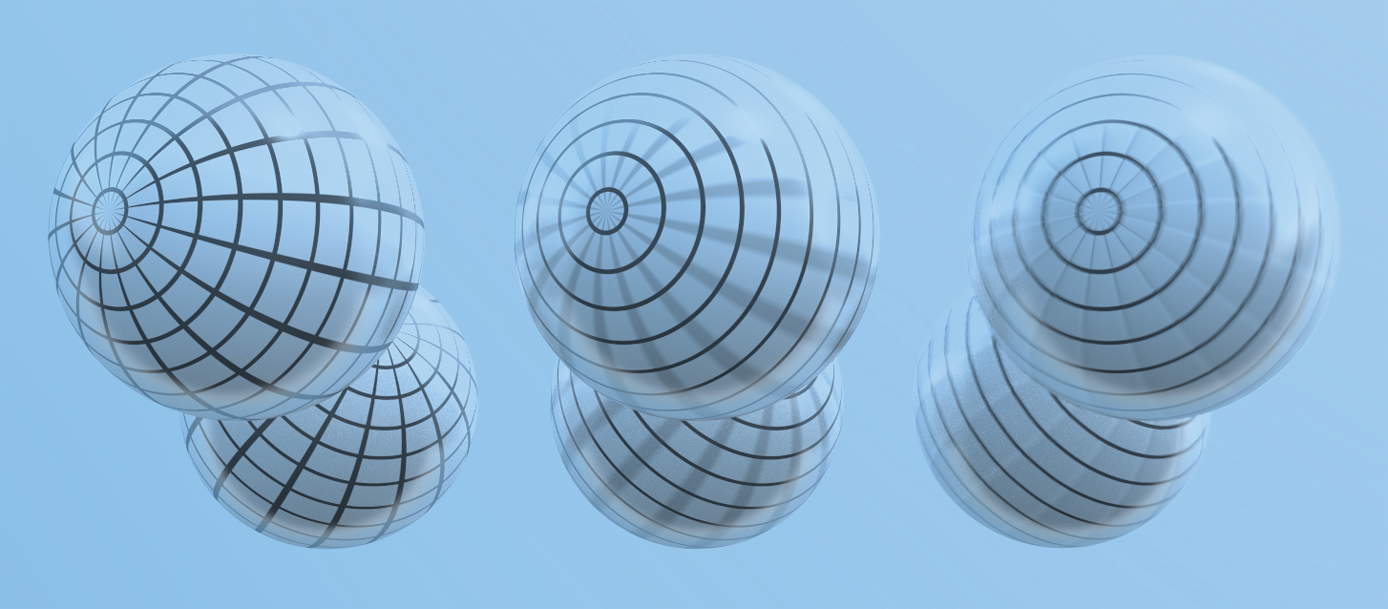
\includegraphics[width=\linewidth]{chap02/spinningspheres.png}
    \caption{转动的球体。用本节实现的变换动画代码以不同速率旋转三个球体并被镜子反射。
        注意球体的反射和球体自身一样模糊。}
    \label{fig:2.15}
\end{figure}

pbrt为场景中的相机和几何图元支持关键帧矩阵动画。
不只是提供单个变换放置场景中的相应物体,
用户还可能提供许多\keyindex{关键帧}{keyframe}{}变换,
每个都与特定时间点关联。
这能让相机移动起来并在仿真相机快门打开时让场景中的物体也移动起来。
\reffig{2.15}展示了三个运用pbrt关键帧矩阵动画的运动球体。

通常,在关键帧矩阵之间插值的问题是没有定义的。
例如,如果我们关于$x$轴旋转181度后再旋转181度,
这代表2度的小旋转还是-358度的大旋转?
再例如,考虑两个矩阵,一个是恒等的另一个是绕$z$轴旋转180度。
从其中一个到另一个有无数种方式可走。

关键帧矩阵插值在计算机动画中是一个重要的问题,
有许多不同的方法被开发出来。
幸运的是,有两个原因使得渲染器中的矩阵插值问题一般不像动画系统中的那么难。

首先,在一个像pbrt那样的渲染器中,
我们一般有分别在相机快门打开和关闭时的关键帧矩阵;
我们只需要在单张图像的时段里在两者之间插值。
在动画系统中,矩阵一般按更低的时间频率提供,
所以一对关键帧矩阵之间有许多帧;
这样,就有更多机会注意到插值中的问题。

第二,在基于物理的渲染器中,需要我们插值的矩阵对的时段越长,
虚拟相机快门就打开得越久,最终图像的运动模糊就越多;
运动模糊的增加常常隐藏了插值的缺点。

对由关键帧矩阵定义的变换最简单的插值方法——
直接对矩阵的每个分量插值——并不是一个好办法,因为它一般会导致意外不良结果。
例如,如果变换应用了不同的旋转,则即使是刚体运动,中间的矩阵也可能缩放物体,这明显不是我们期望的。
(如果矩阵在它们之间有完整180度的旋转,则插值的中间物体可能缩小到不见!)

\reffig{2.16}展示了在该帧过程中旋转90度的球体;
直接对矩阵元素插值给出的结果不如本节实现的方法准确。
\begin{figure}[htbp]
    \raggedright
    \subfloat[静止球体。]{\label{fig:2.16.1}
\includegraphics[width=0.5\linewidth]{chap02/sphere-still.png}}%
    \subfloat[旋转,正确插值。]{\label{fig:2.16.2}
\includegraphics[width=0.5\linewidth]{chap02/sphere-rot-good.png}}\\%
    \subfloat[旋转,错误插值。]{\label{fig:2.16.3}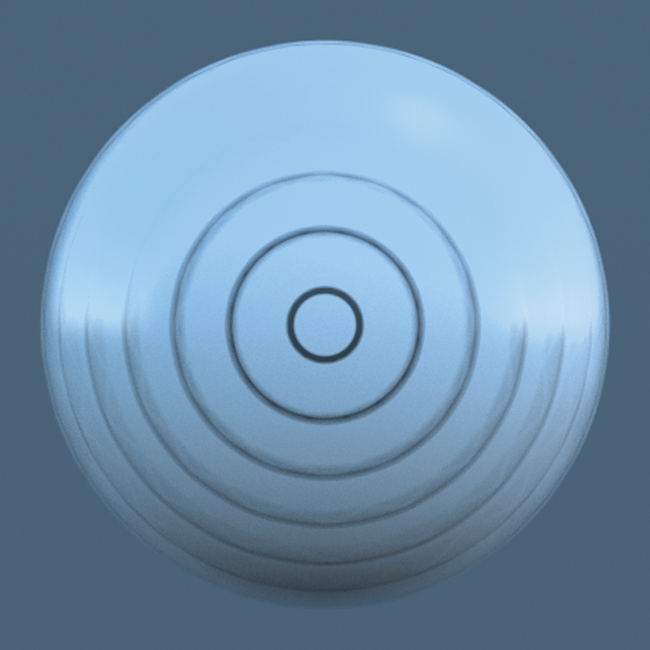
\includegraphics[width=0.5\linewidth]{chap02/sphere-rot-bad.png}}\quad%
    \begin{minipage}{0.45\textwidth}
        \vspace{-\linewidth}\caption{变换插值错误的影响。(a)球体以网格线作为纹理,没有旋转。
            (b)球体在该帧过程中旋转90度,使用本节实现的变换插值技术。
            (c)球体旋转90度,直接对矩阵分量插值来对变换插值。
            这时,动画球体错误地变大了并且靠球体外本应清晰的线条也错误地变模糊了。}
        \label{fig:2.16}
    \end{minipage}
\end{figure}

pbrt中使用的变换插值方法是基于\keyindex{矩阵分解}{matrix decomposition}{}——
给定任意变换矩阵$\bm M$,我们将其分解为
缩放($\bm S$)、旋转($\bm R$)和平移($\bm T$)变换的级联,
\begin{align*}
    \bm M=\bm S\bm R\bm T\, ,
\end{align*}
其中这些分量每一个都是独立插值,然后合成的插值矩阵由三个插值矩阵一起相乘得到。

{\noindent\hfil$=========$\hfil{\color{red}{施工分割线}}\hfil$=========$\
\section{交互作用}\label{sec:交互作用}

\begin{lstlisting}
`\initcode{Interaction Declarations}{=}\initnext{InteractionDeclarations}`
struct `\initvar{Interaction}{}` {
    `\refcode{Interaction Public Methods}{}`
    `\refcode{Interaction Public Data}{}`
};
\end{lstlisting}

\begin{lstlisting}
`\initcode{Interaction Public Data}{=}\initnext{InteractionPublicData}`
`\refvar{Point3f}{}` `\initvar[Interaction::p]{p}{}`;
Float `\initvar[Interaction::time]{time}{}`;
\end{lstlisting}

\begin{lstlisting}
`\refcode{Interaction Public Data}{+=}\lastnext{InteractionPublicData}`
`\refvar{Vector3f}{}` `\initvar{pError}{}`;
\end{lstlisting}

\begin{lstlisting}
`\refcode{Interaction Public Data}{+=}\lastnext{InteractionPublicData}`
`\refvar{Vector3f}{}` `\initvar[Interaction::wo]{wo}{}`;
\end{lstlisting}

\begin{lstlisting}
`\refcode{Interaction Public Data}{+=}\lastnext{InteractionPublicData}`
`\refvar{Normal3f}{}` `\initvar[Interaction::n]{n}{}`;
\end{lstlisting}

\subsection{表面交互}\label{sub:表面交互}
\begin{lstlisting}
`\initcode{SurfaceInteraction Declarations}{=}`
class `\initvar{SurfaceInteraction}{}` : public `\refvar{Interaction}{}` {
public:
    `\refcode{SurfaceInteraction Public Methods}{}`
    `\refcode{SurfaceInteraction Public Data}{}`
};
\end{lstlisting}

\begin{lstlisting}
`\initcode{SurfaceInteraction Public Data}{=}\initnext{SurfaceInteractionPublicData}`
`\refvar{Point2f}{}` `\initvar[SurfaceInteraction::uv]{uv}{}`;
`\refvar{Vector3f}{}` `\initvar[SurfaceInteraction::dpdu]{dpdu}{}`, `\initvar[SurfaceInteraction::dpdv]{dpdv}{}`;
`\refvar{Normal3f}{}` `\initvar[SurfaceInteraction::dndu]{dndu}{}`, `\initvar[SurfaceInteraction::dndv]{dndv}{}`;
const `\refvar{Shape}{}` *`\initvar{shape}{}` = nullptr;
\end{lstlisting}

\begin{lstlisting}
`\initcode{SurfaceInteraction Method Definitions}{=}\initnext{SurfaceInteractionMethodDefinitions}`
`\refvar{SurfaceInteraction}{}`::`\refvar{SurfaceInteraction}{}`(const `\refvar{Point3f}{}` &p,
    const `\refvar{Vector3f}{}` &pError, const `\refvar{Point2f}{}` &uv, const `\refvar{Vector3f}{}` &wo,
    const `\refvar{Vector3f}{}` &dpdu, const `\refvar{Vector3f}{}` &dpdv,
    const `\refvar{Normal3f}{}` &dndu, const `\refvar{Normal3f}{}` &dndv,
    Float time, const `\refvar{Shape}{}` *shape)
    : `\refvar{Interaction}{}`(p, `\refvar{Normal3f}{}`(`\refvar{Normalize}{}`(`\refvar{Cross}{}`(dpdu, dpdv))), pError, wo,
    time, nullptr),
    `\refvar[SurfaceInteraction::uv]{uv}{}`(uv), `\refvar[SurfaceInteraction::dpdu]{dpdu}{}`(dpdu), `\refvar[SurfaceInteraction::dpdv]{dpdv}{}`(dpdv), `\refvar[SurfaceInteraction::dndu]{dndu}{}`(dndu), `\refvar[SurfaceInteraction::dndv]{dndv}{}`(dndv),
    `\refvar{shape}{}`(shape) {
    `\refcode{Initialize shading geometry from true geometry}{}`
    `\refcode{Adjust normal based on orientation and handedness}{}`
}
\end{lstlisting}

\begin{lstlisting}
`\refcode{SurfaceInteraction Public Data}{+=}\lastnext{SurfaceInteractionPublicData}`
struct {
    `\refvar{Normal3f}{}` `\initvar[shading::n]{n}{}`;
    `\refvar{Vector3f}{}` `\initvar[shading::dpdu]{dpdu}{}`, `\initvar[shading::dpdv]{dpdv}{}`;
    `\refvar{Normal3f}{}` `\initvar[shading::dndu]{dndu}{}`, `\initvar[shading::dndv]{dndv}{}`;
} `\initvar{shading}{}`;
\end{lstlisting}

\section{译者补充:四元数}\label{sec:译者补充:四元数}
\begin{remark}
    本节内容不是原书内容,而是译者自学补充的,请酌情参考和斧正。
\end{remark}

本节内容主要依据文献\citep{10.5555/90767.90913,enwiki:1013104981}整理而成,
给出四元数相关数学推导,具体介绍
四元数的定义、性质及其在几何变换中的运用。

\subsection{四元数的定义}\label{sub:四元数的定义}
\begin{definition}
    \keyindex{四元数}{quaternion}{}记作
    \begin{align}
        {\bm q}=w+x\mathbf{i}+y\mathbf{j}+z\mathbf{k}\, ,
    \end{align}
    其中$w, x, y, z$是实数,
    $\mathbf{i}, \mathbf{j}, \mathbf{k}$是\keyindex{基四元数}{basic quaternion}{quaternion四元数},
    也称\keyindex{基元}{basis element}{quaternion四元数}。

    基四元数可视为分别指向三个空间轴向的单位向量。
    此时${\bm q}$可视作由一个标量和一个向量构成:
    其中$w$称为\keyindex{实部}{real part}{}或\keyindex{标量部}{scalar part}{quaternion四元数},
    $x\mathbf{i}+y\mathbf{j}+z\mathbf{k}$称为\keyindex{虚部}{imaginary part}{quaternion四元数}、\keyindex{纯部}{pure part}{quaternion四元数}或\keyindex{向量部}{vector part}{quaternion四元数}。
\end{definition}
\begin{definition}
    当$w=0$且$xyz\neq 0$时,${\bm q}$称为\keyindex{向量四元数}{vector quaternion}{quaternion四元数}。
\end{definition}
\begin{definition}
    当$x=y=z=0$时,${\bm q}$称为\keyindex{标量四元数}{scalar quaternion}{quaternion四元数}。
    其中,当$w=x=y=z=0$时,${\bm q}$称为\keyindex{零四元数}{zero quaternion}{quaternion四元数},记作$0$。
\end{definition}
\begin{notation}
    在实际书写时,我们做如下约定
    \protect\sidenote{因为实数域$\mathbb{R}$、向量空间$\mathbb{R}^3$分别
        与$\mathbb{H}$的子集\protect\keyindex{同构}{isomorphic}{},
        所以即便在这种记法下
        实数与标量四元数、三维向量与向量四元数记号一样,
        其逻辑也是自洽的。}:
    \begin{itemize}
        \item $w, x, y, z$之一等于$0$时,略写相应项;
        \item $x, y, z$之一等于$1$时,相应项简写为$\mathbf{i, j}$或$\mathbf{k}$;
        \item 也可写作${\bm q}=w+{\bm u}$,其中$w$为标量,${\bm u}=x\mathbf{i}+y\mathbf{j}+z\mathbf{k}$为向量;
        \item 所有四元数构成的集合记作$\mathbb{H}$。
    \end{itemize}
\end{notation}


\subsection{四元数的运算}\label{sub:四元数的运算}
分别记四元数为
\begin{align}
    {\bm q}   & =w+{\bm u}=w+x\mathbf{i}+y\mathbf{j}+z\mathbf{k}\, ,             \\
    {\bm q}_n & =w_n+{\bm u}_n=w_n+x_n\mathbf{i}+y_n\mathbf{j}+z_n\mathbf{k}\, ,
\end{align}
其中$w, x, y, z, w_n, x_n, y_n, z_n\in\mathbb{R}$,${\bm u}, {\bm u}_n\in\mathbb{R}^3$,$n$为下标。
\begin{definition}
    四元数\keyindex{加法}{addition}{}为
    \begin{align}
        {\bm q}_1+{\bm q}_2 & =(w_1+w_2)+({\bm u}_1+{\bm u}_2)\nonumber                                  \\
                            & =(w_1+w_2)+(x_1+x_2)\mathbf{i}+(y_1+y_2)\mathbf{j}+(z_1+z_2)\mathbf{k}\, .
    \end{align}
\end{definition}
\begin{proposition}
    四元数加法的\keyindex{单位元}{identity element}{}是零四元数。
\end{proposition}
\begin{proposition}
    四元数加法的\keyindex{逆元}{inverse element}{}是
    \begin{align}
        -{\bm q}=-w-x\mathbf{i}-y\mathbf{j}-z\mathbf{k}\, .
    \end{align}
\end{proposition}
\begin{proposition}
    四元数的加法满足\keyindex{交换律}{law of commutation}{}
    \begin{align}
        {\bm q}_1+{\bm q}_2={\bm q}_2+{\bm q}_1, \quad \forall {\bm q}_1, {\bm q}_2\in \mathbb{H}\, .
    \end{align}
\end{proposition}
\begin{proposition}
    四元数的加法满足\keyindex{结合律}{law of association}{}
    \begin{align}
        ({\bm q}_1+{\bm q}_2)+{\bm q}_3={\bm q}_1+({\bm q}_2+{\bm q}_3), \quad \forall {\bm q}_1, {\bm q}_2, {\bm q}_3\in \mathbb{H}\, .
    \end{align}
\end{proposition}
\begin{notation}
    约定向量的\keyindex{数乘}{scalar multiplication}{}、\keyindex{内积}{inner product}{}、\keyindex{叉积}{cross product}{}分别记作
    \begin{align}
        \lambda{\bm u}           & =(\lambda x)\mathbf{i}+(\lambda y)\mathbf{j}+(\lambda z)\mathbf{k},\quad \forall \lambda\in\mathbb{R}\, , \\
        {\bm u}_1\cdot{\bm u}_2  & =x_1x_2+y_1y_2+z_1z_2\, ,                                                                                 \\
        {\bm u}_1\times{\bm u}_2 & =(y_1z_2-y_2z_1)\mathbf{i}+(z_1x_2-z_2x_1)\mathbf{j}+(x_1y_2-x_2y_1)\mathbf{k}\, .
    \end{align}
\end{notation}
\begin{definition}
    四元数${\bm q}$与实数$\lambda$的\keyindex{数乘}{scalar multiplication}{}为
    \begin{align}
        \lambda{\bm q}={\bm q}\lambda & =\lambda w+\lambda {\bm u}\nonumber                                              \\
                                      & =\lambda w+(\lambda x)\mathbf{i}+(\lambda y)\mathbf{j}+(\lambda z)\mathbf{k}\, .
    \end{align}
\end{definition}
\begin{proposition}
    四元数的数乘对加法满足\keyindex{分配律}{law of distribution}{}
    \begin{align}
        (\lambda_1+\lambda_2){\bm q} & =\lambda_1{\bm q}+\lambda_2{\bm q}, \quad \forall \lambda_1, \lambda_2\in\mathbb{R}, \forall {\bm q}\in\mathbb{H}\, , \\
        \lambda({\bm q}_1+{\bm q}_2) & =\lambda{\bm q}_1+\lambda{\bm q}_2, \quad \forall \lambda\in\mathbb{R}, \forall {\bm q}_1, {\bm q}_2\in\mathbb{H}\, .
    \end{align}
\end{proposition}
\begin{definition}
    基元$\mathbf{i}, \mathbf{j}, \mathbf{k}$的乘法为
    \begin{align}
        1\mathbf{i}  & =\mathbf{i}1=\mathbf{i}, & 1\mathbf{j}  & =\mathbf{j}1=\mathbf{j}, & 1\mathbf{k}  & =\mathbf{k}1=\mathbf{k}\, ,\nonumber \\
        \mathbf{i}^2 & =-1,                     & \mathbf{j}^2 & =-1,                     & \mathbf{k}^2 & =-1\, ,                    \nonumber \\
        \mathbf{ij}  & =\mathbf{k},             & \mathbf{jk}  & =\mathbf{i},             & \mathbf{ki}  & =\mathbf{j}\, ,            \nonumber \\
        \mathbf{ji}  & =-\mathbf{k},            & \mathbf{kj}  & =-\mathbf{i},            & \mathbf{ik}  & =-\mathbf{j}\, .
    \end{align}
\end{definition}
\begin{definition}
    四元数\keyindex{乘法}{multiplication}{}为
    \begin{align}
        {\bm q}_1{\bm q}_2 & =(w_1+{\bm u}_1)(w_2+{\bm u}_2)\nonumber                                                                      \\
                           & =(w_1+x_1\mathbf{i}+y_1\mathbf{j}+z_1\mathbf{k})(w_2+x_2\mathbf{i}+y_2\mathbf{j}+z_2\mathbf{k})\nonumber      \\
                           & =\quad w_1w_2+w_1x_2\mathbf{i}+w_1y_2\mathbf{j}+w_1z_2\mathbf{k}\nonumber                                     \\
                           & \quad +x_1w_2\mathbf{i}+x_1x_2\mathbf{i}^2+x_1y_2\mathbf{i}\mathbf{j}+x_1z_2\mathbf{i}\mathbf{k}\nonumber     \\
                           & \quad +y_1w_2\mathbf{j}+y_1x_2\mathbf{j}\mathbf{i}+y_1y_2\mathbf{j}^2+y_1z_2\mathbf{j}\mathbf{k}\nonumber     \\
                           & \quad +z_1w_2\mathbf{k}+z_1x_2\mathbf{k}\mathbf{i}+z_1y_2\mathbf{k}\mathbf{j}+z_1z_2\mathbf{k}^2\nonumber     \\
                           & =\quad w_1w_2-(x_1x_2+y_1y_2+z_1z_2)\nonumber                                                                 \\
                           & \quad +w_1(x_2\mathbf{i}+y_2\mathbf{j}+z_2\mathbf{k})+w_2(x_1\mathbf{i}+y_1\mathbf{j}+z_1\mathbf{k})\nonumber \\
                           & \quad +(y_1z_2-y_2z_1)\mathbf{i}+(z_1x_2-z_2x_1)\mathbf{j}+(x_1y_2-x_2y_1)\mathbf{k}\nonumber                 \\
                           & =(w_1w_2-{\bm u}_1\cdot{\bm u}_2)+(w_1{\bm u}_2+w_2{\bm u}_1+{\bm u}_1\times{\bm u}_2)\, ,
    \end{align}
    也称为\keyindex{哈密顿积}{Hamilton product}{}。
\end{definition}
\begin{proposition}
    四元数乘法的单位元是$1$。
\end{proposition}
\begin{corollary}
    四元数的乘法不满足交换律。
\end{corollary}
\begin{example}
    取
    \begin{align}
        {\bm q}_1 & =1+2\mathbf{i}+3\mathbf{j}+4\mathbf{k}\, , \\
        {\bm q}_2 & =5+6\mathbf{i}+7\mathbf{j}+8\mathbf{k}\, .
    \end{align}
    于是易得
    \begin{align}
        {\bm q}_1{\bm q}_2 & =-60+12\mathbf{i}+30\mathbf{j}+24\mathbf{k}\, , \\
        {\bm q}_2{\bm q}_1 & =-60+20\mathbf{i}+14\mathbf{j}+32\mathbf{k}\, .
    \end{align}
    显然${\bm q}_1{\bm q}_2\neq{\bm q}_2{\bm q}_1$。
\end{example}
\begin{proposition}
    四元数的乘法满足结合律
    \begin{align}
        ({\bm q}_1{\bm q}_2){\bm q}_3={\bm q}_1({\bm q}_2{\bm q}_3), \quad \forall {\bm q}_1, {\bm q}_2, {\bm q}_3\in \mathbb{H}\, .
    \end{align}
\end{proposition}
\begin{prove}
    根据定义有
    \begin{align}
        ({\bm q}_1{\bm q}_2){\bm q}_3 & =((w_1+{\bm u}_1)(w_2+{\bm u}_2))(w_3+{\bm u}_3)\nonumber                                                                                           \\
                                      & =((w_1w_2-{\bm u}_1\cdot{\bm u}_2)+(w_1{\bm u}_2+w_2{\bm u}_1+{\bm u}_1\times{\bm u}_2))(w_3+{\bm u}_3)\nonumber                                    \\
                                      & =\quad ((w_1w_2-{\bm u}_1\cdot{\bm u}_2)w_3-(w_1{\bm u}_2+w_2{\bm u}_1+{\bm u}_1\times{\bm u}_2)\cdot{\bm u}_3)\nonumber                            \\
                                      & \quad +((w_1w_2-{\bm u}_1\cdot{\bm u}_2){\bm u}_3+w_3(w_1{\bm u}_2+w_2{\bm u}_1+{\bm u}_1\times{\bm u}_2)\nonumber                                  \\
                                      & \quad +(w_1{\bm u}_2+w_2{\bm u}_1+{\bm u}_1\times{\bm u}_2)\times{\bm u}_3)\nonumber                                                                \\
                                      & =\quad w_1w_2w_3-w_3{\bm u}_1\cdot{\bm u}_2-w_1{\bm u}_2\cdot{\bm u}_3-w_2{\bm u}_1\cdot{\bm u}_3-({\bm u}_1\times{\bm u}_2)\cdot{\bm u}_3\nonumber \\
                                      & \quad +w_1w_2{\bm u}_3-({\bm u}_1\cdot{\bm u}_2){\bm u}_3+w_3w_1{\bm u}_2+w_2w_3{\bm u}_1+w_3{\bm u}_1\times{\bm u}_2\nonumber                      \\
                                      & \quad +w_1{\bm u}_2\times{\bm u}_3+w_2{\bm u}_1\times{\bm u}_3+({\bm u}_1\times{\bm u}_2)\times{\bm u}_3\nonumber                                   \\
                                      & =\quad  w_1w_2w_3-({\bm u}_1\times{\bm u}_2)\cdot{\bm u}_3+({\bm u}_1\times{\bm u}_2)\times{\bm u}_3-({\bm u}_1\cdot{\bm u}_2){\bm u}_3\nonumber    \\
                                      & \quad +w_2w_3{\bm u}_1+w_1{\bm u}_2\times{\bm u}_3-w_1{\bm u}_2\cdot{\bm u}_3\nonumber                                                              \\
                                      & \quad +w_3w_1{\bm u}_2+w_2{\bm u}_1\times{\bm u}_3-w_2{\bm u}_1\cdot{\bm u}_3\nonumber                                                              \\
                                      & \quad +w_1w_2{\bm u}_3+w_3{\bm u}_1\times{\bm u}_2-w_3{\bm u}_1\cdot{\bm u}_2\, .
    \end{align}
    同理有
    \begin{align}
        {\bm q}_1({\bm q}_2{\bm q}_3) & =(w_1+{\bm u}_1)((w_2+{\bm u}_2)(w_3+{\bm u}_3))\nonumber                                                                                           \\
                                      & =(w_1+{\bm u}_1)((w_2w_3-{\bm u}_2\cdot{\bm u}_3)+(w_2{\bm u}_3+w_3{\bm u}_2+{\bm u}_2\times{\bm u}_3))\nonumber                                    \\
                                      & =\quad(w_1(w_2w_3-{\bm u}_2\cdot{\bm u}_3)-{\bm u}_1\cdot(w_2{\bm u}_3+w_3{\bm u}_2+{\bm u}_2\times{\bm u}_3))\nonumber                             \\
                                      & \quad +(w_1(w_2{\bm u}_3+w_3{\bm u}_2+{\bm u}_2\times{\bm u}_3)+(w_2w_3-{\bm u}_2\cdot{\bm u}_3){\bm u}_1\nonumber                                  \\
                                      & \quad +{\bm u}_1\times(w_2{\bm u}_3+w_3{\bm u}_2+{\bm u}_2\times{\bm u}_3))\nonumber                                                                \\
                                      & =\quad w_1w_2w_3-w_1{\bm u}_2\cdot{\bm u}_3-w_2{\bm u}_1\cdot{\bm u}_3-w_3{\bm u}_1\cdot{\bm u}_2-{\bm u}_1\cdot({\bm u}_2\times{\bm u}_3)\nonumber \\
                                      & \quad +w_1w_2{\bm u}_3+w_1w_3{\bm u}_2+w_1{\bm u}_2\times{\bm u}_3+w_2w_3{\bm u}_1-({\bm u}_2\cdot{\bm u}_3){\bm u}_1\nonumber                      \\
                                      & \quad +w_2{\bm u}_1\times{\bm u}_3+w_3{\bm u}_1\times{\bm u}_2+{\bm u}_1\times({\bm u}_2\times{\bm u}_3)\nonumber                                   \\
                                      & =\quad w_1w_2w_3-{\bm u}_1\cdot({\bm u}_2\times{\bm u}_3)+{\bm u}_1\times({\bm u}_2\times{\bm u}_3)-({\bm u}_2\cdot{\bm u}_3){\bm u}_1\nonumber     \\
                                      & \quad +w_2w_3{\bm u}_1+w_1{\bm u}_2\times{\bm u}_3-w_1{\bm u}_2\cdot{\bm u}_3\nonumber                                                              \\
                                      & \quad +w_3w_1{\bm u}_2+w_2{\bm u}_1\times{\bm u}_3-w_2{\bm u}_1\cdot{\bm u}_3\nonumber                                                              \\
                                      & \quad +w_1w_2{\bm u}_3+w_3{\bm u}_1\times{\bm u}_2-w_3{\bm u}_1\cdot{\bm u}_2\, .
    \end{align}
    注意到向量运算有\sidenote{它们其实是向量的\protect\keyindex{标量三重积}{scalar triple product}{}的两种等价定义,也称\protect\keyindex{混合积}{mixed product}{}。}
    \begin{align}
        ({\bm u}_1\times{\bm u}_2)\cdot{\bm u}_3\equiv{\bm u}_1\cdot({\bm u}_2\times{\bm u}_3)\, ,
    \end{align}
    以及\sidenote{第一个和第三个等号的变换利用了\protect\keyindex{向量三重积}{vector triple product}{}的性质,
        也称为\protect\keyindex{三重积展开}{triple product expansion}{}或\protect\keyindex{拉格朗日公式}{Lagrange's formula}{}。}
    \begin{align}
          & ({\bm u}_1\times{\bm u}_2)\times{\bm u}_3-({\bm u}_1\cdot{\bm u}_2){\bm u}_3\nonumber                             \\
        = & ({\bm u}_1\cdot{\bm u}_3){\bm u}_2-({\bm u}_2\cdot{\bm u}_3){\bm u}_1-({\bm u}_1\cdot{\bm u}_2){\bm u}_3\nonumber \\
        = & ({\bm u}_1\cdot{\bm u}_3){\bm u}_2-({\bm u}_1\cdot{\bm u}_2){\bm u}_3-({\bm u}_2\cdot{\bm u}_3){\bm u}_1\nonumber \\
        = & ({\bm u}_3\times{\bm u}_2)\times{\bm u}_1-({\bm u}_2\cdot{\bm u}_3){\bm u}_1\nonumber                             \\
        = & {\bm u}_1\times(-{\bm u}_3\times{\bm u}_2)-({\bm u}_2\cdot{\bm u}_3){\bm u}_1\nonumber                            \\
        = & {\bm u}_1\times({\bm u}_2\times{\bm u}_3)-({\bm u}_2\cdot{\bm u}_3){\bm u}_1\, .
    \end{align}
    所以$({\bm q}_1{\bm q}_2){\bm q}_3={\bm q}_1({\bm q}_2{\bm q}_3)$成立。
\end{prove}
\begin{proposition}
    四元数的乘法对加法满足分配律
    \begin{align}
        {\bm q}_1({\bm q}_2+{\bm q}_3)={\bm q}_1{\bm q}_2+{\bm q}_1{\bm q}_3, \quad \forall {\bm q}_1, {\bm q}_2, {\bm q}_3\in \mathbb{H}\, , \\
        ({\bm q}_1+{\bm q}_2){\bm q}_3={\bm q}_1{\bm q}_3+{\bm q}_2{\bm q}_3, \quad \forall {\bm q}_1, {\bm q}_2, {\bm q}_3\in \mathbb{H}\, .
    \end{align}
\end{proposition}
\begin{prove}
    根据定义有
    \begin{align}
        {\bm q}_1({\bm q}_2+{\bm q}_3) & =(w_1+{\bm u}_1)((w_2+{\bm u}_2)+(w_3+{\bm u}_3))\nonumber                                            \\
                                       & =(w_1+{\bm u}_1)((w_2+w_3)+({\bm u}_2+{\bm u}_3))\nonumber                                            \\
                                       & =\quad (w_1(w_2+w_3)-{\bm u}_1\cdot({\bm u}_2+{\bm u}_3))\nonumber                                    \\
                                       & \quad +(w_1({\bm u}_2+{\bm u}_3)+(w_2+w_3){\bm u}_1+{\bm u}_1\times({\bm u}_2+{\bm u}_3))\nonumber    \\
                                       & =\quad (w_1w_2-{\bm u}_1\cdot{\bm u}_2)+(w_1{\bm u}_2+w_2{\bm u}_1+{\bm u}_1\times{\bm u}_2)\nonumber \\
                                       & \quad +(w_1w_3-{\bm u}_1\cdot{\bm u}_3)+(w_1{\bm u}_3+w_3{\bm u}_1{\bm u}_1\times{\bm u}_3)\nonumber  \\
                                       & ={\bm q}_1{\bm q}_2+{\bm q}_1{\bm q}_3\, .
    \end{align}
    \begin{align}
        ({\bm q}_1+{\bm q}_2){\bm q}_3 & =((w_1+{\bm u}_1)+(w_2+{\bm u}_2))(w_3+{\bm u}_3)\nonumber                                            \\
                                       & =((w_1+w_2)+({\bm u}_1+{\bm u}_2))(w_3+{\bm u}_3)\nonumber                                            \\
                                       & =\quad ((w_1+w_2)w_3-({\bm u}_1+{\bm u}_2)\cdot{\bm u}_3)\nonumber                                    \\
                                       & \quad +((w_1+w_2){\bm u}_3+w_3({\bm u}_1+{\bm u}_2)+({\bm u}_1+{\bm u}_2)\times{\bm u}_3)\nonumber    \\
                                       & =\quad (w_1w_3-{\bm u}_1\cdot{\bm u}_3)+(w_1{\bm u}_3+w_3{\bm u}_1+{\bm u}_1\times{\bm u}_3)\nonumber \\
                                       & \quad +(w_2w_3-{\bm u}_2\cdot{\bm u}_3)+(w_2{\bm u}_3+w_3{\bm u}_2+{\bm u}_2\times{\bm u}_3)\nonumber \\
                                       & ={\bm q}_1{\bm q}_3+{\bm q}_2{\bm q}_3\, .
    \end{align}
\end{prove}
\begin{definition}
    称四元数${\bm q}=w+{\bm u}$与$\bar{\bm q}=w-{\bm u}$互为\keyindex{共轭}{conjugate}{}。
\end{definition}
\begin{proposition}
    四元数积的共轭等于逆序共轭的积,即
    \begin{align}
        \overline{{\bm q}_1{\bm q}_2}=\bar{\bm q}_2\bar{\bm q}_1, \quad\forall {\bm q}_1, {\bm q}_2\in\mathbb{H}\, .
    \end{align}
\end{proposition}
\begin{prove}
    根据定义有
    \begin{align}
        \overline{{\bm q}_1{\bm q}_2} & =(w_1w_2-{\bm u}_1\cdot{\bm u}_2)-(w_1{\bm u}_2+w_2{\bm u}_1+{\bm u}_1\times{\bm u}_2)\nonumber                   \\
                                      & =(w_2w_1-(-{\bm u}_2)\cdot(-{\bm u}_1))+(w_2(-{\bm u}_1)+w_1(-{\bm u}_2)+(-{\bm u}_2)\times(-{\bm u}_1))\nonumber \\
                                      & =(w_2-{\bm u}_2)(w_1-{\bm u}_1)\nonumber                                                                          \\
                                      & =\bar{\bm q}_2\bar{\bm q}_1\, .
    \end{align}
\end{prove}
\begin{definition}
    四元数的\keyindex{模}{magnitude}{}为
    \begin{align}
        \|{\bm q}\|=\sqrt{{\bm q}\bar{\bm q}}=\sqrt{\bar{\bm q}{\bm q}}=\sqrt{w^2+x^2+y^2+z^2}\, .
    \end{align}
\end{definition}
\begin{definition}
    模为$1$的四元数${\bm q}$称为\keyindex{单位四元数}{unit quaternion}{quaternion四元数}。
\end{definition}
\begin{definition}
    称$、\displaystyle\frac{1}{\|{\bm q}\|}{\bm q}$为非零四元数${\bm q}$的\keyindex{规范化四元数}{versor}{quaternion四元数}。
\end{definition}
\begin{proposition}
    当向量四元数${\bm q}$是单位四元数即$w=0$且$x^2+y^2+z^2=1$时,有
    \begin{align}
        {\bm q}^2={\bm q}{\bm q}=-1\, .
    \end{align}
\end{proposition}
\begin{prove}
    依据哈密顿积定义有
    \begin{align}
        {\bm q}^2={\bm q}{\bm q} & =(w^2-{\bm u}\cdot{\bm u})+(2c{\bm u}+{\bm u}\times{\bm u})\nonumber \\
                                 & =-{\bm u}\cdot{\bm u}\nonumber                                       \\
                                 & =-(x^2+y^2+z^2)\nonumber                                             \\
                                 & =-1\, .
    \end{align}
\end{prove}
\begin{proposition}
    四元数取共轭后模不变,即
    \begin{align}
        \|\bar{\bm q}\|=\|{\bm q}\|\, .
    \end{align}
\end{proposition}
\begin{proposition}
    在四元数的数乘中有
    \begin{align}
        \|\lambda{\bm q}\|=|\lambda|\|{\bm q}\|, \quad \forall \lambda\in\mathbb{R}, \forall {\bm q}\in\mathbb{H}\, .
    \end{align}
\end{proposition}
\begin{proposition}
    在四元数的乘法中有
    \begin{align}
        \|{\bm q}_1{\bm q}_2\|=\|{\bm q}_1\|\|{\bm q}_2\|,\quad \forall {\bm q}_1{\bm q}_2\in\mathbb{H}\, .
    \end{align}
\end{proposition}
\begin{prove}
    根据定义可得
    \begin{align}
        \|{\bm q}_1{\bm q}_2\|^2 = & \|(w_1w_2-x_1x_2-y_1y_2-z_1z_2)\nonumber                    \\
                                   & +(w_1x_2+w_2x_1+y_1z_2-y_2z_1)\mathbf{i}\nonumber           \\
                                   & +(w_1y_2+w_2y_1+z_1x_2-z_2x_1)\mathbf{j}\nonumber           \\
                                   & +(w_1z_2+w_2z_1+x_1y_2-x_2y_1)\mathbf{k}\|^2\nonumber       \\
        =                          & (w_1w_2-x_1x_2-y_1y_2-z_1z_2)^2\nonumber                    \\
                                   & +(w_1x_2+w_2x_1+y_1z_2-y_2z_1)^2\nonumber                   \\
                                   & +(w_1y_2+w_2y_1+z_1x_2-z_2x_1)^2\nonumber                   \\
                                   & +(w_1z_2+w_2z_1+x_1y_2-x_2y_1)^2\nonumber                   \\
        =                          & (w_1^2+x_1^2+y_1^2+z_1^2)(w_2^2+x_2^2+y_2^2+z_2^2)\nonumber \\
        =                          & \|{\bm q}_1\|^2\|{\bm q}_2\|^2\, ,
    \end{align}
    所以$\|{\bm q}_1{\bm q}_2\|=\|{\bm q}_1\|\|{\bm q}_2\|$。
\end{prove}

\begin{proposition}
    四元数${\bm q}$与其共轭的积恒有
    \begin{align}
        {\bm q}\bar{\bm q}=\bar{\bm q}{\bm q}=\|{\bm q}\|^2\, .
    \end{align}
\end{proposition}
\begin{prove}
    根据定义有
    \begin{align}
        {\bm q}\bar{\bm q} & =(w+{\bm u})(w-{\bm u})\nonumber                                                      \\
                           & =(w^2-{\bm u}\cdot(-{\bm u}))+(w(-{\bm u})+w{\bm u}+{\bm u}\times(-{\bm u}))\nonumber \\
                           & =w^2+{\bm u}\cdot{\bm u}\nonumber                                                     \\
                           & =\|{\bm q}\|^2\, .
    \end{align}
    同理有$\bar{\bm q}{\bm q}=\|{\bm q}\|^2$。
\end{prove}
\begin{definition}
    非零四元数${\bm q}$的\keyindex{逆}{inverse}{}是
    \begin{align}
        {\bm q}^{-1}=\frac{1}{\|{\bm q}\|^2}\bar{\bm q}\, .
    \end{align}
    它是哈密顿积的逆元。
\end{definition}
\begin{corollary}
    对于非零四元数${\bm q}$有
    \begin{align}
        {\bm q}{\bm q}^{-1}={\bm q}^{-1}{\bm q}=1\, .
    \end{align}
\end{corollary}
\begin{corollary}
    单位四元数的逆与共轭相等,即
    \begin{align}
        \|{\bm q}\|=1 \Rightarrow {\bm q}^{-1}=\bar{\bm q}\, .
    \end{align}
\end{corollary}

\subsection{四元数与旋转变换}\label{sub:四元数与旋转变换}
如\reffig{2.ex1}所示,点$P$绕单位向量$\bm n$给定的轴顺时针旋转角度$\theta$得到点$P'$。
我们现在说明该一般旋转变换和四元数运算的关系。
\begin{figure}[htbp]
    \centering%LaTeX with PSTricks extensions
%%Creator: Inkscape 1.0.1 (3bc2e813f5, 2020-09-07)
%%Please note this file requires PSTricks extensions
\psset{xunit=.25pt,yunit=.25pt,runit=.25pt}
\begin{pspicture}(438.27934686,472.27909118)
{
\newrgbcolor{curcolor}{0 0 0}
\pscustom[linewidth=4.04194013,linecolor=curcolor,linestyle=dashed,dash=6.41655016 2.13884997]
{
\newpath
\moveto(319.93053732,53.44303071)
\lineto(186.29461795,409.0229337)
}
}
{
\newrgbcolor{curcolor}{0 0 0}
\pscustom[linestyle=none,fillstyle=solid,fillcolor=curcolor]
{
\newpath
\moveto(191.98244641,393.88869807)
\lineto(202.39347846,389.16549449)
\lineto(184.87266084,412.80649261)
\lineto(187.25924283,383.47766603)
\closepath
}
}
{
\newrgbcolor{curcolor}{0 0 0}
\pscustom[linewidth=2.15570147,linecolor=curcolor]
{
\newpath
\moveto(191.98244641,393.88869807)
\lineto(202.39347846,389.16549449)
\lineto(184.87266084,412.80649261)
\lineto(187.25924283,383.47766603)
\closepath
}
}
{
\newrgbcolor{curcolor}{0 0 0}
\pscustom[linewidth=4.14531002,linecolor=curcolor]
{
\newpath
\moveto(184.55716913,413.7263252)
\lineto(411.21262866,413.7263252)
}
}
{
\newrgbcolor{curcolor}{0 0 0}
\pscustom[linestyle=none,fillstyle=solid,fillcolor=curcolor]
{
\newpath
\moveto(394.63138859,413.7263252)
\lineto(386.34076855,405.43570516)
\lineto(415.35793868,413.7263252)
\lineto(386.34076855,422.01694524)
\closepath
}
}
{
\newrgbcolor{curcolor}{0 0 0}
\pscustom[linewidth=2.21083208,linecolor=curcolor]
{
\newpath
\moveto(394.63138859,413.7263252)
\lineto(386.34076855,405.43570516)
\lineto(415.35793868,413.7263252)
\lineto(386.34076855,422.01694524)
\closepath
}
}
{
\newrgbcolor{curcolor}{0 0 0}
\pscustom[linewidth=4.11835988,linecolor=curcolor]
{
\newpath
\moveto(417.52037092,412.81663857)
\curveto(390.12953195,356.63810721)(335.92909659,307.69617224)(267.1004223,276.99036162)
\curveto(198.27174801,246.284551)(120.58876958,236.39072937)(51.51046353,249.53249838)
}
}
{
\newrgbcolor{curcolor}{0 0 0}
\pscustom[linewidth=4.33349279,linecolor=curcolor]
{
\newpath
\moveto(184.47597354,413.93886693)
\lineto(56.00338016,254.5407315)
}
}
{
\newrgbcolor{curcolor}{0 0 0}
\pscustom[linestyle=none,fillstyle=solid,fillcolor=curcolor]
{
\newpath
\moveto(66.88101129,268.03679377)
\lineto(65.57179572,280.22364048)
\lineto(53.28397237,251.16671593)
\lineto(79.067858,269.34600934)
\closepath
}
}
{
\newrgbcolor{curcolor}{0 0 0}
\pscustom[linewidth=2.31119622,linecolor=curcolor]
{
\newpath
\moveto(66.88101129,268.03679377)
\lineto(65.57179572,280.22364048)
\lineto(53.28397237,251.16671593)
\lineto(79.067858,269.34600934)
\closepath
}
}
{
\newrgbcolor{curcolor}{0 0 0}
\pscustom[linewidth=4.03604417,linecolor=curcolor,linestyle=dashed,dash=6.40720987 2.13574004]
{
\newpath
\moveto(319.95211843,53.41566693)
\lineto(57.08415496,243.20679764)
}
}
{
\newrgbcolor{curcolor}{0 0 0}
\pscustom[linestyle=none,fillstyle=solid,fillcolor=curcolor]
{
\newpath
\moveto(70.17327323,233.75643129)
\lineto(81.44301553,235.57580725)
\lineto(53.81187539,245.56938923)
\lineto(71.99264919,222.48668898)
\closepath
}
}
{
\newrgbcolor{curcolor}{0 0 0}
\pscustom[linewidth=2.15255696,linecolor=curcolor]
{
\newpath
\moveto(70.17327323,233.75643129)
\lineto(81.44301553,235.57580725)
\lineto(53.81187539,245.56938923)
\lineto(71.99264919,222.48668898)
\closepath
}
}
{
\newrgbcolor{curcolor}{0 0 0}
\pscustom[linewidth=4.09065817,linecolor=curcolor,linestyle=dashed,dash=6.49390984 2.16463995]
{
\newpath
\moveto(319.87335307,53.45697717)
\lineto(325.14689008,302.93138347)
}
}
{
\newrgbcolor{curcolor}{0 0 0}
\pscustom[linestyle=none,fillstyle=solid,fillcolor=curcolor]
{
\newpath
\moveto(324.80108436,286.57240529)
\lineto(332.80767059,278.22001334)
\lineto(325.23334151,307.02112801)
\lineto(316.44869241,278.56581906)
\closepath
}
}
{
\newrgbcolor{curcolor}{0 0 0}
\pscustom[linewidth=2.18168442,linecolor=curcolor]
{
\newpath
\moveto(324.80108436,286.57240529)
\lineto(332.80767059,278.22001334)
\lineto(325.23334151,307.02112801)
\lineto(316.44869241,278.56581906)
\closepath
}
}
{
\newrgbcolor{curcolor}{0 0 0}
\pscustom[linewidth=3.99711489,linecolor=curcolor]
{
\newpath
\moveto(184.4355326,414.00131984)
\lineto(321.50663811,314.29944646)
}
}
{
\newrgbcolor{curcolor}{0 0 0}
\pscustom[linestyle=none,fillstyle=solid,fillcolor=curcolor]
{
\newpath
\moveto(308.57681303,323.70425704)
\lineto(297.40949519,321.94174979)
\lineto(324.73909438,311.94824381)
\lineto(306.81430577,334.87157487)
\closepath
}
}
{
\newrgbcolor{curcolor}{0 0 0}
\pscustom[linewidth=2.13179467,linecolor=curcolor]
{
\newpath
\moveto(308.57681303,323.70425704)
\lineto(297.40949519,321.94174979)
\lineto(324.73909438,311.94824381)
\lineto(306.81430577,334.87157487)
\closepath
}
}
{
\newrgbcolor{curcolor}{0 0 0}
\pscustom[linewidth=5.66929134,linecolor=curcolor]
{
\newpath
\moveto(319.88601449,53.5031252)
\lineto(271.92800504,181.15954095)
}
}
{
\newrgbcolor{curcolor}{0 0 0}
\pscustom[linestyle=none,fillstyle=solid,fillcolor=curcolor]
{
\newpath
\moveto(279.90315055,159.9310016)
\lineto(294.50499297,153.30430468)
\lineto(269.93421866,186.46667578)
\lineto(273.27645363,145.32915918)
\closepath
}
}
{
\newrgbcolor{curcolor}{0 0 0}
\pscustom[linewidth=3.02362214,linecolor=curcolor]
{
\newpath
\moveto(279.90315055,159.9310016)
\lineto(294.50499297,153.30430468)
\lineto(269.93421866,186.46667578)
\lineto(273.27645363,145.32915918)
\closepath
}
}
{
\newrgbcolor{curcolor}{0 0 0}
\pscustom[linestyle=none,fillstyle=solid,fillcolor=curcolor]
{
\newpath
\moveto(191.90295935,354.97039515)
\curveto(191.90295935,357.94677311)(191.12343179,364.25385972)(186.51713258,364.25385972)
\curveto(180.21004597,364.25385972)(173.26516408,351.49795421)(173.26516408,341.15149752)
\curveto(173.26516408,336.89952901)(174.54075463,331.86803295)(178.65099085,331.86803295)
\curveto(185.0289436,331.86803295)(191.90295935,344.83653689)(191.90295935,354.97039515)
\closepath
\moveto(178.01319557,348.80504082)
\curveto(178.79272313,351.63968649)(179.71398297,355.25385972)(181.55650266,358.51370224)
\curveto(182.76122707,360.71055263)(184.39114833,363.26173374)(186.44626644,363.26173374)
\curveto(188.64311683,363.26173374)(188.9265814,360.35622193)(188.9265814,357.80504082)
\curveto(188.9265814,355.53732429)(188.57225069,353.26960775)(187.50925857,348.80504082)
\closepath
\moveto(187.08406172,347.31685185)
\curveto(186.58799872,345.26173374)(185.66673888,341.43496208)(183.89508534,338.17511956)
\curveto(182.33603022,335.05700933)(180.63524282,332.86015893)(178.65099085,332.86015893)
\curveto(177.16280187,332.86015893)(176.24154203,334.20661563)(176.24154203,338.38771799)
\curveto(176.24154203,340.30110382)(176.5250066,342.92315106)(177.65886486,347.31685185)
\closepath
\moveto(187.08406172,347.31685185)
}
}
{
\newrgbcolor{curcolor}{0 0 0}
\pscustom[linestyle=none,fillstyle=solid,fillcolor=curcolor]
{
\newpath
\moveto(30.73228219,225.2181932)
\lineto(38.45669164,225.2181932)
\curveto(44.83464439,225.2181932)(51.14173101,229.89535856)(51.14173101,234.92685462)
\curveto(51.14173101,238.47016171)(48.16535305,241.80087037)(42.21259715,241.80087037)
\lineto(27.61417195,241.80087037)
\curveto(26.76377825,241.80087037)(26.26771526,241.80087037)(26.26771526,240.95047667)
\curveto(26.26771526,240.38354753)(26.62204597,240.38354753)(27.54330581,240.38354753)
\curveto(28.11023494,240.38354753)(28.96062864,240.31268139)(29.45669164,240.31268139)
\curveto(30.2362192,240.17094911)(30.44881762,240.10008297)(30.44881762,239.53315383)
\curveto(30.44881762,239.39142155)(30.44881762,239.24968926)(30.30708534,238.68276013)
\lineto(24.21259715,214.44653966)
\curveto(23.7874003,212.67488612)(23.71653416,212.32055541)(20.10236093,212.32055541)
\curveto(19.39369951,212.32055541)(18.89763652,212.32055541)(18.89763652,211.47016171)
\curveto(18.89763652,210.90323257)(19.39369951,210.90323257)(19.53543179,210.90323257)
\curveto(20.81102234,210.90323257)(23.99999872,211.04496486)(25.27558927,211.04496486)
\curveto(26.26771526,211.04496486)(27.25984124,210.97409871)(28.18110109,210.97409871)
\curveto(29.17322707,210.97409871)(30.16535305,210.90323257)(31.0866129,210.90323257)
\curveto(31.4409436,210.90323257)(32.00787274,210.90323257)(32.00787274,211.82449241)
\curveto(32.00787274,212.32055541)(31.58267589,212.32055541)(30.73228219,212.32055541)
\curveto(29.10236093,212.32055541)(27.82677038,212.32055541)(27.82677038,213.10008297)
\curveto(27.82677038,213.38354753)(27.89763652,213.59614596)(27.96850266,213.87961052)
\closepath
\moveto(33.99212471,238.68276013)
\curveto(34.41732156,240.24181525)(34.4881877,240.38354753)(36.47243967,240.38354753)
\lineto(40.79527431,240.38354753)
\curveto(44.55117983,240.38354753)(46.96062864,239.17882312)(46.96062864,236.06071289)
\curveto(46.96062864,234.28905934)(46.0393688,230.39142155)(44.26771526,228.76150029)
\curveto(41.99999872,226.70638218)(39.30708534,226.35205147)(37.32283337,226.35205147)
\lineto(30.94488061,226.35205147)
\closepath
\moveto(33.99212471,238.68276013)
}
}
{
\newrgbcolor{curcolor}{0 0 0}
\pscustom[linestyle=none,fillstyle=solid,fillcolor=curcolor]
{
\newpath
\moveto(348.62542398,294.50255352)
\lineto(356.34983343,294.50255352)
\curveto(362.72778619,294.50255352)(369.0348728,299.17971887)(369.0348728,304.21121493)
\curveto(369.0348728,307.75452202)(366.05849485,311.08523068)(360.10573894,311.08523068)
\lineto(345.50731375,311.08523068)
\curveto(344.65692005,311.08523068)(344.16085705,311.08523068)(344.16085705,310.23483698)
\curveto(344.16085705,309.66790785)(344.51518776,309.66790785)(345.4364476,309.66790785)
\curveto(346.00337674,309.66790785)(346.85377044,309.59704171)(347.34983343,309.59704171)
\curveto(348.12936099,309.45530942)(348.34195942,309.38444328)(348.34195942,308.81751415)
\curveto(348.34195942,308.67578186)(348.34195942,308.53404958)(348.20022713,307.96712045)
\lineto(342.10573894,283.73089997)
\curveto(341.68054209,281.95924643)(341.60967595,281.60491572)(337.99550272,281.60491572)
\curveto(337.28684131,281.60491572)(336.79077831,281.60491572)(336.79077831,280.75452202)
\curveto(336.79077831,280.18759289)(337.28684131,280.18759289)(337.42857359,280.18759289)
\curveto(338.70416414,280.18759289)(341.89314052,280.32932517)(343.16873107,280.32932517)
\curveto(344.16085705,280.32932517)(345.15298304,280.25845903)(346.07424288,280.25845903)
\curveto(347.06636886,280.25845903)(348.05849485,280.18759289)(348.97975469,280.18759289)
\curveto(349.3340854,280.18759289)(349.90101453,280.18759289)(349.90101453,281.10885273)
\curveto(349.90101453,281.60491572)(349.47581768,281.60491572)(348.62542398,281.60491572)
\curveto(346.99550272,281.60491572)(345.71991217,281.60491572)(345.71991217,282.38444328)
\curveto(345.71991217,282.66790785)(345.79077831,282.88050627)(345.86164446,283.16397084)
\closepath
\moveto(351.8852665,307.96712045)
\curveto(352.31046335,309.52617556)(352.38132949,309.66790785)(354.36558146,309.66790785)
\lineto(358.68841611,309.66790785)
\curveto(362.44432162,309.66790785)(364.85377044,308.46318344)(364.85377044,305.3450732)
\curveto(364.85377044,303.57341966)(363.9325106,299.67578186)(362.16085705,298.0458606)
\curveto(359.89314052,295.99074249)(357.20022713,295.63641178)(355.21597516,295.63641178)
\lineto(348.83802241,295.63641178)
\closepath
\moveto(351.8852665,307.96712045)
}
}
{
\newrgbcolor{curcolor}{0 0 0}
\pscustom[linestyle=none,fillstyle=solid,fillcolor=curcolor]
{
\newpath
\moveto(379.37565467,313.79911325)
\curveto(379.65911923,314.29517624)(379.65911923,314.57864081)(379.65911923,314.79123923)
\curveto(379.65911923,315.78336522)(378.80872553,316.49202663)(377.81659955,316.49202663)
\curveto(376.61187514,316.49202663)(376.25754443,315.49990065)(376.11581215,315.00383766)
\lineto(371.93470978,301.3266723)
\curveto(371.86384364,301.25580616)(371.72211136,300.90147545)(371.72211136,300.83060931)
\curveto(371.72211136,300.4762786)(372.71423734,300.12194789)(372.99770191,300.12194789)
\curveto(373.21030034,300.12194789)(373.21030034,300.19281404)(373.42289876,300.68887703)
\closepath
\moveto(379.37565467,313.79911325)
}
}
{
\newrgbcolor{curcolor}{0 0 0}
\pscustom[linestyle=none,fillstyle=solid,fillcolor=curcolor]
{
\newpath
\moveto(352.38538266,39.59055226)
\curveto(352.38538266,46.88976486)(347.56648502,51.77952863)(340.83420156,51.77952863)
\curveto(331.12554014,51.77952863)(321.13341416,41.50393808)(321.13341416,30.94488297)
\curveto(321.13341416,23.43307194)(326.23577636,18.89763887)(332.7554614,18.89763887)
\curveto(342.32239053,18.89763887)(352.38538266,28.81889871)(352.38538266,39.59055226)
\closepath
\moveto(332.96805983,20.10236328)
\curveto(328.5034929,20.10236328)(325.38538266,23.71653651)(325.38538266,29.66929241)
\curveto(325.38538266,31.72441052)(326.02317794,38.31496171)(329.49561888,43.55905619)
\curveto(332.61372912,48.30708769)(337.0074299,50.64567037)(340.62160313,50.64567037)
\curveto(344.3066425,50.64567037)(348.34601258,48.09448926)(348.34601258,41.3622058)
\curveto(348.34601258,38.10236328)(347.14128817,31.08661525)(342.67672124,25.48819005)
\curveto(340.47987085,22.72441052)(336.79483148,20.10236328)(332.96805983,20.10236328)
\closepath
\moveto(332.96805983,20.10236328)
}
}
{
\newrgbcolor{curcolor}{0 0 0}
\pscustom[linestyle=none,fillstyle=solid,fillcolor=curcolor]
{
\newpath
\moveto(184.68589479,449.90901273)
\curveto(185.11109164,451.53893399)(185.18195778,451.96413084)(188.4418003,451.96413084)
\curveto(189.64652471,451.96413084)(190.00085542,451.96413084)(190.00085542,452.88539068)
\curveto(190.00085542,453.38145367)(189.50479242,453.38145367)(189.36306014,453.38145367)
\curveto(188.08746959,453.38145367)(184.82762707,453.23972139)(183.55203652,453.23972139)
\curveto(182.27644597,453.23972139)(179.08746959,453.38145367)(177.7410129,453.38145367)
\curveto(177.38668219,453.38145367)(176.8906192,453.38145367)(176.8906192,452.46019383)
\curveto(176.8906192,451.96413084)(177.31581605,451.96413084)(178.16620975,451.96413084)
\curveto(178.23707589,451.96413084)(179.08746959,451.96413084)(179.86699715,451.8932647)
\curveto(180.71739085,451.75153241)(181.07172156,451.75153241)(181.07172156,451.11373714)
\curveto(181.07172156,450.97200486)(181.07172156,450.90113871)(180.92998927,450.26334344)
\lineto(178.23707589,439.27909147)
\lineto(164.41817825,439.27909147)
\lineto(167.11109164,449.90901273)
\curveto(167.46542234,451.53893399)(167.60715463,451.96413084)(170.86699715,451.96413084)
\curveto(172.07172156,451.96413084)(172.42605227,451.96413084)(172.42605227,452.88539068)
\curveto(172.42605227,453.38145367)(171.92998927,453.38145367)(171.78825699,453.38145367)
\curveto(170.51266644,453.38145367)(167.25282392,453.23972139)(165.97723337,453.23972139)
\curveto(164.70164282,453.23972139)(161.51266644,453.38145367)(160.16620975,453.38145367)
\curveto(159.81187904,453.38145367)(159.31581605,453.38145367)(159.31581605,452.46019383)
\curveto(159.31581605,451.96413084)(159.7410129,451.96413084)(160.5914066,451.96413084)
\curveto(160.66227274,451.96413084)(161.51266644,451.96413084)(162.292194,451.8932647)
\curveto(163.07172156,451.75153241)(163.49691841,451.75153241)(163.49691841,451.11373714)
\curveto(163.49691841,450.97200486)(163.49691841,450.83027257)(163.35518612,450.26334344)
\lineto(157.26069794,426.02712297)
\curveto(156.83550109,424.25546942)(156.76463494,423.90113871)(153.15046172,423.90113871)
\curveto(152.37093416,423.90113871)(151.94573731,423.90113871)(151.94573731,422.97987887)
\curveto(151.94573731,422.48381588)(152.51266644,422.48381588)(152.58353258,422.48381588)
\curveto(153.85912313,422.48381588)(157.04809951,422.62554816)(158.32369006,422.62554816)
\curveto(159.2449499,422.62554816)(160.23707589,422.55468202)(161.22920187,422.55468202)
\curveto(162.22132786,422.55468202)(163.21345384,422.48381588)(164.13471368,422.48381588)
\curveto(164.48904439,422.48381588)(165.05597353,422.48381588)(165.05597353,423.40507572)
\curveto(165.05597353,423.90113871)(164.63077668,423.90113871)(163.78038297,423.90113871)
\curveto(162.07959557,423.90113871)(160.87487116,423.90113871)(160.87487116,424.68066627)
\curveto(160.87487116,424.96413084)(160.94573731,425.17672926)(160.94573731,425.46019383)
\lineto(164.06384754,437.86176863)
\lineto(177.81187904,437.86176863)
\curveto(175.96935935,430.34995761)(174.90636723,426.02712297)(174.6937688,425.38932769)
\curveto(174.26857195,423.90113871)(173.41817825,423.90113871)(170.58353258,423.90113871)
\curveto(169.94573731,423.90113871)(169.52054046,423.90113871)(169.52054046,422.97987887)
\curveto(169.52054046,422.48381588)(170.08746959,422.48381588)(170.15833573,422.48381588)
\curveto(171.43392628,422.48381588)(174.62290266,422.62554816)(175.89849321,422.62554816)
\curveto(176.81975305,422.62554816)(177.81187904,422.55468202)(178.80400502,422.55468202)
\curveto(179.79613101,422.55468202)(180.78825699,422.48381588)(181.70951683,422.48381588)
\curveto(182.06384754,422.48381588)(182.63077668,422.48381588)(182.63077668,423.40507572)
\curveto(182.63077668,423.90113871)(182.20557983,423.90113871)(181.35518612,423.90113871)
\curveto(179.72526486,423.90113871)(178.44967431,423.90113871)(178.44967431,424.68066627)
\curveto(178.44967431,424.96413084)(178.52054046,425.17672926)(178.5914066,425.46019383)
\closepath
\moveto(184.68589479,449.90901273)
}
}
{
\newrgbcolor{curcolor}{0 0 0}
\pscustom[linestyle=none,fillstyle=solid,fillcolor=curcolor]
{
\newpath
\moveto(304.67515866,441.70371887)
\curveto(304.67515866,445.81395509)(301.62791457,445.81395509)(301.62791457,445.81395509)
\curveto(299.78539488,445.81395509)(298.15547362,443.90056926)(298.15547362,442.41238029)
\curveto(298.15547362,441.13678974)(299.1475996,440.5698606)(299.50193031,440.35726218)
\curveto(301.41531614,439.22340391)(301.76964685,438.37301021)(301.76964685,437.52261651)
\curveto(301.76964685,436.53049052)(299.1475996,426.60923068)(293.90350512,426.60923068)
\curveto(290.6436626,426.60923068)(290.6436626,429.30214407)(290.6436626,430.15253777)
\curveto(290.6436626,432.77458501)(291.91925315,436.03442753)(293.33657598,439.64860076)
\curveto(293.69090669,440.5698606)(293.83263897,440.99505745)(293.83263897,441.70371887)
\curveto(293.83263897,444.32576612)(291.21059173,445.74308895)(288.73027677,445.74308895)
\curveto(283.91137913,445.74308895)(281.6436626,439.64860076)(281.6436626,438.72734092)
\curveto(281.6436626,438.08954564)(282.35232401,438.08954564)(282.77752086,438.08954564)
\curveto(283.27358386,438.08954564)(283.62791457,438.08954564)(283.76964685,438.65647478)
\curveto(285.25783583,443.54623856)(287.66728464,444.11316769)(288.4468122,444.11316769)
\curveto(288.80114291,444.11316769)(289.22633976,444.11316769)(289.22633976,443.19190785)
\curveto(289.22633976,442.12891572)(288.65941063,440.85332517)(288.51767834,440.49899446)
\curveto(286.46256023,435.25489997)(285.75389882,433.19978186)(285.75389882,431.00293147)
\curveto(285.75389882,426.25489997)(289.65153661,424.97930942)(293.62004055,424.97930942)
\curveto(301.41531614,424.97930942)(304.67515866,437.80608108)(304.67515866,441.70371887)
\closepath
\moveto(304.67515866,441.70371887)
}
}
{
\newrgbcolor{curcolor}{0 0 0}
\pscustom[linestyle=none,fillstyle=solid,fillcolor=curcolor]
{
\newpath
\moveto(112.6411603,350.28383049)
\curveto(112.99549101,351.55942104)(113.491554,353.75627144)(113.491554,354.03973601)
\curveto(113.491554,355.03186199)(112.78289258,356.02398797)(111.36556975,356.02398797)
\curveto(110.65690833,356.02398797)(109.02698707,355.66965726)(108.38919179,353.61453915)
\curveto(108.24745951,353.04761002)(106.1923414,344.82713758)(105.83801069,343.3389486)
\curveto(105.55454612,342.27595648)(105.27108156,341.00036593)(105.12934927,340.14997223)
\curveto(104.34982172,339.0869801)(102.57816817,337.24446041)(100.23958549,337.24446041)
\curveto(97.61753825,337.24446041)(97.54667211,339.51217695)(97.54667211,340.50430293)
\curveto(97.54667211,343.26808246)(98.96399494,346.81138955)(100.23958549,350.07123207)
\curveto(100.66478234,351.27595648)(100.80651463,351.55942104)(100.80651463,352.3389486)
\curveto(100.80651463,354.96099585)(98.18446738,356.37831868)(95.70415242,356.37831868)
\curveto(90.88525479,356.37831868)(88.61753825,350.28383049)(88.61753825,349.36257065)
\curveto(88.61753825,348.72477538)(89.32619967,348.72477538)(89.75139652,348.72477538)
\curveto(90.24745951,348.72477538)(90.60179022,348.72477538)(90.7435225,349.29170451)
\curveto(92.23171148,354.32320057)(94.71202644,354.74839742)(95.42068786,354.74839742)
\curveto(95.77501857,354.74839742)(96.20021542,354.74839742)(96.20021542,353.82713758)
\curveto(96.20021542,352.76414545)(95.63328628,351.4885549)(95.491554,350.99249191)
\curveto(93.57816817,346.24446041)(92.72777447,343.69327931)(92.72777447,341.49642892)
\curveto(92.72777447,336.32320057)(97.26320754,335.61453915)(99.88525479,335.61453915)
\curveto(101.23171148,335.61453915)(103.21596345,335.75627144)(105.62541227,338.09485412)
\curveto(107.11360124,335.89800372)(109.73564849,335.61453915)(110.79864061,335.61453915)
\curveto(112.49942801,335.61453915)(113.77501857,336.535799)(114.76714455,338.16572026)
\curveto(115.83013668,340.00823994)(116.46793195,342.41768876)(116.46793195,342.63028719)
\curveto(116.46793195,343.26808246)(115.75927053,343.26808246)(115.33407368,343.26808246)
\curveto(114.83801069,343.26808246)(114.69627841,343.26808246)(114.48367998,343.05548404)
\curveto(114.3419477,342.98461789)(114.3419477,342.91375175)(114.12934927,341.77989349)
\curveto(113.20808943,338.2365864)(112.21596345,337.24446041)(111.01123904,337.24446041)
\curveto(110.37344376,337.24446041)(110.01911305,337.66965726)(110.01911305,338.87438167)
\curveto(110.01911305,339.65390923)(110.16084534,340.43343679)(110.58604219,342.20509034)
\curveto(110.9403729,343.48068089)(111.36556975,345.25233443)(111.64903431,346.24446041)
\closepath
\moveto(112.6411603,350.28383049)
}
}
{
\newrgbcolor{curcolor}{0 0 0}
\pscustom[linestyle=none,fillstyle=solid,fillcolor=curcolor]
{
\newpath
\moveto(292.26190701,371.60798999)
\curveto(292.61623772,372.88358054)(293.11230071,375.08043093)(293.11230071,375.3638955)
\curveto(293.11230071,376.35602149)(292.40363929,377.34814747)(290.98631646,377.34814747)
\curveto(290.27765504,377.34814747)(288.64773378,376.99381676)(288.0099385,374.93869865)
\curveto(287.86820622,374.37176952)(285.81308811,366.15129708)(285.4587574,364.6631081)
\curveto(285.17529283,363.60011597)(284.89182827,362.32452542)(284.75009598,361.47413172)
\curveto(283.97056842,360.4111396)(282.19891488,358.56861991)(279.8603322,358.56861991)
\curveto(277.23828496,358.56861991)(277.16741882,360.83633645)(277.16741882,361.82846243)
\curveto(277.16741882,364.59224196)(278.58474165,368.13554904)(279.8603322,371.39539156)
\curveto(280.28552905,372.60011597)(280.42726134,372.88358054)(280.42726134,373.6631081)
\curveto(280.42726134,376.28515534)(277.80521409,377.70247818)(275.32489913,377.70247818)
\curveto(270.50600149,377.70247818)(268.23828496,371.60798999)(268.23828496,370.68673015)
\curveto(268.23828496,370.04893487)(268.94694638,370.04893487)(269.37214323,370.04893487)
\curveto(269.86820622,370.04893487)(270.22253693,370.04893487)(270.36426921,370.61586401)
\curveto(271.85245819,375.64736007)(274.33277315,376.07255692)(275.04143457,376.07255692)
\curveto(275.39576527,376.07255692)(275.82096212,376.07255692)(275.82096212,375.15129708)
\curveto(275.82096212,374.08830495)(275.25403299,372.8127144)(275.11230071,372.31665141)
\curveto(273.19891488,367.56861991)(272.34852118,365.01743881)(272.34852118,362.82058841)
\curveto(272.34852118,357.64736007)(276.88395425,356.93869865)(279.50600149,356.93869865)
\curveto(280.85245819,356.93869865)(282.83671016,357.08043093)(285.24615897,359.41901361)
\curveto(286.73434795,357.22216322)(289.3563952,356.93869865)(290.41938732,356.93869865)
\curveto(292.12017472,356.93869865)(293.39576527,357.85995849)(294.38789126,359.48987975)
\curveto(295.45088338,361.33239944)(296.08867866,363.74184826)(296.08867866,363.95444668)
\curveto(296.08867866,364.59224196)(295.38001724,364.59224196)(294.95482039,364.59224196)
\curveto(294.4587574,364.59224196)(294.31702512,364.59224196)(294.10442669,364.37964353)
\curveto(293.96269441,364.30877739)(293.96269441,364.23791125)(293.75009598,363.10405298)
\curveto(292.82883614,359.56074589)(291.83671016,358.56861991)(290.63198575,358.56861991)
\curveto(289.99419047,358.56861991)(289.63985976,358.99381676)(289.63985976,360.19854117)
\curveto(289.63985976,360.97806873)(289.78159205,361.75759629)(290.2067889,363.52924983)
\curveto(290.5611196,364.80484038)(290.98631646,366.57649393)(291.26978102,367.56861991)
\closepath
\moveto(292.26190701,371.60798999)
}
}
{
\newrgbcolor{curcolor}{0 0 0}
\pscustom[linestyle=none,fillstyle=solid,fillcolor=curcolor]
{
\newpath
\moveto(306.7355898,390.90454972)
\curveto(307.01905437,391.40061271)(307.01905437,391.68407728)(307.01905437,391.89667571)
\curveto(307.01905437,392.88880169)(306.16866067,393.59746311)(305.17653468,393.59746311)
\curveto(303.97181027,393.59746311)(303.61747956,392.60533712)(303.47574728,392.10927413)
\lineto(299.29464492,378.43210878)
\curveto(299.22377878,378.36124263)(299.08204649,378.00691193)(299.08204649,377.93604578)
\curveto(299.08204649,377.58171508)(300.07417248,377.22738437)(300.35763704,377.22738437)
\curveto(300.57023547,377.22738437)(300.57023547,377.29825051)(300.78283389,377.7943135)
\closepath
\moveto(306.7355898,390.90454972)
}
}
{
\newrgbcolor{curcolor}{0 0 0}
\pscustom[linestyle=none,fillstyle=solid,fillcolor=curcolor]
{
\newpath
\moveto(243.28119935,174.03727478)
\curveto(242.64340408,176.30499131)(240.16308912,177.43884958)(237.68277416,177.43884958)
\curveto(236.0528529,177.43884958)(234.77726234,176.51758974)(233.78513636,174.88766848)
\curveto(232.65127809,173.04514879)(232.01348282,170.63569997)(232.01348282,170.42310155)
\curveto(232.01348282,169.78530627)(232.72214423,169.78530627)(233.14734109,169.78530627)
\curveto(233.64340408,169.78530627)(233.78513636,169.78530627)(233.99773479,169.9979047)
\curveto(234.13946707,170.06877084)(234.13946707,170.21050312)(234.42293164,171.34436139)
\curveto(235.27332534,174.81680234)(236.26545132,175.80892832)(237.47017573,175.80892832)
\curveto(238.17883715,175.80892832)(238.53316786,175.38373147)(238.53316786,174.17900706)
\curveto(238.53316786,173.3994795)(238.32056943,172.69081808)(237.89537258,170.8482984)
\curveto(237.54104187,169.57270785)(237.11584502,167.8010543)(236.9032466,166.80892832)
\lineto(235.27332534,160.43097556)
\curveto(235.13159305,159.86404643)(234.91899463,158.94278659)(234.91899463,158.65932202)
\curveto(234.91899463,157.73806218)(235.62765605,156.67507005)(237.04497888,156.67507005)
\curveto(239.38356156,156.67507005)(239.87962455,158.73018816)(240.23395526,160.07664486)
\lineto(241.50954581,165.17900706)
\curveto(241.65127809,165.74593619)(242.78513636,170.42310155)(242.92686864,170.56483383)
\curveto(242.92686864,170.8482984)(244.2024592,172.83255037)(245.69064817,174.10814092)
\curveto(246.96623872,175.1002669)(248.4544277,175.80892832)(250.36781353,175.80892832)
\curveto(251.50167179,175.80892832)(252.63553006,175.38373147)(252.63553006,173.18688108)
\curveto(252.63553006,170.56483383)(250.65127809,165.32073934)(249.80088439,163.05302281)
\curveto(249.23395526,161.8482984)(249.16308912,161.49396769)(249.16308912,160.71444013)
\curveto(249.16308912,158.09239289)(251.78513636,156.67507005)(254.26545132,156.67507005)
\curveto(259.01348282,156.67507005)(261.28119935,162.84042438)(261.28119935,163.69081808)
\curveto(261.28119935,164.32861336)(260.64340408,164.32861336)(260.21820723,164.32861336)
\curveto(259.65127809,164.32861336)(259.36781353,164.32861336)(259.1552151,163.76168423)
\curveto(257.66702612,158.73018816)(255.25757731,158.30499131)(254.54891589,158.30499131)
\curveto(254.19458518,158.30499131)(253.76938833,158.30499131)(253.76938833,159.22625115)
\curveto(253.76938833,160.28924328)(254.19458518,161.42310155)(254.61978203,162.55695982)
\curveto(255.39930959,164.3994795)(257.4544277,169.71444013)(257.4544277,172.19475509)
\curveto(257.4544277,176.37585745)(253.98198675,177.43884958)(250.72214423,177.43884958)
\curveto(249.80088439,177.43884958)(246.47017573,177.43884958)(243.28119935,174.03727478)
\closepath
\moveto(243.28119935,174.03727478)
}
}
{
\newrgbcolor{curcolor}{0 0 0}
\pscustom[linewidth=4.11835987,linecolor=curcolor]
{
\newpath
\moveto(219.85386688,388.23896906)
\curveto(201.63722016,372.12253463)(174.1960068,365.70765373)(152.97820323,372.60557078)
}
}
{
\newrgbcolor{curcolor}{0 0 0}
\pscustom[linestyle=none,fillstyle=solid,fillcolor=curcolor]
{
\newpath
\moveto(208.16111797,305.4522538)
\curveto(208.30285025,306.09004908)(208.30285025,306.23178136)(208.30285025,306.23178136)
\curveto(208.30285025,306.86957663)(207.80678726,307.08217506)(207.31072427,307.08217506)
\curveto(207.16899198,307.08217506)(207.09812584,307.08217506)(207.0272597,307.01130892)
\lineto(201.14536994,306.72784435)
\curveto(200.50757466,306.72784435)(199.7280471,306.65697821)(199.7280471,305.38138766)
\curveto(199.7280471,304.6018601)(200.50757466,304.6018601)(200.93277151,304.6018601)
\curveto(201.4288345,304.6018601)(202.20836206,304.6018601)(202.7752912,304.46012782)
\lineto(196.25560616,278.38138766)
\curveto(196.25560616,278.23965538)(196.11387387,277.53099396)(196.11387387,277.38926167)
\curveto(196.11387387,276.25540341)(196.96426757,275.33414356)(198.31072427,275.33414356)
\curveto(198.52332269,275.33414356)(200.5784408,275.33414356)(201.21623608,277.88532467)
\lineto(203.90914946,288.58611207)
\curveto(204.12174789,289.43650577)(204.12174789,289.50737191)(204.83040931,290.42863175)
\curveto(205.53907072,291.42075774)(207.80678726,294.46800183)(211.56269277,294.46800183)
\curveto(212.76741718,294.46800183)(213.83040931,294.04280498)(213.83040931,291.84595459)
\curveto(213.83040931,289.22390734)(211.84615734,283.90894671)(210.99576364,281.71209632)
\curveto(210.49970064,280.50737191)(210.35796836,280.1530412)(210.35796836,279.37351364)
\curveto(210.35796836,276.7514664)(212.9800156,275.33414356)(215.46033057,275.33414356)
\curveto(220.2792282,275.33414356)(222.4760786,281.49949789)(222.4760786,282.3498916)
\curveto(222.4760786,282.98768687)(221.83828332,282.98768687)(221.41308647,282.98768687)
\curveto(220.91702348,282.98768687)(220.56269277,282.98768687)(220.42096049,282.42075774)
\curveto(218.93277151,277.38926167)(216.45245655,276.96406482)(215.74379513,276.96406482)
\curveto(215.38946442,276.96406482)(214.96426757,276.96406482)(214.96426757,277.88532467)
\curveto(214.96426757,278.87745065)(215.46033057,280.1530412)(215.74379513,280.86170262)
\curveto(216.59418883,283.05855301)(218.64930694,288.37351364)(218.64930694,290.8538286)
\curveto(218.64930694,295.03493097)(215.176866,296.09792309)(211.91702348,296.09792309)
\curveto(210.92489749,296.09792309)(208.16111797,296.09792309)(205.11387387,293.33414356)
\closepath
\moveto(208.16111797,305.4522538)
}
}
{
\newrgbcolor{curcolor}{0 0 0}
\pscustom[linestyle=none,fillstyle=solid,fillcolor=curcolor]
{
\newpath
\moveto(150.92990234,122.39517462)
\curveto(150.78817006,121.75737934)(150.71730392,121.6865132)(150.64643778,121.61564706)
\curveto(150.43383935,121.54478092)(149.93777636,121.54478092)(149.51257951,121.54478092)
\curveto(148.73305195,121.54478092)(147.88265825,121.54478092)(147.88265825,120.26919037)
\curveto(147.88265825,119.77312738)(148.3078551,119.41879667)(148.80391809,119.41879667)
\curveto(150.07950864,119.41879667)(151.56769762,119.56052895)(152.91415431,119.56052895)
\curveto(154.54407557,119.56052895)(156.24486297,119.41879667)(157.80391809,119.41879667)
\curveto(158.08738266,119.41879667)(158.93777636,119.41879667)(158.93777636,120.76525336)
\curveto(158.93777636,121.54478092)(158.22911494,121.54478092)(157.80391809,121.54478092)
\curveto(157.16612282,121.54478092)(156.38659526,121.54478092)(155.81966612,121.61564706)
\lineto(157.80391809,129.48178879)
\curveto(158.44171337,128.84399352)(159.92990234,127.85186753)(162.33935116,127.85186753)
\curveto(170.2054929,127.85186753)(175.09525668,135.00934785)(175.09525668,141.17470218)
\curveto(175.09525668,146.77312738)(170.91415431,148.61564706)(167.1582488,148.61564706)
\curveto(163.96927242,148.61564706)(161.63068975,146.84399352)(160.92202833,146.20619824)
\curveto(159.15037479,148.61564706)(156.17399683,148.61564706)(155.67793384,148.61564706)
\curveto(154.04801258,148.61564706)(152.70155589,147.69438722)(151.78029605,146.06446596)
\curveto(150.64643778,144.22194627)(150.0086425,141.81249745)(150.0086425,141.59989903)
\curveto(150.0086425,140.96210375)(150.71730392,140.96210375)(151.14250077,140.96210375)
\curveto(151.63856376,140.96210375)(151.78029605,140.96210375)(151.99289447,141.17470218)
\curveto(152.13462675,141.24556832)(152.13462675,141.3873006)(152.41809132,142.52115887)
\curveto(153.26848502,146.1353321)(154.33147715,146.9857258)(155.46533542,146.9857258)
\curveto(155.96139841,146.9857258)(156.52832754,146.84399352)(156.52832754,145.35580454)
\curveto(156.52832754,144.64714312)(156.38659526,144.00934785)(156.24486297,143.37155257)
\closepath
\moveto(161.34722518,144.08021399)
\curveto(162.62281573,145.63926911)(164.74879998,146.9857258)(166.94565038,146.9857258)
\curveto(169.78029605,146.9857258)(169.99289447,144.57627698)(169.99289447,143.584151)
\curveto(169.99289447,141.24556832)(168.43383935,135.64714312)(167.72517794,133.87548958)
\curveto(166.3078551,130.61564706)(164.11100471,129.48178879)(162.26848502,129.48178879)
\curveto(159.57557164,129.48178879)(158.51257951,131.60777304)(158.51257951,132.10383604)
\lineto(158.58344565,132.74163131)
\closepath
\moveto(161.34722518,144.08021399)
}
}
{
\newrgbcolor{curcolor}{0 0 0}
\pscustom[linestyle=none,fillstyle=solid,fillcolor=curcolor]
{
\newpath
\moveto(337.30304792,179.97386942)
\curveto(337.16131564,179.33607415)(337.09044949,179.26520801)(337.01958335,179.19434186)
\curveto(336.80698493,179.12347572)(336.31092194,179.12347572)(335.88572509,179.12347572)
\curveto(335.10619753,179.12347572)(334.25580383,179.12347572)(334.25580383,177.84788517)
\curveto(334.25580383,177.35182218)(334.68100068,176.99749147)(335.17706367,176.99749147)
\curveto(336.45265422,176.99749147)(337.9408432,177.13922375)(339.28729989,177.13922375)
\curveto(340.91722115,177.13922375)(342.61800855,176.99749147)(344.17706367,176.99749147)
\curveto(344.46052823,176.99749147)(345.31092194,176.99749147)(345.31092194,178.34394816)
\curveto(345.31092194,179.12347572)(344.60226052,179.12347572)(344.17706367,179.12347572)
\curveto(343.53926839,179.12347572)(342.75974083,179.12347572)(342.1928117,179.19434186)
\lineto(344.17706367,187.0604836)
\curveto(344.81485894,186.42268832)(346.30304792,185.43056234)(348.71249674,185.43056234)
\curveto(356.57863847,185.43056234)(361.46840225,192.58804265)(361.46840225,198.75339698)
\curveto(361.46840225,204.35182218)(357.28729989,206.19434186)(353.53139438,206.19434186)
\curveto(350.342418,206.19434186)(348.00383532,204.42268832)(347.2951739,203.78489304)
\curveto(345.52352036,206.19434186)(342.54714241,206.19434186)(342.05107942,206.19434186)
\curveto(340.42115816,206.19434186)(339.07470146,205.27308202)(338.15344162,203.64316076)
\curveto(337.01958335,201.80064108)(336.38178808,199.39119226)(336.38178808,199.17859383)
\curveto(336.38178808,198.54079856)(337.09044949,198.54079856)(337.51564634,198.54079856)
\curveto(338.01170934,198.54079856)(338.15344162,198.54079856)(338.36604005,198.75339698)
\curveto(338.50777233,198.82426312)(338.50777233,198.96599541)(338.7912369,200.09985367)
\curveto(339.6416306,203.7140269)(340.70462272,204.5644206)(341.83848099,204.5644206)
\curveto(342.33454398,204.5644206)(342.90147312,204.42268832)(342.90147312,202.93449934)
\curveto(342.90147312,202.22583793)(342.75974083,201.58804265)(342.61800855,200.95024738)
\closepath
\moveto(347.72037075,201.65890879)
\curveto(348.99596131,203.21796391)(351.12194556,204.5644206)(353.31879595,204.5644206)
\curveto(356.15344162,204.5644206)(356.36604005,202.15497178)(356.36604005,201.1628458)
\curveto(356.36604005,198.82426312)(354.80698493,193.22583793)(354.09832351,191.45418438)
\curveto(352.68100068,188.19434186)(350.48415028,187.0604836)(348.6416306,187.0604836)
\curveto(345.94871721,187.0604836)(344.88572509,189.18646785)(344.88572509,189.68253084)
\lineto(344.95659123,190.32032612)
\closepath
\moveto(347.72037075,201.65890879)
}
}
{
\newrgbcolor{curcolor}{0 0 0}
\pscustom[linestyle=none,fillstyle=solid,fillcolor=curcolor]
{
\newpath
\moveto(371.25983311,219.39641341)
\curveto(371.54329767,219.8924764)(371.54329767,220.17594097)(371.54329767,220.38853939)
\curveto(371.54329767,221.38066537)(370.69290397,222.08932679)(369.70077799,222.08932679)
\curveto(368.49605358,222.08932679)(368.14172287,221.09720081)(367.99999059,220.60113782)
\lineto(363.81888822,206.92397246)
\curveto(363.74802208,206.85310632)(363.6062898,206.49877561)(363.6062898,206.42790947)
\curveto(363.6062898,206.07357876)(364.59841578,205.71924805)(364.88188035,205.71924805)
\curveto(365.09447878,205.71924805)(365.09447878,205.79011419)(365.3070772,206.28617719)
\closepath
\moveto(371.25983311,219.39641341)
}
}
{
\newrgbcolor{curcolor}{0 0 0}
\pscustom[linestyle=none,fillstyle=solid,fillcolor=curcolor]
{
\newpath
\moveto(425.01949857,450.12232926)
\curveto(427.21634896,453.66563635)(429.12973479,453.80736863)(430.75965605,453.87823478)
\curveto(431.32658518,453.94910092)(431.39745132,454.65776234)(431.39745132,454.72862848)
\curveto(431.39745132,455.08295919)(431.11398675,455.29555761)(430.75965605,455.29555761)
\curveto(429.62579778,455.29555761)(428.27934109,455.15382533)(427.07461668,455.15382533)
\curveto(425.5864277,455.15382533)(424.02737258,455.29555761)(422.61004975,455.29555761)
\curveto(422.32658518,455.29555761)(421.75965605,455.29555761)(421.75965605,454.44516391)
\curveto(421.75965605,453.94910092)(422.11398675,453.87823478)(422.46831746,453.87823478)
\curveto(423.67304187,453.80736863)(424.52343557,453.31130564)(424.52343557,452.3900458)
\curveto(424.52343557,451.68138438)(423.8856403,450.6892584)(423.8856403,450.6892584)
\lineto(409.99587652,428.57902218)
\lineto(406.87776628,452.53177808)
\curveto(406.87776628,453.31130564)(407.94075841,453.87823478)(409.99587652,453.87823478)
\curveto(410.63367179,453.87823478)(411.12973479,453.87823478)(411.12973479,454.79949462)
\curveto(411.12973479,455.15382533)(410.77540408,455.29555761)(410.56280565,455.29555761)
\curveto(408.72028597,455.29555761)(406.80690014,455.15382533)(404.89351431,455.15382533)
\lineto(402.41319935,455.15382533)
\curveto(401.63367179,455.15382533)(400.78327809,455.29555761)(400.00375053,455.29555761)
\curveto(399.64941983,455.29555761)(399.15335683,455.29555761)(399.15335683,454.44516391)
\curveto(399.15335683,453.87823478)(399.50768754,453.87823478)(400.2872151,453.87823478)
\curveto(402.76753006,453.87823478)(402.8383962,453.45303793)(402.98012849,452.31917966)
\lineto(406.52343557,424.46878596)
\curveto(406.66516786,423.54752612)(406.87776628,423.40579383)(407.44469542,423.40579383)
\curveto(408.15335683,423.40579383)(408.36595526,423.61839226)(408.72028597,424.18532139)
\closepath
\moveto(425.01949857,450.12232926)
}
}
\end{pspicture}

    \caption{旋转的几何表达。}
    \label{fig:2.ex1}
\end{figure}

作点$P$在$\bm n$所在直线(过点$O$)上的投影$H$,即$PH\perp OH$。
点$P$绕$\bm n$顺时针旋转角度$\theta$得到点$P'$,即$\angle PHP'=\theta$且$HP'\perp OH$。
最后,作点$P$绕$\bm n$顺时针旋转角度$\displaystyle\frac{\pi}{2}$得到的点$V$,即$HV\perp HP$且$HV\perp OH$。
记向量
\begin{align}
    \bm h=\overrightarrow{OH},\quad
    \bm p=\overrightarrow{OP},\quad
    \bm p'=\overrightarrow{OP'},\quad
    \bm u=\overrightarrow{HP},\quad
    \bm u'=\overrightarrow{HP'},\quad
    \bm v=\overrightarrow{HV}\, .
\end{align}
注意到$\bm n$是单位向量,根据上述几何关系,易得
\sidenote{注意$\bm v$的表达式与惯用手有关,
    此处为了与原书统一,使用的是左手坐标系统。}
\begin{align}
    \bm h  & =(\bm n\cdot\bm p)\bm n\, ,          \\
    \bm u  & =\bm p-\bm h\, ,                     \\
    \bm v  & =\bm u\times\bm n\, ,                \\
    \bm u' & =\bm u\cos\theta+\bm v\sin\theta\, , \\
    \bm p' & =\bm h+\bm u'\, .
\end{align}
将这些式子从前往后依次代入可得\sidenote{注意这是普通的向量运算。}
\begin{align}
    \bm p' & =(\bm n\cdot\bm p)\bm n+(\bm p-(\bm n\cdot\bm p)\bm n)\cos\theta+(\bm p-(\bm n\cdot\bm p)\bm n)\times\bm n\sin\theta\nonumber \\
           & =\bm p\cos\theta+(1-\cos\theta)(\bm n\cdot\bm p)\bm n+\bm p\times\bm n\sin\theta\, .
\end{align}
另一方面,我们构造四元数$\bm q$:
\begin{align}
    \bm q=c+\bm s=\cos\frac{\theta}{2}+\bm n\sin\frac{\theta}{2}\, ,
\end{align}
其中$\displaystyle c=\cos\frac{\theta}{2}$,$\displaystyle \bm s=\bm n\sin\frac{\theta}{2}$。
于是有四元数积
\begin{align}
    \bar{\bm q}\bm p\bm q & =(c-\bm s)\bm p(c+\bm s)\nonumber                                                                                                                                                                \\
                          & =(\bm s\cdot\bm p+(c\bm p-\bm s\times\bm p))(c+\bm s)\nonumber                                                                                                                                   \\
                          & =(c\bm s\cdot\bm p-(c\bm p-\bm s\times\bm p)\cdot\bm s)+((\bm s\cdot\bm p)\bm s+c(c\bm p-\bm s\times\bm p)+(c\bm p-\bm s\times\bm p)\times\bm s)\nonumber                                        \\
                          & =(\bm s\cdot\bm p)\bm s+c(c\bm p-\bm s\times\bm p)+(c\bm p-\bm s\times\bm p)\times\bm s\nonumber                                                                                                 \\
                          & =(\bm s\cdot\bm p)\bm s+c^2\bm p-c\bm s\times\bm p+c\bm p\times\bm s-\bm s\times\bm p\times\bm s\nonumber                                                                                        \\
                          & =(\bm s\cdot\bm p)\bm s+c^2\bm p+2c\bm p\times\bm s-((\bm s\cdot\bm s)\bm p-(\bm p\cdot\bm s)\bm s)\nonumber                                                                                     \\
                          & =(c^2-\bm s\cdot\bm s)\bm p+2(\bm s\cdot\bm p)\bm s+2c\bm p\times\bm s\nonumber                                                                                                                  \\
                          & =\left(\cos^2\frac{\theta}{2}-\bm n\cdot\bm n\sin^2\frac{\theta}{2}\right)\bm p+2(\bm n\cdot\bm p)\bm n\sin^2\frac{\theta}{2}+2\bm p\times\bm n\cos\frac{\theta}{2}\sin\frac{\theta}{2}\nonumber \\
                          & =\bm p\cos\theta+(1-\cos\theta)(\bm n\cdot\bm p)\bm n+\bm p\times\bm n\sin\theta\nonumber                                                                                                        \\
                          & =\bm p'\, .
\end{align}
其中前三个等号运用了四元数乘法计算规则,
第四个等号起为向量运算,
第六个等号再次运用了向量三重积的性质,
第九个等号运用了三角函数倍角公式。

更一般地,对任意实数$w$有
\begin{align}
    \bar{\bm q}(w+\bm p)\bm q & =w\bar{\bm q}\bm q+\bar{\bm q}\bm p\bm q\nonumber \\
                              & =w\|\bm q\|^2+\bar{\bm q}\bm p\bm q\nonumber      \\
                              & =w+\bar{\bm q}\bm p\bm q\nonumber                 \\
                              & =w+\bm p'\, .
\end{align}
其中第一个等号运用了四元数乘法分配律。

上式给出了旋转变换与四元数的关系是:
\begin{theorem}
    任意点或向量$\bm p$绕任意单位向量$\bm n$顺时针旋转角度$\theta$得到新点或新向量$\bm p'$,
    则$\bm p'$的(左手)齐次坐标恰是四元数积$\bar{\bm q}\bm p\bm q$,其中
    \begin{align}
        \bm q=\cos\frac{\theta}{2}+\bm n\sin\frac{\theta}{2}\, .
    \end{align}
\end{theorem}

\begin{corollary}
    绕单位向量$\bm n$顺时针旋转角度$\theta$与绕$-\bm n$逆时针旋转$\theta$等价。
\end{corollary}

\begin{prove}
    利用四元数积易证:
    \begin{align}
          & (\cos(-\frac{\theta}{2})-(-\bm n)\sin(-\frac{\theta}{2}))\bm p(\cos(-\frac{\theta}{2})+(-\bm n)\sin(-\frac{\theta}{2}))\nonumber \\
        = & (\cos\frac{\theta}{2}-\bm n\sin\frac{\theta}{2})\bm p(\cos\frac{\theta}{2}+\bm n\sin\frac{\theta}{2})\, .
    \end{align}
\end{prove}

\begin{theorem}
    绕单位向量$\bm n$顺时针旋转角度$\theta$的$3\times3$旋转矩阵$\bm R_{\bm n}(\theta)$为
    \begin{align}
        \bm R_{\bm n}(\theta)=\bm I\cos\theta+(1-\cos\theta)\bm n\bm n^\mathrm{T}+\bm A_{\bm n}\sin\theta\, .
    \end{align}
    其中$\bm I$为3阶单位矩阵,$\bm A_{\bm n}$为叉积的等效矩阵
    \begin{align}
        \bm A_{\bm n}=\left[
            \begin{array}{ccc}
                     & n_z  & -n_y \\
                -n_z &      & n_x  \\
                n_y  & -n_x &
            \end{array}
            \right]\, .
    \end{align}
    相应$4\times4$旋转矩阵只需将4阶单位矩阵左上角$3\times3$子阵替换为$\bm R_{\bm n}(\theta)$。
\end{theorem}

\begin{corollary}
    $3\times3$旋转矩阵$\bm R_{\bm n}(\theta)$的分量表达式为
    \begin{align}
        \bm R_{\bm n}(\theta)=\left[\begin{array}{ccc}
                1-2(y^2+z^2) & 2(xy+zw)     & 2(xz-yw)     \\
                2(xy-zw)     & 1-2(x^2+z^2) & 2(yz+xw)     \\
                2(xz+yw)     & 2(yz-xw)     & 1-2(x^2+y^2)
            \end{array}\right]\, .
    \end{align}
    其中$\displaystyle w+x\mathbf{i}+y\mathbf{j}+z\mathbf{k}=\cos\frac{\theta}{2}+\bm n\sin\frac{\theta}{2}$,
    $\bm n$为单位向量。
\end{corollary}

\begin{remark}
    以上都是在左手坐标系统下的结论,右手坐标系统下则会有所不同。试着推导一下吧!
\end{remark}

\begin{prove}
    考虑$\theta\in[0,2\pi]$的情况\sidenote{思考一下:为什么只需要考虑这个角度区间?超过这个区间又该如何处理?},
    此时有$\displaystyle\frac{\theta}{2}\in[0,\pi]$。因为
    \begin{align}
        w+x\mathbf{i}+y\mathbf{j}+z\mathbf{k}=\cos\frac{\theta}{2}+\bm n\sin\frac{\theta}{2}\, ,
    \end{align}
    所以
    \begin{align}
        \cos\frac{\theta}{2}=w,\qquad\sin\frac{\theta}{2}=\sqrt{1-w^2}\, .
    \end{align}
    于是
    \begin{align}
        \cos\theta & =2\cos^2\frac{\theta}{2}-1=2w^2-1\, ,                         \\
        \sin\theta & =2\sin\frac{\theta}{2}\cos\frac{\theta}{2}=2w\sqrt{1-w^2}\, .
    \end{align}
    并且
    \begin{align}
        n_x         & =\frac{x}{\sin\frac{\theta}{2}}=\frac{x}{\sqrt{1-w^2}}\, ,          \\
        n_y         & =\frac{y}{\sin\frac{\theta}{2}}=\frac{y}{\sqrt{1-w^2}}\, ,          \\
        n_z         & =\frac{z}{\sin\frac{\theta}{2}}=\frac{z}{\sqrt{1-w^2}}\, ,          \\
        x^2+y^2+z^2 & =\sin^2\frac{\theta}{2}\|\bm n\|^2=\sin^2\frac{\theta}{2}=1-w^2\, .
    \end{align}

    将上面的式子代入旋转矩阵表达式得
    \begin{align}
        \bm R_{\bm n}(\theta) & =\bm I\cos\theta+(1-\cos\theta)\bm n\bm n^\mathrm{T}+\bm A_{\bm n}\sin\theta\nonumber                                         \\
                              & =(2w^2-1)\bm I+2(1-w^2)\bm n\bm n^\mathrm{T}+2w\sqrt{1-w^2}\bm A_{\bm n}\nonumber                                             \\
                              & =(2w^2-1)\bm I+2(1-w^2)\left[\begin{array}{ccc}
                n_x^2  & n_xn_y & n_xn_z \\
                n_xn_y & n_y^2  & n_yn_z \\
                n_xn_z & n_yn_z & n_z^2
            \end{array}\right]+2w\sqrt{1-w^2}\left[\begin{array}{ccc}
                     & n_z  & -n_y \\
                -n_z &      & n_x  \\
                n_y  & -n_x &
            \end{array}\right]\nonumber \\
                              & =(1-2x^2-2y^2-2z^2)\bm I+2\left[\begin{array}{ccc}
                x^2 & xy  & xz  \\
                xy  & y^2 & yz  \\
                xz  & yz  & z^2
            \end{array}\right]+2w\left[\begin{array}{ccc}
                   & z  & -y \\
                -z &    & x  \\
                y  & -x &
            \end{array}\right]\nonumber          \\
                              & =\left[\begin{array}{ccc}
                1-2(y^2+z^2) & 2(xy+zw)     & 2(xz-yw)     \\
                2(xy-zw)     & 1-2(x^2+z^2) & 2(yz+xw)     \\
                2(xz+yw)     & 2(yz-xw)     & 1-2(x^2+y^2)
            \end{array}\right]\, .
    \end{align}
\end{prove}

\subsubsection{由旋转矩阵求解四元数}
已知$3\times3$旋转矩阵为$\bm R$,根据上文定理,
其对应的单位四元数$\bm q=w+x\mathbf{i}+y\mathbf{j}+z\mathbf{k}$满足
\begin{align}
    \bm R=\left[\begin{array}{ccc}
            r_{00} & r_{01} & r_{02} \\
            r_{10} & r_{11} & r_{12} \\
            r_{20} & r_{21} & r_{22}
        \end{array}\right]
    =\left[\begin{array}{ccc}
            1-2(y^2+z^2) & 2(xy+zw)     & 2(xz-yw)     \\
            2(xy-zw)     & 1-2(x^2+z^2) & 2(yz+xw)     \\
            2(xz+yw)     & 2(yz-xw)     & 1-2(x^2+y^2)
        \end{array}\right]\, .
\end{align}
注意到$-\bm q$也将是$\bm R$对应的四元数
\sidenote{思考一下:$\bm q$和$-\bm q$的几何含义有什么关联?};此外
\begin{align}\label{eq:02ex.1}
    \bm R-\bm R^\mathrm{T}=4\left[\begin{array}{ccc}
                & zw  & -yw \\
            -zw &     & xw  \\
            yw  & -xw &
        \end{array}\right],\quad
    \bm R+\bm R^\mathrm{T}=4\left[\begin{array}{ccc}
            \displaystyle\frac{r_{00}}{2} & xy                            & xz                            \\
            xy                            & \displaystyle\frac{r_{11}}{2} & yz                            \\
            xz                            & yz                            & \displaystyle\frac{r_{22}}{2}
        \end{array}\right]\, .
\end{align}
观察上式可以发现,若已知$x,y,z,w$中任意一项,则可以利用$\bm R-\bm R^\mathrm{T}$
或$\bm R+\bm R^\mathrm{T}$快速求得其他项。
因此我们首先利用$\bm R$主对角线上的元素有
\begin{align}
    \bm B[x^2\ y^2\ z^2\ w^2]^\mathrm{T}=\bm C[r_{00}\ r_{11}\ r_{22}\ 1]^\mathrm{T}\, ,
\end{align}
其中
\begin{align}
    \bm B=\left[\begin{array}{rrrr}
               & -2 & -2 &   \\
            -2 &    & -2 &   \\
            -2 & -2 &    &   \\
            1  & 1  & 1  & 1
        \end{array}\right],\
    \bm C=\left[\begin{array}{rrrr}
            1 &   &   & -1 \\
              & 1 &   & -1 \\
              &   & 1 & -1 \\
              &   &   & 1
        \end{array}\right]\, .
\end{align}
这个方程组不难解得
\begin{align}\label{eq:02ex.2}
    \left[\begin{array}{c}
            x^2 \\y^2\\z^2\\w^2
        \end{array}\right]=\bm B^{-1}\bm C\left[\begin{array}{c}
            r_{00} \\r_{11}\\r_{22}\\1
        \end{array}\right]=\frac{1}{4}\left[\begin{array}{rrrr}
            1  & -1 & -1 & 1 \\
            -1 & 1  & -1 & 1 \\
            -1 & -1 & 1  & 1 \\
            1  & 1  & 1  & 1
        \end{array}\right]\left[\begin{array}{c}
            r_{00} \\r_{11}\\r_{22}\\1
        \end{array}\right]\, .
\end{align}
虽然我们可以从$x^2,y^2,z^2,w^2$中任解一项并开方,
然后利用上文的$\bm R-\bm R^\mathrm{T}$或$\bm R+\bm R^\mathrm{T}$求解出其他项,
但是考虑到开方运算一般比除法的开销大,我们希望最高效地利用这次开方运算——
选最大的一项开方\sidenote{思考一下:不全部开方求解的原因除了开销大外还有别的吗?},
使下一步的除数远离零以保持足够的数值精度。
为此我们需要用简单的方式判断哪一项最大。
设$a=w^2-x^2-y^2-z^2$,于是有
\begin{align}
    [x^2\ y^2\ z^2\ a]^\mathrm{T}=\bm D[x^2\ y^2\ z^2\ w^2]^\mathrm{T}\, ,
\end{align}
其中
\begin{align}
    \bm D=\left[\begin{array}{rrrr}
            1  &    &    &   \\
               & 1  &    &   \\
               &    & 1  &   \\
            -1 & -1 & -1 & 1
        \end{array}\right]\, .
\end{align}
于是联立可解得
\begin{align}
    \left[\begin{array}{c}
            r_{00} \\r_{11}\\r_{22}\\1
        \end{array}\right]=\bm C^{-1}\bm B\bm D^{-1}\left[\begin{array}{c}
            x^2 \\ y^2\\ z^2\\ a
        \end{array}\right]=\left[\begin{array}{cccc}
            2 &   &   & 1 \\
              & 2 &   & 1 \\
              &   & 2 & 1 \\
            2 & 2 & 2 & 1
        \end{array}\right]\left[\begin{array}{c}
            x^2 \\ y^2\\ z^2\\ a
        \end{array}\right]\, .
\end{align}
整理可得
\begin{align}
    r_{00}             & =2x^2+a\, , \\
    r_{11}             & =2y^2+a\, , \\
    r_{22}             & =2z^2+a\, , \\
    \mathrm{tr}(\bm R) & =2w^2+a\, .
\end{align}
这说明$x^2,y^2,z^2,w^2$和$r_{00},r_{11},r_{22},\mathrm{tr}(\bm R)$的大小关系一致。

综上所述,由旋转矩阵$\bm R$求解单位四元数$\bm q=w+x\mathbf{i}+y\mathbf{j}+z\mathbf{k}$的方式是:
\begin{enumerate}
    \item 比较$r_{00},r_{11},r_{22},\mathrm{tr}(\bm R)$的大小关系,
          对应于$x^2,y^2,z^2,w^2$的大小关系;
    \item 取最大的那项,按\refeq{02ex.2}对应行计算该项并求算术平方根;
    \item 计算$\bm R-\bm R^\mathrm{T}$或$\bm R+\bm R^\mathrm{T}$,
          分别用所得矩阵的元素(\refeq{02ex.1})除以上一步的
          已知项并乘以系数$\displaystyle\frac{1}{4}$得到剩余未知项,
          此时得到第一个四元数。
    \item (可选)将该四元数各分量取相反数,得到第二个四元数。
\end{enumerate}


\section{译者补充:分解旋转矩阵}\label{sec:译者补充:分解旋转矩阵}
\begin{remark}
    本节内容不是原书内容,而是译者自学补充的,请酌情参考和斧正。
\end{remark}

本节内容主要依据文献\citep{doi:10.1137/0907079,10.5555/155294.155324}整理而成,
给出分解旋转矩阵算法收敛性和最优性的证明。

从只含有旋转$\bm R$和缩放$\bm S$的$3\times3$可逆矩阵$\bm M=\bm R\bm S$中
分解出旋转矩阵,可以利用序列$\displaystyle\{\bm M_i\}_{i=0}^{\infty}$:
\begin{align}
    \bm M_0     & =\bm M\, ,                                                         \\
    \bm M_{i+1} & =\frac{1}{2}(\bm M_i+\bm M_i^{-\mathrm{T}}),\quad i=0,1,\ldots\, ,
\end{align}
此时$\displaystyle \lim\limits_{i \to \infty}{\bm M_i}$必存在
且在Frobenius范数\sidenote{矩阵所有元素的平方和。}度量下最接近$\bm M$,可作为$\bm R$或$-\bm R$,
然后反解$\bm S=\bm R^{-1}\bm M$。

证明该算法之前,先介绍实方阵的正交对角分解定理:
\begin{theorem}
    对于任意可逆方阵$\bm A\in\mathbb{R}^{n\times n}$,
    存在正交矩阵$\bm P$和$\bm Q$以及对角矩阵$\bm \varSigma$,使得
    \begin{align}
        \bm A=\bm P\bm \varSigma\bm Q^{-1}\, ,
    \end{align}
    其中$\bm \varSigma=\mathrm{diag}(\sigma_1,\sigma_2,\ldots,\sigma_n)$,
    $\sigma_k>0$,$k=1,2,\ldots,n$。
\end{theorem}

我们从两方面证明这个算法:
\begin{itemize}
    \item 收敛性:该算法中必存在极限$\displaystyle\lim\limits_{i\rightarrow\infty}\bm M_i$,
          且为正交矩阵。
    \item 最优性:在Frobenius范数度量下$\displaystyle\lim\limits_{i\rightarrow\infty}\bm M_i$
          最接近$\bm M$。
\end{itemize}

\subsection{收敛性}\label{sub:收敛性02ex02}
\begin{prove}
    依据实方阵的正交对角分解定理,存在正交矩阵$\bm P$和$\bm Q$以及对角矩阵$\bm \varSigma$,使得
    \begin{align}\label{eq:02ex.04}
        \bm M=\bm P\bm \varSigma\bm Q^{-1}\, ,
    \end{align}
    其中${\bm \varSigma}=\mathrm{diag}(\sigma_1,\sigma_2,\sigma_3)$,
    $\sigma_k>0$,$k=1,2,3$。

    构造序列$\displaystyle\{\bm M_i\}_{i=0}^{\infty}$:
    \begin{align}
        \bm M_0     & =\bm M\, ,                                                           \\
        \bm M_{i+1} & =\frac{1}{2}(\bm M_i+\bm M_i^{-\mathrm{T}}),\quad i=0,1,2,\ldots\, .
    \end{align}
    再构造另一个序列$\displaystyle\{\bm D_i\}_{i=0}^{\infty}$:
    \begin{align}
        \bm D_i=\bm P^{-1}\bm M_i\bm Q,\quad i=0,1,2,\ldots\, .
    \end{align}
    取$i=0$可得
    \begin{align}
        \bm D_0=\bm \varSigma\, .
    \end{align}
    即$\bm D_0$是对角矩阵且主对角线均为正。

    另一方面,还可得到递推关系
    \begin{align}
        \bm D_{i+1}=\frac{1}{2}(\bm D_i+\bm D_i^{-\mathrm{T}})\, .
    \end{align}
    可以看出如果$\bm D_i$是主对角线为正数的对角矩阵,则$\bm D_{i+1}$也是。
    由归纳法,对于$i=0,1,2,\ldots$,$\bm D_i$均是这样的矩阵,记为
    \begin{align}
        \bm D_i=\mathrm{diag}\left(d_k^{(i)}\right)\in\mathbb{R}^{3\times 3}, \quad d_k^{(i)}>0, \quad k=1,2,3\, .
    \end{align}

    因此可以独立考虑$\bm D_i$主对角线上的各个分量,即
    \begin{align}
        d_k^{(0)}   & =\sigma_k>0,\qquad k=1,2,3\, ,                                                                     \\
        d_k^{(i+1)} & = \frac{1}{2}\left(d_k^{(i)}+\frac{1}{d_k^{(i)}}\right),\quad i=0,1,2,\ldots\label{eq:02ex.03}\, .
    \end{align}

    显然,由基本不等式有
    \begin{align}
        d_k^{(i+1)}\ge\sqrt{d_k^{(i)}\cdot\frac{1}{d_k^{(i)}}}=1,\quad i=0,1,2,\ldots\, .
    \end{align}
    并且对于$i=1,2,\ldots$有
    \begin{align}
        d_k^{(i)}-d_k^{(i+1)}=\frac{1}{2}\left(d_k^{(i)}-\frac{1}{d_k^{(i)}}\right)\ge0\, .
    \end{align}
    所以数列$\{d_k^{(i)}\}_{i=0}^{\infty}$是一个存在下界的单调减数列,必存在极限$d_k=\lim\limits_{i\rightarrow\infty}{d_k^{(i)}}$。
    对\refeq{02ex.03}两边取极限可求得$d_k=1$,因此存在
    \begin{align}
        \lim\limits_{i\rightarrow\infty}\bm D_i & =\bm I\, ,                                                                  \\
        \lim\limits_{i\rightarrow\infty}\bm M_i & =\lim\limits_{i\rightarrow\infty}\bm P\bm D_i\bm Q^{-1}=\bm P\bm Q^{-1}\, .
    \end{align}
    $\bm P\bm Q^{-1}$显然是正交矩阵,注意
    此时$\bm M$剩余的分量$\bm Q\bm \varSigma\bm Q^{-1}$是对称正定矩阵。
\end{prove}

\subsection{最优性}\label{sub:最优性02ex02}
\begin{prove}
    我们求解最优化问题:寻找在Frobenius范数度量下最接近$3\times3$可逆矩阵$\bm M$的正交矩阵$\bm X$,即
    \begin{align}
        \min\limits_{\bm X}{\|\bm X-\bm M\|_{\mathrm{F}}^2}\, , \\
        \mathrm{s.t.}\quad \bm X^{\mathrm{T}}\bm X=\bm I\, .
    \end{align}
    其中$\displaystyle\|\bm X-\bm M\|_{\mathrm{F}}^2=\sum\limits_{i,j}{(x_{i,j}-m_{i,j})^2}$。
    注意到矩阵恒等式$\|\bm A\|_{\mathrm{F}}^2=\mathrm{tr}(\bm A^{\mathrm{T}}\bm A)$,
    利用拉格朗日乘数法,记拉格朗日乘子为对称矩阵$\bm U$,可转换为优化问题:
    \begin{align}
        \min\limits_{\bm X}{\mathrm{tr}((\bm X-\bm M)^{\mathrm{T}}(\bm X-\bm M)+(\bm X^{\mathrm{T}}\bm X-\bm I)\bm U)}\, .
    \end{align}

    尽管这是矩阵形式的优化问题,但本质上是求二次函数最小值,可以通过计算导数的零点求得,令:
    \begin{align}
        2(\bm X-\bm M)+2\bm X\bm U=\bm O\, ,
    \end{align}
    整理可得
    \begin{align}
        \bm X(\bm I+\bm U)=\bm M\, .
    \end{align}

    记$\bm D=\bm I+\bm U$,显然它是对称矩阵。考虑到$\bm X^{\mathrm{T}}\bm X=\bm I$,于是有
    \begin{align}
        (\bm M\bm D^{-1})^{\mathrm{T}}(\bm M\bm D^{-1})=\bm I\, .
    \end{align}
    整理得
    \begin{align}
        \bm D^2=\bm M^{\mathrm{T}}\bm M\, .
    \end{align}
    代入$\bm M$的分解\refeq{02ex.04},得到$\bm D^2$为
    \begin{align}
        \bm D^2=\bm Q\varSigma^2\bm Q^{-1}\, ,
    \end{align}
    于是$\bm D$的相似对角化为
    \begin{align}
        \bm D=\bm Q\mathrm{diag}(\pm\sigma_1,\pm\sigma_2,\pm\sigma_3)\bm Q^{-1}\, .
    \end{align}
    注意到$\bm X$是最小化问题的解,所以二阶导数$2(\bm I+\bm U)$即$2\bm D$各项须为正,
    所以$\varSigma^2$对角线开方只能取正值,因此$\bm D$的是唯一确定的:
    \begin{align}
        \bm D=\bm Q\varSigma\bm Q^{-1}\, .
    \end{align}
    因此最优解为
    \begin{align}
        \bm X=\bm M\bm D^{-1}=\bm P\bm Q^{-1}\, .
    \end{align}
    它恰是前面证明了的极限$\lim\limits_{i\rightarrow\infty}\bm M_i$,
    即迭代算法收敛到该优化问题最优解。
\end{prove}

要注意的是,我们没有说一定是$\bm R$取$\bm P\bm Q^{-1}$以及$\bm S$取$\bm Q\varSigma\bm Q^{-1}$。
这是因为$\bm P\bm Q^{-1}$的行列式可能为负,
如果渲染器要保持旋转矩阵行列式为正的性质,
则此时$\bm R$应取$-\bm P\bm Q^{-1}$,$\bm S$应取$-\bm Q\varSigma\bm Q^{-1}$。
事实上,这种情况是缩放矩阵$\bm S$含有负数因子进行了镜像操作造成的。